\documentclass[twoside]{book}

% Packages required by doxygen
\usepackage{calc}
\usepackage{doxygen}
\usepackage{graphicx}
\usepackage[utf8]{inputenc}
\usepackage{makeidx}
\usepackage{multicol}
\usepackage{multirow}
\usepackage{textcomp}
\usepackage[table]{xcolor}

% Font selection
\usepackage[T1]{fontenc}
\usepackage{mathptmx}
\usepackage[scaled=.90]{helvet}
\usepackage{courier}
\usepackage{amssymb}
\usepackage{sectsty}
\renewcommand{\familydefault}{\sfdefault}
\allsectionsfont{%
  \fontseries{bc}\selectfont%
  \color{darkgray}%
}
\renewcommand{\DoxyLabelFont}{%
  \fontseries{bc}\selectfont%
  \color{darkgray}%
}

% Page & text layout
\usepackage{geometry}
\geometry{%
  a4paper,%
  top=2.5cm,%
  bottom=2.5cm,%
  left=2.5cm,%
  right=2.5cm%
}
\tolerance=750
\hfuzz=15pt
\hbadness=750
\setlength{\emergencystretch}{15pt}
\setlength{\parindent}{0cm}
\setlength{\parskip}{0.2cm}
\makeatletter
\renewcommand{\paragraph}{%
  \@startsection{paragraph}{4}{0ex}{-1.0ex}{1.0ex}{%
    \normalfont\normalsize\bfseries\SS@parafont%
  }%
}
\renewcommand{\subparagraph}{%
  \@startsection{subparagraph}{5}{0ex}{-1.0ex}{1.0ex}{%
    \normalfont\normalsize\bfseries\SS@subparafont%
  }%
}
\makeatother

% Headers & footers
\usepackage{fancyhdr}
\pagestyle{fancyplain}
\fancyhead[LE]{\fancyplain{}{\bfseries\thepage}}
\fancyhead[CE]{\fancyplain{}{}}
\fancyhead[RE]{\fancyplain{}{\bfseries\leftmark}}
\fancyhead[LO]{\fancyplain{}{\bfseries\rightmark}}
\fancyhead[CO]{\fancyplain{}{}}
\fancyhead[RO]{\fancyplain{}{\bfseries\thepage}}
\fancyfoot[LE]{\fancyplain{}{}}
\fancyfoot[CE]{\fancyplain{}{}}
\fancyfoot[RE]{\fancyplain{}{\bfseries\scriptsize Generated on Thu Feb 6 2014 16:58:15 for rug-warrior by Doxygen }}
\fancyfoot[LO]{\fancyplain{}{\bfseries\scriptsize Generated on Thu Feb 6 2014 16:58:15 for rug-warrior by Doxygen }}
\fancyfoot[CO]{\fancyplain{}{}}
\fancyfoot[RO]{\fancyplain{}{}}
\renewcommand{\footrulewidth}{0.4pt}
\renewcommand{\chaptermark}[1]{%
  \markboth{#1}{}%
}
\renewcommand{\sectionmark}[1]{%
  \markright{\thesection\ #1}%
}

% Indices & bibliography
\usepackage{natbib}
\usepackage[titles]{tocloft}
\setcounter{tocdepth}{3}
\setcounter{secnumdepth}{5}
\makeindex

% Hyperlinks (required, but should be loaded last)
\usepackage{ifpdf}
\ifpdf
  \usepackage[pdftex,pagebackref=true]{hyperref}
\else
  \usepackage[ps2pdf,pagebackref=true]{hyperref}
\fi
\hypersetup{%
  colorlinks=true,%
  linkcolor=blue,%
  citecolor=blue,%
  unicode%
}

% Custom commands
\newcommand{\clearemptydoublepage}{%
  \newpage{\pagestyle{empty}\cleardoublepage}%
}


%===== C O N T E N T S =====

\begin{document}

% Titlepage & ToC
\hypersetup{pageanchor=false}
\pagenumbering{roman}
\begin{titlepage}
\vspace*{7cm}
\begin{center}%
{\Large rug-\/warrior }\\
\vspace*{1cm}
{\large Generated by Doxygen 1.8.4}\\
\vspace*{0.5cm}
{\small Thu Feb 6 2014 16:58:15}\\
\end{center}
\end{titlepage}
\clearemptydoublepage
\tableofcontents
\clearemptydoublepage
\pagenumbering{arabic}
\hypersetup{pageanchor=true}

%--- Begin generated contents ---
\chapter{File Index}
\section{File List}
Here is a list of all files with brief descriptions\-:\begin{DoxyCompactList}
\item\contentsline{section}{/root/\-Desktop/rug-\/warrior/libs/base/\hyperlink{cof_8c}{cof.\-c} }{\pageref{cof_8c}}{}
\item\contentsline{section}{/root/\-Desktop/rug-\/warrior/libs/base/\hyperlink{diagnostic_8c}{diagnostic.\-c} }{\pageref{diagnostic_8c}}{}
\item\contentsline{section}{/root/\-Desktop/rug-\/warrior/libs/base/\hyperlink{encoders_8c}{encoders.\-c} }{\pageref{encoders_8c}}{}
\item\contentsline{section}{/root/\-Desktop/rug-\/warrior/libs/base/\hyperlink{base_2lib__ic_8c}{lib\-\_\-ic.\-c} }{\pageref{base_2lib__ic_8c}}{}
\item\contentsline{section}{/root/\-Desktop/rug-\/warrior/libs/base/\hyperlink{base_2lib__rwp_8c}{lib\-\_\-rwp.\-c} }{\pageref{base_2lib__rwp_8c}}{}
\item\contentsline{section}{/root/\-Desktop/rug-\/warrior/libs/base/\hyperlink{menu_8c}{menu.\-c} }{\pageref{menu_8c}}{}
\item\contentsline{section}{/root/\-Desktop/rug-\/warrior/libs/base/\hyperlink{r22__ir_8c}{r22\-\_\-ir.\-c} }{\pageref{r22__ir_8c}}{}
\item\contentsline{section}{/root/\-Desktop/rug-\/warrior/libs/base/\hyperlink{regdefs_8c}{regdefs.\-c} }{\pageref{regdefs_8c}}{}
\item\contentsline{section}{/root/\-Desktop/rug-\/warrior/libs/base/\hyperlink{servo_8c}{servo.\-c} }{\pageref{servo_8c}}{}
\item\contentsline{section}{/root/\-Desktop/rug-\/warrior/libs/base/\hyperlink{shaft_8c}{shaft.\-c} }{\pageref{shaft_8c}}{}
\item\contentsline{section}{/root/\-Desktop/rug-\/warrior/libs/base/\hyperlink{startstp_8c}{startstp.\-c} }{\pageref{startstp_8c}}{}
\item\contentsline{section}{/root/\-Desktop/rug-\/warrior/libs/base/\hyperlink{tunes_8c}{tunes.\-c} }{\pageref{tunes_8c}}{}
\item\contentsline{section}{/root/\-Desktop/rug-\/warrior/libs/behavior/\hyperlink{1meter_8c}{1meter.\-c} }{\pageref{1meter_8c}}{}
\item\contentsline{section}{/root/\-Desktop/rug-\/warrior/libs/behavior/\hyperlink{rotate_8c}{rotate.\-c} }{\pageref{rotate_8c}}{}
\item\contentsline{section}{/root/\-Desktop/rug-\/warrior/libs/firmware/\hyperlink{lib__hb_8c}{lib\-\_\-hb.\-c} }{\pageref{lib__hb_8c}}{}
\item\contentsline{section}{/root/\-Desktop/rug-\/warrior/libs/firmware/\hyperlink{firmware_2lib__ic_8c}{lib\-\_\-ic.\-c} }{\pageref{firmware_2lib__ic_8c}}{}
\item\contentsline{section}{/root/\-Desktop/rug-\/warrior/libs/firmware/\hyperlink{lib__r22_8c}{lib\-\_\-r22.\-c} }{\pageref{lib__r22_8c}}{}
\item\contentsline{section}{/root/\-Desktop/rug-\/warrior/libs/firmware/\hyperlink{lib__rw10_8c}{lib\-\_\-rw10.\-c} }{\pageref{lib__rw10_8c}}{}
\item\contentsline{section}{/root/\-Desktop/rug-\/warrior/libs/firmware/\hyperlink{lib__rw11_8c}{lib\-\_\-rw11.\-c} }{\pageref{lib__rw11_8c}}{}
\item\contentsline{section}{/root/\-Desktop/rug-\/warrior/libs/firmware/\hyperlink{firmware_2lib__rwp_8c}{lib\-\_\-rwp.\-c} }{\pageref{firmware_2lib__rwp_8c}}{}
\item\contentsline{section}{/root/\-Desktop/rug-\/warrior/libs/shared/\hyperlink{convert_8c}{convert.\-c} }{\pageref{convert_8c}}{}
\item\contentsline{section}{/root/\-Desktop/rug-\/warrior/libs/shared/\hyperlink{shared_2motor_8c}{motor.\-c} }{\pageref{shared_2motor_8c}}{}
\item\contentsline{section}{/root/\-Desktop/rug-\/warrior/libs/shared/\hyperlink{screen_8c}{screen.\-c} }{\pageref{screen_8c}}{}
\item\contentsline{section}{/root/\-Desktop/rug-\/warrior/libs/shared/\hyperlink{shared_2sonar_8c}{sonar.\-c} }{\pageref{shared_2sonar_8c}}{}
\item\contentsline{section}{/root/\-Desktop/rug-\/warrior/libs/test/\hyperlink{aie_8c}{aie.\-c} }{\pageref{aie_8c}}{}
\item\contentsline{section}{/root/\-Desktop/rug-\/warrior/libs/test/\hyperlink{analog5_8c}{analog5.\-c} }{\pageref{analog5_8c}}{}
\item\contentsline{section}{/root/\-Desktop/rug-\/warrior/libs/test/\hyperlink{analog6_8c}{analog6.\-c} }{\pageref{analog6_8c}}{}
\item\contentsline{section}{/root/\-Desktop/rug-\/warrior/libs/test/\hyperlink{analog7_8c}{analog7.\-c} }{\pageref{analog7_8c}}{}
\item\contentsline{section}{/root/\-Desktop/rug-\/warrior/libs/test/\hyperlink{bumper_8c}{bumper.\-c} }{\pageref{bumper_8c}}{}
\item\contentsline{section}{/root/\-Desktop/rug-\/warrior/libs/test/\hyperlink{encoder_8c}{encoder.\-c} }{\pageref{encoder_8c}}{}
\item\contentsline{section}{/root/\-Desktop/rug-\/warrior/libs/test/\hyperlink{ir_8c}{ir.\-c} }{\pageref{ir_8c}}{}
\item\contentsline{section}{/root/\-Desktop/rug-\/warrior/libs/test/\hyperlink{lcd_8c}{lcd.\-c} }{\pageref{lcd_8c}}{}
\item\contentsline{section}{/root/\-Desktop/rug-\/warrior/libs/test/\hyperlink{mic_8c}{mic.\-c} }{\pageref{mic_8c}}{}
\item\contentsline{section}{/root/\-Desktop/rug-\/warrior/libs/test/\hyperlink{test_2motor_8c}{motor.\-c} }{\pageref{test_2motor_8c}}{}
\item\contentsline{section}{/root/\-Desktop/rug-\/warrior/libs/test/\hyperlink{photo_8c}{photo.\-c} }{\pageref{photo_8c}}{}
\item\contentsline{section}{/root/\-Desktop/rug-\/warrior/libs/test/\hyperlink{piezo_8c}{piezo.\-c} }{\pageref{piezo_8c}}{}
\item\contentsline{section}{/root/\-Desktop/rug-\/warrior/libs/test/\hyperlink{shaftenc_8c}{shaftenc.\-c} }{\pageref{shaftenc_8c}}{}
\item\contentsline{section}{/root/\-Desktop/rug-\/warrior/libs/test/\hyperlink{test_2sonar_8c}{sonar.\-c} }{\pageref{test_2sonar_8c}}{}
\item\contentsline{section}{/root/\-Desktop/rug-\/warrior/libs/test/\hyperlink{user__digital_8c}{user\-\_\-digital.\-c} }{\pageref{user__digital_8c}}{}
\end{DoxyCompactList}

\chapter{File Documentation}
\hypertarget{cof_8c}{\section{/root/\-Desktop/ic\-\_\-linux\-\_\-3.1/libs/base/cof.c File Reference}
\label{cof_8c}\index{/root/\-Desktop/ic\-\_\-linux\-\_\-3.\-1/libs/base/cof.\-c@{/root/\-Desktop/ic\-\_\-linux\-\_\-3.\-1/libs/base/cof.\-c}}
}
\subsection*{Functions}
\begin{DoxyCompactItemize}
\item 
void \hyperlink{cof_8c_a55c38cdc83b8334c8cb0a55638dfd650}{note} (float freq, float dur)
\item 
void \hyperlink{cof_8c_a554069deb0b27e12100c8fcf80e96d0d}{cof} ()
\end{DoxyCompactItemize}
\subsection*{Variables}
\begin{DoxyCompactItemize}
\item 
float \hyperlink{cof_8c_a3088f688b92133e00853ca22b81513e0}{octave} = 440.\-0
\item 
float \hyperlink{cof_8c_a9404ccf1a95542ac80c0609271af0fb2}{a0} = \hyperlink{cof_8c_a3088f688b92133e00853ca22b81513e0}{octave} $\ast$ 1.\-000
\item 
float \hyperlink{cof_8c_aae36fc890ea9532f56273eb4ff3d8fc3}{b0} = (\hyperlink{cof_8c_a3088f688b92133e00853ca22b81513e0}{octave} $\ast$ 1.\-143)
\item 
float \hyperlink{cof_8c_ae78103ab33f03590e84ff7bc735629d7}{c} = (\hyperlink{cof_8c_a3088f688b92133e00853ca22b81513e0}{octave} $\ast$ 1.\-218)
\item 
float \hyperlink{cof_8c_a3fbbd8a3959e76a2bc3455d3bade52dc}{d} = (\hyperlink{cof_8c_a3088f688b92133e00853ca22b81513e0}{octave} $\ast$ 1.\-375)
\item 
float \hyperlink{cof_8c_a50cf7520571b793c4fc056a51457f004}{e} = (\hyperlink{cof_8c_a3088f688b92133e00853ca22b81513e0}{octave} $\ast$ 1.\-542)
\item 
float \hyperlink{cof_8c_af900396d7b72ff2a7002e8befe8cf8f1}{f} = (\hyperlink{cof_8c_a3088f688b92133e00853ca22b81513e0}{octave} $\ast$ 1.\-628)
\item 
float \hyperlink{cof_8c_a8cf17d727651616de6f2b79ef32170cd}{g} = (\hyperlink{cof_8c_a3088f688b92133e00853ca22b81513e0}{octave} $\ast$ 1.\-810)
\item 
float \hyperlink{cof_8c_a4aec1a5be9d9a4a394a2e49e9744286e}{a} = (\hyperlink{cof_8c_a3088f688b92133e00853ca22b81513e0}{octave} $\ast$ 2.\-000)
\item 
float \hyperlink{cof_8c_a83fc1af92e29717b4513d121b0c72c7d}{b} = (\hyperlink{cof_8c_a3088f688b92133e00853ca22b81513e0}{octave} $\ast$ 2.\-0 $\ast$ 1.\-143)
\item 
float \hyperlink{cof_8c_a0fe1885b4d10c978f52619ab968adadc}{c2} = (\hyperlink{cof_8c_a3088f688b92133e00853ca22b81513e0}{octave} $\ast$ 2.\-0 $\ast$ 1.\-218)
\item 
float \hyperlink{cof_8c_a0a19a0620af7373e3ddba0ce4e1058e1}{q} = 0.\-25
\item 
float \hyperlink{cof_8c_a85f2f1bd58b3b44ffdf3881823393959}{h} = (2.\-0 $\ast$ \hyperlink{cof_8c_a0a19a0620af7373e3ddba0ce4e1058e1}{q})
\item 
float \hyperlink{cof_8c_ab8173eb050646f416fc232b9eb5c0882}{dh} = (3.\-0 $\ast$ \hyperlink{cof_8c_a0a19a0620af7373e3ddba0ce4e1058e1}{q})
\item 
int \hyperlink{cof_8c_a63becf4060ace9f3ac68f8b929ec174e}{note\-\_\-display} = 0
\end{DoxyCompactItemize}


\subsection{Function Documentation}
\hypertarget{cof_8c_a554069deb0b27e12100c8fcf80e96d0d}{\index{cof.\-c@{cof.\-c}!cof@{cof}}
\index{cof@{cof}!cof.c@{cof.\-c}}
\subsubsection[{cof}]{\setlength{\rightskip}{0pt plus 5cm}void cof (
\begin{DoxyParamCaption}
{}
\end{DoxyParamCaption}
)}}\label{cof_8c_a554069deb0b27e12100c8fcf80e96d0d}
\hypertarget{cof_8c_a55c38cdc83b8334c8cb0a55638dfd650}{\index{cof.\-c@{cof.\-c}!note@{note}}
\index{note@{note}!cof.c@{cof.\-c}}
\subsubsection[{note}]{\setlength{\rightskip}{0pt plus 5cm}void note (
\begin{DoxyParamCaption}
\item[{float}]{freq, }
\item[{float}]{dur}
\end{DoxyParamCaption}
)}}\label{cof_8c_a55c38cdc83b8334c8cb0a55638dfd650}


\subsection{Variable Documentation}
\hypertarget{cof_8c_a4aec1a5be9d9a4a394a2e49e9744286e}{\index{cof.\-c@{cof.\-c}!a@{a}}
\index{a@{a}!cof.c@{cof.\-c}}
\subsubsection[{a}]{\setlength{\rightskip}{0pt plus 5cm}float a = ({\bf octave} $\ast$ 2.\-000)}}\label{cof_8c_a4aec1a5be9d9a4a394a2e49e9744286e}
\hypertarget{cof_8c_a9404ccf1a95542ac80c0609271af0fb2}{\index{cof.\-c@{cof.\-c}!a0@{a0}}
\index{a0@{a0}!cof.c@{cof.\-c}}
\subsubsection[{a0}]{\setlength{\rightskip}{0pt plus 5cm}float a0 = {\bf octave} $\ast$ 1.\-000}}\label{cof_8c_a9404ccf1a95542ac80c0609271af0fb2}
\hypertarget{cof_8c_a83fc1af92e29717b4513d121b0c72c7d}{\index{cof.\-c@{cof.\-c}!b@{b}}
\index{b@{b}!cof.c@{cof.\-c}}
\subsubsection[{b}]{\setlength{\rightskip}{0pt plus 5cm}float b = ({\bf octave} $\ast$ 2.\-0 $\ast$ 1.\-143)}}\label{cof_8c_a83fc1af92e29717b4513d121b0c72c7d}
\hypertarget{cof_8c_aae36fc890ea9532f56273eb4ff3d8fc3}{\index{cof.\-c@{cof.\-c}!b0@{b0}}
\index{b0@{b0}!cof.c@{cof.\-c}}
\subsubsection[{b0}]{\setlength{\rightskip}{0pt plus 5cm}float b0 = ({\bf octave} $\ast$ 1.\-143)}}\label{cof_8c_aae36fc890ea9532f56273eb4ff3d8fc3}
\hypertarget{cof_8c_ae78103ab33f03590e84ff7bc735629d7}{\index{cof.\-c@{cof.\-c}!c@{c}}
\index{c@{c}!cof.c@{cof.\-c}}
\subsubsection[{c}]{\setlength{\rightskip}{0pt plus 5cm}float c = ({\bf octave} $\ast$ 1.\-218)}}\label{cof_8c_ae78103ab33f03590e84ff7bc735629d7}
\hypertarget{cof_8c_a0fe1885b4d10c978f52619ab968adadc}{\index{cof.\-c@{cof.\-c}!c2@{c2}}
\index{c2@{c2}!cof.c@{cof.\-c}}
\subsubsection[{c2}]{\setlength{\rightskip}{0pt plus 5cm}float c2 = ({\bf octave} $\ast$ 2.\-0 $\ast$ 1.\-218)}}\label{cof_8c_a0fe1885b4d10c978f52619ab968adadc}
\hypertarget{cof_8c_a3fbbd8a3959e76a2bc3455d3bade52dc}{\index{cof.\-c@{cof.\-c}!d@{d}}
\index{d@{d}!cof.c@{cof.\-c}}
\subsubsection[{d}]{\setlength{\rightskip}{0pt plus 5cm}float d = ({\bf octave} $\ast$ 1.\-375)}}\label{cof_8c_a3fbbd8a3959e76a2bc3455d3bade52dc}
\hypertarget{cof_8c_ab8173eb050646f416fc232b9eb5c0882}{\index{cof.\-c@{cof.\-c}!dh@{dh}}
\index{dh@{dh}!cof.c@{cof.\-c}}
\subsubsection[{dh}]{\setlength{\rightskip}{0pt plus 5cm}float dh = (3.\-0 $\ast$ {\bf q})}}\label{cof_8c_ab8173eb050646f416fc232b9eb5c0882}
\hypertarget{cof_8c_a50cf7520571b793c4fc056a51457f004}{\index{cof.\-c@{cof.\-c}!e@{e}}
\index{e@{e}!cof.c@{cof.\-c}}
\subsubsection[{e}]{\setlength{\rightskip}{0pt plus 5cm}float e = ({\bf octave} $\ast$ 1.\-542)}}\label{cof_8c_a50cf7520571b793c4fc056a51457f004}
\hypertarget{cof_8c_af900396d7b72ff2a7002e8befe8cf8f1}{\index{cof.\-c@{cof.\-c}!f@{f}}
\index{f@{f}!cof.c@{cof.\-c}}
\subsubsection[{f}]{\setlength{\rightskip}{0pt plus 5cm}float f = ({\bf octave} $\ast$ 1.\-628)}}\label{cof_8c_af900396d7b72ff2a7002e8befe8cf8f1}
\hypertarget{cof_8c_a8cf17d727651616de6f2b79ef32170cd}{\index{cof.\-c@{cof.\-c}!g@{g}}
\index{g@{g}!cof.c@{cof.\-c}}
\subsubsection[{g}]{\setlength{\rightskip}{0pt plus 5cm}float g = ({\bf octave} $\ast$ 1.\-810)}}\label{cof_8c_a8cf17d727651616de6f2b79ef32170cd}
\hypertarget{cof_8c_a85f2f1bd58b3b44ffdf3881823393959}{\index{cof.\-c@{cof.\-c}!h@{h}}
\index{h@{h}!cof.c@{cof.\-c}}
\subsubsection[{h}]{\setlength{\rightskip}{0pt plus 5cm}float h = (2.\-0 $\ast$ {\bf q})}}\label{cof_8c_a85f2f1bd58b3b44ffdf3881823393959}
\hypertarget{cof_8c_a63becf4060ace9f3ac68f8b929ec174e}{\index{cof.\-c@{cof.\-c}!note\-\_\-display@{note\-\_\-display}}
\index{note\-\_\-display@{note\-\_\-display}!cof.c@{cof.\-c}}
\subsubsection[{note\-\_\-display}]{\setlength{\rightskip}{0pt plus 5cm}int note\-\_\-display = 0}}\label{cof_8c_a63becf4060ace9f3ac68f8b929ec174e}
\hypertarget{cof_8c_a3088f688b92133e00853ca22b81513e0}{\index{cof.\-c@{cof.\-c}!octave@{octave}}
\index{octave@{octave}!cof.c@{cof.\-c}}
\subsubsection[{octave}]{\setlength{\rightskip}{0pt plus 5cm}float octave = 440.\-0}}\label{cof_8c_a3088f688b92133e00853ca22b81513e0}
\hypertarget{cof_8c_a0a19a0620af7373e3ddba0ce4e1058e1}{\index{cof.\-c@{cof.\-c}!q@{q}}
\index{q@{q}!cof.c@{cof.\-c}}
\subsubsection[{q}]{\setlength{\rightskip}{0pt plus 5cm}float q = 0.\-25}}\label{cof_8c_a0a19a0620af7373e3ddba0ce4e1058e1}

\hypertarget{diagnostic_8c}{\section{/root/\-Desktop/rug-\/warrior/libs/base/diagnostic.c File Reference}
\label{diagnostic_8c}\index{/root/\-Desktop/rug-\/warrior/libs/base/diagnostic.\-c@{/root/\-Desktop/rug-\/warrior/libs/base/diagnostic.\-c}}
}
\subsection*{Functions}
\begin{DoxyCompactItemize}
\item 
int \hyperlink{diagnostic_8c_a42755f36768d92ecf643a73490488309}{view\-\_\-average\-\_\-port} (int port, int samples)
\item 
void \hyperlink{diagnostic_8c_a9c7615094fa3d462fcd91432cd0d9a3d}{view\-\_\-inputs} ()
\item 
void \hyperlink{diagnostic_8c_ab50d07079b04faf6898956b052644966}{frob\-\_\-outputs} ()
\item 
int \hyperlink{diagnostic_8c_aca7443f3516c9e251222934ede56b80b}{control\-\_\-choose} ()
\item 
void \hyperlink{diagnostic_8c_ab93a0ba8748af7794b42a8c381480915}{control\-\_\-panel} ()
\end{DoxyCompactItemize}


\subsection{Function Documentation}
\hypertarget{diagnostic_8c_aca7443f3516c9e251222934ede56b80b}{\index{diagnostic.\-c@{diagnostic.\-c}!control\-\_\-choose@{control\-\_\-choose}}
\index{control\-\_\-choose@{control\-\_\-choose}!diagnostic.c@{diagnostic.\-c}}
\subsubsection[{control\-\_\-choose}]{\setlength{\rightskip}{0pt plus 5cm}int control\-\_\-choose (
\begin{DoxyParamCaption}
{}
\end{DoxyParamCaption}
)}}\label{diagnostic_8c_aca7443f3516c9e251222934ede56b80b}


Here is the call graph for this function\-:
\nopagebreak
\begin{figure}[H]
\begin{center}
\leavevmode
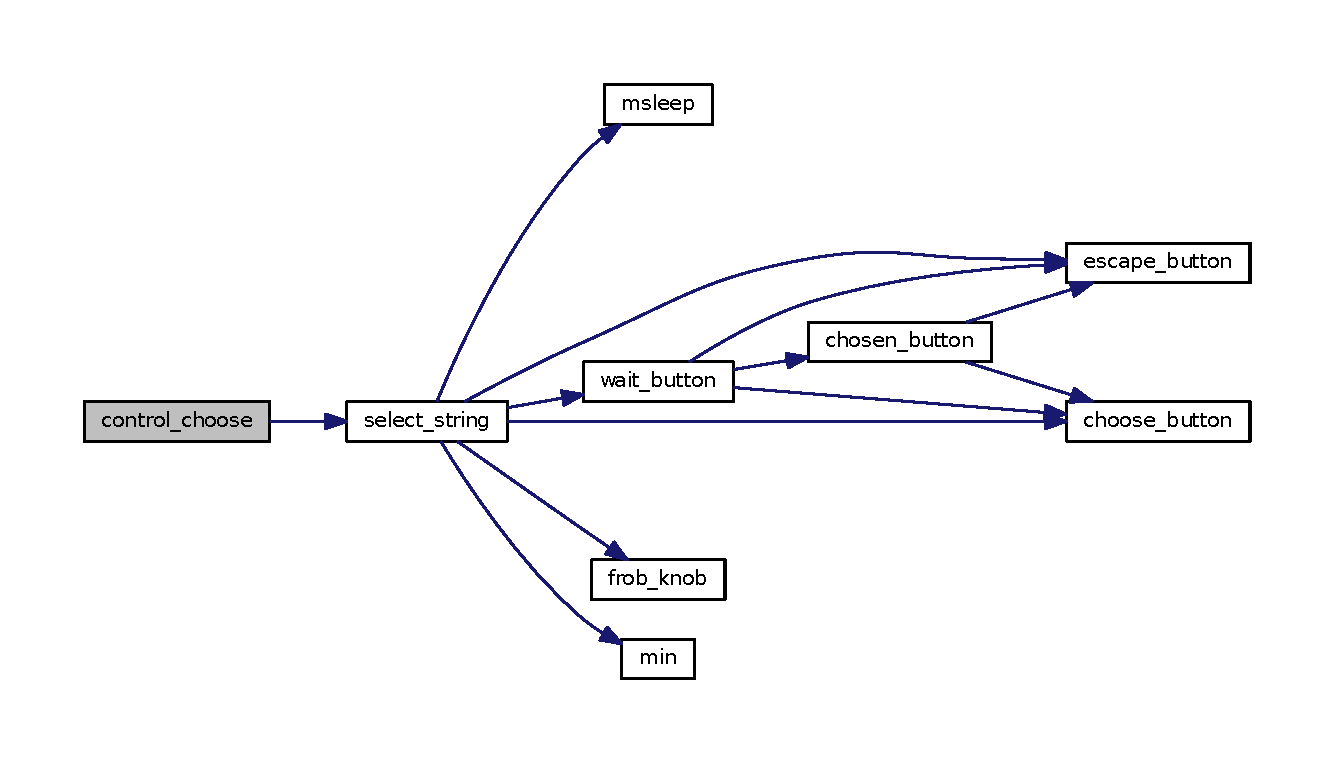
\includegraphics[width=350pt]{diagnostic_8c_aca7443f3516c9e251222934ede56b80b_cgraph}
\end{center}
\end{figure}




Here is the caller graph for this function\-:
\nopagebreak
\begin{figure}[H]
\begin{center}
\leavevmode
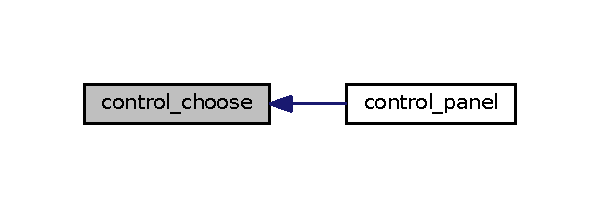
\includegraphics[width=288pt]{diagnostic_8c_aca7443f3516c9e251222934ede56b80b_icgraph}
\end{center}
\end{figure}


\hypertarget{diagnostic_8c_ab93a0ba8748af7794b42a8c381480915}{\index{diagnostic.\-c@{diagnostic.\-c}!control\-\_\-panel@{control\-\_\-panel}}
\index{control\-\_\-panel@{control\-\_\-panel}!diagnostic.c@{diagnostic.\-c}}
\subsubsection[{control\-\_\-panel}]{\setlength{\rightskip}{0pt plus 5cm}void control\-\_\-panel (
\begin{DoxyParamCaption}
{}
\end{DoxyParamCaption}
)}}\label{diagnostic_8c_ab93a0ba8748af7794b42a8c381480915}


Here is the call graph for this function\-:
\nopagebreak
\begin{figure}[H]
\begin{center}
\leavevmode
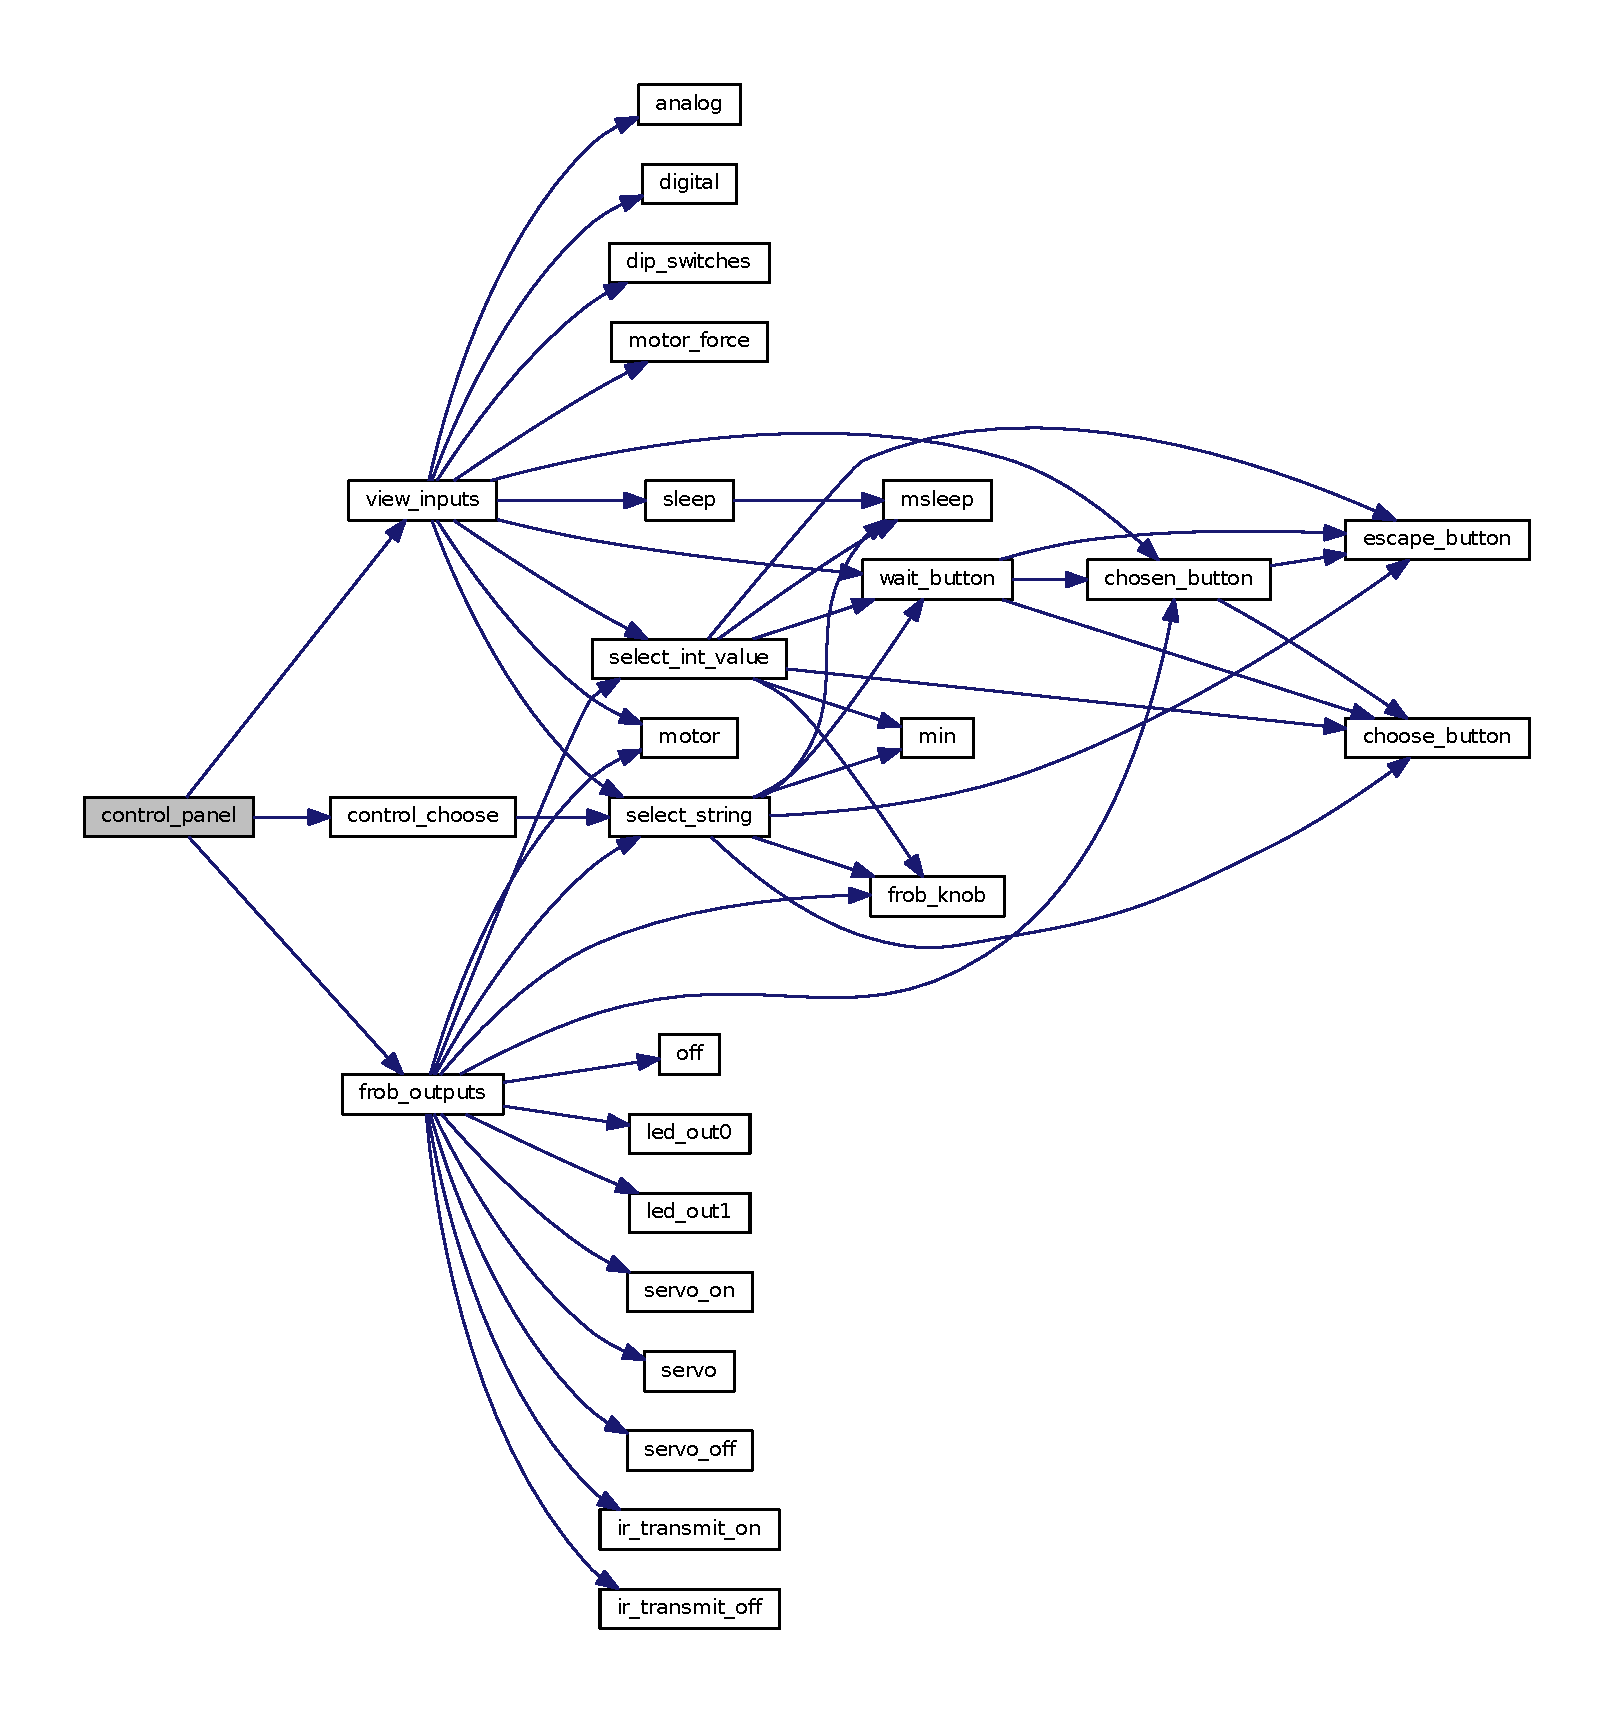
\includegraphics[width=350pt]{diagnostic_8c_ab93a0ba8748af7794b42a8c381480915_cgraph}
\end{center}
\end{figure}


\hypertarget{diagnostic_8c_ab50d07079b04faf6898956b052644966}{\index{diagnostic.\-c@{diagnostic.\-c}!frob\-\_\-outputs@{frob\-\_\-outputs}}
\index{frob\-\_\-outputs@{frob\-\_\-outputs}!diagnostic.c@{diagnostic.\-c}}
\subsubsection[{frob\-\_\-outputs}]{\setlength{\rightskip}{0pt plus 5cm}void frob\-\_\-outputs (
\begin{DoxyParamCaption}
{}
\end{DoxyParamCaption}
)}}\label{diagnostic_8c_ab50d07079b04faf6898956b052644966}


Here is the call graph for this function\-:
\nopagebreak
\begin{figure}[H]
\begin{center}
\leavevmode
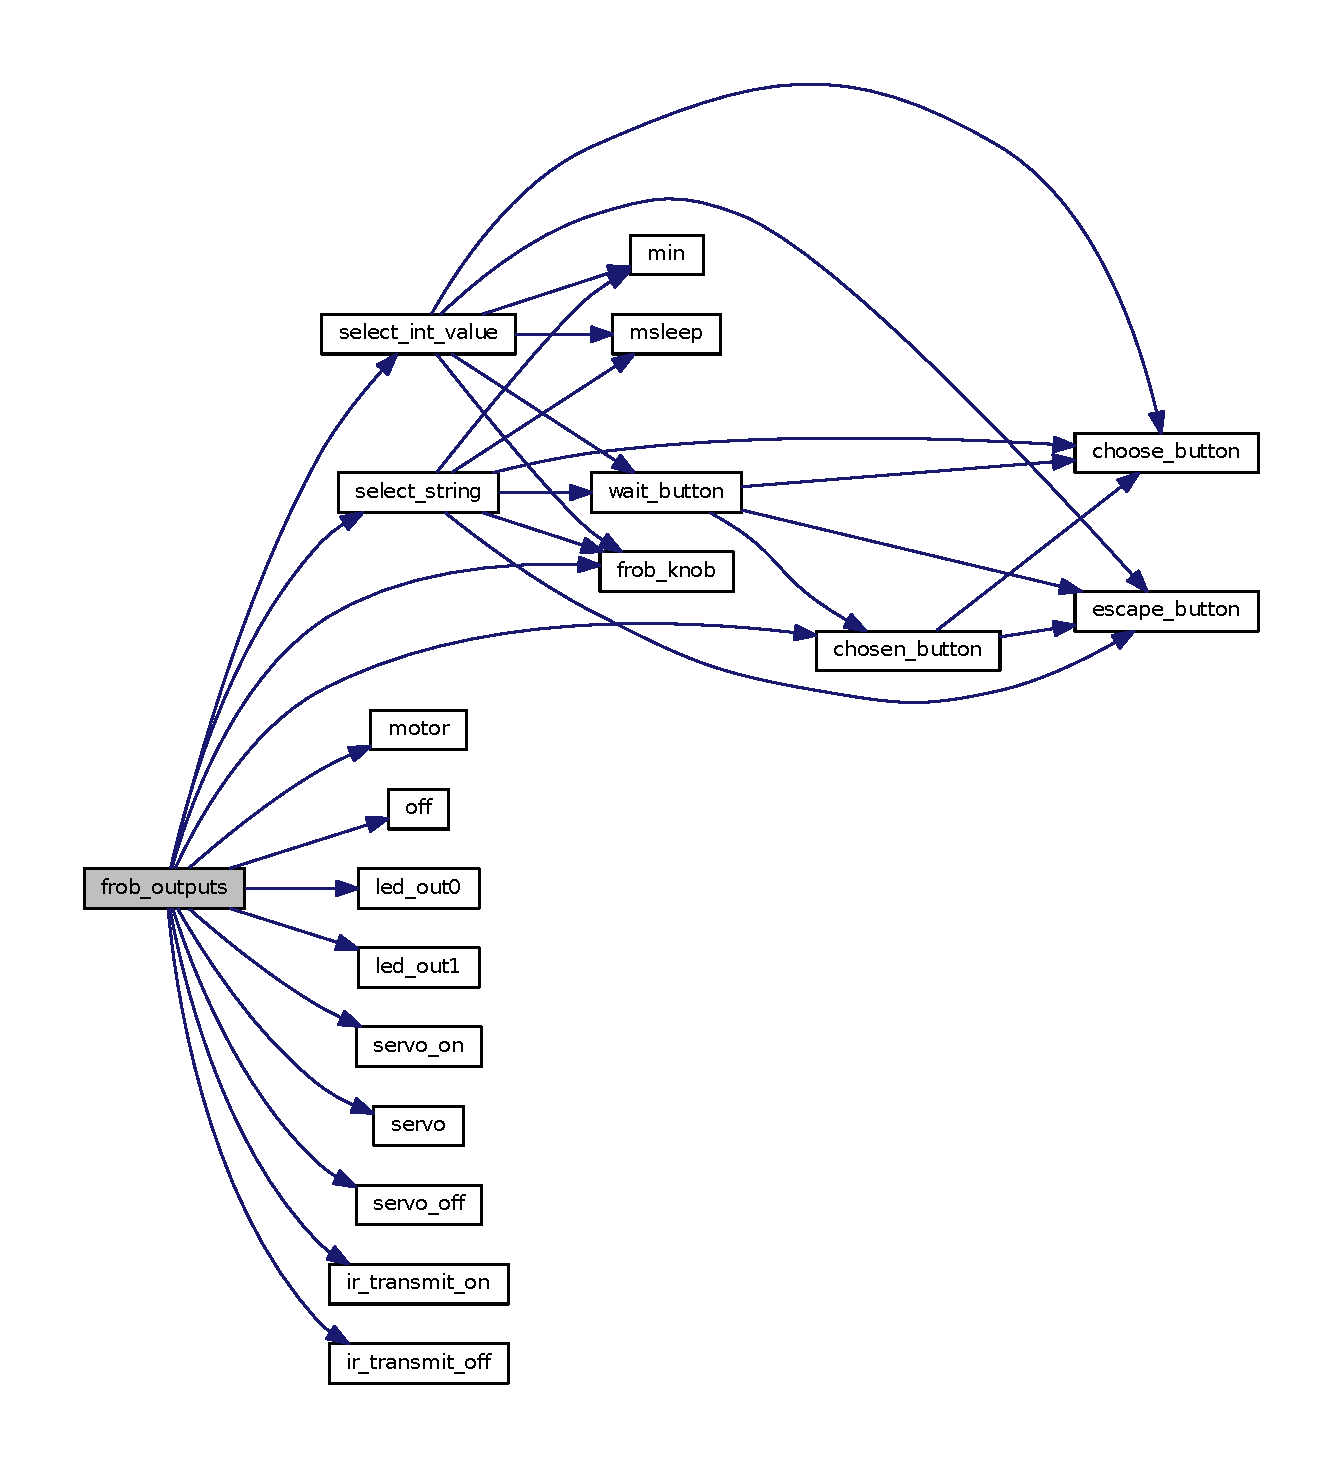
\includegraphics[width=350pt]{diagnostic_8c_ab50d07079b04faf6898956b052644966_cgraph}
\end{center}
\end{figure}




Here is the caller graph for this function\-:
\nopagebreak
\begin{figure}[H]
\begin{center}
\leavevmode
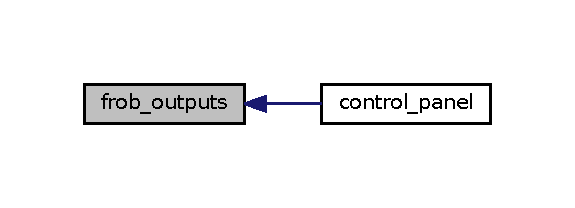
\includegraphics[width=276pt]{diagnostic_8c_ab50d07079b04faf6898956b052644966_icgraph}
\end{center}
\end{figure}


\hypertarget{diagnostic_8c_a42755f36768d92ecf643a73490488309}{\index{diagnostic.\-c@{diagnostic.\-c}!view\-\_\-average\-\_\-port@{view\-\_\-average\-\_\-port}}
\index{view\-\_\-average\-\_\-port@{view\-\_\-average\-\_\-port}!diagnostic.c@{diagnostic.\-c}}
\subsubsection[{view\-\_\-average\-\_\-port}]{\setlength{\rightskip}{0pt plus 5cm}int view\-\_\-average\-\_\-port (
\begin{DoxyParamCaption}
\item[{int}]{port, }
\item[{int}]{samples}
\end{DoxyParamCaption}
)}}\label{diagnostic_8c_a42755f36768d92ecf643a73490488309}


Here is the call graph for this function\-:
\nopagebreak
\begin{figure}[H]
\begin{center}
\leavevmode
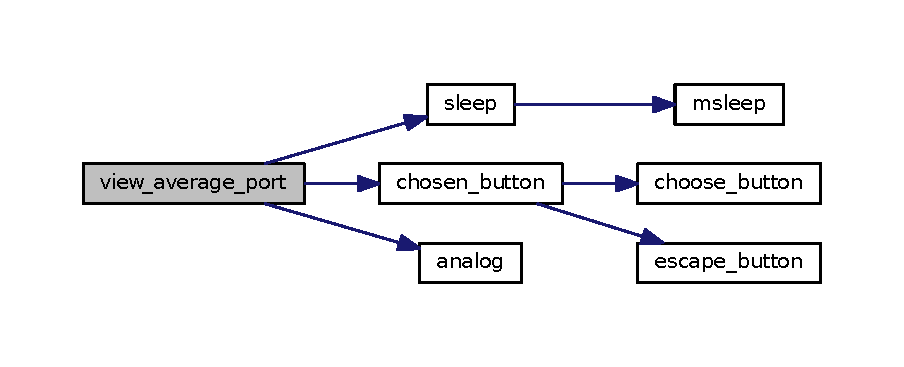
\includegraphics[width=350pt]{diagnostic_8c_a42755f36768d92ecf643a73490488309_cgraph}
\end{center}
\end{figure}


\hypertarget{diagnostic_8c_a9c7615094fa3d462fcd91432cd0d9a3d}{\index{diagnostic.\-c@{diagnostic.\-c}!view\-\_\-inputs@{view\-\_\-inputs}}
\index{view\-\_\-inputs@{view\-\_\-inputs}!diagnostic.c@{diagnostic.\-c}}
\subsubsection[{view\-\_\-inputs}]{\setlength{\rightskip}{0pt plus 5cm}void view\-\_\-inputs (
\begin{DoxyParamCaption}
{}
\end{DoxyParamCaption}
)}}\label{diagnostic_8c_a9c7615094fa3d462fcd91432cd0d9a3d}


Here is the call graph for this function\-:
\nopagebreak
\begin{figure}[H]
\begin{center}
\leavevmode
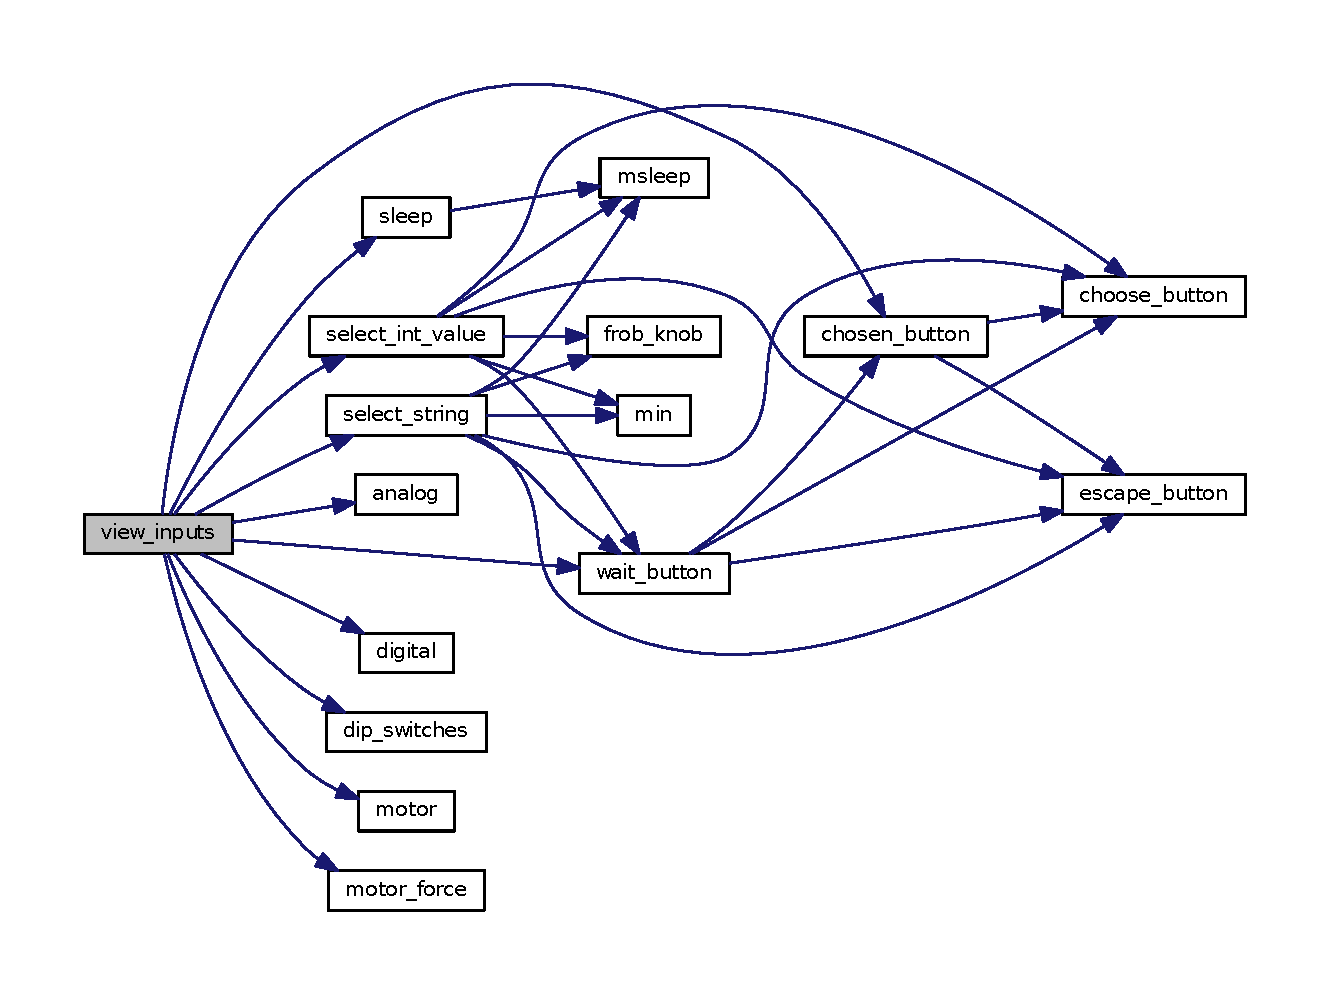
\includegraphics[width=350pt]{diagnostic_8c_a9c7615094fa3d462fcd91432cd0d9a3d_cgraph}
\end{center}
\end{figure}




Here is the caller graph for this function\-:
\nopagebreak
\begin{figure}[H]
\begin{center}
\leavevmode
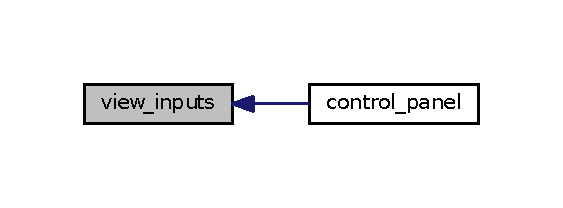
\includegraphics[width=270pt]{diagnostic_8c_a9c7615094fa3d462fcd91432cd0d9a3d_icgraph}
\end{center}
\end{figure}



\hypertarget{encoders_8c}{\section{/root/\-Desktop/ic\-\_\-linux\-\_\-3.1/libs/base/encoders.c File Reference}
\label{encoders_8c}\index{/root/\-Desktop/ic\-\_\-linux\-\_\-3.\-1/libs/base/encoders.\-c@{/root/\-Desktop/ic\-\_\-linux\-\_\-3.\-1/libs/base/encoders.\-c}}
}
\subsection*{Functions}
\begin{DoxyCompactItemize}
\item 
void \hyperlink{encoders_8c_a57729fb729f98b993230bca1c44d5568}{enable\-\_\-encoder} (int i)
\item 
void \hyperlink{encoders_8c_a01bf30d03a129b49dea6be37e236d2ff}{disable\-\_\-encoder} (int i)
\item 
void \hyperlink{encoders_8c_a4de752a5957cb758ec8b59317afda42d}{reset\-\_\-encoder} (int i)
\item 
int \hyperlink{encoders_8c_a68a16dfa47e7e8082342736e4e2672cf}{read\-\_\-encoder} (int i)
\end{DoxyCompactItemize}


\subsection{Function Documentation}
\hypertarget{encoders_8c_a01bf30d03a129b49dea6be37e236d2ff}{\index{encoders.\-c@{encoders.\-c}!disable\-\_\-encoder@{disable\-\_\-encoder}}
\index{disable\-\_\-encoder@{disable\-\_\-encoder}!encoders.c@{encoders.\-c}}
\subsubsection[{disable\-\_\-encoder}]{\setlength{\rightskip}{0pt plus 5cm}void disable\-\_\-encoder (
\begin{DoxyParamCaption}
\item[{int}]{i}
\end{DoxyParamCaption}
)}}\label{encoders_8c_a01bf30d03a129b49dea6be37e236d2ff}
\hypertarget{encoders_8c_a57729fb729f98b993230bca1c44d5568}{\index{encoders.\-c@{encoders.\-c}!enable\-\_\-encoder@{enable\-\_\-encoder}}
\index{enable\-\_\-encoder@{enable\-\_\-encoder}!encoders.c@{encoders.\-c}}
\subsubsection[{enable\-\_\-encoder}]{\setlength{\rightskip}{0pt plus 5cm}void enable\-\_\-encoder (
\begin{DoxyParamCaption}
\item[{int}]{i}
\end{DoxyParamCaption}
)}}\label{encoders_8c_a57729fb729f98b993230bca1c44d5568}
\hypertarget{encoders_8c_a68a16dfa47e7e8082342736e4e2672cf}{\index{encoders.\-c@{encoders.\-c}!read\-\_\-encoder@{read\-\_\-encoder}}
\index{read\-\_\-encoder@{read\-\_\-encoder}!encoders.c@{encoders.\-c}}
\subsubsection[{read\-\_\-encoder}]{\setlength{\rightskip}{0pt plus 5cm}int read\-\_\-encoder (
\begin{DoxyParamCaption}
\item[{int}]{i}
\end{DoxyParamCaption}
)}}\label{encoders_8c_a68a16dfa47e7e8082342736e4e2672cf}
\hypertarget{encoders_8c_a4de752a5957cb758ec8b59317afda42d}{\index{encoders.\-c@{encoders.\-c}!reset\-\_\-encoder@{reset\-\_\-encoder}}
\index{reset\-\_\-encoder@{reset\-\_\-encoder}!encoders.c@{encoders.\-c}}
\subsubsection[{reset\-\_\-encoder}]{\setlength{\rightskip}{0pt plus 5cm}void reset\-\_\-encoder (
\begin{DoxyParamCaption}
\item[{int}]{i}
\end{DoxyParamCaption}
)}}\label{encoders_8c_a4de752a5957cb758ec8b59317afda42d}

\hypertarget{base_2lib__ic_8c}{\section{/root/\-Desktop/rug-\/warrior/libs/base/lib\-\_\-ic.c File Reference}
\label{base_2lib__ic_8c}\index{/root/\-Desktop/rug-\/warrior/libs/base/lib\-\_\-ic.\-c@{/root/\-Desktop/rug-\/warrior/libs/base/lib\-\_\-ic.\-c}}
}
\subsection*{Functions}
\begin{DoxyCompactItemize}
\item 
void \hyperlink{base_2lib__ic_8c_a6089a104ffb48b4c9705527f5287c418}{reset\-\_\-system\-\_\-time} ()
\item 
float \hyperlink{base_2lib__ic_8c_ab53334924c8ee90693b8d48d8f74793d}{seconds} ()
\item 
void \hyperlink{base_2lib__ic_8c_aa5113ec47ecf6d5c15614c9353cb9a08}{sleep} (float \hyperlink{lib__rw11_8c_ab53334924c8ee90693b8d48d8f74793d}{seconds})
\item 
void \hyperlink{base_2lib__ic_8c_aa3650dfb953be0fa6fb4e6a625d3f777}{msleep} (long msec)
\item 
void \hyperlink{base_2lib__ic_8c_a912dfbf994f4d4c7dff5aa2540ae4400}{beep} ()
\item 
void \hyperlink{base_2lib__ic_8c_aabe762cad0063d9271131f3cc306a0e8}{tone} (float frequency, float length)
\item 
void \hyperlink{base_2lib__ic_8c_ac01536f2a7ceb0d4c7e5e6a6d59c3871}{beeper\-\_\-on} ()
\item 
void \hyperlink{base_2lib__ic_8c_a35b95a4506fe38aa8c942b178cdda428}{beeper\-\_\-off} ()
\item 
void \hyperlink{base_2lib__ic_8c_aebfeaced338ec2353b5d133eebfb3ebb}{set\-\_\-beeper\-\_\-pitch} (float frequency)
\item 
long \hyperlink{base_2lib__ic_8c_a3ced1c4d929dec5fc84c7a905001a948}{timer\-\_\-create\-\_\-mseconds} (long timeout)
\item 
long \hyperlink{base_2lib__ic_8c_a103a241f9babfefa4a5a754bb2368253}{timer\-\_\-create\-\_\-seconds} (float timeout)
\item 
int \hyperlink{base_2lib__ic_8c_a2a0f0ec3bd9ebf537a7a728b9b837f0e}{timer\-\_\-done} (long timer)
\item 
int \hyperlink{base_2lib__ic_8c_afa28db0c35c02b77341a6bed7aac0cb4}{analog} (int port)
\item 
void \hyperlink{base_2lib__ic_8c_a1299acec6790d8d455483b14b1917c37}{hog\-\_\-processor} ()
\end{DoxyCompactItemize}
\subsection*{Variables}
\begin{DoxyCompactItemize}
\item 
persistent int \hyperlink{base_2lib__ic_8c_a1655ba35f7c4737369c27c3c5f49b6d0}{test\-\_\-number}
\end{DoxyCompactItemize}


\subsection{Function Documentation}
\hypertarget{base_2lib__ic_8c_afa28db0c35c02b77341a6bed7aac0cb4}{\index{base/lib\-\_\-ic.\-c@{base/lib\-\_\-ic.\-c}!analog@{analog}}
\index{analog@{analog}!base/lib_ic.c@{base/lib\-\_\-ic.\-c}}
\subsubsection[{analog}]{\setlength{\rightskip}{0pt plus 5cm}int analog (
\begin{DoxyParamCaption}
\item[{int}]{port}
\end{DoxyParamCaption}
)}}\label{base_2lib__ic_8c_afa28db0c35c02b77341a6bed7aac0cb4}


Here is the caller graph for this function\-:
\nopagebreak
\begin{figure}[H]
\begin{center}
\leavevmode
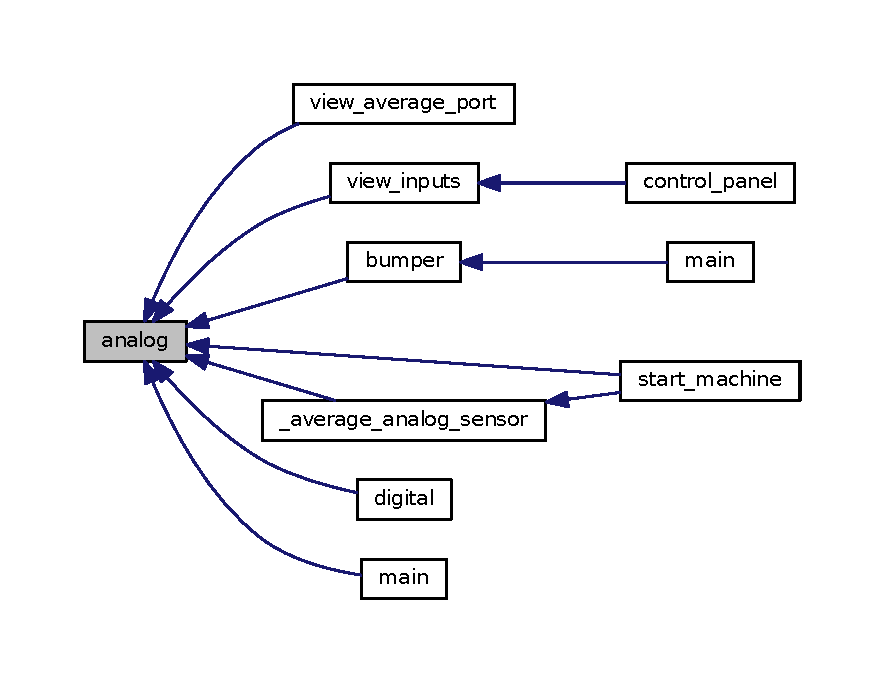
\includegraphics[width=350pt]{base_2lib__ic_8c_afa28db0c35c02b77341a6bed7aac0cb4_icgraph}
\end{center}
\end{figure}


\hypertarget{base_2lib__ic_8c_a912dfbf994f4d4c7dff5aa2540ae4400}{\index{base/lib\-\_\-ic.\-c@{base/lib\-\_\-ic.\-c}!beep@{beep}}
\index{beep@{beep}!base/lib_ic.c@{base/lib\-\_\-ic.\-c}}
\subsubsection[{beep}]{\setlength{\rightskip}{0pt plus 5cm}void beep (
\begin{DoxyParamCaption}
{}
\end{DoxyParamCaption}
)}}\label{base_2lib__ic_8c_a912dfbf994f4d4c7dff5aa2540ae4400}


Here is the call graph for this function\-:
\nopagebreak
\begin{figure}[H]
\begin{center}
\leavevmode
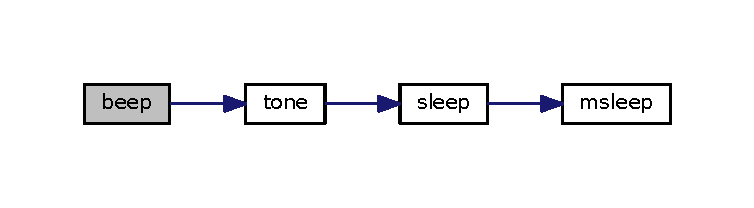
\includegraphics[width=350pt]{base_2lib__ic_8c_a912dfbf994f4d4c7dff5aa2540ae4400_cgraph}
\end{center}
\end{figure}




Here is the caller graph for this function\-:
\nopagebreak
\begin{figure}[H]
\begin{center}
\leavevmode
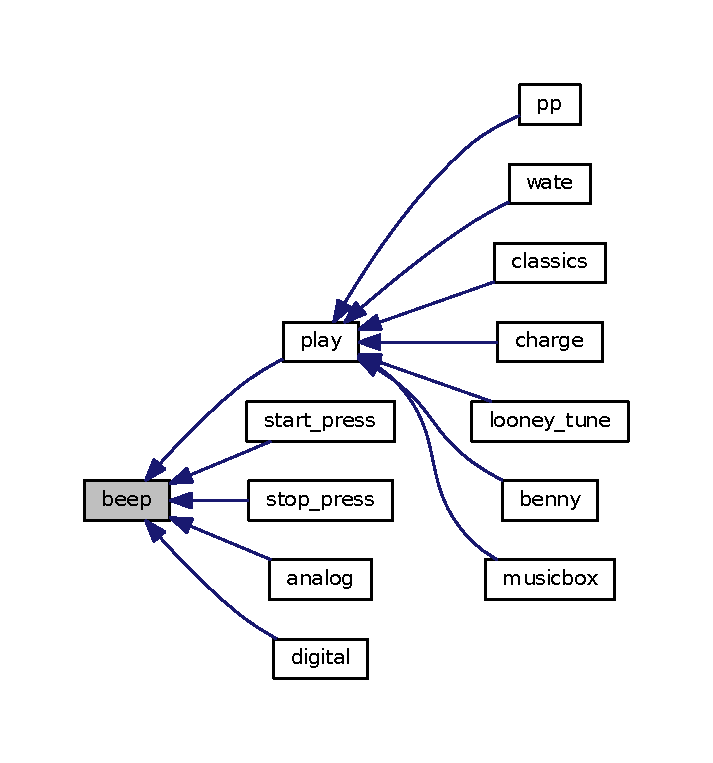
\includegraphics[width=342pt]{base_2lib__ic_8c_a912dfbf994f4d4c7dff5aa2540ae4400_icgraph}
\end{center}
\end{figure}


\hypertarget{base_2lib__ic_8c_a35b95a4506fe38aa8c942b178cdda428}{\index{base/lib\-\_\-ic.\-c@{base/lib\-\_\-ic.\-c}!beeper\-\_\-off@{beeper\-\_\-off}}
\index{beeper\-\_\-off@{beeper\-\_\-off}!base/lib_ic.c@{base/lib\-\_\-ic.\-c}}
\subsubsection[{beeper\-\_\-off}]{\setlength{\rightskip}{0pt plus 5cm}void beeper\-\_\-off (
\begin{DoxyParamCaption}
{}
\end{DoxyParamCaption}
)}}\label{base_2lib__ic_8c_a35b95a4506fe38aa8c942b178cdda428}


Here is the caller graph for this function\-:
\nopagebreak
\begin{figure}[H]
\begin{center}
\leavevmode
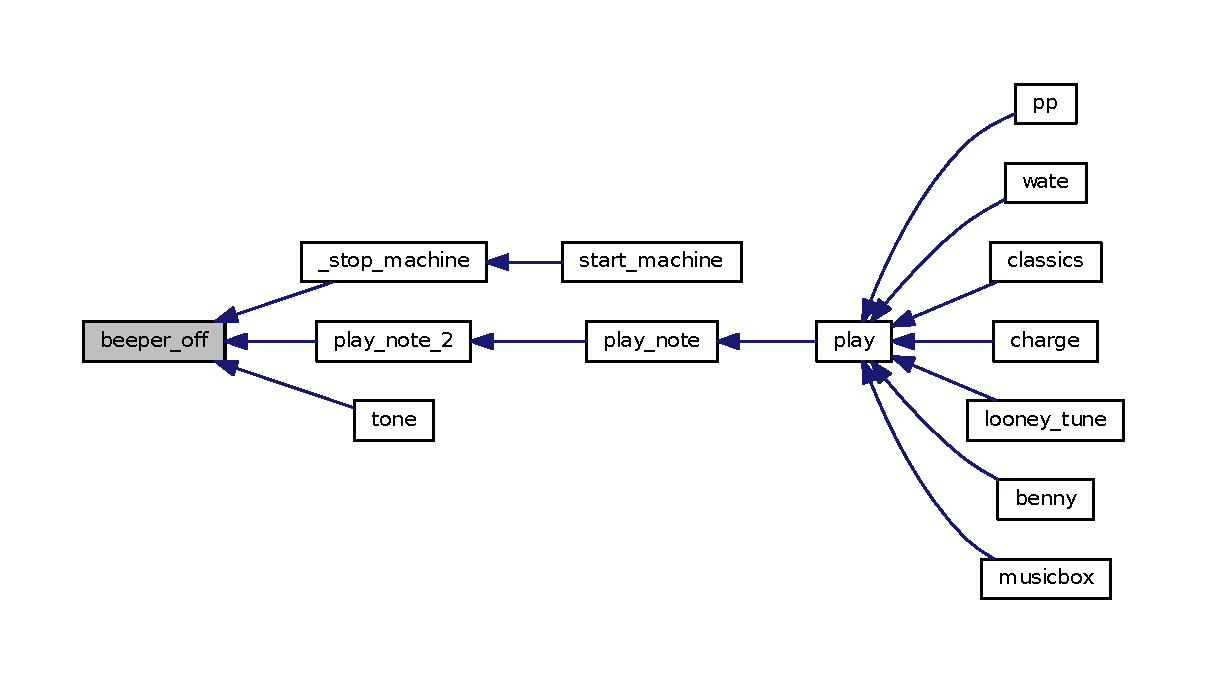
\includegraphics[width=350pt]{base_2lib__ic_8c_a35b95a4506fe38aa8c942b178cdda428_icgraph}
\end{center}
\end{figure}


\hypertarget{base_2lib__ic_8c_ac01536f2a7ceb0d4c7e5e6a6d59c3871}{\index{base/lib\-\_\-ic.\-c@{base/lib\-\_\-ic.\-c}!beeper\-\_\-on@{beeper\-\_\-on}}
\index{beeper\-\_\-on@{beeper\-\_\-on}!base/lib_ic.c@{base/lib\-\_\-ic.\-c}}
\subsubsection[{beeper\-\_\-on}]{\setlength{\rightskip}{0pt plus 5cm}void beeper\-\_\-on (
\begin{DoxyParamCaption}
{}
\end{DoxyParamCaption}
)}}\label{base_2lib__ic_8c_ac01536f2a7ceb0d4c7e5e6a6d59c3871}


Here is the caller graph for this function\-:
\nopagebreak
\begin{figure}[H]
\begin{center}
\leavevmode
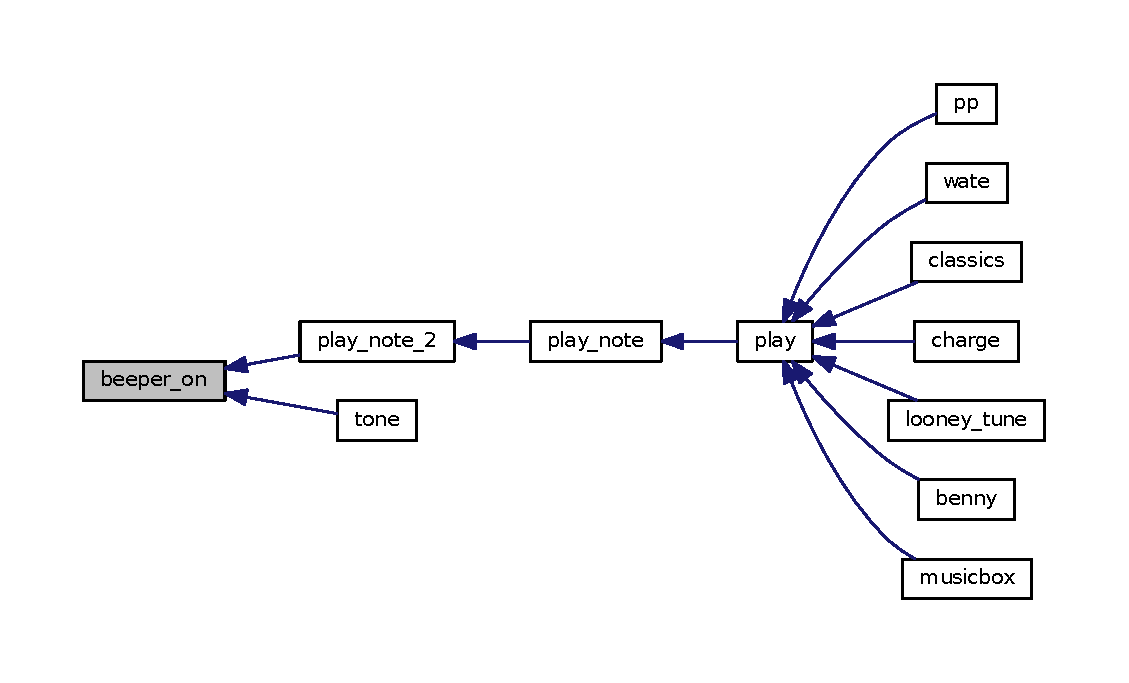
\includegraphics[width=350pt]{base_2lib__ic_8c_ac01536f2a7ceb0d4c7e5e6a6d59c3871_icgraph}
\end{center}
\end{figure}


\hypertarget{base_2lib__ic_8c_a1299acec6790d8d455483b14b1917c37}{\index{base/lib\-\_\-ic.\-c@{base/lib\-\_\-ic.\-c}!hog\-\_\-processor@{hog\-\_\-processor}}
\index{hog\-\_\-processor@{hog\-\_\-processor}!base/lib_ic.c@{base/lib\-\_\-ic.\-c}}
\subsubsection[{hog\-\_\-processor}]{\setlength{\rightskip}{0pt plus 5cm}void hog\-\_\-processor (
\begin{DoxyParamCaption}
{}
\end{DoxyParamCaption}
)}}\label{base_2lib__ic_8c_a1299acec6790d8d455483b14b1917c37}


Here is the caller graph for this function\-:
\nopagebreak
\begin{figure}[H]
\begin{center}
\leavevmode
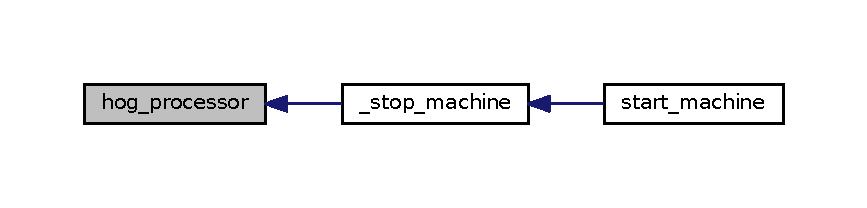
\includegraphics[width=350pt]{base_2lib__ic_8c_a1299acec6790d8d455483b14b1917c37_icgraph}
\end{center}
\end{figure}


\hypertarget{base_2lib__ic_8c_aa3650dfb953be0fa6fb4e6a625d3f777}{\index{base/lib\-\_\-ic.\-c@{base/lib\-\_\-ic.\-c}!msleep@{msleep}}
\index{msleep@{msleep}!base/lib_ic.c@{base/lib\-\_\-ic.\-c}}
\subsubsection[{msleep}]{\setlength{\rightskip}{0pt plus 5cm}void msleep (
\begin{DoxyParamCaption}
\item[{long}]{msec}
\end{DoxyParamCaption}
)}}\label{base_2lib__ic_8c_aa3650dfb953be0fa6fb4e6a625d3f777}


Here is the caller graph for this function\-:
\nopagebreak
\begin{figure}[H]
\begin{center}
\leavevmode
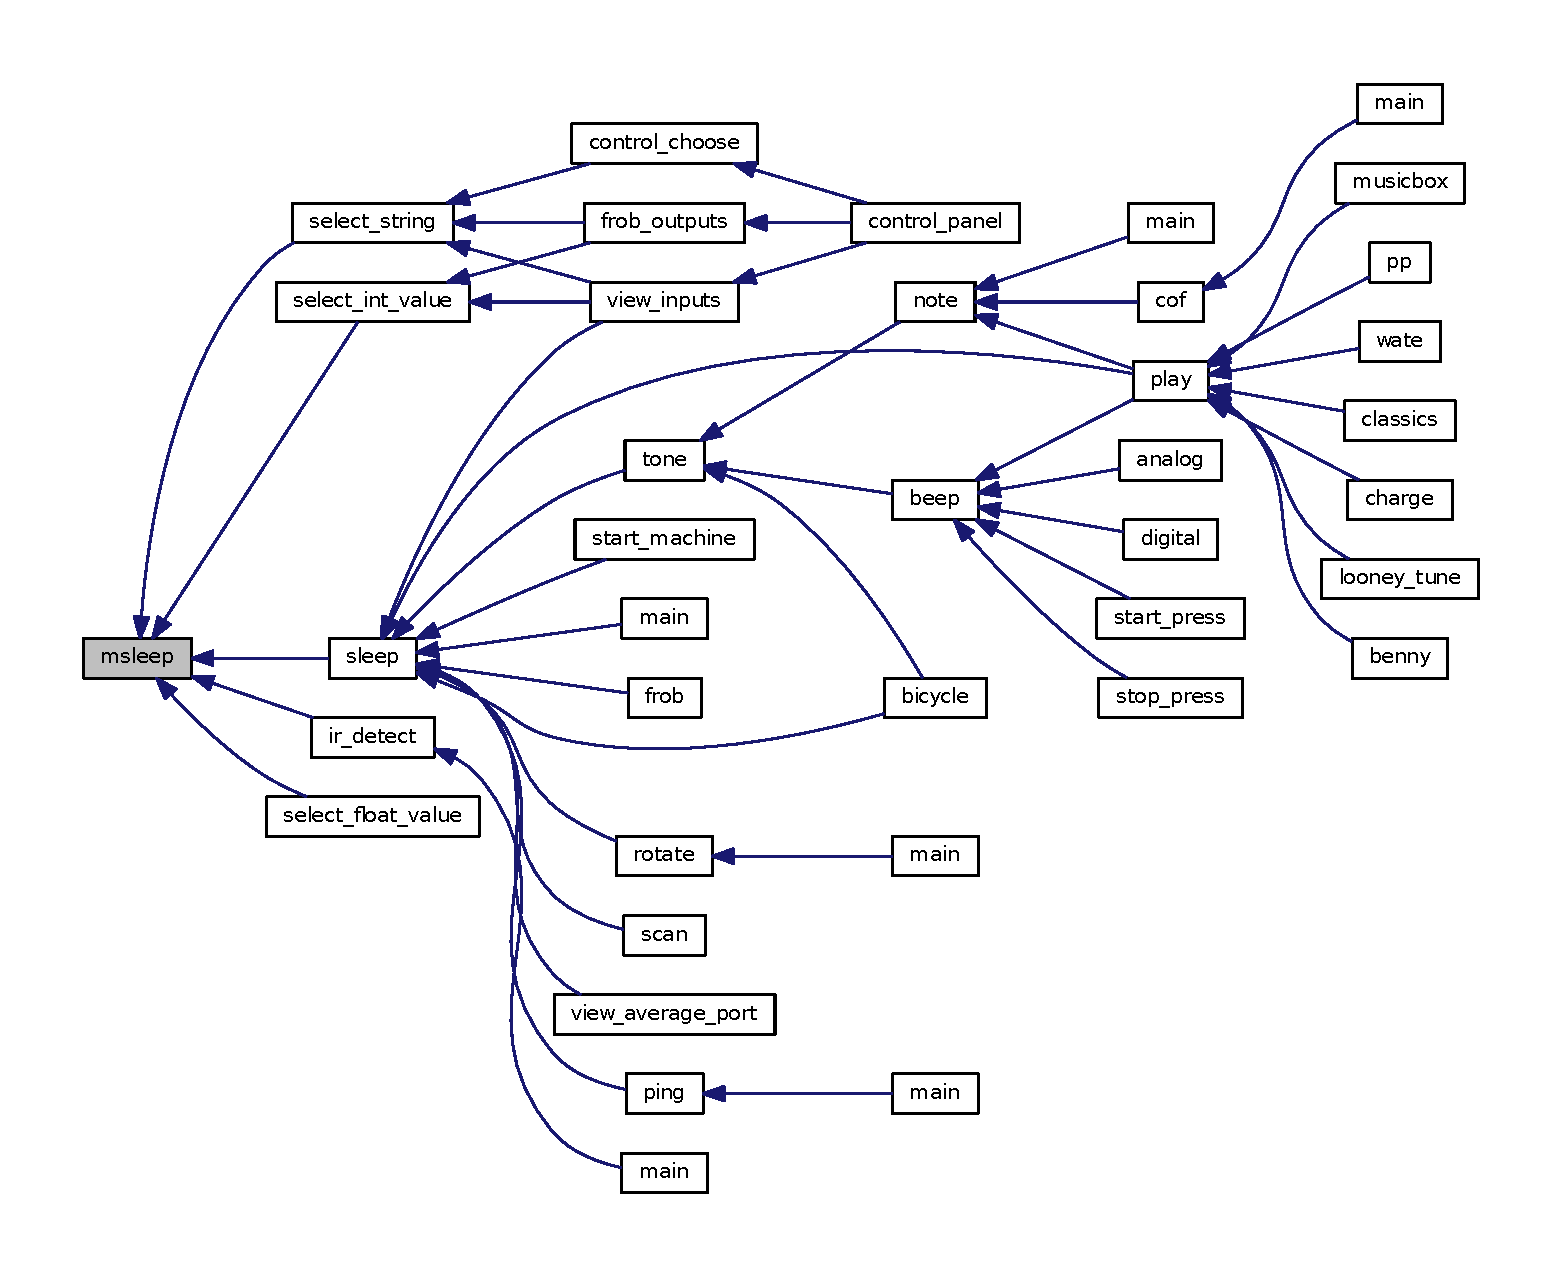
\includegraphics[width=350pt]{base_2lib__ic_8c_aa3650dfb953be0fa6fb4e6a625d3f777_icgraph}
\end{center}
\end{figure}


\hypertarget{base_2lib__ic_8c_a6089a104ffb48b4c9705527f5287c418}{\index{base/lib\-\_\-ic.\-c@{base/lib\-\_\-ic.\-c}!reset\-\_\-system\-\_\-time@{reset\-\_\-system\-\_\-time}}
\index{reset\-\_\-system\-\_\-time@{reset\-\_\-system\-\_\-time}!base/lib_ic.c@{base/lib\-\_\-ic.\-c}}
\subsubsection[{reset\-\_\-system\-\_\-time}]{\setlength{\rightskip}{0pt plus 5cm}void reset\-\_\-system\-\_\-time (
\begin{DoxyParamCaption}
{}
\end{DoxyParamCaption}
)}}\label{base_2lib__ic_8c_a6089a104ffb48b4c9705527f5287c418}


Here is the caller graph for this function\-:
\nopagebreak
\begin{figure}[H]
\begin{center}
\leavevmode
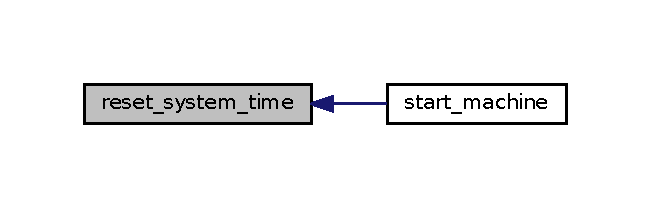
\includegraphics[width=312pt]{base_2lib__ic_8c_a6089a104ffb48b4c9705527f5287c418_icgraph}
\end{center}
\end{figure}


\hypertarget{base_2lib__ic_8c_ab53334924c8ee90693b8d48d8f74793d}{\index{base/lib\-\_\-ic.\-c@{base/lib\-\_\-ic.\-c}!seconds@{seconds}}
\index{seconds@{seconds}!base/lib_ic.c@{base/lib\-\_\-ic.\-c}}
\subsubsection[{seconds}]{\setlength{\rightskip}{0pt plus 5cm}float seconds (
\begin{DoxyParamCaption}
{}
\end{DoxyParamCaption}
)}}\label{base_2lib__ic_8c_ab53334924c8ee90693b8d48d8f74793d}


Here is the caller graph for this function\-:
\nopagebreak
\begin{figure}[H]
\begin{center}
\leavevmode
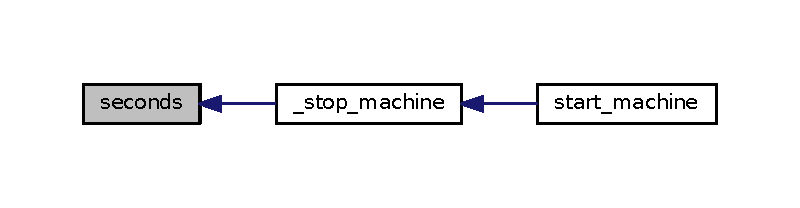
\includegraphics[width=350pt]{base_2lib__ic_8c_ab53334924c8ee90693b8d48d8f74793d_icgraph}
\end{center}
\end{figure}


\hypertarget{base_2lib__ic_8c_aebfeaced338ec2353b5d133eebfb3ebb}{\index{base/lib\-\_\-ic.\-c@{base/lib\-\_\-ic.\-c}!set\-\_\-beeper\-\_\-pitch@{set\-\_\-beeper\-\_\-pitch}}
\index{set\-\_\-beeper\-\_\-pitch@{set\-\_\-beeper\-\_\-pitch}!base/lib_ic.c@{base/lib\-\_\-ic.\-c}}
\subsubsection[{set\-\_\-beeper\-\_\-pitch}]{\setlength{\rightskip}{0pt plus 5cm}void set\-\_\-beeper\-\_\-pitch (
\begin{DoxyParamCaption}
\item[{float}]{frequency}
\end{DoxyParamCaption}
)}}\label{base_2lib__ic_8c_aebfeaced338ec2353b5d133eebfb3ebb}


Here is the caller graph for this function\-:
\nopagebreak
\begin{figure}[H]
\begin{center}
\leavevmode
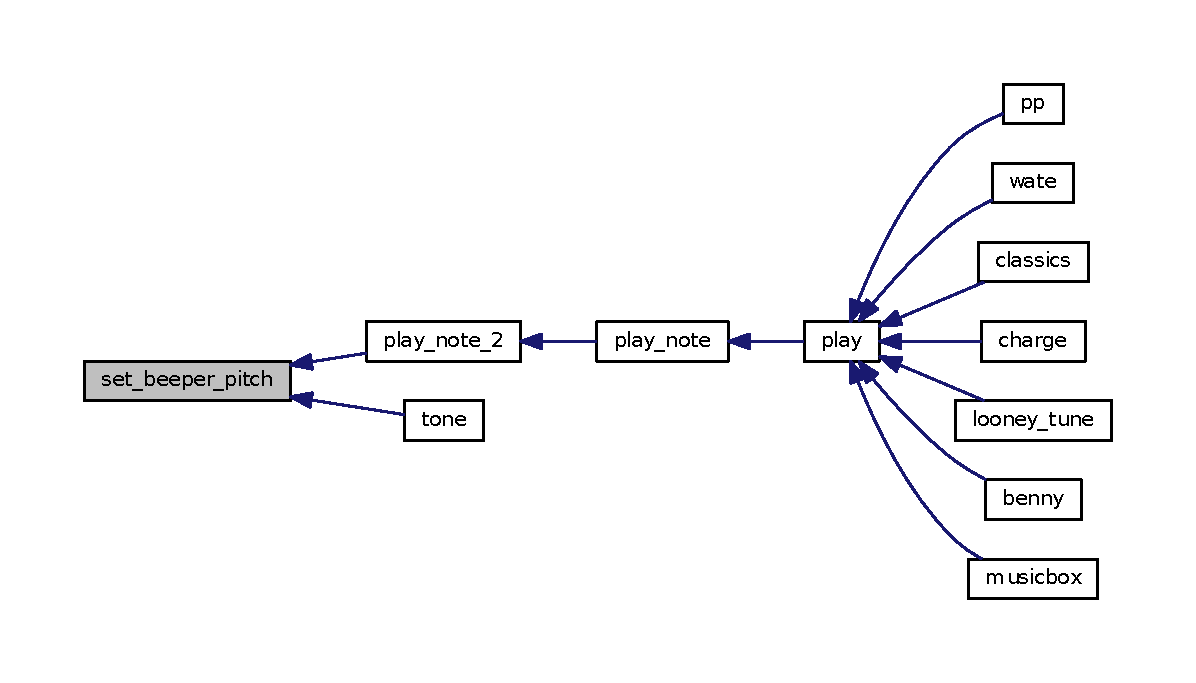
\includegraphics[width=350pt]{base_2lib__ic_8c_aebfeaced338ec2353b5d133eebfb3ebb_icgraph}
\end{center}
\end{figure}


\hypertarget{base_2lib__ic_8c_aa5113ec47ecf6d5c15614c9353cb9a08}{\index{base/lib\-\_\-ic.\-c@{base/lib\-\_\-ic.\-c}!sleep@{sleep}}
\index{sleep@{sleep}!base/lib_ic.c@{base/lib\-\_\-ic.\-c}}
\subsubsection[{sleep}]{\setlength{\rightskip}{0pt plus 5cm}void sleep (
\begin{DoxyParamCaption}
\item[{float}]{seconds}
\end{DoxyParamCaption}
)}}\label{base_2lib__ic_8c_aa5113ec47ecf6d5c15614c9353cb9a08}


Here is the call graph for this function\-:
\nopagebreak
\begin{figure}[H]
\begin{center}
\leavevmode
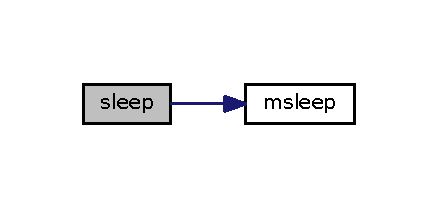
\includegraphics[width=210pt]{base_2lib__ic_8c_aa5113ec47ecf6d5c15614c9353cb9a08_cgraph}
\end{center}
\end{figure}




Here is the caller graph for this function\-:
\nopagebreak
\begin{figure}[H]
\begin{center}
\leavevmode
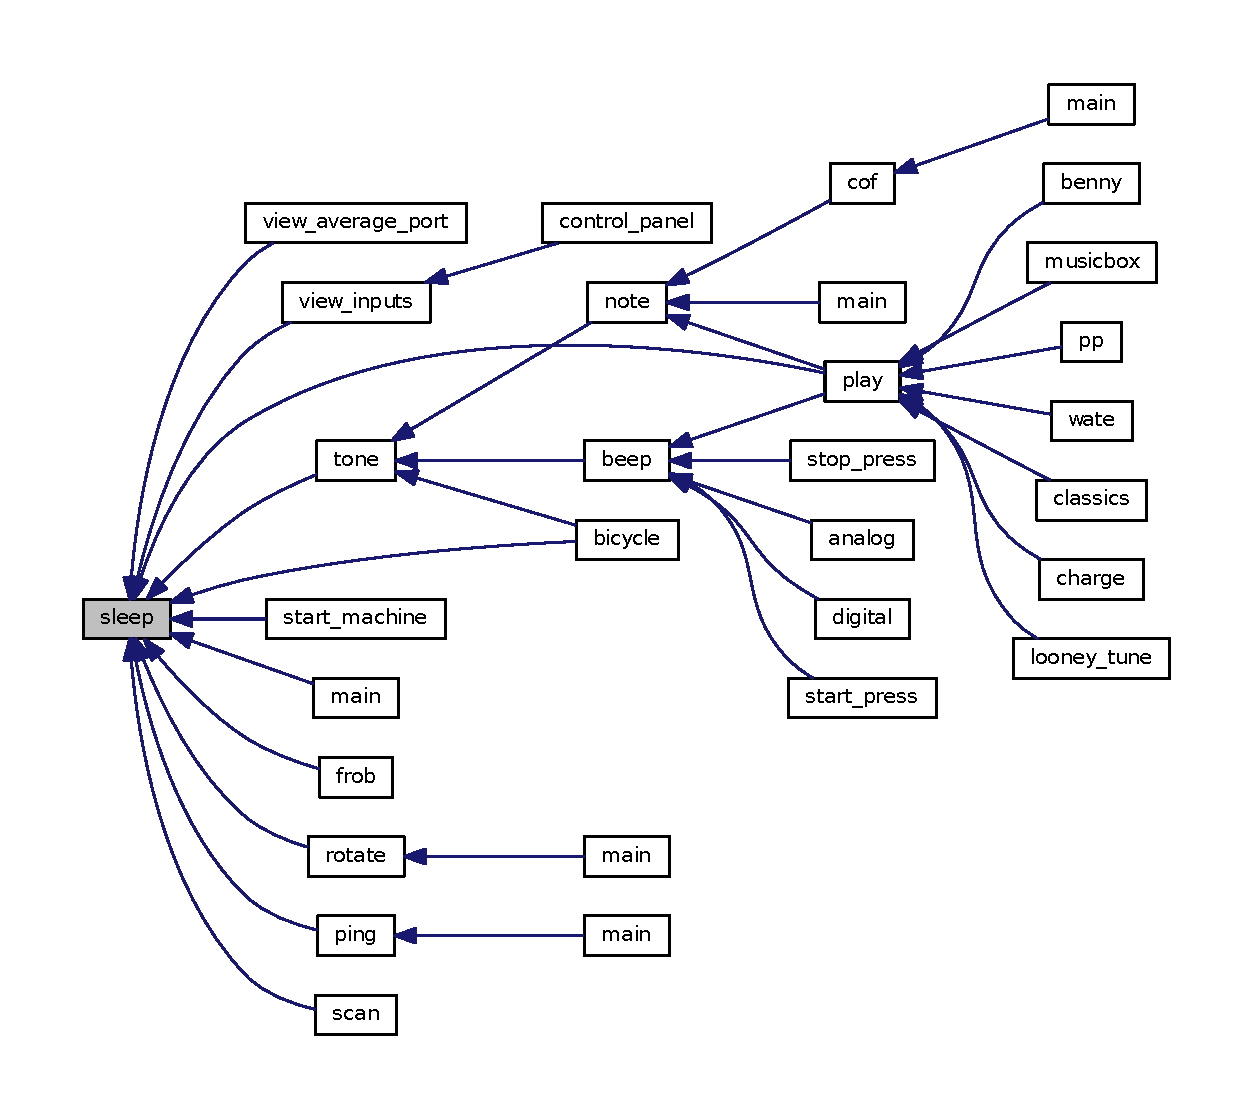
\includegraphics[width=350pt]{base_2lib__ic_8c_aa5113ec47ecf6d5c15614c9353cb9a08_icgraph}
\end{center}
\end{figure}


\hypertarget{base_2lib__ic_8c_a3ced1c4d929dec5fc84c7a905001a948}{\index{base/lib\-\_\-ic.\-c@{base/lib\-\_\-ic.\-c}!timer\-\_\-create\-\_\-mseconds@{timer\-\_\-create\-\_\-mseconds}}
\index{timer\-\_\-create\-\_\-mseconds@{timer\-\_\-create\-\_\-mseconds}!base/lib_ic.c@{base/lib\-\_\-ic.\-c}}
\subsubsection[{timer\-\_\-create\-\_\-mseconds}]{\setlength{\rightskip}{0pt plus 5cm}long timer\-\_\-create\-\_\-mseconds (
\begin{DoxyParamCaption}
\item[{long}]{timeout}
\end{DoxyParamCaption}
)}}\label{base_2lib__ic_8c_a3ced1c4d929dec5fc84c7a905001a948}
\hypertarget{base_2lib__ic_8c_a103a241f9babfefa4a5a754bb2368253}{\index{base/lib\-\_\-ic.\-c@{base/lib\-\_\-ic.\-c}!timer\-\_\-create\-\_\-seconds@{timer\-\_\-create\-\_\-seconds}}
\index{timer\-\_\-create\-\_\-seconds@{timer\-\_\-create\-\_\-seconds}!base/lib_ic.c@{base/lib\-\_\-ic.\-c}}
\subsubsection[{timer\-\_\-create\-\_\-seconds}]{\setlength{\rightskip}{0pt plus 5cm}long timer\-\_\-create\-\_\-seconds (
\begin{DoxyParamCaption}
\item[{float}]{timeout}
\end{DoxyParamCaption}
)}}\label{base_2lib__ic_8c_a103a241f9babfefa4a5a754bb2368253}
\hypertarget{base_2lib__ic_8c_a2a0f0ec3bd9ebf537a7a728b9b837f0e}{\index{base/lib\-\_\-ic.\-c@{base/lib\-\_\-ic.\-c}!timer\-\_\-done@{timer\-\_\-done}}
\index{timer\-\_\-done@{timer\-\_\-done}!base/lib_ic.c@{base/lib\-\_\-ic.\-c}}
\subsubsection[{timer\-\_\-done}]{\setlength{\rightskip}{0pt plus 5cm}int timer\-\_\-done (
\begin{DoxyParamCaption}
\item[{long}]{timer}
\end{DoxyParamCaption}
)}}\label{base_2lib__ic_8c_a2a0f0ec3bd9ebf537a7a728b9b837f0e}
\hypertarget{base_2lib__ic_8c_aabe762cad0063d9271131f3cc306a0e8}{\index{base/lib\-\_\-ic.\-c@{base/lib\-\_\-ic.\-c}!tone@{tone}}
\index{tone@{tone}!base/lib_ic.c@{base/lib\-\_\-ic.\-c}}
\subsubsection[{tone}]{\setlength{\rightskip}{0pt plus 5cm}void tone (
\begin{DoxyParamCaption}
\item[{float}]{frequency, }
\item[{float}]{length}
\end{DoxyParamCaption}
)}}\label{base_2lib__ic_8c_aabe762cad0063d9271131f3cc306a0e8}


Here is the call graph for this function\-:
\nopagebreak
\begin{figure}[H]
\begin{center}
\leavevmode
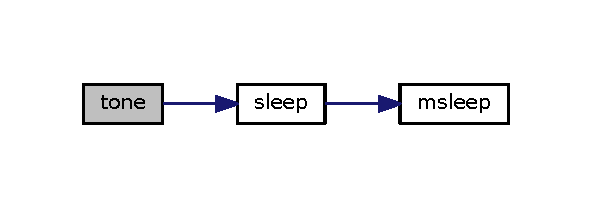
\includegraphics[width=284pt]{base_2lib__ic_8c_aabe762cad0063d9271131f3cc306a0e8_cgraph}
\end{center}
\end{figure}




Here is the caller graph for this function\-:
\nopagebreak
\begin{figure}[H]
\begin{center}
\leavevmode
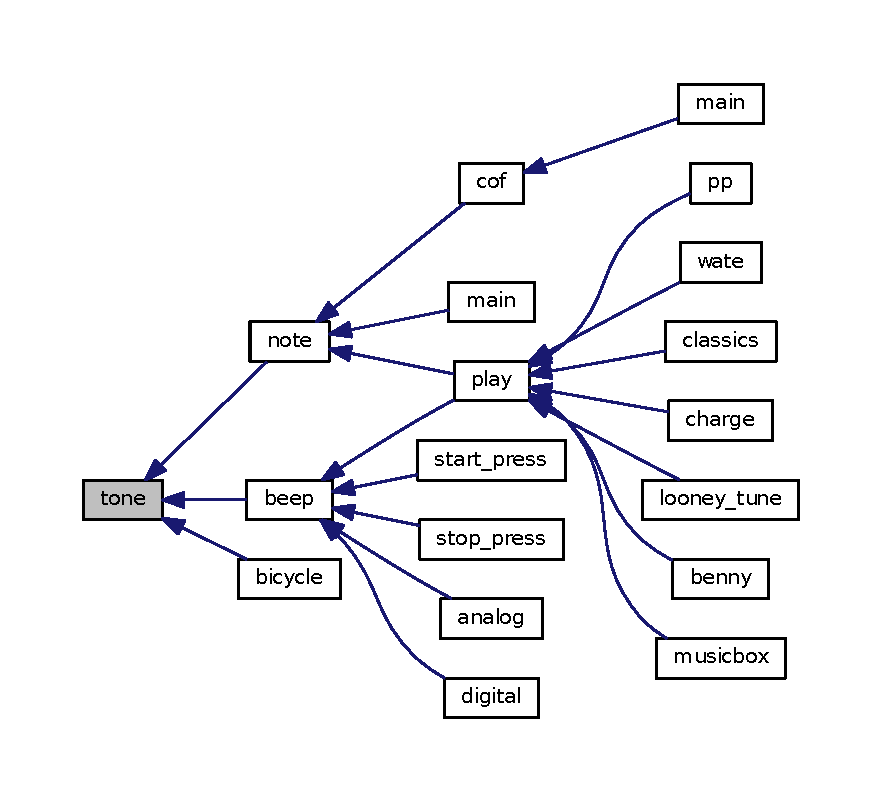
\includegraphics[width=350pt]{base_2lib__ic_8c_aabe762cad0063d9271131f3cc306a0e8_icgraph}
\end{center}
\end{figure}




\subsection{Variable Documentation}
\hypertarget{base_2lib__ic_8c_a1655ba35f7c4737369c27c3c5f49b6d0}{\index{base/lib\-\_\-ic.\-c@{base/lib\-\_\-ic.\-c}!test\-\_\-number@{test\-\_\-number}}
\index{test\-\_\-number@{test\-\_\-number}!base/lib_ic.c@{base/lib\-\_\-ic.\-c}}
\subsubsection[{test\-\_\-number}]{\setlength{\rightskip}{0pt plus 5cm}persistent int test\-\_\-number}}\label{base_2lib__ic_8c_a1655ba35f7c4737369c27c3c5f49b6d0}

\hypertarget{firmware_2lib__ic_8c}{\section{/root/\-Desktop/ic\-\_\-linux\-\_\-3.1/libs/firmware/lib\-\_\-ic.c File Reference}
\label{firmware_2lib__ic_8c}\index{/root/\-Desktop/ic\-\_\-linux\-\_\-3.\-1/libs/firmware/lib\-\_\-ic.\-c@{/root/\-Desktop/ic\-\_\-linux\-\_\-3.\-1/libs/firmware/lib\-\_\-ic.\-c}}
}
\subsection*{Functions}
\begin{DoxyCompactItemize}
\item 
void \hyperlink{firmware_2lib__ic_8c_a6089a104ffb48b4c9705527f5287c418}{reset\-\_\-system\-\_\-time} ()
\item 
float \hyperlink{firmware_2lib__ic_8c_ab53334924c8ee90693b8d48d8f74793d}{seconds} ()
\item 
void \hyperlink{firmware_2lib__ic_8c_aa5113ec47ecf6d5c15614c9353cb9a08}{sleep} (float \hyperlink{lib__rw11_8c_ab53334924c8ee90693b8d48d8f74793d}{seconds})
\item 
void \hyperlink{firmware_2lib__ic_8c_aa3650dfb953be0fa6fb4e6a625d3f777}{msleep} (long msec)
\item 
void \hyperlink{firmware_2lib__ic_8c_a912dfbf994f4d4c7dff5aa2540ae4400}{beep} ()
\item 
void \hyperlink{firmware_2lib__ic_8c_aabe762cad0063d9271131f3cc306a0e8}{tone} (float frequency, float length)
\item 
void \hyperlink{firmware_2lib__ic_8c_ac01536f2a7ceb0d4c7e5e6a6d59c3871}{beeper\-\_\-on} ()
\item 
void \hyperlink{firmware_2lib__ic_8c_a35b95a4506fe38aa8c942b178cdda428}{beeper\-\_\-off} ()
\item 
void \hyperlink{firmware_2lib__ic_8c_aebfeaced338ec2353b5d133eebfb3ebb}{set\-\_\-beeper\-\_\-pitch} (float frequency)
\item 
long \hyperlink{firmware_2lib__ic_8c_a3ced1c4d929dec5fc84c7a905001a948}{timer\-\_\-create\-\_\-mseconds} (long timeout)
\item 
long \hyperlink{firmware_2lib__ic_8c_a103a241f9babfefa4a5a754bb2368253}{timer\-\_\-create\-\_\-seconds} (float timeout)
\item 
int \hyperlink{firmware_2lib__ic_8c_a2a0f0ec3bd9ebf537a7a728b9b837f0e}{timer\-\_\-done} (long timer)
\item 
int \hyperlink{firmware_2lib__ic_8c_afa28db0c35c02b77341a6bed7aac0cb4}{analog} (int port)
\item 
void \hyperlink{firmware_2lib__ic_8c_a1299acec6790d8d455483b14b1917c37}{hog\-\_\-processor} ()
\end{DoxyCompactItemize}
\subsection*{Variables}
\begin{DoxyCompactItemize}
\item 
persistent int \hyperlink{firmware_2lib__ic_8c_a1655ba35f7c4737369c27c3c5f49b6d0}{test\-\_\-number}
\end{DoxyCompactItemize}


\subsection{Function Documentation}
\hypertarget{firmware_2lib__ic_8c_afa28db0c35c02b77341a6bed7aac0cb4}{\index{firmware/lib\-\_\-ic.\-c@{firmware/lib\-\_\-ic.\-c}!analog@{analog}}
\index{analog@{analog}!firmware/lib_ic.c@{firmware/lib\-\_\-ic.\-c}}
\subsubsection[{analog}]{\setlength{\rightskip}{0pt plus 5cm}int analog (
\begin{DoxyParamCaption}
\item[{int}]{port}
\end{DoxyParamCaption}
)}}\label{firmware_2lib__ic_8c_afa28db0c35c02b77341a6bed7aac0cb4}
\hypertarget{firmware_2lib__ic_8c_a912dfbf994f4d4c7dff5aa2540ae4400}{\index{firmware/lib\-\_\-ic.\-c@{firmware/lib\-\_\-ic.\-c}!beep@{beep}}
\index{beep@{beep}!firmware/lib_ic.c@{firmware/lib\-\_\-ic.\-c}}
\subsubsection[{beep}]{\setlength{\rightskip}{0pt plus 5cm}void beep (
\begin{DoxyParamCaption}
{}
\end{DoxyParamCaption}
)}}\label{firmware_2lib__ic_8c_a912dfbf994f4d4c7dff5aa2540ae4400}
\hypertarget{firmware_2lib__ic_8c_a35b95a4506fe38aa8c942b178cdda428}{\index{firmware/lib\-\_\-ic.\-c@{firmware/lib\-\_\-ic.\-c}!beeper\-\_\-off@{beeper\-\_\-off}}
\index{beeper\-\_\-off@{beeper\-\_\-off}!firmware/lib_ic.c@{firmware/lib\-\_\-ic.\-c}}
\subsubsection[{beeper\-\_\-off}]{\setlength{\rightskip}{0pt plus 5cm}void beeper\-\_\-off (
\begin{DoxyParamCaption}
{}
\end{DoxyParamCaption}
)}}\label{firmware_2lib__ic_8c_a35b95a4506fe38aa8c942b178cdda428}
\hypertarget{firmware_2lib__ic_8c_ac01536f2a7ceb0d4c7e5e6a6d59c3871}{\index{firmware/lib\-\_\-ic.\-c@{firmware/lib\-\_\-ic.\-c}!beeper\-\_\-on@{beeper\-\_\-on}}
\index{beeper\-\_\-on@{beeper\-\_\-on}!firmware/lib_ic.c@{firmware/lib\-\_\-ic.\-c}}
\subsubsection[{beeper\-\_\-on}]{\setlength{\rightskip}{0pt plus 5cm}void beeper\-\_\-on (
\begin{DoxyParamCaption}
{}
\end{DoxyParamCaption}
)}}\label{firmware_2lib__ic_8c_ac01536f2a7ceb0d4c7e5e6a6d59c3871}
\hypertarget{firmware_2lib__ic_8c_a1299acec6790d8d455483b14b1917c37}{\index{firmware/lib\-\_\-ic.\-c@{firmware/lib\-\_\-ic.\-c}!hog\-\_\-processor@{hog\-\_\-processor}}
\index{hog\-\_\-processor@{hog\-\_\-processor}!firmware/lib_ic.c@{firmware/lib\-\_\-ic.\-c}}
\subsubsection[{hog\-\_\-processor}]{\setlength{\rightskip}{0pt plus 5cm}void hog\-\_\-processor (
\begin{DoxyParamCaption}
{}
\end{DoxyParamCaption}
)}}\label{firmware_2lib__ic_8c_a1299acec6790d8d455483b14b1917c37}
\hypertarget{firmware_2lib__ic_8c_aa3650dfb953be0fa6fb4e6a625d3f777}{\index{firmware/lib\-\_\-ic.\-c@{firmware/lib\-\_\-ic.\-c}!msleep@{msleep}}
\index{msleep@{msleep}!firmware/lib_ic.c@{firmware/lib\-\_\-ic.\-c}}
\subsubsection[{msleep}]{\setlength{\rightskip}{0pt plus 5cm}void msleep (
\begin{DoxyParamCaption}
\item[{long}]{msec}
\end{DoxyParamCaption}
)}}\label{firmware_2lib__ic_8c_aa3650dfb953be0fa6fb4e6a625d3f777}
\hypertarget{firmware_2lib__ic_8c_a6089a104ffb48b4c9705527f5287c418}{\index{firmware/lib\-\_\-ic.\-c@{firmware/lib\-\_\-ic.\-c}!reset\-\_\-system\-\_\-time@{reset\-\_\-system\-\_\-time}}
\index{reset\-\_\-system\-\_\-time@{reset\-\_\-system\-\_\-time}!firmware/lib_ic.c@{firmware/lib\-\_\-ic.\-c}}
\subsubsection[{reset\-\_\-system\-\_\-time}]{\setlength{\rightskip}{0pt plus 5cm}void reset\-\_\-system\-\_\-time (
\begin{DoxyParamCaption}
{}
\end{DoxyParamCaption}
)}}\label{firmware_2lib__ic_8c_a6089a104ffb48b4c9705527f5287c418}
\hypertarget{firmware_2lib__ic_8c_ab53334924c8ee90693b8d48d8f74793d}{\index{firmware/lib\-\_\-ic.\-c@{firmware/lib\-\_\-ic.\-c}!seconds@{seconds}}
\index{seconds@{seconds}!firmware/lib_ic.c@{firmware/lib\-\_\-ic.\-c}}
\subsubsection[{seconds}]{\setlength{\rightskip}{0pt plus 5cm}float seconds (
\begin{DoxyParamCaption}
{}
\end{DoxyParamCaption}
)}}\label{firmware_2lib__ic_8c_ab53334924c8ee90693b8d48d8f74793d}
\hypertarget{firmware_2lib__ic_8c_aebfeaced338ec2353b5d133eebfb3ebb}{\index{firmware/lib\-\_\-ic.\-c@{firmware/lib\-\_\-ic.\-c}!set\-\_\-beeper\-\_\-pitch@{set\-\_\-beeper\-\_\-pitch}}
\index{set\-\_\-beeper\-\_\-pitch@{set\-\_\-beeper\-\_\-pitch}!firmware/lib_ic.c@{firmware/lib\-\_\-ic.\-c}}
\subsubsection[{set\-\_\-beeper\-\_\-pitch}]{\setlength{\rightskip}{0pt plus 5cm}void set\-\_\-beeper\-\_\-pitch (
\begin{DoxyParamCaption}
\item[{float}]{frequency}
\end{DoxyParamCaption}
)}}\label{firmware_2lib__ic_8c_aebfeaced338ec2353b5d133eebfb3ebb}
\hypertarget{firmware_2lib__ic_8c_aa5113ec47ecf6d5c15614c9353cb9a08}{\index{firmware/lib\-\_\-ic.\-c@{firmware/lib\-\_\-ic.\-c}!sleep@{sleep}}
\index{sleep@{sleep}!firmware/lib_ic.c@{firmware/lib\-\_\-ic.\-c}}
\subsubsection[{sleep}]{\setlength{\rightskip}{0pt plus 5cm}void sleep (
\begin{DoxyParamCaption}
\item[{float}]{seconds}
\end{DoxyParamCaption}
)}}\label{firmware_2lib__ic_8c_aa5113ec47ecf6d5c15614c9353cb9a08}
\hypertarget{firmware_2lib__ic_8c_a3ced1c4d929dec5fc84c7a905001a948}{\index{firmware/lib\-\_\-ic.\-c@{firmware/lib\-\_\-ic.\-c}!timer\-\_\-create\-\_\-mseconds@{timer\-\_\-create\-\_\-mseconds}}
\index{timer\-\_\-create\-\_\-mseconds@{timer\-\_\-create\-\_\-mseconds}!firmware/lib_ic.c@{firmware/lib\-\_\-ic.\-c}}
\subsubsection[{timer\-\_\-create\-\_\-mseconds}]{\setlength{\rightskip}{0pt plus 5cm}long timer\-\_\-create\-\_\-mseconds (
\begin{DoxyParamCaption}
\item[{long}]{timeout}
\end{DoxyParamCaption}
)}}\label{firmware_2lib__ic_8c_a3ced1c4d929dec5fc84c7a905001a948}
\hypertarget{firmware_2lib__ic_8c_a103a241f9babfefa4a5a754bb2368253}{\index{firmware/lib\-\_\-ic.\-c@{firmware/lib\-\_\-ic.\-c}!timer\-\_\-create\-\_\-seconds@{timer\-\_\-create\-\_\-seconds}}
\index{timer\-\_\-create\-\_\-seconds@{timer\-\_\-create\-\_\-seconds}!firmware/lib_ic.c@{firmware/lib\-\_\-ic.\-c}}
\subsubsection[{timer\-\_\-create\-\_\-seconds}]{\setlength{\rightskip}{0pt plus 5cm}long timer\-\_\-create\-\_\-seconds (
\begin{DoxyParamCaption}
\item[{float}]{timeout}
\end{DoxyParamCaption}
)}}\label{firmware_2lib__ic_8c_a103a241f9babfefa4a5a754bb2368253}
\hypertarget{firmware_2lib__ic_8c_a2a0f0ec3bd9ebf537a7a728b9b837f0e}{\index{firmware/lib\-\_\-ic.\-c@{firmware/lib\-\_\-ic.\-c}!timer\-\_\-done@{timer\-\_\-done}}
\index{timer\-\_\-done@{timer\-\_\-done}!firmware/lib_ic.c@{firmware/lib\-\_\-ic.\-c}}
\subsubsection[{timer\-\_\-done}]{\setlength{\rightskip}{0pt plus 5cm}int timer\-\_\-done (
\begin{DoxyParamCaption}
\item[{long}]{timer}
\end{DoxyParamCaption}
)}}\label{firmware_2lib__ic_8c_a2a0f0ec3bd9ebf537a7a728b9b837f0e}
\hypertarget{firmware_2lib__ic_8c_aabe762cad0063d9271131f3cc306a0e8}{\index{firmware/lib\-\_\-ic.\-c@{firmware/lib\-\_\-ic.\-c}!tone@{tone}}
\index{tone@{tone}!firmware/lib_ic.c@{firmware/lib\-\_\-ic.\-c}}
\subsubsection[{tone}]{\setlength{\rightskip}{0pt plus 5cm}void tone (
\begin{DoxyParamCaption}
\item[{float}]{frequency, }
\item[{float}]{length}
\end{DoxyParamCaption}
)}}\label{firmware_2lib__ic_8c_aabe762cad0063d9271131f3cc306a0e8}


\subsection{Variable Documentation}
\hypertarget{firmware_2lib__ic_8c_a1655ba35f7c4737369c27c3c5f49b6d0}{\index{firmware/lib\-\_\-ic.\-c@{firmware/lib\-\_\-ic.\-c}!test\-\_\-number@{test\-\_\-number}}
\index{test\-\_\-number@{test\-\_\-number}!firmware/lib_ic.c@{firmware/lib\-\_\-ic.\-c}}
\subsubsection[{test\-\_\-number}]{\setlength{\rightskip}{0pt plus 5cm}persistent int test\-\_\-number}}\label{firmware_2lib__ic_8c_a1655ba35f7c4737369c27c3c5f49b6d0}

\hypertarget{base_2lib__rwp_8c}{\section{/root/\-Desktop/ic\-\_\-linux\-\_\-3.1/libs/base/lib\-\_\-rwp.c File Reference}
\label{base_2lib__rwp_8c}\index{/root/\-Desktop/ic\-\_\-linux\-\_\-3.\-1/libs/base/lib\-\_\-rwp.\-c@{/root/\-Desktop/ic\-\_\-linux\-\_\-3.\-1/libs/base/lib\-\_\-rwp.\-c}}
}
\subsection*{Functions}
\begin{DoxyCompactItemize}
\item 
int \hyperlink{base_2lib__rwp_8c_a922b44bdf1062f6836a7e1774c74ce35}{choose\-\_\-button} ()
\item 
int \hyperlink{base_2lib__rwp_8c_a2c2600c101c9082504db325bb20996c8}{escape\-\_\-button} ()
\item 
int \hyperlink{base_2lib__rwp_8c_a31d4781f14dda7a49205b126d29f3e08}{frob\-\_\-knob} ()
\item 
void \hyperlink{base_2lib__rwp_8c_a39cf86c125e6f68004e53e31d3cf7dd7}{leds} (int val)
\item 
void \hyperlink{base_2lib__rwp_8c_ab32a8ae225a031b09e355e0813bec06f}{off} (int \hyperlink{lib__rw11_8c_a90fe552c840051a4a1608b28de652fca}{motor})
\item 
void \hyperlink{base_2lib__rwp_8c_ad6cb702751d048f67025d99608424796}{alloff} ()
\item 
void \hyperlink{base_2lib__rwp_8c_ae640dbf28bc931da0ff9d2369066c641}{ao} ()
\item 
int \hyperlink{base_2lib__rwp_8c_ae5dbbdf904b527ea111e21c960761e3c}{dip\-\_\-switches} ()
\item 
int \hyperlink{base_2lib__rwp_8c_a5ed481f88895f103240c678460c12968}{dip\-\_\-switch} (int which)
\item 
int \hyperlink{base_2lib__rwp_8c_a3eb7db79d996b92f7063b65dc34b3484}{digital} (int port)
\item 
int \hyperlink{base_2lib__rwp_8c_a49fe73be96a0657e6a3ea6669cdc9f25}{left\-\_\-shaft} ()
\item 
int \hyperlink{base_2lib__rwp_8c_a759cd6a2d214a5b16d6e01d114385039}{right\-\_\-shaft} ()
\item 
int \hyperlink{base_2lib__rwp_8c_adac0e25b6c0b34901f454931a366bf51}{init\-\_\-motors} ()
\item 
void \hyperlink{base_2lib__rwp_8c_a8c528baf37154d347366083f0f816846}{stop} ()
\item 
void \hyperlink{base_2lib__rwp_8c_a04268e3e9a9cdbff1cd6d5c265f11200}{motor} (int index, int vel)
\item 
void \hyperlink{base_2lib__rwp_8c_a9032e2468648895fa936f08f6a831bf9}{drive} (int trans\-\_\-vel, int rot\-\_\-vel)
\item 
int \hyperlink{base_2lib__rwp_8c_a6368ba2819f669bf17962d89b3fca203}{bumper} ()
\item 
int \hyperlink{base_2lib__rwp_8c_a0bcda6b2106a42058fe25734f7b6efc0}{ir\-\_\-detect} ()
\end{DoxyCompactItemize}
\subsection*{Variables}
\begin{DoxyCompactItemize}
\item 
int \hyperlink{base_2lib__rwp_8c_abf8c764cb5f5289ee3688871415dd737}{photo\-\_\-right} = 0
\item 
int \hyperlink{base_2lib__rwp_8c_a80003173b2b20936eebe10521f94b503}{photo\-\_\-left} = 1
\item 
int \hyperlink{base_2lib__rwp_8c_a1793fe255c482750301ca7e5ea57874d}{microphone} = 2
\item 
int \hyperlink{base_2lib__rwp_8c_aadb76e04ceadfab884568976b02ccb95}{T\-O\-Cx} \mbox{[}2\mbox{]} = \{0x1018, 0x101\-A\}
\item 
int \hyperlink{base_2lib__rwp_8c_a40bc49694db9b112049f8a604d1a0b5b}{dir\-\_\-mask} \mbox{[}2\mbox{]} = \{0b00010000, 0b00100000\}
\item 
int \hyperlink{base_2lib__rwp_8c_af583a71fc7eabd31426624437cd1a8f3}{pwm\-\_\-mask} \mbox{[}2\mbox{]} = \{0b01000000, 0b00100000\}
\item 
int \hyperlink{base_2lib__rwp_8c_ab98f1128461d00f21e140e84a06b1ecb}{init\-\_\-motors\-\_\-dummy} = \hyperlink{firmware_2lib__rwp_8c_adac0e25b6c0b34901f454931a366bf51}{init\-\_\-motors}()
\end{DoxyCompactItemize}


\subsection{Function Documentation}
\hypertarget{base_2lib__rwp_8c_ad6cb702751d048f67025d99608424796}{\index{base/lib\-\_\-rwp.\-c@{base/lib\-\_\-rwp.\-c}!alloff@{alloff}}
\index{alloff@{alloff}!base/lib_rwp.c@{base/lib\-\_\-rwp.\-c}}
\subsubsection[{alloff}]{\setlength{\rightskip}{0pt plus 5cm}void alloff (
\begin{DoxyParamCaption}
{}
\end{DoxyParamCaption}
)}}\label{base_2lib__rwp_8c_ad6cb702751d048f67025d99608424796}
\hypertarget{base_2lib__rwp_8c_ae640dbf28bc931da0ff9d2369066c641}{\index{base/lib\-\_\-rwp.\-c@{base/lib\-\_\-rwp.\-c}!ao@{ao}}
\index{ao@{ao}!base/lib_rwp.c@{base/lib\-\_\-rwp.\-c}}
\subsubsection[{ao}]{\setlength{\rightskip}{0pt plus 5cm}void ao (
\begin{DoxyParamCaption}
{}
\end{DoxyParamCaption}
)}}\label{base_2lib__rwp_8c_ae640dbf28bc931da0ff9d2369066c641}
\hypertarget{base_2lib__rwp_8c_a6368ba2819f669bf17962d89b3fca203}{\index{base/lib\-\_\-rwp.\-c@{base/lib\-\_\-rwp.\-c}!bumper@{bumper}}
\index{bumper@{bumper}!base/lib_rwp.c@{base/lib\-\_\-rwp.\-c}}
\subsubsection[{bumper}]{\setlength{\rightskip}{0pt plus 5cm}int bumper (
\begin{DoxyParamCaption}
{}
\end{DoxyParamCaption}
)}}\label{base_2lib__rwp_8c_a6368ba2819f669bf17962d89b3fca203}
\hypertarget{base_2lib__rwp_8c_a922b44bdf1062f6836a7e1774c74ce35}{\index{base/lib\-\_\-rwp.\-c@{base/lib\-\_\-rwp.\-c}!choose\-\_\-button@{choose\-\_\-button}}
\index{choose\-\_\-button@{choose\-\_\-button}!base/lib_rwp.c@{base/lib\-\_\-rwp.\-c}}
\subsubsection[{choose\-\_\-button}]{\setlength{\rightskip}{0pt plus 5cm}int choose\-\_\-button (
\begin{DoxyParamCaption}
{}
\end{DoxyParamCaption}
)}}\label{base_2lib__rwp_8c_a922b44bdf1062f6836a7e1774c74ce35}
\hypertarget{base_2lib__rwp_8c_a3eb7db79d996b92f7063b65dc34b3484}{\index{base/lib\-\_\-rwp.\-c@{base/lib\-\_\-rwp.\-c}!digital@{digital}}
\index{digital@{digital}!base/lib_rwp.c@{base/lib\-\_\-rwp.\-c}}
\subsubsection[{digital}]{\setlength{\rightskip}{0pt plus 5cm}int digital (
\begin{DoxyParamCaption}
\item[{int}]{port}
\end{DoxyParamCaption}
)}}\label{base_2lib__rwp_8c_a3eb7db79d996b92f7063b65dc34b3484}
Rug Warrior specific functions and constants \hypertarget{base_2lib__rwp_8c_a5ed481f88895f103240c678460c12968}{\index{base/lib\-\_\-rwp.\-c@{base/lib\-\_\-rwp.\-c}!dip\-\_\-switch@{dip\-\_\-switch}}
\index{dip\-\_\-switch@{dip\-\_\-switch}!base/lib_rwp.c@{base/lib\-\_\-rwp.\-c}}
\subsubsection[{dip\-\_\-switch}]{\setlength{\rightskip}{0pt plus 5cm}int dip\-\_\-switch (
\begin{DoxyParamCaption}
\item[{int}]{which}
\end{DoxyParamCaption}
)}}\label{base_2lib__rwp_8c_a5ed481f88895f103240c678460c12968}
\hypertarget{base_2lib__rwp_8c_ae5dbbdf904b527ea111e21c960761e3c}{\index{base/lib\-\_\-rwp.\-c@{base/lib\-\_\-rwp.\-c}!dip\-\_\-switches@{dip\-\_\-switches}}
\index{dip\-\_\-switches@{dip\-\_\-switches}!base/lib_rwp.c@{base/lib\-\_\-rwp.\-c}}
\subsubsection[{dip\-\_\-switches}]{\setlength{\rightskip}{0pt plus 5cm}int dip\-\_\-switches (
\begin{DoxyParamCaption}
{}
\end{DoxyParamCaption}
)}}\label{base_2lib__rwp_8c_ae5dbbdf904b527ea111e21c960761e3c}
\hypertarget{base_2lib__rwp_8c_a9032e2468648895fa936f08f6a831bf9}{\index{base/lib\-\_\-rwp.\-c@{base/lib\-\_\-rwp.\-c}!drive@{drive}}
\index{drive@{drive}!base/lib_rwp.c@{base/lib\-\_\-rwp.\-c}}
\subsubsection[{drive}]{\setlength{\rightskip}{0pt plus 5cm}void drive (
\begin{DoxyParamCaption}
\item[{int}]{trans\-\_\-vel, }
\item[{int}]{rot\-\_\-vel}
\end{DoxyParamCaption}
)}}\label{base_2lib__rwp_8c_a9032e2468648895fa936f08f6a831bf9}
\hypertarget{base_2lib__rwp_8c_a2c2600c101c9082504db325bb20996c8}{\index{base/lib\-\_\-rwp.\-c@{base/lib\-\_\-rwp.\-c}!escape\-\_\-button@{escape\-\_\-button}}
\index{escape\-\_\-button@{escape\-\_\-button}!base/lib_rwp.c@{base/lib\-\_\-rwp.\-c}}
\subsubsection[{escape\-\_\-button}]{\setlength{\rightskip}{0pt plus 5cm}int escape\-\_\-button (
\begin{DoxyParamCaption}
{}
\end{DoxyParamCaption}
)}}\label{base_2lib__rwp_8c_a2c2600c101c9082504db325bb20996c8}
\hypertarget{base_2lib__rwp_8c_a31d4781f14dda7a49205b126d29f3e08}{\index{base/lib\-\_\-rwp.\-c@{base/lib\-\_\-rwp.\-c}!frob\-\_\-knob@{frob\-\_\-knob}}
\index{frob\-\_\-knob@{frob\-\_\-knob}!base/lib_rwp.c@{base/lib\-\_\-rwp.\-c}}
\subsubsection[{frob\-\_\-knob}]{\setlength{\rightskip}{0pt plus 5cm}int frob\-\_\-knob (
\begin{DoxyParamCaption}
{}
\end{DoxyParamCaption}
)}}\label{base_2lib__rwp_8c_a31d4781f14dda7a49205b126d29f3e08}
\hypertarget{base_2lib__rwp_8c_adac0e25b6c0b34901f454931a366bf51}{\index{base/lib\-\_\-rwp.\-c@{base/lib\-\_\-rwp.\-c}!init\-\_\-motors@{init\-\_\-motors}}
\index{init\-\_\-motors@{init\-\_\-motors}!base/lib_rwp.c@{base/lib\-\_\-rwp.\-c}}
\subsubsection[{init\-\_\-motors}]{\setlength{\rightskip}{0pt plus 5cm}int init\-\_\-motors (
\begin{DoxyParamCaption}
{}
\end{DoxyParamCaption}
)}}\label{base_2lib__rwp_8c_adac0e25b6c0b34901f454931a366bf51}
\hypertarget{base_2lib__rwp_8c_a0bcda6b2106a42058fe25734f7b6efc0}{\index{base/lib\-\_\-rwp.\-c@{base/lib\-\_\-rwp.\-c}!ir\-\_\-detect@{ir\-\_\-detect}}
\index{ir\-\_\-detect@{ir\-\_\-detect}!base/lib_rwp.c@{base/lib\-\_\-rwp.\-c}}
\subsubsection[{ir\-\_\-detect}]{\setlength{\rightskip}{0pt plus 5cm}int ir\-\_\-detect (
\begin{DoxyParamCaption}
{}
\end{DoxyParamCaption}
)}}\label{base_2lib__rwp_8c_a0bcda6b2106a42058fe25734f7b6efc0}
\hypertarget{base_2lib__rwp_8c_a39cf86c125e6f68004e53e31d3cf7dd7}{\index{base/lib\-\_\-rwp.\-c@{base/lib\-\_\-rwp.\-c}!leds@{leds}}
\index{leds@{leds}!base/lib_rwp.c@{base/lib\-\_\-rwp.\-c}}
\subsubsection[{leds}]{\setlength{\rightskip}{0pt plus 5cm}void leds (
\begin{DoxyParamCaption}
\item[{int}]{val}
\end{DoxyParamCaption}
)}}\label{base_2lib__rwp_8c_a39cf86c125e6f68004e53e31d3cf7dd7}
\hypertarget{base_2lib__rwp_8c_a49fe73be96a0657e6a3ea6669cdc9f25}{\index{base/lib\-\_\-rwp.\-c@{base/lib\-\_\-rwp.\-c}!left\-\_\-shaft@{left\-\_\-shaft}}
\index{left\-\_\-shaft@{left\-\_\-shaft}!base/lib_rwp.c@{base/lib\-\_\-rwp.\-c}}
\subsubsection[{left\-\_\-shaft}]{\setlength{\rightskip}{0pt plus 5cm}int left\-\_\-shaft (
\begin{DoxyParamCaption}
{}
\end{DoxyParamCaption}
)}}\label{base_2lib__rwp_8c_a49fe73be96a0657e6a3ea6669cdc9f25}
\hypertarget{base_2lib__rwp_8c_a04268e3e9a9cdbff1cd6d5c265f11200}{\index{base/lib\-\_\-rwp.\-c@{base/lib\-\_\-rwp.\-c}!motor@{motor}}
\index{motor@{motor}!base/lib_rwp.c@{base/lib\-\_\-rwp.\-c}}
\subsubsection[{motor}]{\setlength{\rightskip}{0pt plus 5cm}void motor (
\begin{DoxyParamCaption}
\item[{int}]{index, }
\item[{int}]{vel}
\end{DoxyParamCaption}
)}}\label{base_2lib__rwp_8c_a04268e3e9a9cdbff1cd6d5c265f11200}
\hypertarget{base_2lib__rwp_8c_ab32a8ae225a031b09e355e0813bec06f}{\index{base/lib\-\_\-rwp.\-c@{base/lib\-\_\-rwp.\-c}!off@{off}}
\index{off@{off}!base/lib_rwp.c@{base/lib\-\_\-rwp.\-c}}
\subsubsection[{off}]{\setlength{\rightskip}{0pt plus 5cm}void off (
\begin{DoxyParamCaption}
\item[{int}]{motor}
\end{DoxyParamCaption}
)}}\label{base_2lib__rwp_8c_ab32a8ae225a031b09e355e0813bec06f}
\hypertarget{base_2lib__rwp_8c_a759cd6a2d214a5b16d6e01d114385039}{\index{base/lib\-\_\-rwp.\-c@{base/lib\-\_\-rwp.\-c}!right\-\_\-shaft@{right\-\_\-shaft}}
\index{right\-\_\-shaft@{right\-\_\-shaft}!base/lib_rwp.c@{base/lib\-\_\-rwp.\-c}}
\subsubsection[{right\-\_\-shaft}]{\setlength{\rightskip}{0pt plus 5cm}int right\-\_\-shaft (
\begin{DoxyParamCaption}
{}
\end{DoxyParamCaption}
)}}\label{base_2lib__rwp_8c_a759cd6a2d214a5b16d6e01d114385039}
\hypertarget{base_2lib__rwp_8c_a8c528baf37154d347366083f0f816846}{\index{base/lib\-\_\-rwp.\-c@{base/lib\-\_\-rwp.\-c}!stop@{stop}}
\index{stop@{stop}!base/lib_rwp.c@{base/lib\-\_\-rwp.\-c}}
\subsubsection[{stop}]{\setlength{\rightskip}{0pt plus 5cm}void stop (
\begin{DoxyParamCaption}
{}
\end{DoxyParamCaption}
)}}\label{base_2lib__rwp_8c_a8c528baf37154d347366083f0f816846}


\subsection{Variable Documentation}
\hypertarget{base_2lib__rwp_8c_a40bc49694db9b112049f8a604d1a0b5b}{\index{base/lib\-\_\-rwp.\-c@{base/lib\-\_\-rwp.\-c}!dir\-\_\-mask@{dir\-\_\-mask}}
\index{dir\-\_\-mask@{dir\-\_\-mask}!base/lib_rwp.c@{base/lib\-\_\-rwp.\-c}}
\subsubsection[{dir\-\_\-mask}]{\setlength{\rightskip}{0pt plus 5cm}int dir\-\_\-mask\mbox{[}2\mbox{]} = \{0b00010000, 0b00100000\}}}\label{base_2lib__rwp_8c_a40bc49694db9b112049f8a604d1a0b5b}
\hypertarget{base_2lib__rwp_8c_ab98f1128461d00f21e140e84a06b1ecb}{\index{base/lib\-\_\-rwp.\-c@{base/lib\-\_\-rwp.\-c}!init\-\_\-motors\-\_\-dummy@{init\-\_\-motors\-\_\-dummy}}
\index{init\-\_\-motors\-\_\-dummy@{init\-\_\-motors\-\_\-dummy}!base/lib_rwp.c@{base/lib\-\_\-rwp.\-c}}
\subsubsection[{init\-\_\-motors\-\_\-dummy}]{\setlength{\rightskip}{0pt plus 5cm}int init\-\_\-motors\-\_\-dummy = {\bf init\-\_\-motors}()}}\label{base_2lib__rwp_8c_ab98f1128461d00f21e140e84a06b1ecb}
\hypertarget{base_2lib__rwp_8c_a1793fe255c482750301ca7e5ea57874d}{\index{base/lib\-\_\-rwp.\-c@{base/lib\-\_\-rwp.\-c}!microphone@{microphone}}
\index{microphone@{microphone}!base/lib_rwp.c@{base/lib\-\_\-rwp.\-c}}
\subsubsection[{microphone}]{\setlength{\rightskip}{0pt plus 5cm}int microphone = 2}}\label{base_2lib__rwp_8c_a1793fe255c482750301ca7e5ea57874d}
\hypertarget{base_2lib__rwp_8c_a80003173b2b20936eebe10521f94b503}{\index{base/lib\-\_\-rwp.\-c@{base/lib\-\_\-rwp.\-c}!photo\-\_\-left@{photo\-\_\-left}}
\index{photo\-\_\-left@{photo\-\_\-left}!base/lib_rwp.c@{base/lib\-\_\-rwp.\-c}}
\subsubsection[{photo\-\_\-left}]{\setlength{\rightskip}{0pt plus 5cm}int photo\-\_\-left = 1}}\label{base_2lib__rwp_8c_a80003173b2b20936eebe10521f94b503}
\hypertarget{base_2lib__rwp_8c_abf8c764cb5f5289ee3688871415dd737}{\index{base/lib\-\_\-rwp.\-c@{base/lib\-\_\-rwp.\-c}!photo\-\_\-right@{photo\-\_\-right}}
\index{photo\-\_\-right@{photo\-\_\-right}!base/lib_rwp.c@{base/lib\-\_\-rwp.\-c}}
\subsubsection[{photo\-\_\-right}]{\setlength{\rightskip}{0pt plus 5cm}int photo\-\_\-right = 0}}\label{base_2lib__rwp_8c_abf8c764cb5f5289ee3688871415dd737}
\hypertarget{base_2lib__rwp_8c_af583a71fc7eabd31426624437cd1a8f3}{\index{base/lib\-\_\-rwp.\-c@{base/lib\-\_\-rwp.\-c}!pwm\-\_\-mask@{pwm\-\_\-mask}}
\index{pwm\-\_\-mask@{pwm\-\_\-mask}!base/lib_rwp.c@{base/lib\-\_\-rwp.\-c}}
\subsubsection[{pwm\-\_\-mask}]{\setlength{\rightskip}{0pt plus 5cm}int pwm\-\_\-mask\mbox{[}2\mbox{]} = \{0b01000000, 0b00100000\}}}\label{base_2lib__rwp_8c_af583a71fc7eabd31426624437cd1a8f3}
\hypertarget{base_2lib__rwp_8c_aadb76e04ceadfab884568976b02ccb95}{\index{base/lib\-\_\-rwp.\-c@{base/lib\-\_\-rwp.\-c}!T\-O\-Cx@{T\-O\-Cx}}
\index{T\-O\-Cx@{T\-O\-Cx}!base/lib_rwp.c@{base/lib\-\_\-rwp.\-c}}
\subsubsection[{T\-O\-Cx}]{\setlength{\rightskip}{0pt plus 5cm}int T\-O\-Cx\mbox{[}2\mbox{]} = \{0x1018, 0x101\-A\}}}\label{base_2lib__rwp_8c_aadb76e04ceadfab884568976b02ccb95}

\hypertarget{firmware_2lib__rwp_8c}{\section{/root/\-Desktop/rug-\/warrior/libs/firmware/lib\-\_\-rwp.c File Reference}
\label{firmware_2lib__rwp_8c}\index{/root/\-Desktop/rug-\/warrior/libs/firmware/lib\-\_\-rwp.\-c@{/root/\-Desktop/rug-\/warrior/libs/firmware/lib\-\_\-rwp.\-c}}
}
\subsection*{Functions}
\begin{DoxyCompactItemize}
\item 
int \hyperlink{firmware_2lib__rwp_8c_a49fe73be96a0657e6a3ea6669cdc9f25}{left\-\_\-shaft} ()
\item 
int \hyperlink{firmware_2lib__rwp_8c_a759cd6a2d214a5b16d6e01d114385039}{right\-\_\-shaft} ()
\item 
int \hyperlink{firmware_2lib__rwp_8c_adac0e25b6c0b34901f454931a366bf51}{init\-\_\-motors} ()
\item 
void \hyperlink{firmware_2lib__rwp_8c_a8c528baf37154d347366083f0f816846}{stop} ()
\item 
void \hyperlink{firmware_2lib__rwp_8c_a9032e2468648895fa936f08f6a831bf9}{drive} (int trans\-\_\-vel, int rot\-\_\-vel)
\item 
int \hyperlink{firmware_2lib__rwp_8c_a6368ba2819f669bf17962d89b3fca203}{bumper} ()
\item 
int \hyperlink{firmware_2lib__rwp_8c_a0bcda6b2106a42058fe25734f7b6efc0}{ir\-\_\-detect} ()
\end{DoxyCompactItemize}
\subsection*{Variables}
\begin{DoxyCompactItemize}
\item 
int \hyperlink{firmware_2lib__rwp_8c_abf8c764cb5f5289ee3688871415dd737}{photo\-\_\-right} = 0
\item 
int \hyperlink{firmware_2lib__rwp_8c_a80003173b2b20936eebe10521f94b503}{photo\-\_\-left} = 1
\item 
int \hyperlink{firmware_2lib__rwp_8c_a1793fe255c482750301ca7e5ea57874d}{microphone} = 2
\item 
int \hyperlink{firmware_2lib__rwp_8c_aadb76e04ceadfab884568976b02ccb95}{T\-O\-Cx} \mbox{[}2\mbox{]} = \{0x1018, 0x101\-A\}
\item 
int \hyperlink{firmware_2lib__rwp_8c_a40bc49694db9b112049f8a604d1a0b5b}{dir\-\_\-mask} \mbox{[}2\mbox{]} = \{0b00010000, 0b00100000\}
\item 
int \hyperlink{firmware_2lib__rwp_8c_af583a71fc7eabd31426624437cd1a8f3}{pwm\-\_\-mask} \mbox{[}2\mbox{]} = \{0b01000000, 0b00100000\}
\item 
int \hyperlink{firmware_2lib__rwp_8c_ab98f1128461d00f21e140e84a06b1ecb}{init\-\_\-motors\-\_\-dummy} = \hyperlink{firmware_2lib__rwp_8c_adac0e25b6c0b34901f454931a366bf51}{init\-\_\-motors}()
\end{DoxyCompactItemize}


\subsection{Function Documentation}
\hypertarget{firmware_2lib__rwp_8c_a6368ba2819f669bf17962d89b3fca203}{\index{firmware/lib\-\_\-rwp.\-c@{firmware/lib\-\_\-rwp.\-c}!bumper@{bumper}}
\index{bumper@{bumper}!firmware/lib_rwp.c@{firmware/lib\-\_\-rwp.\-c}}
\subsubsection[{bumper}]{\setlength{\rightskip}{0pt plus 5cm}int bumper (
\begin{DoxyParamCaption}
{}
\end{DoxyParamCaption}
)}}\label{firmware_2lib__rwp_8c_a6368ba2819f669bf17962d89b3fca203}


Here is the call graph for this function\-:
\nopagebreak
\begin{figure}[H]
\begin{center}
\leavevmode
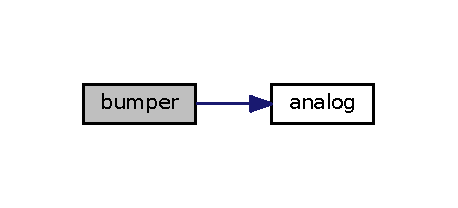
\includegraphics[width=220pt]{firmware_2lib__rwp_8c_a6368ba2819f669bf17962d89b3fca203_cgraph}
\end{center}
\end{figure}


\hypertarget{firmware_2lib__rwp_8c_a9032e2468648895fa936f08f6a831bf9}{\index{firmware/lib\-\_\-rwp.\-c@{firmware/lib\-\_\-rwp.\-c}!drive@{drive}}
\index{drive@{drive}!firmware/lib_rwp.c@{firmware/lib\-\_\-rwp.\-c}}
\subsubsection[{drive}]{\setlength{\rightskip}{0pt plus 5cm}void drive (
\begin{DoxyParamCaption}
\item[{int}]{trans\-\_\-vel, }
\item[{int}]{rot\-\_\-vel}
\end{DoxyParamCaption}
)}}\label{firmware_2lib__rwp_8c_a9032e2468648895fa936f08f6a831bf9}


Here is the call graph for this function\-:
\nopagebreak
\begin{figure}[H]
\begin{center}
\leavevmode
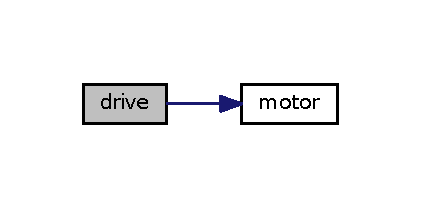
\includegraphics[width=202pt]{firmware_2lib__rwp_8c_a9032e2468648895fa936f08f6a831bf9_cgraph}
\end{center}
\end{figure}


\hypertarget{firmware_2lib__rwp_8c_adac0e25b6c0b34901f454931a366bf51}{\index{firmware/lib\-\_\-rwp.\-c@{firmware/lib\-\_\-rwp.\-c}!init\-\_\-motors@{init\-\_\-motors}}
\index{init\-\_\-motors@{init\-\_\-motors}!firmware/lib_rwp.c@{firmware/lib\-\_\-rwp.\-c}}
\subsubsection[{init\-\_\-motors}]{\setlength{\rightskip}{0pt plus 5cm}int init\-\_\-motors (
\begin{DoxyParamCaption}
{}
\end{DoxyParamCaption}
)}}\label{firmware_2lib__rwp_8c_adac0e25b6c0b34901f454931a366bf51}
\hypertarget{firmware_2lib__rwp_8c_a0bcda6b2106a42058fe25734f7b6efc0}{\index{firmware/lib\-\_\-rwp.\-c@{firmware/lib\-\_\-rwp.\-c}!ir\-\_\-detect@{ir\-\_\-detect}}
\index{ir\-\_\-detect@{ir\-\_\-detect}!firmware/lib_rwp.c@{firmware/lib\-\_\-rwp.\-c}}
\subsubsection[{ir\-\_\-detect}]{\setlength{\rightskip}{0pt plus 5cm}int ir\-\_\-detect (
\begin{DoxyParamCaption}
{}
\end{DoxyParamCaption}
)}}\label{firmware_2lib__rwp_8c_a0bcda6b2106a42058fe25734f7b6efc0}


Here is the call graph for this function\-:
\nopagebreak
\begin{figure}[H]
\begin{center}
\leavevmode
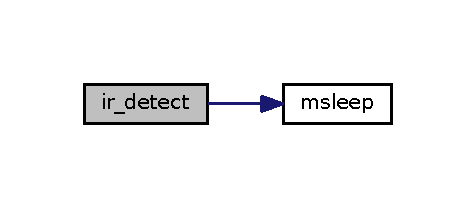
\includegraphics[width=228pt]{firmware_2lib__rwp_8c_a0bcda6b2106a42058fe25734f7b6efc0_cgraph}
\end{center}
\end{figure}


\hypertarget{firmware_2lib__rwp_8c_a49fe73be96a0657e6a3ea6669cdc9f25}{\index{firmware/lib\-\_\-rwp.\-c@{firmware/lib\-\_\-rwp.\-c}!left\-\_\-shaft@{left\-\_\-shaft}}
\index{left\-\_\-shaft@{left\-\_\-shaft}!firmware/lib_rwp.c@{firmware/lib\-\_\-rwp.\-c}}
\subsubsection[{left\-\_\-shaft}]{\setlength{\rightskip}{0pt plus 5cm}int left\-\_\-shaft (
\begin{DoxyParamCaption}
{}
\end{DoxyParamCaption}
)}}\label{firmware_2lib__rwp_8c_a49fe73be96a0657e6a3ea6669cdc9f25}
\hypertarget{firmware_2lib__rwp_8c_a759cd6a2d214a5b16d6e01d114385039}{\index{firmware/lib\-\_\-rwp.\-c@{firmware/lib\-\_\-rwp.\-c}!right\-\_\-shaft@{right\-\_\-shaft}}
\index{right\-\_\-shaft@{right\-\_\-shaft}!firmware/lib_rwp.c@{firmware/lib\-\_\-rwp.\-c}}
\subsubsection[{right\-\_\-shaft}]{\setlength{\rightskip}{0pt plus 5cm}int right\-\_\-shaft (
\begin{DoxyParamCaption}
{}
\end{DoxyParamCaption}
)}}\label{firmware_2lib__rwp_8c_a759cd6a2d214a5b16d6e01d114385039}
\hypertarget{firmware_2lib__rwp_8c_a8c528baf37154d347366083f0f816846}{\index{firmware/lib\-\_\-rwp.\-c@{firmware/lib\-\_\-rwp.\-c}!stop@{stop}}
\index{stop@{stop}!firmware/lib_rwp.c@{firmware/lib\-\_\-rwp.\-c}}
\subsubsection[{stop}]{\setlength{\rightskip}{0pt plus 5cm}void stop (
\begin{DoxyParamCaption}
{}
\end{DoxyParamCaption}
)}}\label{firmware_2lib__rwp_8c_a8c528baf37154d347366083f0f816846}


\subsection{Variable Documentation}
\hypertarget{firmware_2lib__rwp_8c_a40bc49694db9b112049f8a604d1a0b5b}{\index{firmware/lib\-\_\-rwp.\-c@{firmware/lib\-\_\-rwp.\-c}!dir\-\_\-mask@{dir\-\_\-mask}}
\index{dir\-\_\-mask@{dir\-\_\-mask}!firmware/lib_rwp.c@{firmware/lib\-\_\-rwp.\-c}}
\subsubsection[{dir\-\_\-mask}]{\setlength{\rightskip}{0pt plus 5cm}int dir\-\_\-mask\mbox{[}2\mbox{]} = \{0b00010000, 0b00100000\}}}\label{firmware_2lib__rwp_8c_a40bc49694db9b112049f8a604d1a0b5b}
\hypertarget{firmware_2lib__rwp_8c_ab98f1128461d00f21e140e84a06b1ecb}{\index{firmware/lib\-\_\-rwp.\-c@{firmware/lib\-\_\-rwp.\-c}!init\-\_\-motors\-\_\-dummy@{init\-\_\-motors\-\_\-dummy}}
\index{init\-\_\-motors\-\_\-dummy@{init\-\_\-motors\-\_\-dummy}!firmware/lib_rwp.c@{firmware/lib\-\_\-rwp.\-c}}
\subsubsection[{init\-\_\-motors\-\_\-dummy}]{\setlength{\rightskip}{0pt plus 5cm}int init\-\_\-motors\-\_\-dummy = {\bf init\-\_\-motors}()}}\label{firmware_2lib__rwp_8c_ab98f1128461d00f21e140e84a06b1ecb}
\hypertarget{firmware_2lib__rwp_8c_a1793fe255c482750301ca7e5ea57874d}{\index{firmware/lib\-\_\-rwp.\-c@{firmware/lib\-\_\-rwp.\-c}!microphone@{microphone}}
\index{microphone@{microphone}!firmware/lib_rwp.c@{firmware/lib\-\_\-rwp.\-c}}
\subsubsection[{microphone}]{\setlength{\rightskip}{0pt plus 5cm}int microphone = 2}}\label{firmware_2lib__rwp_8c_a1793fe255c482750301ca7e5ea57874d}
\hypertarget{firmware_2lib__rwp_8c_a80003173b2b20936eebe10521f94b503}{\index{firmware/lib\-\_\-rwp.\-c@{firmware/lib\-\_\-rwp.\-c}!photo\-\_\-left@{photo\-\_\-left}}
\index{photo\-\_\-left@{photo\-\_\-left}!firmware/lib_rwp.c@{firmware/lib\-\_\-rwp.\-c}}
\subsubsection[{photo\-\_\-left}]{\setlength{\rightskip}{0pt plus 5cm}int photo\-\_\-left = 1}}\label{firmware_2lib__rwp_8c_a80003173b2b20936eebe10521f94b503}
\hypertarget{firmware_2lib__rwp_8c_abf8c764cb5f5289ee3688871415dd737}{\index{firmware/lib\-\_\-rwp.\-c@{firmware/lib\-\_\-rwp.\-c}!photo\-\_\-right@{photo\-\_\-right}}
\index{photo\-\_\-right@{photo\-\_\-right}!firmware/lib_rwp.c@{firmware/lib\-\_\-rwp.\-c}}
\subsubsection[{photo\-\_\-right}]{\setlength{\rightskip}{0pt plus 5cm}int photo\-\_\-right = 0}}\label{firmware_2lib__rwp_8c_abf8c764cb5f5289ee3688871415dd737}
\hypertarget{firmware_2lib__rwp_8c_af583a71fc7eabd31426624437cd1a8f3}{\index{firmware/lib\-\_\-rwp.\-c@{firmware/lib\-\_\-rwp.\-c}!pwm\-\_\-mask@{pwm\-\_\-mask}}
\index{pwm\-\_\-mask@{pwm\-\_\-mask}!firmware/lib_rwp.c@{firmware/lib\-\_\-rwp.\-c}}
\subsubsection[{pwm\-\_\-mask}]{\setlength{\rightskip}{0pt plus 5cm}int pwm\-\_\-mask\mbox{[}2\mbox{]} = \{0b01000000, 0b00100000\}}}\label{firmware_2lib__rwp_8c_af583a71fc7eabd31426624437cd1a8f3}
\hypertarget{firmware_2lib__rwp_8c_aadb76e04ceadfab884568976b02ccb95}{\index{firmware/lib\-\_\-rwp.\-c@{firmware/lib\-\_\-rwp.\-c}!T\-O\-Cx@{T\-O\-Cx}}
\index{T\-O\-Cx@{T\-O\-Cx}!firmware/lib_rwp.c@{firmware/lib\-\_\-rwp.\-c}}
\subsubsection[{T\-O\-Cx}]{\setlength{\rightskip}{0pt plus 5cm}int T\-O\-Cx\mbox{[}2\mbox{]} = \{0x1018, 0x101\-A\}}}\label{firmware_2lib__rwp_8c_aadb76e04ceadfab884568976b02ccb95}

\hypertarget{menu_8c}{\section{/root/\-Desktop/rug-\/warrior/libs/base/menu.c File Reference}
\label{menu_8c}\index{/root/\-Desktop/rug-\/warrior/libs/base/menu.\-c@{/root/\-Desktop/rug-\/warrior/libs/base/menu.\-c}}
}
\subsection*{Macros}
\begin{DoxyCompactItemize}
\item 
\#define \hyperlink{menu_8c_a56e7715cc82d0a653439627059cfa7e6}{N\-E\-I\-T\-H\-E\-R\-\_\-\-B}~0
\item 
\#define \hyperlink{menu_8c_ab01ab67b3216b90828b17a031ab4aa35}{C\-H\-O\-O\-S\-E\-\_\-\-B}~1
\item 
\#define \hyperlink{menu_8c_a77f4f240759db674b4fdd3614c2d0ad0}{E\-S\-C\-A\-P\-E\-\_\-\-B}~2
\item 
\#define \hyperlink{menu_8c_ac3a317b74a9e22f2000ef8eb57ae0d0c}{U\-P\-\_\-\-B}~3
\item 
\#define \hyperlink{menu_8c_a6b23a11f921b05f4ccc12dab38e4b7fe}{D\-O\-W\-N\-\_\-\-B}~4
\item 
\#define \hyperlink{menu_8c_abfa3e36fb028ae048c2d34b0f5d0e265}{C\-Y\-C\-L\-E\-\_\-\-B}~5
\end{DoxyCompactItemize}
\subsection*{Functions}
\begin{DoxyCompactItemize}
\item 
int \hyperlink{menu_8c_ade420648ad5e270eb49e76bc71fcb203}{chosen\-\_\-button} ()
\item 
int \hyperlink{menu_8c_aad05720d81aee6fe57273df91d1206d1}{wait\-\_\-button} (int i)
\item 
int \hyperlink{menu_8c_aa7168d52d66264c671f6470176856fd1}{select\-\_\-int\-\_\-value} (char s\mbox{[}$\,$\mbox{]}, int min\-\_\-val, int max\-\_\-val)
\item 
float \hyperlink{menu_8c_a0a37e579c94982ce5cf6d631464f96ea}{select\-\_\-float\-\_\-value} (char s\mbox{[}$\,$\mbox{]}, float min\-\_\-val, float max\-\_\-val)
\item 
int \hyperlink{menu_8c_a1b08ad6fdc5215cef1a76e23f309dae1}{select\-\_\-string} (char choices\mbox{[}$\,$\mbox{]}\mbox{[}$\,$\mbox{]}, int n)
\end{DoxyCompactItemize}


\subsection{Macro Definition Documentation}
\hypertarget{menu_8c_ab01ab67b3216b90828b17a031ab4aa35}{\index{menu.\-c@{menu.\-c}!C\-H\-O\-O\-S\-E\-\_\-\-B@{C\-H\-O\-O\-S\-E\-\_\-\-B}}
\index{C\-H\-O\-O\-S\-E\-\_\-\-B@{C\-H\-O\-O\-S\-E\-\_\-\-B}!menu.c@{menu.\-c}}
\subsubsection[{C\-H\-O\-O\-S\-E\-\_\-\-B}]{\setlength{\rightskip}{0pt plus 5cm}\#define C\-H\-O\-O\-S\-E\-\_\-\-B~1}}\label{menu_8c_ab01ab67b3216b90828b17a031ab4aa35}
\hypertarget{menu_8c_abfa3e36fb028ae048c2d34b0f5d0e265}{\index{menu.\-c@{menu.\-c}!C\-Y\-C\-L\-E\-\_\-\-B@{C\-Y\-C\-L\-E\-\_\-\-B}}
\index{C\-Y\-C\-L\-E\-\_\-\-B@{C\-Y\-C\-L\-E\-\_\-\-B}!menu.c@{menu.\-c}}
\subsubsection[{C\-Y\-C\-L\-E\-\_\-\-B}]{\setlength{\rightskip}{0pt plus 5cm}\#define C\-Y\-C\-L\-E\-\_\-\-B~5}}\label{menu_8c_abfa3e36fb028ae048c2d34b0f5d0e265}
\hypertarget{menu_8c_a6b23a11f921b05f4ccc12dab38e4b7fe}{\index{menu.\-c@{menu.\-c}!D\-O\-W\-N\-\_\-\-B@{D\-O\-W\-N\-\_\-\-B}}
\index{D\-O\-W\-N\-\_\-\-B@{D\-O\-W\-N\-\_\-\-B}!menu.c@{menu.\-c}}
\subsubsection[{D\-O\-W\-N\-\_\-\-B}]{\setlength{\rightskip}{0pt plus 5cm}\#define D\-O\-W\-N\-\_\-\-B~4}}\label{menu_8c_a6b23a11f921b05f4ccc12dab38e4b7fe}
\hypertarget{menu_8c_a77f4f240759db674b4fdd3614c2d0ad0}{\index{menu.\-c@{menu.\-c}!E\-S\-C\-A\-P\-E\-\_\-\-B@{E\-S\-C\-A\-P\-E\-\_\-\-B}}
\index{E\-S\-C\-A\-P\-E\-\_\-\-B@{E\-S\-C\-A\-P\-E\-\_\-\-B}!menu.c@{menu.\-c}}
\subsubsection[{E\-S\-C\-A\-P\-E\-\_\-\-B}]{\setlength{\rightskip}{0pt plus 5cm}\#define E\-S\-C\-A\-P\-E\-\_\-\-B~2}}\label{menu_8c_a77f4f240759db674b4fdd3614c2d0ad0}
\hypertarget{menu_8c_a56e7715cc82d0a653439627059cfa7e6}{\index{menu.\-c@{menu.\-c}!N\-E\-I\-T\-H\-E\-R\-\_\-\-B@{N\-E\-I\-T\-H\-E\-R\-\_\-\-B}}
\index{N\-E\-I\-T\-H\-E\-R\-\_\-\-B@{N\-E\-I\-T\-H\-E\-R\-\_\-\-B}!menu.c@{menu.\-c}}
\subsubsection[{N\-E\-I\-T\-H\-E\-R\-\_\-\-B}]{\setlength{\rightskip}{0pt plus 5cm}\#define N\-E\-I\-T\-H\-E\-R\-\_\-\-B~0}}\label{menu_8c_a56e7715cc82d0a653439627059cfa7e6}
\hypertarget{menu_8c_ac3a317b74a9e22f2000ef8eb57ae0d0c}{\index{menu.\-c@{menu.\-c}!U\-P\-\_\-\-B@{U\-P\-\_\-\-B}}
\index{U\-P\-\_\-\-B@{U\-P\-\_\-\-B}!menu.c@{menu.\-c}}
\subsubsection[{U\-P\-\_\-\-B}]{\setlength{\rightskip}{0pt plus 5cm}\#define U\-P\-\_\-\-B~3}}\label{menu_8c_ac3a317b74a9e22f2000ef8eb57ae0d0c}


\subsection{Function Documentation}
\hypertarget{menu_8c_ade420648ad5e270eb49e76bc71fcb203}{\index{menu.\-c@{menu.\-c}!chosen\-\_\-button@{chosen\-\_\-button}}
\index{chosen\-\_\-button@{chosen\-\_\-button}!menu.c@{menu.\-c}}
\subsubsection[{chosen\-\_\-button}]{\setlength{\rightskip}{0pt plus 5cm}int chosen\-\_\-button (
\begin{DoxyParamCaption}
{}
\end{DoxyParamCaption}
)}}\label{menu_8c_ade420648ad5e270eb49e76bc71fcb203}


Here is the call graph for this function\-:
\nopagebreak
\begin{figure}[H]
\begin{center}
\leavevmode
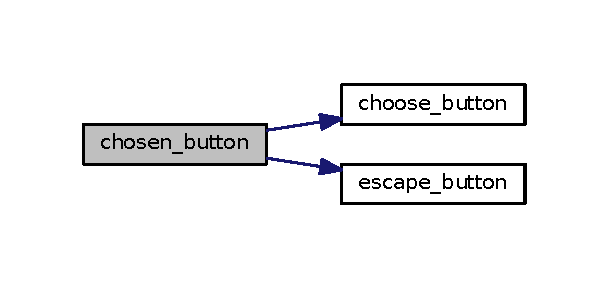
\includegraphics[width=292pt]{menu_8c_ade420648ad5e270eb49e76bc71fcb203_cgraph}
\end{center}
\end{figure}




Here is the caller graph for this function\-:
\nopagebreak
\begin{figure}[H]
\begin{center}
\leavevmode
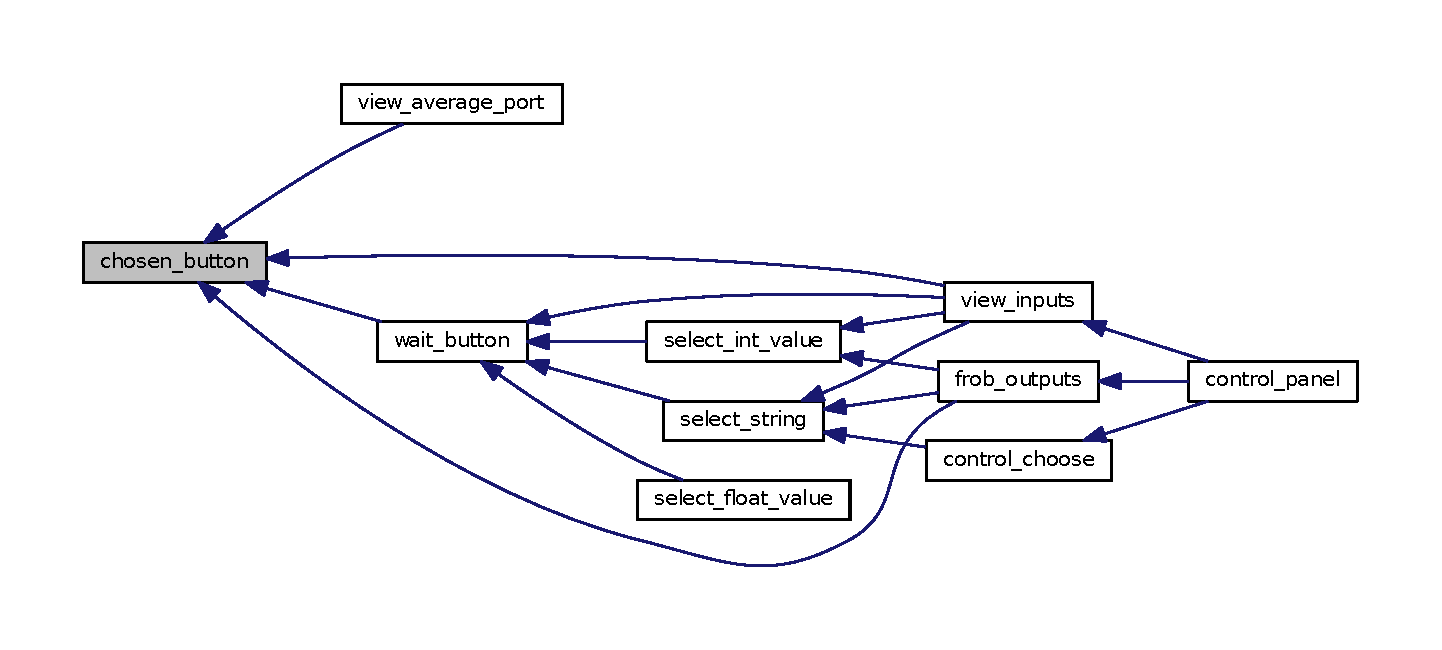
\includegraphics[width=350pt]{menu_8c_ade420648ad5e270eb49e76bc71fcb203_icgraph}
\end{center}
\end{figure}


\hypertarget{menu_8c_a0a37e579c94982ce5cf6d631464f96ea}{\index{menu.\-c@{menu.\-c}!select\-\_\-float\-\_\-value@{select\-\_\-float\-\_\-value}}
\index{select\-\_\-float\-\_\-value@{select\-\_\-float\-\_\-value}!menu.c@{menu.\-c}}
\subsubsection[{select\-\_\-float\-\_\-value}]{\setlength{\rightskip}{0pt plus 5cm}float select\-\_\-float\-\_\-value (
\begin{DoxyParamCaption}
\item[{char}]{s\mbox{[}$\,$\mbox{]}, }
\item[{float}]{min\-\_\-val, }
\item[{float}]{max\-\_\-val}
\end{DoxyParamCaption}
)}}\label{menu_8c_a0a37e579c94982ce5cf6d631464f96ea}
-\/1 means escape -- do not reset value 

Here is the call graph for this function\-:
\nopagebreak
\begin{figure}[H]
\begin{center}
\leavevmode
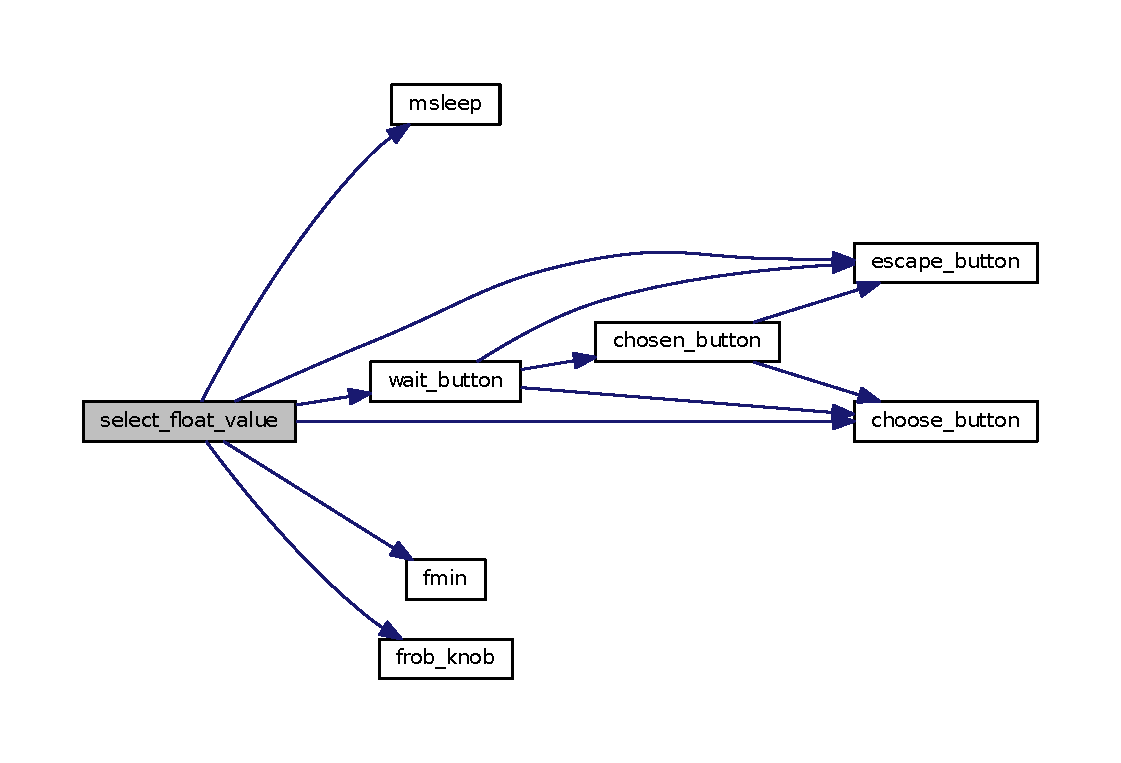
\includegraphics[width=350pt]{menu_8c_a0a37e579c94982ce5cf6d631464f96ea_cgraph}
\end{center}
\end{figure}


\hypertarget{menu_8c_aa7168d52d66264c671f6470176856fd1}{\index{menu.\-c@{menu.\-c}!select\-\_\-int\-\_\-value@{select\-\_\-int\-\_\-value}}
\index{select\-\_\-int\-\_\-value@{select\-\_\-int\-\_\-value}!menu.c@{menu.\-c}}
\subsubsection[{select\-\_\-int\-\_\-value}]{\setlength{\rightskip}{0pt plus 5cm}int select\-\_\-int\-\_\-value (
\begin{DoxyParamCaption}
\item[{char}]{s\mbox{[}$\,$\mbox{]}, }
\item[{int}]{min\-\_\-val, }
\item[{int}]{max\-\_\-val}
\end{DoxyParamCaption}
)}}\label{menu_8c_aa7168d52d66264c671f6470176856fd1}
-\/1 means escape -- do not reset value 

Here is the call graph for this function\-:
\nopagebreak
\begin{figure}[H]
\begin{center}
\leavevmode
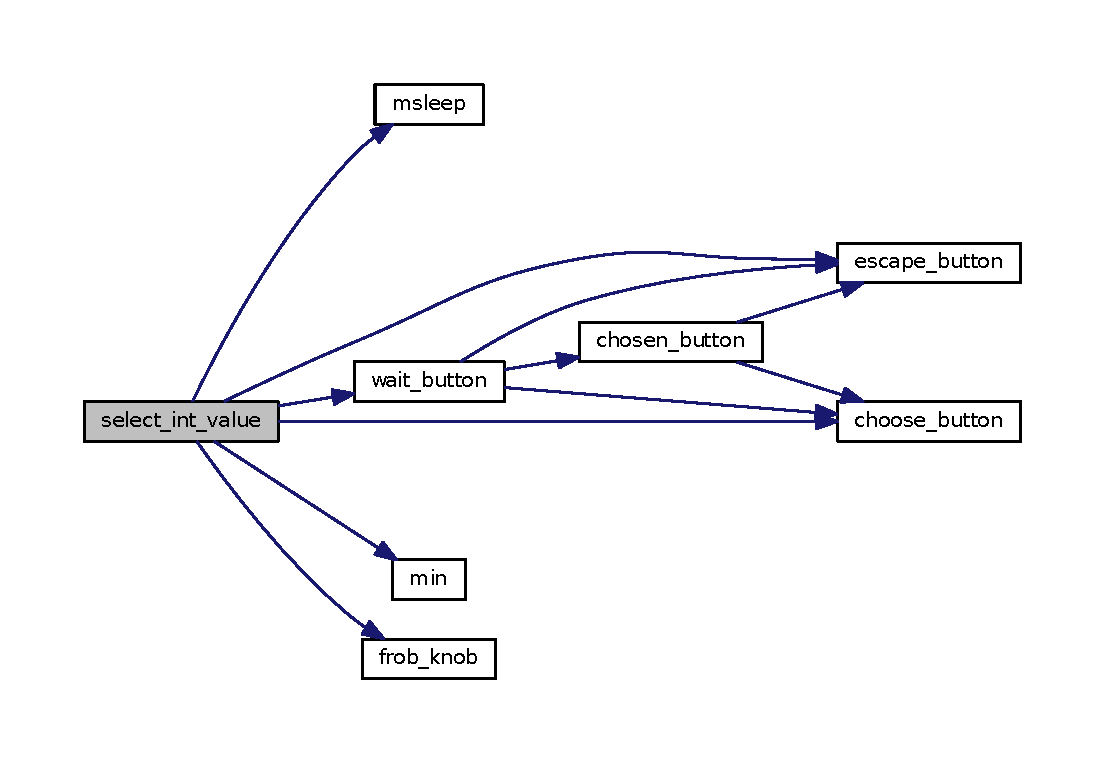
\includegraphics[width=350pt]{menu_8c_aa7168d52d66264c671f6470176856fd1_cgraph}
\end{center}
\end{figure}




Here is the caller graph for this function\-:
\nopagebreak
\begin{figure}[H]
\begin{center}
\leavevmode
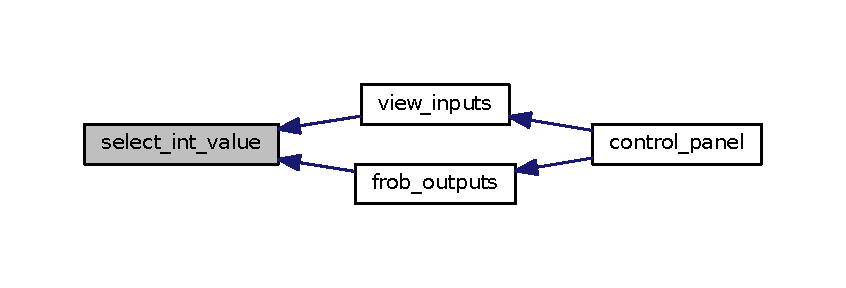
\includegraphics[width=350pt]{menu_8c_aa7168d52d66264c671f6470176856fd1_icgraph}
\end{center}
\end{figure}


\hypertarget{menu_8c_a1b08ad6fdc5215cef1a76e23f309dae1}{\index{menu.\-c@{menu.\-c}!select\-\_\-string@{select\-\_\-string}}
\index{select\-\_\-string@{select\-\_\-string}!menu.c@{menu.\-c}}
\subsubsection[{select\-\_\-string}]{\setlength{\rightskip}{0pt plus 5cm}int select\-\_\-string (
\begin{DoxyParamCaption}
\item[{char}]{choices\mbox{[}$\,$\mbox{]}\mbox{[}$\,$\mbox{]}, }
\item[{int}]{n}
\end{DoxyParamCaption}
)}}\label{menu_8c_a1b08ad6fdc5215cef1a76e23f309dae1}


Here is the call graph for this function\-:
\nopagebreak
\begin{figure}[H]
\begin{center}
\leavevmode
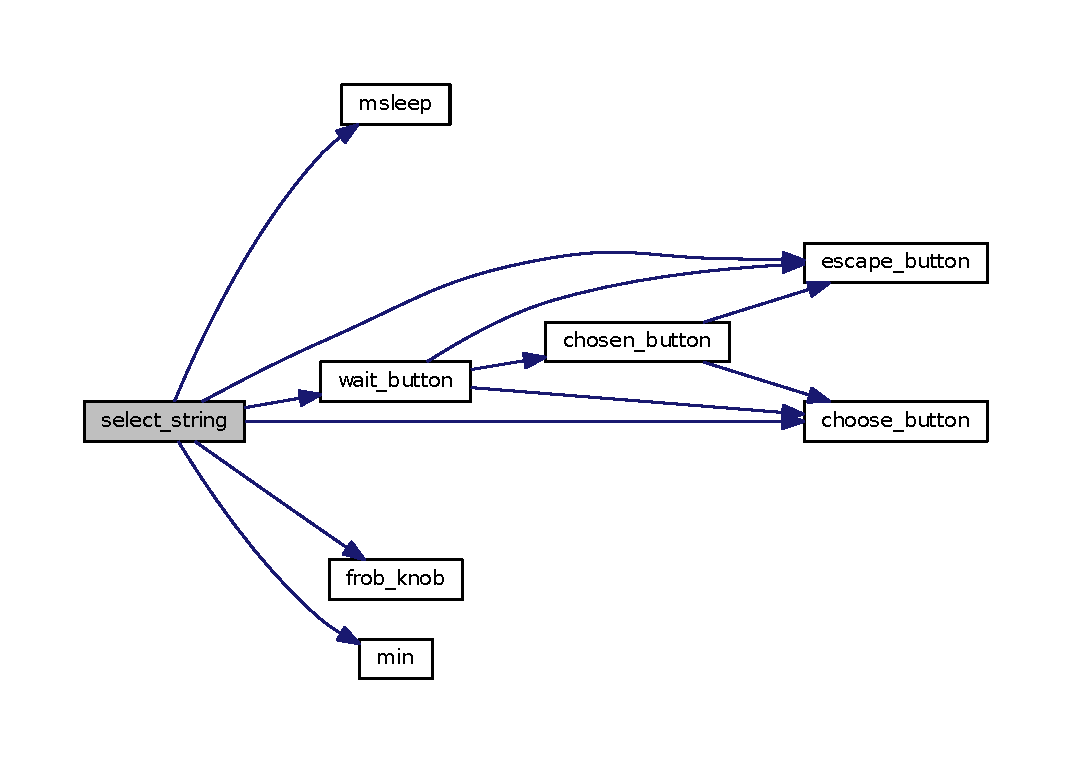
\includegraphics[width=350pt]{menu_8c_a1b08ad6fdc5215cef1a76e23f309dae1_cgraph}
\end{center}
\end{figure}




Here is the caller graph for this function\-:
\nopagebreak
\begin{figure}[H]
\begin{center}
\leavevmode
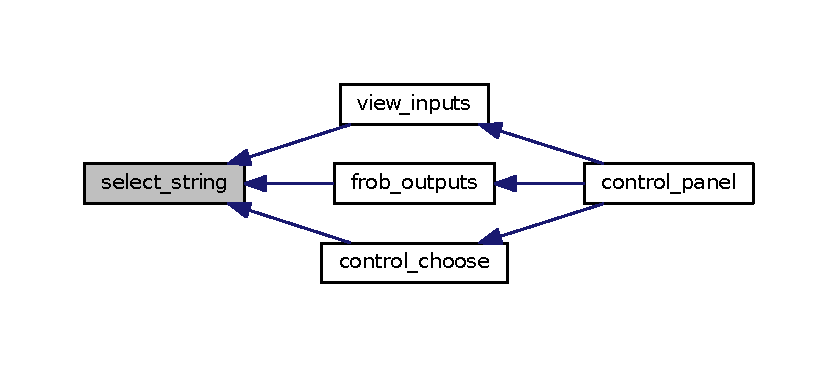
\includegraphics[width=350pt]{menu_8c_a1b08ad6fdc5215cef1a76e23f309dae1_icgraph}
\end{center}
\end{figure}


\hypertarget{menu_8c_aad05720d81aee6fe57273df91d1206d1}{\index{menu.\-c@{menu.\-c}!wait\-\_\-button@{wait\-\_\-button}}
\index{wait\-\_\-button@{wait\-\_\-button}!menu.c@{menu.\-c}}
\subsubsection[{wait\-\_\-button}]{\setlength{\rightskip}{0pt plus 5cm}int wait\-\_\-button (
\begin{DoxyParamCaption}
\item[{int}]{i}
\end{DoxyParamCaption}
)}}\label{menu_8c_aad05720d81aee6fe57273df91d1206d1}


Here is the call graph for this function\-:
\nopagebreak
\begin{figure}[H]
\begin{center}
\leavevmode
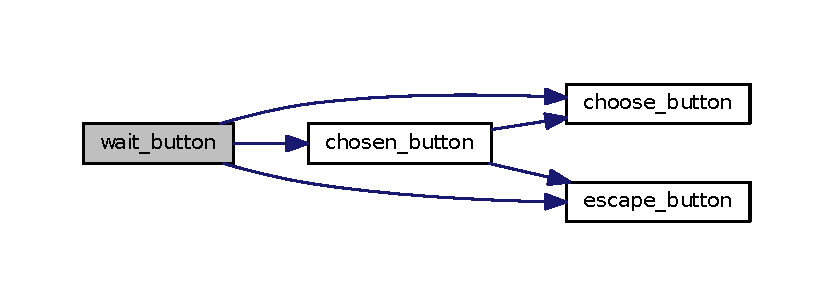
\includegraphics[width=350pt]{menu_8c_aad05720d81aee6fe57273df91d1206d1_cgraph}
\end{center}
\end{figure}




Here is the caller graph for this function\-:
\nopagebreak
\begin{figure}[H]
\begin{center}
\leavevmode
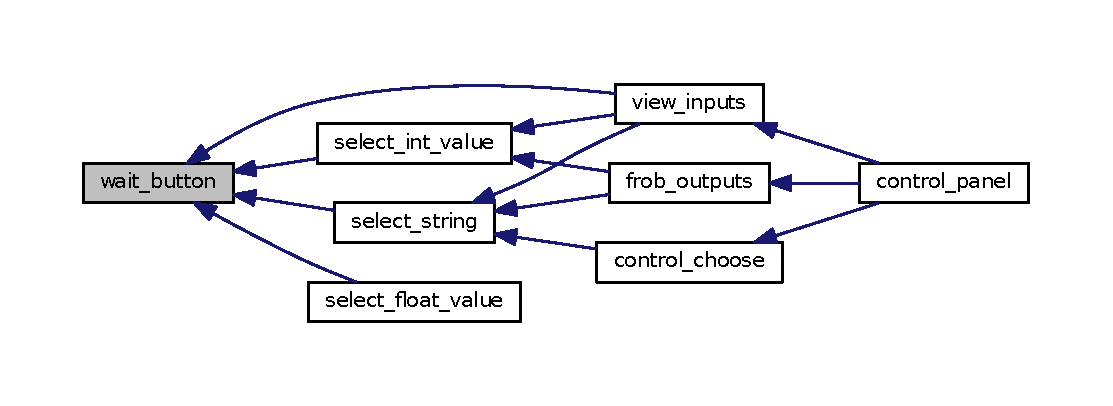
\includegraphics[width=350pt]{menu_8c_aad05720d81aee6fe57273df91d1206d1_icgraph}
\end{center}
\end{figure}



\hypertarget{r22__ir_8c}{\section{/root/\-Desktop/ic\-\_\-linux\-\_\-3.1/libs/base/r22\-\_\-ir.c File Reference}
\label{r22__ir_8c}\index{/root/\-Desktop/ic\-\_\-linux\-\_\-3.\-1/libs/base/r22\-\_\-ir.\-c@{/root/\-Desktop/ic\-\_\-linux\-\_\-3.\-1/libs/base/r22\-\_\-ir.\-c}}
}
\subsection*{Functions}
\begin{DoxyCompactItemize}
\item 
void \hyperlink{r22__ir_8c_a211f904daceebd1873f7aae7b3f8c7f3}{ir\-\_\-transmit\-\_\-on} ()
\item 
void \hyperlink{r22__ir_8c_a66be7ce57773daca4a1555e3cad91181}{ir\-\_\-transmit\-\_\-off} ()
\item 
void \hyperlink{r22__ir_8c_a9a71de6531510ddb852d51f35d65af38}{set\-\_\-ir\-\_\-transmit\-\_\-period} (int period)
\item 
void \hyperlink{r22__ir_8c_ae2de6d8cad46252db6539a1774f2cb15}{set\-\_\-ir\-\_\-transmit\-\_\-frequency} (int \hyperlink{cof_8c_af900396d7b72ff2a7002e8befe8cf8f1}{f})
\item 
void \hyperlink{r22__ir_8c_a1526c7a46d27ac5f8c5b5e0a97e43c3a}{set\-\_\-ir\-\_\-receive\-\_\-period} (int period)
\item 
void \hyperlink{r22__ir_8c_a096502726937deca6fbae7dbf2b95469}{set\-\_\-ir\-\_\-receive\-\_\-frequency} (int \hyperlink{cof_8c_af900396d7b72ff2a7002e8befe8cf8f1}{f})
\item 
int \hyperlink{r22__ir_8c_af3172b03a9f77e67f161ca8fb56b5eda}{ir\-\_\-counts} (int p)
\item 
void \hyperlink{r22__ir_8c_a5086e028f715d9af04cab61f87cbd94c}{ir\-\_\-receive\-\_\-off} ()
\item 
void \hyperlink{r22__ir_8c_ac45a3edcdb98be42ee7db755a12e0b46}{ir\-\_\-receive\-\_\-on} ()
\end{DoxyCompactItemize}


\subsection{Function Documentation}
\hypertarget{r22__ir_8c_af3172b03a9f77e67f161ca8fb56b5eda}{\index{r22\-\_\-ir.\-c@{r22\-\_\-ir.\-c}!ir\-\_\-counts@{ir\-\_\-counts}}
\index{ir\-\_\-counts@{ir\-\_\-counts}!r22_ir.c@{r22\-\_\-ir.\-c}}
\subsubsection[{ir\-\_\-counts}]{\setlength{\rightskip}{0pt plus 5cm}int ir\-\_\-counts (
\begin{DoxyParamCaption}
\item[{int}]{p}
\end{DoxyParamCaption}
)}}\label{r22__ir_8c_af3172b03a9f77e67f161ca8fb56b5eda}
\hypertarget{r22__ir_8c_a5086e028f715d9af04cab61f87cbd94c}{\index{r22\-\_\-ir.\-c@{r22\-\_\-ir.\-c}!ir\-\_\-receive\-\_\-off@{ir\-\_\-receive\-\_\-off}}
\index{ir\-\_\-receive\-\_\-off@{ir\-\_\-receive\-\_\-off}!r22_ir.c@{r22\-\_\-ir.\-c}}
\subsubsection[{ir\-\_\-receive\-\_\-off}]{\setlength{\rightskip}{0pt plus 5cm}void ir\-\_\-receive\-\_\-off (
\begin{DoxyParamCaption}
{}
\end{DoxyParamCaption}
)}}\label{r22__ir_8c_a5086e028f715d9af04cab61f87cbd94c}
\hypertarget{r22__ir_8c_ac45a3edcdb98be42ee7db755a12e0b46}{\index{r22\-\_\-ir.\-c@{r22\-\_\-ir.\-c}!ir\-\_\-receive\-\_\-on@{ir\-\_\-receive\-\_\-on}}
\index{ir\-\_\-receive\-\_\-on@{ir\-\_\-receive\-\_\-on}!r22_ir.c@{r22\-\_\-ir.\-c}}
\subsubsection[{ir\-\_\-receive\-\_\-on}]{\setlength{\rightskip}{0pt plus 5cm}void ir\-\_\-receive\-\_\-on (
\begin{DoxyParamCaption}
{}
\end{DoxyParamCaption}
)}}\label{r22__ir_8c_ac45a3edcdb98be42ee7db755a12e0b46}
\hypertarget{r22__ir_8c_a66be7ce57773daca4a1555e3cad91181}{\index{r22\-\_\-ir.\-c@{r22\-\_\-ir.\-c}!ir\-\_\-transmit\-\_\-off@{ir\-\_\-transmit\-\_\-off}}
\index{ir\-\_\-transmit\-\_\-off@{ir\-\_\-transmit\-\_\-off}!r22_ir.c@{r22\-\_\-ir.\-c}}
\subsubsection[{ir\-\_\-transmit\-\_\-off}]{\setlength{\rightskip}{0pt plus 5cm}void ir\-\_\-transmit\-\_\-off (
\begin{DoxyParamCaption}
{}
\end{DoxyParamCaption}
)}}\label{r22__ir_8c_a66be7ce57773daca4a1555e3cad91181}
\hypertarget{r22__ir_8c_a211f904daceebd1873f7aae7b3f8c7f3}{\index{r22\-\_\-ir.\-c@{r22\-\_\-ir.\-c}!ir\-\_\-transmit\-\_\-on@{ir\-\_\-transmit\-\_\-on}}
\index{ir\-\_\-transmit\-\_\-on@{ir\-\_\-transmit\-\_\-on}!r22_ir.c@{r22\-\_\-ir.\-c}}
\subsubsection[{ir\-\_\-transmit\-\_\-on}]{\setlength{\rightskip}{0pt plus 5cm}void ir\-\_\-transmit\-\_\-on (
\begin{DoxyParamCaption}
{}
\end{DoxyParamCaption}
)}}\label{r22__ir_8c_a211f904daceebd1873f7aae7b3f8c7f3}
\hypertarget{r22__ir_8c_a096502726937deca6fbae7dbf2b95469}{\index{r22\-\_\-ir.\-c@{r22\-\_\-ir.\-c}!set\-\_\-ir\-\_\-receive\-\_\-frequency@{set\-\_\-ir\-\_\-receive\-\_\-frequency}}
\index{set\-\_\-ir\-\_\-receive\-\_\-frequency@{set\-\_\-ir\-\_\-receive\-\_\-frequency}!r22_ir.c@{r22\-\_\-ir.\-c}}
\subsubsection[{set\-\_\-ir\-\_\-receive\-\_\-frequency}]{\setlength{\rightskip}{0pt plus 5cm}void set\-\_\-ir\-\_\-receive\-\_\-frequency (
\begin{DoxyParamCaption}
\item[{int}]{f}
\end{DoxyParamCaption}
)}}\label{r22__ir_8c_a096502726937deca6fbae7dbf2b95469}
\hypertarget{r22__ir_8c_a1526c7a46d27ac5f8c5b5e0a97e43c3a}{\index{r22\-\_\-ir.\-c@{r22\-\_\-ir.\-c}!set\-\_\-ir\-\_\-receive\-\_\-period@{set\-\_\-ir\-\_\-receive\-\_\-period}}
\index{set\-\_\-ir\-\_\-receive\-\_\-period@{set\-\_\-ir\-\_\-receive\-\_\-period}!r22_ir.c@{r22\-\_\-ir.\-c}}
\subsubsection[{set\-\_\-ir\-\_\-receive\-\_\-period}]{\setlength{\rightskip}{0pt plus 5cm}void set\-\_\-ir\-\_\-receive\-\_\-period (
\begin{DoxyParamCaption}
\item[{int}]{period}
\end{DoxyParamCaption}
)}}\label{r22__ir_8c_a1526c7a46d27ac5f8c5b5e0a97e43c3a}
\hypertarget{r22__ir_8c_ae2de6d8cad46252db6539a1774f2cb15}{\index{r22\-\_\-ir.\-c@{r22\-\_\-ir.\-c}!set\-\_\-ir\-\_\-transmit\-\_\-frequency@{set\-\_\-ir\-\_\-transmit\-\_\-frequency}}
\index{set\-\_\-ir\-\_\-transmit\-\_\-frequency@{set\-\_\-ir\-\_\-transmit\-\_\-frequency}!r22_ir.c@{r22\-\_\-ir.\-c}}
\subsubsection[{set\-\_\-ir\-\_\-transmit\-\_\-frequency}]{\setlength{\rightskip}{0pt plus 5cm}void set\-\_\-ir\-\_\-transmit\-\_\-frequency (
\begin{DoxyParamCaption}
\item[{int}]{f}
\end{DoxyParamCaption}
)}}\label{r22__ir_8c_ae2de6d8cad46252db6539a1774f2cb15}
\hypertarget{r22__ir_8c_a9a71de6531510ddb852d51f35d65af38}{\index{r22\-\_\-ir.\-c@{r22\-\_\-ir.\-c}!set\-\_\-ir\-\_\-transmit\-\_\-period@{set\-\_\-ir\-\_\-transmit\-\_\-period}}
\index{set\-\_\-ir\-\_\-transmit\-\_\-period@{set\-\_\-ir\-\_\-transmit\-\_\-period}!r22_ir.c@{r22\-\_\-ir.\-c}}
\subsubsection[{set\-\_\-ir\-\_\-transmit\-\_\-period}]{\setlength{\rightskip}{0pt plus 5cm}void set\-\_\-ir\-\_\-transmit\-\_\-period (
\begin{DoxyParamCaption}
\item[{int}]{period}
\end{DoxyParamCaption}
)}}\label{r22__ir_8c_a9a71de6531510ddb852d51f35d65af38}

\hypertarget{regdefs_8c}{\section{/root/\-Desktop/rug-\/warrior/libs/base/regdefs.c File Reference}
\label{regdefs_8c}\index{/root/\-Desktop/rug-\/warrior/libs/base/regdefs.\-c@{/root/\-Desktop/rug-\/warrior/libs/base/regdefs.\-c}}
}
\subsection*{Variables}
\begin{DoxyCompactItemize}
\item 
int \hyperlink{regdefs_8c_ad2418a7bce80afb6f10e4db918286882}{port\-\_\-a} = 0x1000
\item 
int \hyperlink{regdefs_8c_a410101f24c9b4159ee85224bb98396d3}{port\-\_\-d} = 0x1008
\item 
int \hyperlink{regdefs_8c_a7f40325aaddc75ec8e13cdd34400047d}{porta} = 0x1000
\item 
int \hyperlink{regdefs_8c_a1fe6b7fb3cb919e9d076355819e249e2}{pioc} = 0x1002
\item 
int \hyperlink{regdefs_8c_a134599483af0c222f05597a818de4ac6}{portc} = 0x1003
\item 
int \hyperlink{regdefs_8c_a98e200bd29fdd78738d3594990c12644}{portb} = 0x1004
\item 
int \hyperlink{regdefs_8c_aaac1d32cb59dab379299c662c57edf71}{portcl} = 0x1005
\item 
int \hyperlink{regdefs_8c_a4c22e0c466f82b9967bde5ee5edc7bac}{ddrc} = 0x1007
\item 
int \hyperlink{regdefs_8c_ab06b67414c7fd0450b0558e5c84067a0}{portd} = 0x1008
\item 
int \hyperlink{regdefs_8c_ac81a75d556d4c4d9e3bad42e790b85a7}{ddrd} = 0x1009
\item 
int \hyperlink{regdefs_8c_a197f6352c6d8dce3ad896c17394e8166}{porte} = 0x100\-A
\item 
int \hyperlink{regdefs_8c_a9182598b2743149800b432c06abdbdad}{cforce} = 0x100\-B
\item 
int \hyperlink{regdefs_8c_ab942e1938408be0e2d7362faec934dc8}{oc1m} = 0x100\-C
\item 
int \hyperlink{regdefs_8c_ac0e1617e9598619e615b19c15e6ca33b}{oc1d} = 0x100\-D
\item 
int \hyperlink{regdefs_8c_a673b9a037f53cc16c3bdfabb095e2828}{tcnt} = 0x100\-E
\item 
int \hyperlink{regdefs_8c_aa403b99859365356e01abc3f7cc14db1}{tic1} = 0x1010
\item 
int \hyperlink{regdefs_8c_ae279a4a5e5350cc06b41d983e2b30c35}{tic2} = 0x1012
\item 
int \hyperlink{regdefs_8c_a59a8146b1d9ba4f77a96599adf0eb5ae}{tic3} = 0x1014
\item 
int \hyperlink{regdefs_8c_a95ea3e9132f8668b35d4bb59fad3c678}{toc1} = 0x1016
\item 
int \hyperlink{regdefs_8c_a4facaea9d0019ee04b45347ad613f174}{toc2} = 0x1018
\item 
int \hyperlink{regdefs_8c_a907efd7230a8f3d5752c896834d42818}{toc3} = 0x101\-A
\item 
int \hyperlink{regdefs_8c_a86ce40895f68ac75060d54104dd31632}{toc4} = 0x101\-C
\item 
int \hyperlink{regdefs_8c_a9c175667fe5da1871a7ed7a4187bd8cb}{toc5} = 0x101\-E
\item 
int \hyperlink{regdefs_8c_a346698dd299e2e8635acd0efc32b6db1}{tctl1} = 0x1020
\item 
int \hyperlink{regdefs_8c_ab04b15b8d404e1d2f44516d73c6664b4}{tctl2} = 0x1021
\item 
int \hyperlink{regdefs_8c_a376ec9a27c1cc1202378bc7e6f261a26}{tmsk1} = 0x1022
\item 
int \hyperlink{regdefs_8c_a5a8c55e10291fbdc4d263c8dfb5f462e}{tflg1} = 0x1023
\item 
int \hyperlink{regdefs_8c_a246ea63e87ff07324cb1f091f74a5f31}{tmsk2} = 0x1024
\item 
int \hyperlink{regdefs_8c_ab3a83e5bdd4249bbc06411dea690a75c}{tflg2} = 0x1025
\item 
int \hyperlink{regdefs_8c_ab87f84af9fc12ac8412454800d71782a}{pactl} = 0x1026
\item 
int \hyperlink{regdefs_8c_a0db11746f5e8d5a3007fa9e635746802}{pacnt} = 0x1027
\item 
int \hyperlink{regdefs_8c_ad4e36089dc2d1e0c4bc8d88cb94eaf65}{spcr} = 0x1028
\item 
int \hyperlink{regdefs_8c_a43a885143f98bf237cc68c65ef3e84f0}{spsr} = 0x1029
\item 
int \hyperlink{regdefs_8c_a3f159ae4e82aa47887d3bc255bf71809}{spdr} = 0x102\-A
\item 
int \hyperlink{regdefs_8c_a4858bb3109a37110e12bd7765d6f18ee}{baud} = 0x102\-B
\item 
int \hyperlink{regdefs_8c_a0a202212e1e0d87872b6808da1a7a914}{sccr1} = 0x102\-C
\item 
int \hyperlink{regdefs_8c_a7184c0dddc0a573805500907143d5c79}{sccr2} = 0x102\-D
\item 
int \hyperlink{regdefs_8c_aca970218a3cddef796a5a0094aef57eb}{scsr} = 0x102\-E
\item 
int \hyperlink{regdefs_8c_a64e4d4a377798b0e2fc787e38d610844}{scdr} = 0x102\-F
\item 
int \hyperlink{regdefs_8c_a29ceab571018b3553fdd33825e91e3b1}{adctl} = 0x1030
\item 
int \hyperlink{regdefs_8c_a8fdac0af91f71fef77aeaa7dd0ee3cad}{adr1} = 0x1031
\item 
int \hyperlink{regdefs_8c_a9461be74079871d170d5bb9b5d56461e}{adr2} = 0x1032
\item 
int \hyperlink{regdefs_8c_acf46118ae8a2323b8a0ab12b0721352c}{adr3} = 0x1033
\item 
int \hyperlink{regdefs_8c_a7fb94fc82ef04ab4c93d26dd7b0ae535}{adr4} = 0x1034
\item 
int \hyperlink{regdefs_8c_a96613d07df4205a377ad9cb38b3a9d27}{option} = 0x1039
\item 
int \hyperlink{regdefs_8c_a9f936df9b5ba707fc7636e5b15e47cd5}{coprst} = 0x103\-A
\item 
int \hyperlink{regdefs_8c_a6ffdfb8113a62b2345359c9427f74147}{pprog} = 0x103\-B
\item 
int \hyperlink{regdefs_8c_a99ed7a0c69078d2192867b6da06e6841}{hprio} = 0x103\-C
\item 
int \hyperlink{regdefs_8c_a795ea50921b36311ffd5e7baa2ef1f7e}{init} = 0x103\-D
\item 
int \hyperlink{regdefs_8c_a19dcf9b52976babd140d30eecd7cddcb}{test1} = 0x103\-E
\item 
int \hyperlink{regdefs_8c_a4b95d85a2e012a6f680d7fcbebecffb9}{config} = 0x103\-F
\item 
int \hyperlink{regdefs_8c_a3819bdc2daadda0fce30bf39acac346f}{pyro} = 5
\end{DoxyCompactItemize}


\subsection{Variable Documentation}
\hypertarget{regdefs_8c_a29ceab571018b3553fdd33825e91e3b1}{\index{regdefs.\-c@{regdefs.\-c}!adctl@{adctl}}
\index{adctl@{adctl}!regdefs.c@{regdefs.\-c}}
\subsubsection[{adctl}]{\setlength{\rightskip}{0pt plus 5cm}int adctl = 0x1030}}\label{regdefs_8c_a29ceab571018b3553fdd33825e91e3b1}
\hypertarget{regdefs_8c_a8fdac0af91f71fef77aeaa7dd0ee3cad}{\index{regdefs.\-c@{regdefs.\-c}!adr1@{adr1}}
\index{adr1@{adr1}!regdefs.c@{regdefs.\-c}}
\subsubsection[{adr1}]{\setlength{\rightskip}{0pt plus 5cm}int adr1 = 0x1031}}\label{regdefs_8c_a8fdac0af91f71fef77aeaa7dd0ee3cad}
\hypertarget{regdefs_8c_a9461be74079871d170d5bb9b5d56461e}{\index{regdefs.\-c@{regdefs.\-c}!adr2@{adr2}}
\index{adr2@{adr2}!regdefs.c@{regdefs.\-c}}
\subsubsection[{adr2}]{\setlength{\rightskip}{0pt plus 5cm}int adr2 = 0x1032}}\label{regdefs_8c_a9461be74079871d170d5bb9b5d56461e}
\hypertarget{regdefs_8c_acf46118ae8a2323b8a0ab12b0721352c}{\index{regdefs.\-c@{regdefs.\-c}!adr3@{adr3}}
\index{adr3@{adr3}!regdefs.c@{regdefs.\-c}}
\subsubsection[{adr3}]{\setlength{\rightskip}{0pt plus 5cm}int adr3 = 0x1033}}\label{regdefs_8c_acf46118ae8a2323b8a0ab12b0721352c}
\hypertarget{regdefs_8c_a7fb94fc82ef04ab4c93d26dd7b0ae535}{\index{regdefs.\-c@{regdefs.\-c}!adr4@{adr4}}
\index{adr4@{adr4}!regdefs.c@{regdefs.\-c}}
\subsubsection[{adr4}]{\setlength{\rightskip}{0pt plus 5cm}int adr4 = 0x1034}}\label{regdefs_8c_a7fb94fc82ef04ab4c93d26dd7b0ae535}
\hypertarget{regdefs_8c_a4858bb3109a37110e12bd7765d6f18ee}{\index{regdefs.\-c@{regdefs.\-c}!baud@{baud}}
\index{baud@{baud}!regdefs.c@{regdefs.\-c}}
\subsubsection[{baud}]{\setlength{\rightskip}{0pt plus 5cm}int baud = 0x102\-B}}\label{regdefs_8c_a4858bb3109a37110e12bd7765d6f18ee}
\hypertarget{regdefs_8c_a9182598b2743149800b432c06abdbdad}{\index{regdefs.\-c@{regdefs.\-c}!cforce@{cforce}}
\index{cforce@{cforce}!regdefs.c@{regdefs.\-c}}
\subsubsection[{cforce}]{\setlength{\rightskip}{0pt plus 5cm}int cforce = 0x100\-B}}\label{regdefs_8c_a9182598b2743149800b432c06abdbdad}
\hypertarget{regdefs_8c_a4b95d85a2e012a6f680d7fcbebecffb9}{\index{regdefs.\-c@{regdefs.\-c}!config@{config}}
\index{config@{config}!regdefs.c@{regdefs.\-c}}
\subsubsection[{config}]{\setlength{\rightskip}{0pt plus 5cm}int config = 0x103\-F}}\label{regdefs_8c_a4b95d85a2e012a6f680d7fcbebecffb9}
\hypertarget{regdefs_8c_a9f936df9b5ba707fc7636e5b15e47cd5}{\index{regdefs.\-c@{regdefs.\-c}!coprst@{coprst}}
\index{coprst@{coprst}!regdefs.c@{regdefs.\-c}}
\subsubsection[{coprst}]{\setlength{\rightskip}{0pt plus 5cm}int coprst = 0x103\-A}}\label{regdefs_8c_a9f936df9b5ba707fc7636e5b15e47cd5}
\hypertarget{regdefs_8c_a4c22e0c466f82b9967bde5ee5edc7bac}{\index{regdefs.\-c@{regdefs.\-c}!ddrc@{ddrc}}
\index{ddrc@{ddrc}!regdefs.c@{regdefs.\-c}}
\subsubsection[{ddrc}]{\setlength{\rightskip}{0pt plus 5cm}int ddrc = 0x1007}}\label{regdefs_8c_a4c22e0c466f82b9967bde5ee5edc7bac}
\hypertarget{regdefs_8c_ac81a75d556d4c4d9e3bad42e790b85a7}{\index{regdefs.\-c@{regdefs.\-c}!ddrd@{ddrd}}
\index{ddrd@{ddrd}!regdefs.c@{regdefs.\-c}}
\subsubsection[{ddrd}]{\setlength{\rightskip}{0pt plus 5cm}int ddrd = 0x1009}}\label{regdefs_8c_ac81a75d556d4c4d9e3bad42e790b85a7}
\hypertarget{regdefs_8c_a99ed7a0c69078d2192867b6da06e6841}{\index{regdefs.\-c@{regdefs.\-c}!hprio@{hprio}}
\index{hprio@{hprio}!regdefs.c@{regdefs.\-c}}
\subsubsection[{hprio}]{\setlength{\rightskip}{0pt plus 5cm}int hprio = 0x103\-C}}\label{regdefs_8c_a99ed7a0c69078d2192867b6da06e6841}
\hypertarget{regdefs_8c_a795ea50921b36311ffd5e7baa2ef1f7e}{\index{regdefs.\-c@{regdefs.\-c}!init@{init}}
\index{init@{init}!regdefs.c@{regdefs.\-c}}
\subsubsection[{init}]{\setlength{\rightskip}{0pt plus 5cm}int init = 0x103\-D}}\label{regdefs_8c_a795ea50921b36311ffd5e7baa2ef1f7e}
\hypertarget{regdefs_8c_ac0e1617e9598619e615b19c15e6ca33b}{\index{regdefs.\-c@{regdefs.\-c}!oc1d@{oc1d}}
\index{oc1d@{oc1d}!regdefs.c@{regdefs.\-c}}
\subsubsection[{oc1d}]{\setlength{\rightskip}{0pt plus 5cm}int oc1d = 0x100\-D}}\label{regdefs_8c_ac0e1617e9598619e615b19c15e6ca33b}
\hypertarget{regdefs_8c_ab942e1938408be0e2d7362faec934dc8}{\index{regdefs.\-c@{regdefs.\-c}!oc1m@{oc1m}}
\index{oc1m@{oc1m}!regdefs.c@{regdefs.\-c}}
\subsubsection[{oc1m}]{\setlength{\rightskip}{0pt plus 5cm}int oc1m = 0x100\-C}}\label{regdefs_8c_ab942e1938408be0e2d7362faec934dc8}
\hypertarget{regdefs_8c_a96613d07df4205a377ad9cb38b3a9d27}{\index{regdefs.\-c@{regdefs.\-c}!option@{option}}
\index{option@{option}!regdefs.c@{regdefs.\-c}}
\subsubsection[{option}]{\setlength{\rightskip}{0pt plus 5cm}int option = 0x1039}}\label{regdefs_8c_a96613d07df4205a377ad9cb38b3a9d27}
\hypertarget{regdefs_8c_a0db11746f5e8d5a3007fa9e635746802}{\index{regdefs.\-c@{regdefs.\-c}!pacnt@{pacnt}}
\index{pacnt@{pacnt}!regdefs.c@{regdefs.\-c}}
\subsubsection[{pacnt}]{\setlength{\rightskip}{0pt plus 5cm}int pacnt = 0x1027}}\label{regdefs_8c_a0db11746f5e8d5a3007fa9e635746802}
\hypertarget{regdefs_8c_ab87f84af9fc12ac8412454800d71782a}{\index{regdefs.\-c@{regdefs.\-c}!pactl@{pactl}}
\index{pactl@{pactl}!regdefs.c@{regdefs.\-c}}
\subsubsection[{pactl}]{\setlength{\rightskip}{0pt plus 5cm}int pactl = 0x1026}}\label{regdefs_8c_ab87f84af9fc12ac8412454800d71782a}
\hypertarget{regdefs_8c_a1fe6b7fb3cb919e9d076355819e249e2}{\index{regdefs.\-c@{regdefs.\-c}!pioc@{pioc}}
\index{pioc@{pioc}!regdefs.c@{regdefs.\-c}}
\subsubsection[{pioc}]{\setlength{\rightskip}{0pt plus 5cm}int pioc = 0x1002}}\label{regdefs_8c_a1fe6b7fb3cb919e9d076355819e249e2}
\hypertarget{regdefs_8c_ad2418a7bce80afb6f10e4db918286882}{\index{regdefs.\-c@{regdefs.\-c}!port\-\_\-a@{port\-\_\-a}}
\index{port\-\_\-a@{port\-\_\-a}!regdefs.c@{regdefs.\-c}}
\subsubsection[{port\-\_\-a}]{\setlength{\rightskip}{0pt plus 5cm}int port\-\_\-a = 0x1000}}\label{regdefs_8c_ad2418a7bce80afb6f10e4db918286882}
\hypertarget{regdefs_8c_a410101f24c9b4159ee85224bb98396d3}{\index{regdefs.\-c@{regdefs.\-c}!port\-\_\-d@{port\-\_\-d}}
\index{port\-\_\-d@{port\-\_\-d}!regdefs.c@{regdefs.\-c}}
\subsubsection[{port\-\_\-d}]{\setlength{\rightskip}{0pt plus 5cm}int port\-\_\-d = 0x1008}}\label{regdefs_8c_a410101f24c9b4159ee85224bb98396d3}
\hypertarget{regdefs_8c_a7f40325aaddc75ec8e13cdd34400047d}{\index{regdefs.\-c@{regdefs.\-c}!porta@{porta}}
\index{porta@{porta}!regdefs.c@{regdefs.\-c}}
\subsubsection[{porta}]{\setlength{\rightskip}{0pt plus 5cm}int porta = 0x1000}}\label{regdefs_8c_a7f40325aaddc75ec8e13cdd34400047d}
\hypertarget{regdefs_8c_a98e200bd29fdd78738d3594990c12644}{\index{regdefs.\-c@{regdefs.\-c}!portb@{portb}}
\index{portb@{portb}!regdefs.c@{regdefs.\-c}}
\subsubsection[{portb}]{\setlength{\rightskip}{0pt plus 5cm}int portb = 0x1004}}\label{regdefs_8c_a98e200bd29fdd78738d3594990c12644}
\hypertarget{regdefs_8c_a134599483af0c222f05597a818de4ac6}{\index{regdefs.\-c@{regdefs.\-c}!portc@{portc}}
\index{portc@{portc}!regdefs.c@{regdefs.\-c}}
\subsubsection[{portc}]{\setlength{\rightskip}{0pt plus 5cm}int portc = 0x1003}}\label{regdefs_8c_a134599483af0c222f05597a818de4ac6}
\hypertarget{regdefs_8c_aaac1d32cb59dab379299c662c57edf71}{\index{regdefs.\-c@{regdefs.\-c}!portcl@{portcl}}
\index{portcl@{portcl}!regdefs.c@{regdefs.\-c}}
\subsubsection[{portcl}]{\setlength{\rightskip}{0pt plus 5cm}int portcl = 0x1005}}\label{regdefs_8c_aaac1d32cb59dab379299c662c57edf71}
\hypertarget{regdefs_8c_ab06b67414c7fd0450b0558e5c84067a0}{\index{regdefs.\-c@{regdefs.\-c}!portd@{portd}}
\index{portd@{portd}!regdefs.c@{regdefs.\-c}}
\subsubsection[{portd}]{\setlength{\rightskip}{0pt plus 5cm}int portd = 0x1008}}\label{regdefs_8c_ab06b67414c7fd0450b0558e5c84067a0}
\hypertarget{regdefs_8c_a197f6352c6d8dce3ad896c17394e8166}{\index{regdefs.\-c@{regdefs.\-c}!porte@{porte}}
\index{porte@{porte}!regdefs.c@{regdefs.\-c}}
\subsubsection[{porte}]{\setlength{\rightskip}{0pt plus 5cm}int porte = 0x100\-A}}\label{regdefs_8c_a197f6352c6d8dce3ad896c17394e8166}
\hypertarget{regdefs_8c_a6ffdfb8113a62b2345359c9427f74147}{\index{regdefs.\-c@{regdefs.\-c}!pprog@{pprog}}
\index{pprog@{pprog}!regdefs.c@{regdefs.\-c}}
\subsubsection[{pprog}]{\setlength{\rightskip}{0pt plus 5cm}int pprog = 0x103\-B}}\label{regdefs_8c_a6ffdfb8113a62b2345359c9427f74147}
\hypertarget{regdefs_8c_a3819bdc2daadda0fce30bf39acac346f}{\index{regdefs.\-c@{regdefs.\-c}!pyro@{pyro}}
\index{pyro@{pyro}!regdefs.c@{regdefs.\-c}}
\subsubsection[{pyro}]{\setlength{\rightskip}{0pt plus 5cm}int pyro = 5}}\label{regdefs_8c_a3819bdc2daadda0fce30bf39acac346f}
\hypertarget{regdefs_8c_a0a202212e1e0d87872b6808da1a7a914}{\index{regdefs.\-c@{regdefs.\-c}!sccr1@{sccr1}}
\index{sccr1@{sccr1}!regdefs.c@{regdefs.\-c}}
\subsubsection[{sccr1}]{\setlength{\rightskip}{0pt plus 5cm}int sccr1 = 0x102\-C}}\label{regdefs_8c_a0a202212e1e0d87872b6808da1a7a914}
\hypertarget{regdefs_8c_a7184c0dddc0a573805500907143d5c79}{\index{regdefs.\-c@{regdefs.\-c}!sccr2@{sccr2}}
\index{sccr2@{sccr2}!regdefs.c@{regdefs.\-c}}
\subsubsection[{sccr2}]{\setlength{\rightskip}{0pt plus 5cm}int sccr2 = 0x102\-D}}\label{regdefs_8c_a7184c0dddc0a573805500907143d5c79}
\hypertarget{regdefs_8c_a64e4d4a377798b0e2fc787e38d610844}{\index{regdefs.\-c@{regdefs.\-c}!scdr@{scdr}}
\index{scdr@{scdr}!regdefs.c@{regdefs.\-c}}
\subsubsection[{scdr}]{\setlength{\rightskip}{0pt plus 5cm}int scdr = 0x102\-F}}\label{regdefs_8c_a64e4d4a377798b0e2fc787e38d610844}
\hypertarget{regdefs_8c_aca970218a3cddef796a5a0094aef57eb}{\index{regdefs.\-c@{regdefs.\-c}!scsr@{scsr}}
\index{scsr@{scsr}!regdefs.c@{regdefs.\-c}}
\subsubsection[{scsr}]{\setlength{\rightskip}{0pt plus 5cm}int scsr = 0x102\-E}}\label{regdefs_8c_aca970218a3cddef796a5a0094aef57eb}
\hypertarget{regdefs_8c_ad4e36089dc2d1e0c4bc8d88cb94eaf65}{\index{regdefs.\-c@{regdefs.\-c}!spcr@{spcr}}
\index{spcr@{spcr}!regdefs.c@{regdefs.\-c}}
\subsubsection[{spcr}]{\setlength{\rightskip}{0pt plus 5cm}int spcr = 0x1028}}\label{regdefs_8c_ad4e36089dc2d1e0c4bc8d88cb94eaf65}
\hypertarget{regdefs_8c_a3f159ae4e82aa47887d3bc255bf71809}{\index{regdefs.\-c@{regdefs.\-c}!spdr@{spdr}}
\index{spdr@{spdr}!regdefs.c@{regdefs.\-c}}
\subsubsection[{spdr}]{\setlength{\rightskip}{0pt plus 5cm}int spdr = 0x102\-A}}\label{regdefs_8c_a3f159ae4e82aa47887d3bc255bf71809}
\hypertarget{regdefs_8c_a43a885143f98bf237cc68c65ef3e84f0}{\index{regdefs.\-c@{regdefs.\-c}!spsr@{spsr}}
\index{spsr@{spsr}!regdefs.c@{regdefs.\-c}}
\subsubsection[{spsr}]{\setlength{\rightskip}{0pt plus 5cm}int spsr = 0x1029}}\label{regdefs_8c_a43a885143f98bf237cc68c65ef3e84f0}
\hypertarget{regdefs_8c_a673b9a037f53cc16c3bdfabb095e2828}{\index{regdefs.\-c@{regdefs.\-c}!tcnt@{tcnt}}
\index{tcnt@{tcnt}!regdefs.c@{regdefs.\-c}}
\subsubsection[{tcnt}]{\setlength{\rightskip}{0pt plus 5cm}int tcnt = 0x100\-E}}\label{regdefs_8c_a673b9a037f53cc16c3bdfabb095e2828}
\hypertarget{regdefs_8c_a346698dd299e2e8635acd0efc32b6db1}{\index{regdefs.\-c@{regdefs.\-c}!tctl1@{tctl1}}
\index{tctl1@{tctl1}!regdefs.c@{regdefs.\-c}}
\subsubsection[{tctl1}]{\setlength{\rightskip}{0pt plus 5cm}int tctl1 = 0x1020}}\label{regdefs_8c_a346698dd299e2e8635acd0efc32b6db1}
\hypertarget{regdefs_8c_ab04b15b8d404e1d2f44516d73c6664b4}{\index{regdefs.\-c@{regdefs.\-c}!tctl2@{tctl2}}
\index{tctl2@{tctl2}!regdefs.c@{regdefs.\-c}}
\subsubsection[{tctl2}]{\setlength{\rightskip}{0pt plus 5cm}int tctl2 = 0x1021}}\label{regdefs_8c_ab04b15b8d404e1d2f44516d73c6664b4}
\hypertarget{regdefs_8c_a19dcf9b52976babd140d30eecd7cddcb}{\index{regdefs.\-c@{regdefs.\-c}!test1@{test1}}
\index{test1@{test1}!regdefs.c@{regdefs.\-c}}
\subsubsection[{test1}]{\setlength{\rightskip}{0pt plus 5cm}int test1 = 0x103\-E}}\label{regdefs_8c_a19dcf9b52976babd140d30eecd7cddcb}
\hypertarget{regdefs_8c_a5a8c55e10291fbdc4d263c8dfb5f462e}{\index{regdefs.\-c@{regdefs.\-c}!tflg1@{tflg1}}
\index{tflg1@{tflg1}!regdefs.c@{regdefs.\-c}}
\subsubsection[{tflg1}]{\setlength{\rightskip}{0pt plus 5cm}int tflg1 = 0x1023}}\label{regdefs_8c_a5a8c55e10291fbdc4d263c8dfb5f462e}
\hypertarget{regdefs_8c_ab3a83e5bdd4249bbc06411dea690a75c}{\index{regdefs.\-c@{regdefs.\-c}!tflg2@{tflg2}}
\index{tflg2@{tflg2}!regdefs.c@{regdefs.\-c}}
\subsubsection[{tflg2}]{\setlength{\rightskip}{0pt plus 5cm}int tflg2 = 0x1025}}\label{regdefs_8c_ab3a83e5bdd4249bbc06411dea690a75c}
\hypertarget{regdefs_8c_aa403b99859365356e01abc3f7cc14db1}{\index{regdefs.\-c@{regdefs.\-c}!tic1@{tic1}}
\index{tic1@{tic1}!regdefs.c@{regdefs.\-c}}
\subsubsection[{tic1}]{\setlength{\rightskip}{0pt plus 5cm}int tic1 = 0x1010}}\label{regdefs_8c_aa403b99859365356e01abc3f7cc14db1}
\hypertarget{regdefs_8c_ae279a4a5e5350cc06b41d983e2b30c35}{\index{regdefs.\-c@{regdefs.\-c}!tic2@{tic2}}
\index{tic2@{tic2}!regdefs.c@{regdefs.\-c}}
\subsubsection[{tic2}]{\setlength{\rightskip}{0pt plus 5cm}int tic2 = 0x1012}}\label{regdefs_8c_ae279a4a5e5350cc06b41d983e2b30c35}
\hypertarget{regdefs_8c_a59a8146b1d9ba4f77a96599adf0eb5ae}{\index{regdefs.\-c@{regdefs.\-c}!tic3@{tic3}}
\index{tic3@{tic3}!regdefs.c@{regdefs.\-c}}
\subsubsection[{tic3}]{\setlength{\rightskip}{0pt plus 5cm}int tic3 = 0x1014}}\label{regdefs_8c_a59a8146b1d9ba4f77a96599adf0eb5ae}
\hypertarget{regdefs_8c_a376ec9a27c1cc1202378bc7e6f261a26}{\index{regdefs.\-c@{regdefs.\-c}!tmsk1@{tmsk1}}
\index{tmsk1@{tmsk1}!regdefs.c@{regdefs.\-c}}
\subsubsection[{tmsk1}]{\setlength{\rightskip}{0pt plus 5cm}int tmsk1 = 0x1022}}\label{regdefs_8c_a376ec9a27c1cc1202378bc7e6f261a26}
\hypertarget{regdefs_8c_a246ea63e87ff07324cb1f091f74a5f31}{\index{regdefs.\-c@{regdefs.\-c}!tmsk2@{tmsk2}}
\index{tmsk2@{tmsk2}!regdefs.c@{regdefs.\-c}}
\subsubsection[{tmsk2}]{\setlength{\rightskip}{0pt plus 5cm}int tmsk2 = 0x1024}}\label{regdefs_8c_a246ea63e87ff07324cb1f091f74a5f31}
\hypertarget{regdefs_8c_a95ea3e9132f8668b35d4bb59fad3c678}{\index{regdefs.\-c@{regdefs.\-c}!toc1@{toc1}}
\index{toc1@{toc1}!regdefs.c@{regdefs.\-c}}
\subsubsection[{toc1}]{\setlength{\rightskip}{0pt plus 5cm}int toc1 = 0x1016}}\label{regdefs_8c_a95ea3e9132f8668b35d4bb59fad3c678}
\hypertarget{regdefs_8c_a4facaea9d0019ee04b45347ad613f174}{\index{regdefs.\-c@{regdefs.\-c}!toc2@{toc2}}
\index{toc2@{toc2}!regdefs.c@{regdefs.\-c}}
\subsubsection[{toc2}]{\setlength{\rightskip}{0pt plus 5cm}int toc2 = 0x1018}}\label{regdefs_8c_a4facaea9d0019ee04b45347ad613f174}
\hypertarget{regdefs_8c_a907efd7230a8f3d5752c896834d42818}{\index{regdefs.\-c@{regdefs.\-c}!toc3@{toc3}}
\index{toc3@{toc3}!regdefs.c@{regdefs.\-c}}
\subsubsection[{toc3}]{\setlength{\rightskip}{0pt plus 5cm}int toc3 = 0x101\-A}}\label{regdefs_8c_a907efd7230a8f3d5752c896834d42818}
\hypertarget{regdefs_8c_a86ce40895f68ac75060d54104dd31632}{\index{regdefs.\-c@{regdefs.\-c}!toc4@{toc4}}
\index{toc4@{toc4}!regdefs.c@{regdefs.\-c}}
\subsubsection[{toc4}]{\setlength{\rightskip}{0pt plus 5cm}int toc4 = 0x101\-C}}\label{regdefs_8c_a86ce40895f68ac75060d54104dd31632}
\hypertarget{regdefs_8c_a9c175667fe5da1871a7ed7a4187bd8cb}{\index{regdefs.\-c@{regdefs.\-c}!toc5@{toc5}}
\index{toc5@{toc5}!regdefs.c@{regdefs.\-c}}
\subsubsection[{toc5}]{\setlength{\rightskip}{0pt plus 5cm}int toc5 = 0x101\-E}}\label{regdefs_8c_a9c175667fe5da1871a7ed7a4187bd8cb}

\hypertarget{servo_8c}{\section{/root/\-Desktop/ic\-\_\-linux\-\_\-3.1/libs/base/servo.c File Reference}
\label{servo_8c}\index{/root/\-Desktop/ic\-\_\-linux\-\_\-3.\-1/libs/base/servo.\-c@{/root/\-Desktop/ic\-\_\-linux\-\_\-3.\-1/libs/base/servo.\-c}}
}
\subsection*{Macros}
\begin{DoxyCompactItemize}
\item 
\#define \hyperlink{servo_8c_a270aa1736f4ea39233ae801e0800aec3}{S\-E\-R\-V\-O\-\_\-\-R\-A\-N\-G\-E}~(\hyperlink{servo_8c_a699776fdf3fa0c147cc4110ee63a957d}{M\-A\-X\-\_\-\-S\-E\-R\-V\-O\-\_\-\-W\-A\-V\-E\-T\-I\-M\-E}-\/\hyperlink{servo_8c_ad2a44d730fcaaf369296836d8994c36c}{M\-I\-N\-\_\-\-S\-E\-R\-V\-O\-\_\-\-W\-A\-V\-E\-T\-I\-M\-E})
\item 
\#define \hyperlink{servo_8c_abe52f2c21a75aedf90039aac3af8a5e5}{rexcursion}~3.\-14159
\item 
\#define \hyperlink{servo_8c_aec7b9852c8a771a1e361b22b9291ae68}{dexcursion}~180.
\end{DoxyCompactItemize}
\subsection*{Functions}
\begin{DoxyCompactItemize}
\item 
void \hyperlink{servo_8c_a24c8d174ac2785eca27540fa8c051f53}{servo\-\_\-on} ()
\item 
void \hyperlink{servo_8c_a4762aeae74c720d62d44f53f879b01d3}{servo\-\_\-off} ()
\item 
int \hyperlink{servo_8c_ac5fbcc0b4c4dab421b304092b7823045}{servo} (int period)
\item 
int \hyperlink{servo_8c_ac683fdac9a6941bc38849d4ce362393d}{servo\-\_\-rad} (float angle)
\item 
int \hyperlink{servo_8c_a3d875995a3b35785c44ec13f2f56cf3c}{servo\-\_\-deg} (float angle)
\item 
int \hyperlink{servo_8c_ad723a20a012d1795672d339666f56033}{radian\-\_\-to\-\_\-pulse} (float angle)
\item 
int \hyperlink{servo_8c_aae9e6da25fe5947af721ba8a45044d81}{degree\-\_\-to\-\_\-pulse} (float angle)
\end{DoxyCompactItemize}
\subsection*{Variables}
\begin{DoxyCompactItemize}
\item 
int \hyperlink{servo_8c_ad2a44d730fcaaf369296836d8994c36c}{M\-I\-N\-\_\-\-S\-E\-R\-V\-O\-\_\-\-W\-A\-V\-E\-T\-I\-M\-E} = 1400
\item 
int \hyperlink{servo_8c_a699776fdf3fa0c147cc4110ee63a957d}{M\-A\-X\-\_\-\-S\-E\-R\-V\-O\-\_\-\-W\-A\-V\-E\-T\-I\-M\-E} = 4530
\end{DoxyCompactItemize}


\subsection{Macro Definition Documentation}
\hypertarget{servo_8c_aec7b9852c8a771a1e361b22b9291ae68}{\index{servo.\-c@{servo.\-c}!dexcursion@{dexcursion}}
\index{dexcursion@{dexcursion}!servo.c@{servo.\-c}}
\subsubsection[{dexcursion}]{\setlength{\rightskip}{0pt plus 5cm}\#define dexcursion~180.}}\label{servo_8c_aec7b9852c8a771a1e361b22b9291ae68}
\hypertarget{servo_8c_abe52f2c21a75aedf90039aac3af8a5e5}{\index{servo.\-c@{servo.\-c}!rexcursion@{rexcursion}}
\index{rexcursion@{rexcursion}!servo.c@{servo.\-c}}
\subsubsection[{rexcursion}]{\setlength{\rightskip}{0pt plus 5cm}\#define rexcursion~3.\-14159}}\label{servo_8c_abe52f2c21a75aedf90039aac3af8a5e5}
\hypertarget{servo_8c_a270aa1736f4ea39233ae801e0800aec3}{\index{servo.\-c@{servo.\-c}!S\-E\-R\-V\-O\-\_\-\-R\-A\-N\-G\-E@{S\-E\-R\-V\-O\-\_\-\-R\-A\-N\-G\-E}}
\index{S\-E\-R\-V\-O\-\_\-\-R\-A\-N\-G\-E@{S\-E\-R\-V\-O\-\_\-\-R\-A\-N\-G\-E}!servo.c@{servo.\-c}}
\subsubsection[{S\-E\-R\-V\-O\-\_\-\-R\-A\-N\-G\-E}]{\setlength{\rightskip}{0pt plus 5cm}\#define S\-E\-R\-V\-O\-\_\-\-R\-A\-N\-G\-E~({\bf M\-A\-X\-\_\-\-S\-E\-R\-V\-O\-\_\-\-W\-A\-V\-E\-T\-I\-M\-E}-\/{\bf M\-I\-N\-\_\-\-S\-E\-R\-V\-O\-\_\-\-W\-A\-V\-E\-T\-I\-M\-E})}}\label{servo_8c_a270aa1736f4ea39233ae801e0800aec3}


\subsection{Function Documentation}
\hypertarget{servo_8c_aae9e6da25fe5947af721ba8a45044d81}{\index{servo.\-c@{servo.\-c}!degree\-\_\-to\-\_\-pulse@{degree\-\_\-to\-\_\-pulse}}
\index{degree\-\_\-to\-\_\-pulse@{degree\-\_\-to\-\_\-pulse}!servo.c@{servo.\-c}}
\subsubsection[{degree\-\_\-to\-\_\-pulse}]{\setlength{\rightskip}{0pt plus 5cm}int degree\-\_\-to\-\_\-pulse (
\begin{DoxyParamCaption}
\item[{float}]{angle}
\end{DoxyParamCaption}
)}}\label{servo_8c_aae9e6da25fe5947af721ba8a45044d81}
\hypertarget{servo_8c_ad723a20a012d1795672d339666f56033}{\index{servo.\-c@{servo.\-c}!radian\-\_\-to\-\_\-pulse@{radian\-\_\-to\-\_\-pulse}}
\index{radian\-\_\-to\-\_\-pulse@{radian\-\_\-to\-\_\-pulse}!servo.c@{servo.\-c}}
\subsubsection[{radian\-\_\-to\-\_\-pulse}]{\setlength{\rightskip}{0pt plus 5cm}int radian\-\_\-to\-\_\-pulse (
\begin{DoxyParamCaption}
\item[{float}]{angle}
\end{DoxyParamCaption}
)}}\label{servo_8c_ad723a20a012d1795672d339666f56033}
\hypertarget{servo_8c_ac5fbcc0b4c4dab421b304092b7823045}{\index{servo.\-c@{servo.\-c}!servo@{servo}}
\index{servo@{servo}!servo.c@{servo.\-c}}
\subsubsection[{servo}]{\setlength{\rightskip}{0pt plus 5cm}int servo (
\begin{DoxyParamCaption}
\item[{int}]{period}
\end{DoxyParamCaption}
)}}\label{servo_8c_ac5fbcc0b4c4dab421b304092b7823045}
\hypertarget{servo_8c_a3d875995a3b35785c44ec13f2f56cf3c}{\index{servo.\-c@{servo.\-c}!servo\-\_\-deg@{servo\-\_\-deg}}
\index{servo\-\_\-deg@{servo\-\_\-deg}!servo.c@{servo.\-c}}
\subsubsection[{servo\-\_\-deg}]{\setlength{\rightskip}{0pt plus 5cm}int servo\-\_\-deg (
\begin{DoxyParamCaption}
\item[{float}]{angle}
\end{DoxyParamCaption}
)}}\label{servo_8c_a3d875995a3b35785c44ec13f2f56cf3c}
\hypertarget{servo_8c_a4762aeae74c720d62d44f53f879b01d3}{\index{servo.\-c@{servo.\-c}!servo\-\_\-off@{servo\-\_\-off}}
\index{servo\-\_\-off@{servo\-\_\-off}!servo.c@{servo.\-c}}
\subsubsection[{servo\-\_\-off}]{\setlength{\rightskip}{0pt plus 5cm}void servo\-\_\-off (
\begin{DoxyParamCaption}
{}
\end{DoxyParamCaption}
)}}\label{servo_8c_a4762aeae74c720d62d44f53f879b01d3}
\hypertarget{servo_8c_a24c8d174ac2785eca27540fa8c051f53}{\index{servo.\-c@{servo.\-c}!servo\-\_\-on@{servo\-\_\-on}}
\index{servo\-\_\-on@{servo\-\_\-on}!servo.c@{servo.\-c}}
\subsubsection[{servo\-\_\-on}]{\setlength{\rightskip}{0pt plus 5cm}void servo\-\_\-on (
\begin{DoxyParamCaption}
{}
\end{DoxyParamCaption}
)}}\label{servo_8c_a24c8d174ac2785eca27540fa8c051f53}
\hypertarget{servo_8c_ac683fdac9a6941bc38849d4ce362393d}{\index{servo.\-c@{servo.\-c}!servo\-\_\-rad@{servo\-\_\-rad}}
\index{servo\-\_\-rad@{servo\-\_\-rad}!servo.c@{servo.\-c}}
\subsubsection[{servo\-\_\-rad}]{\setlength{\rightskip}{0pt plus 5cm}int servo\-\_\-rad (
\begin{DoxyParamCaption}
\item[{float}]{angle}
\end{DoxyParamCaption}
)}}\label{servo_8c_ac683fdac9a6941bc38849d4ce362393d}


\subsection{Variable Documentation}
\hypertarget{servo_8c_a699776fdf3fa0c147cc4110ee63a957d}{\index{servo.\-c@{servo.\-c}!M\-A\-X\-\_\-\-S\-E\-R\-V\-O\-\_\-\-W\-A\-V\-E\-T\-I\-M\-E@{M\-A\-X\-\_\-\-S\-E\-R\-V\-O\-\_\-\-W\-A\-V\-E\-T\-I\-M\-E}}
\index{M\-A\-X\-\_\-\-S\-E\-R\-V\-O\-\_\-\-W\-A\-V\-E\-T\-I\-M\-E@{M\-A\-X\-\_\-\-S\-E\-R\-V\-O\-\_\-\-W\-A\-V\-E\-T\-I\-M\-E}!servo.c@{servo.\-c}}
\subsubsection[{M\-A\-X\-\_\-\-S\-E\-R\-V\-O\-\_\-\-W\-A\-V\-E\-T\-I\-M\-E}]{\setlength{\rightskip}{0pt plus 5cm}int M\-A\-X\-\_\-\-S\-E\-R\-V\-O\-\_\-\-W\-A\-V\-E\-T\-I\-M\-E = 4530}}\label{servo_8c_a699776fdf3fa0c147cc4110ee63a957d}
\hypertarget{servo_8c_ad2a44d730fcaaf369296836d8994c36c}{\index{servo.\-c@{servo.\-c}!M\-I\-N\-\_\-\-S\-E\-R\-V\-O\-\_\-\-W\-A\-V\-E\-T\-I\-M\-E@{M\-I\-N\-\_\-\-S\-E\-R\-V\-O\-\_\-\-W\-A\-V\-E\-T\-I\-M\-E}}
\index{M\-I\-N\-\_\-\-S\-E\-R\-V\-O\-\_\-\-W\-A\-V\-E\-T\-I\-M\-E@{M\-I\-N\-\_\-\-S\-E\-R\-V\-O\-\_\-\-W\-A\-V\-E\-T\-I\-M\-E}!servo.c@{servo.\-c}}
\subsubsection[{M\-I\-N\-\_\-\-S\-E\-R\-V\-O\-\_\-\-W\-A\-V\-E\-T\-I\-M\-E}]{\setlength{\rightskip}{0pt plus 5cm}int M\-I\-N\-\_\-\-S\-E\-R\-V\-O\-\_\-\-W\-A\-V\-E\-T\-I\-M\-E = 1400}}\label{servo_8c_ad2a44d730fcaaf369296836d8994c36c}

\hypertarget{shaft_8c}{\section{/root/\-Desktop/ic\-\_\-linux\-\_\-3.1/libs/base/shaft.c File Reference}
\label{shaft_8c}\index{/root/\-Desktop/ic\-\_\-linux\-\_\-3.\-1/libs/base/shaft.\-c@{/root/\-Desktop/ic\-\_\-linux\-\_\-3.\-1/libs/base/shaft.\-c}}
}
\subsection*{Functions}
\begin{DoxyCompactItemize}
\item 
void \hyperlink{shaft_8c_a655a0723b26fd4943c4f9883b69be9c6}{init\-\_\-velocity} ()
\item 
int \hyperlink{shaft_8c_a1176d8fd5c446189a5d405bbbc448df0}{get\-\_\-left\-\_\-clicks} ()
\item 
int \hyperlink{shaft_8c_a46882b7cd70183cdbcc74cab94e0196a}{get\-\_\-right\-\_\-clicks} ()
\end{DoxyCompactItemize}


\subsection{Function Documentation}
\hypertarget{shaft_8c_a1176d8fd5c446189a5d405bbbc448df0}{\index{shaft.\-c@{shaft.\-c}!get\-\_\-left\-\_\-clicks@{get\-\_\-left\-\_\-clicks}}
\index{get\-\_\-left\-\_\-clicks@{get\-\_\-left\-\_\-clicks}!shaft.c@{shaft.\-c}}
\subsubsection[{get\-\_\-left\-\_\-clicks}]{\setlength{\rightskip}{0pt plus 5cm}int get\-\_\-left\-\_\-clicks (
\begin{DoxyParamCaption}
{}
\end{DoxyParamCaption}
)}}\label{shaft_8c_a1176d8fd5c446189a5d405bbbc448df0}
\hypertarget{shaft_8c_a46882b7cd70183cdbcc74cab94e0196a}{\index{shaft.\-c@{shaft.\-c}!get\-\_\-right\-\_\-clicks@{get\-\_\-right\-\_\-clicks}}
\index{get\-\_\-right\-\_\-clicks@{get\-\_\-right\-\_\-clicks}!shaft.c@{shaft.\-c}}
\subsubsection[{get\-\_\-right\-\_\-clicks}]{\setlength{\rightskip}{0pt plus 5cm}int get\-\_\-right\-\_\-clicks (
\begin{DoxyParamCaption}
{}
\end{DoxyParamCaption}
)}}\label{shaft_8c_a46882b7cd70183cdbcc74cab94e0196a}
\hypertarget{shaft_8c_a655a0723b26fd4943c4f9883b69be9c6}{\index{shaft.\-c@{shaft.\-c}!init\-\_\-velocity@{init\-\_\-velocity}}
\index{init\-\_\-velocity@{init\-\_\-velocity}!shaft.c@{shaft.\-c}}
\subsubsection[{init\-\_\-velocity}]{\setlength{\rightskip}{0pt plus 5cm}void init\-\_\-velocity (
\begin{DoxyParamCaption}
{}
\end{DoxyParamCaption}
)}}\label{shaft_8c_a655a0723b26fd4943c4f9883b69be9c6}

\hypertarget{startstp_8c}{\section{/root/\-Desktop/rug-\/warrior/libs/base/startstp.c File Reference}
\label{startstp_8c}\index{/root/\-Desktop/rug-\/warrior/libs/base/startstp.\-c@{/root/\-Desktop/rug-\/warrior/libs/base/startstp.\-c}}
}
\subsection*{Functions}
\begin{DoxyCompactItemize}
\item 
void \hyperlink{startstp_8c_ad098292050d6059ef0b3af84dac1ef6f}{start\-\_\-machine} (int port)
\item 
int \hyperlink{startstp_8c_aad36a7650fcfc97a17682202424cd242}{\-\_\-average\-\_\-analog\-\_\-sensor} (int port, int samples)
\item 
void \hyperlink{startstp_8c_af49aa2ff6fdc9c54196bcec458bb3af4}{\-\_\-stop\-\_\-machine} (float \hyperlink{tunes_8c_a8667588dec524bf854d0c16771d425a1}{time})
\end{DoxyCompactItemize}


\subsection{Function Documentation}
\hypertarget{startstp_8c_aad36a7650fcfc97a17682202424cd242}{\index{startstp.\-c@{startstp.\-c}!\-\_\-average\-\_\-analog\-\_\-sensor@{\-\_\-average\-\_\-analog\-\_\-sensor}}
\index{\-\_\-average\-\_\-analog\-\_\-sensor@{\-\_\-average\-\_\-analog\-\_\-sensor}!startstp.c@{startstp.\-c}}
\subsubsection[{\-\_\-average\-\_\-analog\-\_\-sensor}]{\setlength{\rightskip}{0pt plus 5cm}int \-\_\-average\-\_\-analog\-\_\-sensor (
\begin{DoxyParamCaption}
\item[{int}]{port, }
\item[{int}]{samples}
\end{DoxyParamCaption}
)}}\label{startstp_8c_aad36a7650fcfc97a17682202424cd242}


Here is the call graph for this function\-:
\nopagebreak
\begin{figure}[H]
\begin{center}
\leavevmode
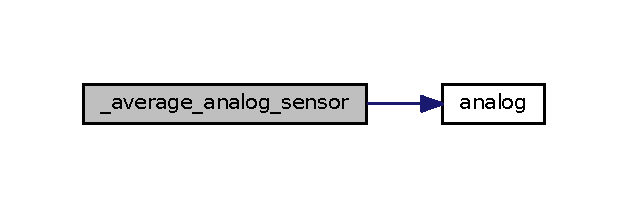
\includegraphics[width=302pt]{startstp_8c_aad36a7650fcfc97a17682202424cd242_cgraph}
\end{center}
\end{figure}




Here is the caller graph for this function\-:
\nopagebreak
\begin{figure}[H]
\begin{center}
\leavevmode
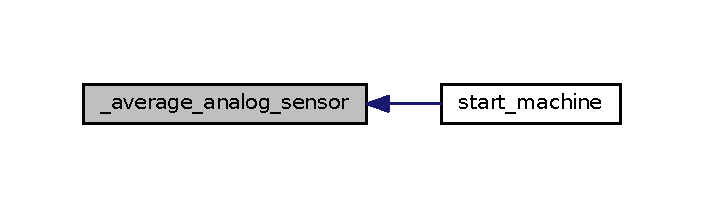
\includegraphics[width=338pt]{startstp_8c_aad36a7650fcfc97a17682202424cd242_icgraph}
\end{center}
\end{figure}


\hypertarget{startstp_8c_af49aa2ff6fdc9c54196bcec458bb3af4}{\index{startstp.\-c@{startstp.\-c}!\-\_\-stop\-\_\-machine@{\-\_\-stop\-\_\-machine}}
\index{\-\_\-stop\-\_\-machine@{\-\_\-stop\-\_\-machine}!startstp.c@{startstp.\-c}}
\subsubsection[{\-\_\-stop\-\_\-machine}]{\setlength{\rightskip}{0pt plus 5cm}void \-\_\-stop\-\_\-machine (
\begin{DoxyParamCaption}
\item[{float}]{time}
\end{DoxyParamCaption}
)}}\label{startstp_8c_af49aa2ff6fdc9c54196bcec458bb3af4}


Here is the call graph for this function\-:
\nopagebreak
\begin{figure}[H]
\begin{center}
\leavevmode
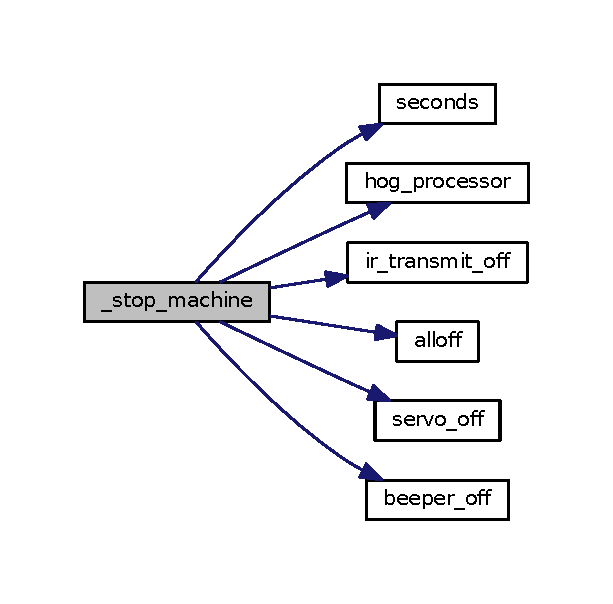
\includegraphics[width=294pt]{startstp_8c_af49aa2ff6fdc9c54196bcec458bb3af4_cgraph}
\end{center}
\end{figure}




Here is the caller graph for this function\-:
\nopagebreak
\begin{figure}[H]
\begin{center}
\leavevmode
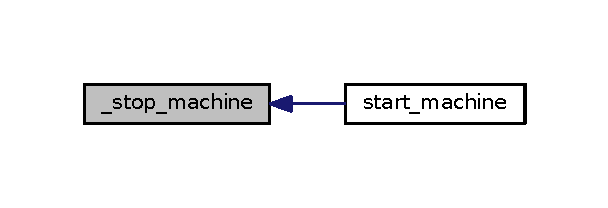
\includegraphics[width=292pt]{startstp_8c_af49aa2ff6fdc9c54196bcec458bb3af4_icgraph}
\end{center}
\end{figure}


\hypertarget{startstp_8c_ad098292050d6059ef0b3af84dac1ef6f}{\index{startstp.\-c@{startstp.\-c}!start\-\_\-machine@{start\-\_\-machine}}
\index{start\-\_\-machine@{start\-\_\-machine}!startstp.c@{startstp.\-c}}
\subsubsection[{start\-\_\-machine}]{\setlength{\rightskip}{0pt plus 5cm}void start\-\_\-machine (
\begin{DoxyParamCaption}
\item[{int}]{port}
\end{DoxyParamCaption}
)}}\label{startstp_8c_ad098292050d6059ef0b3af84dac1ef6f}


Here is the call graph for this function\-:
\nopagebreak
\begin{figure}[H]
\begin{center}
\leavevmode
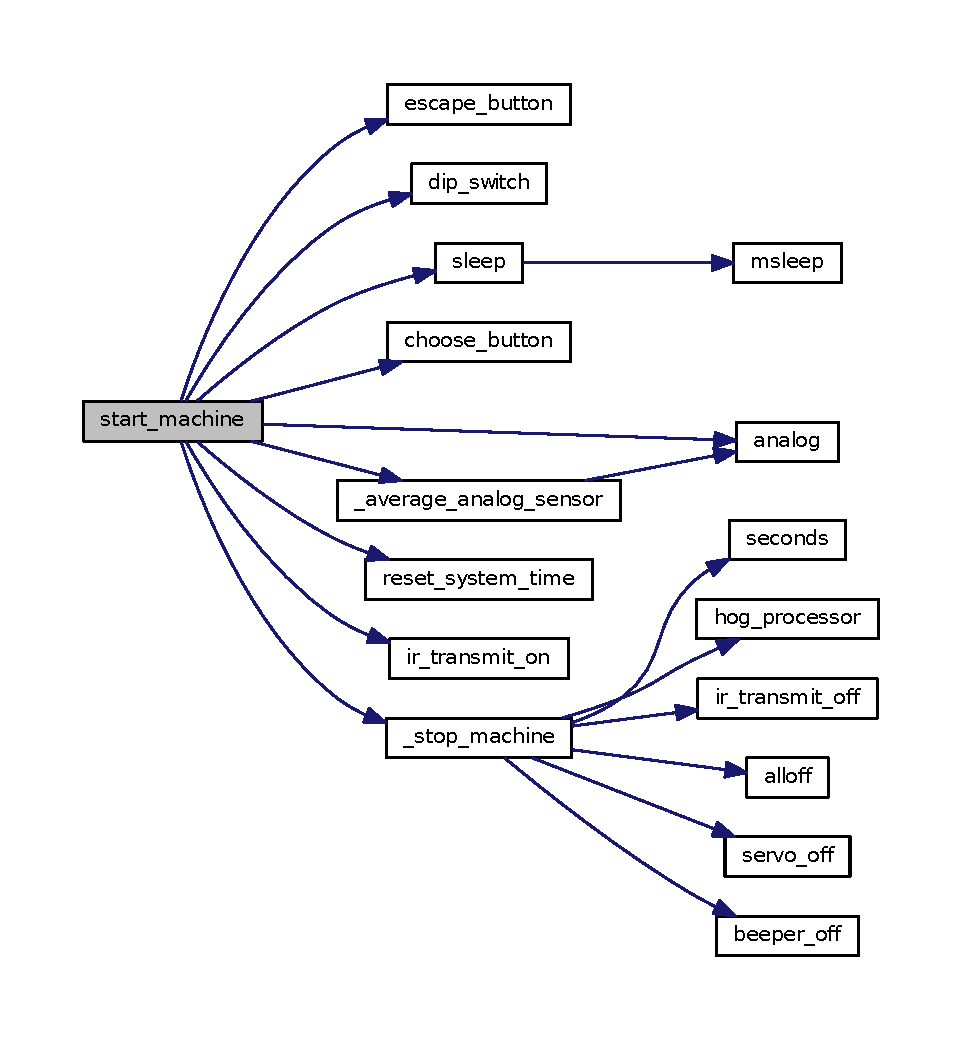
\includegraphics[width=350pt]{startstp_8c_ad098292050d6059ef0b3af84dac1ef6f_cgraph}
\end{center}
\end{figure}



\hypertarget{tunes_8c}{\section{/root/\-Desktop/rug-\/warrior/libs/base/tunes.c File Reference}
\label{tunes_8c}\index{/root/\-Desktop/rug-\/warrior/libs/base/tunes.\-c@{/root/\-Desktop/rug-\/warrior/libs/base/tunes.\-c}}
}
\subsection*{Functions}
\begin{DoxyCompactItemize}
\item 
void \hyperlink{tunes_8c_aab385898c7322dcbfda7e057e52f33d1}{pp} ()
\item 
void \hyperlink{tunes_8c_af6d9ec9e05c437b9572aa6bd07f93100}{wate} ()
\item 
void \hyperlink{tunes_8c_a991cece580a5054465383b47cadb0535}{classics} ()
\item 
void \hyperlink{tunes_8c_a31061818a5a2cf68539ca073374286d3}{charge} ()
\item 
void \hyperlink{tunes_8c_a32560516df494caa35d60ad505fb8086}{looney\-\_\-tune} ()
\item 
void \hyperlink{tunes_8c_a700ae836bbc833421cd1f7ac0f7460c4}{benny} ()
\item 
void \hyperlink{tunes_8c_acfec480eb7453765b7fa452e7b62f315}{musicbox} ()
\item 
void \hyperlink{tunes_8c_a61c7b7a1cc359cd0de25088e9c3d5017}{play} (char song\mbox{[}$\,$\mbox{]})
\item 
void \hyperlink{tunes_8c_a02f694a5858b7ab04b5f7d18c0f6be5e}{music\-\_\-command} (int \hyperlink{cof_8c_ae78103ab33f03590e84ff7bc735629d7}{c})
\item 
void \hyperlink{tunes_8c_a91cf8addb9d8e64913aa1aa559a65663}{play\-\_\-reset} ()
\item 
void \hyperlink{tunes_8c_a389a29b1aa7cd3e5f0ab7e0a50eb81c2}{play\-\_\-note} (int \hyperlink{cof_8c_a55c38cdc83b8334c8cb0a55638dfd650}{note}, int duration)
\item 
void \hyperlink{tunes_8c_ad64a752477bb35b9b4f09eec3f7e3281}{play\-\_\-note\-\_\-2} (int \hyperlink{cof_8c_a55c38cdc83b8334c8cb0a55638dfd650}{note}, int duration)
\item 
void \hyperlink{tunes_8c_a65053c134684581c6c673317b11ea735}{bicycle} ()
\end{DoxyCompactItemize}
\subsection*{Variables}
\begin{DoxyCompactItemize}
\item 
char \hyperlink{tunes_8c_a62b9882694b8c8c0e72c89d3fb824a10}{pp\-\_\-song} \mbox{[}$\,$\mbox{]} = \char`\"{}1\#d 4e3r1\#f4g3r1\#d 3e1\#f3g1c3b\-D1e3g1b 8\&b2b2a2g2e2d10e 7r1\#d 4e3r1\#f4g3r1\#d 3e1\#f3g1c3b1g3b1e 28\&e D3r1\#d 4e3r1\#f4g3r1\#d 3e1\#f3g1c3b\-D1e3g1b 8\&b2b2a2g2e2d10e 12r U3e1d3b1a3g1\#f 1\&b3a1\&b3a1\&b3a1\&b3a 2g2e2d2e18e 8r 2g2e2d2e18e 8r 2g2e2d2e18e\char`\"{}
\item 
char \hyperlink{tunes_8c_ab63ba636c250781677cfd4e980110c6b}{w\-\_\-song} \mbox{[}$\,$\mbox{]} = \char`\"{}1c2f1f2f1g2a1a2a1f2g1g2g1e4f1r 1f2a1a2a1\&b2c1c2c1c2d1c2\&b1a4g1r 1g\-U2d1d2d1c2d1e2f1d2c1d2c1\&b4a1r D1c2f1f2f1g2a1a2a1f2g1g2f1e5f\char`\"{}
\item 
char \hyperlink{tunes_8c_a6708a4c9ea868f6db08e201b14061acc}{classics\-\_\-song} \mbox{[}$\,$\mbox{]} = \char`\"{}4g2c2d4c4g4a2g2f2e2c2d2e2f2g2a2b10c2r 4c4b4c2d2b2c2d2e2\#f4g2\#f2e4d2g2\#f4g4d4e2d2c2b2g2a2b2c2b2c2d2e2d2e2\#f12g\char`\"{}
\item 
char \hyperlink{tunes_8c_a15a97d11c4678bb389088c1899ad7ed6}{charge\-\_\-song} \mbox{[}$\,$\mbox{]} = \char`\"{}1c1e1g2c1r1g4c\char`\"{}
\item 
char \hyperlink{tunes_8c_a09d38809cea08dc8772e0dd76c88d066}{benny\-\_\-song} \mbox{[}$\,$\mbox{]} = \char`\"{}1c1d1c\-U2f2f1d1c1\#g1a2c2d1c1a1\#g1g2f1f1f1a1c2d5c1c1d1c2f2f1d1c1\#g1a2c2d1c1a1\#g1g2c1c1c1e1g2e5c1c1d1c2f2f2f2f2f2f1d1c1g1a2\#a2\#a2\#a2\#a1d1\#a1d1\#a\-U1f3g1a1\#g1a1\#g1a3c1a1\#g1\#a5f1a1\#f1\#d1c\-U1\#g1f1d1b4f\char`\"{}
\item 
char \hyperlink{tunes_8c_a7317d27468a5ce138ebc153fdc108c9e}{mb\-\_\-song1} \mbox{[}$\,$\mbox{]} = \char`\"{}2c2e2g2e\-U2c2g2e2g\-D2c2e2g2e\-U2c2g2e 2c2c2g2c2e2c2e2g\-D2c\-U2c2b2a7g1r 2g2g2f2d2b2g2b2d2f2e2c\-U2a7g1r D2c2c2g2c2e2c2e2g\-D2c\-U2c2b2a7g1r 2g2g2f2d2b2g2b2d2b2c2g\-U2e4c 2c2e2g2c2a2f2c2a2c2f2a2g\-D2c\-U2a4g D2g2b2d2g2f2d2b2g2b2d2f2e2c\-U2a4g D2c2e2g2c2a2f2c2a2c2f2a2g\-D2c\-U2a4g D2g2b2d2g2f2d2b2g2b2d2b2c2g\-U2e7c\char`\"{}
\item 
char \hyperlink{tunes_8c_afded93bc1107bacc40b7979589eda5fe}{mb\-\_\-song2} \mbox{[}$\,$\mbox{]} = \char`\"{}2c2e2g2e\-U2c2g2e2g\-D2c2e2g2e\-U2c2g2e 2c2c2g2c2e2c2e2g\-D2c\-U2c2b2a7g1r U2g2g2f2d2b2g2b2d2f2e2c\-U2a7g1r D\-D2c2c2g2c2e2c2e2g\-D2c\-U2c2b2a7g1r U2g2g2f2d2b2g2b2d2b2c2g\-U2e4c 2c2e2g2c2a2f2c2a2c2f2a2g\-D2c\-U2a4g D2g2b2d2g2f2d2b2g2b2d2f2e2c\-U2a4g D\-D2c2e2g2c2a2f2c2a2c2f2a2g\-D2c\-U2a4g U2g2b2d2g2f2d2b2g2b2d2b2c2g\-U2e7c\char`\"{}
\item 
char \hyperlink{tunes_8c_aee268afad37d51980e98ead7c22eb4fa}{looney\-\_\-tune\-\_\-song} \mbox{[}$\,$\mbox{]} = \char`\"{}U3e1d2c2d2e2d2e2c2d2d2d6d2r 3d1c2b2c2d2\#c2d2b2c2c2c6c\char`\"{}
\item 
int \hyperlink{tunes_8c_a516115750e956e7c851392eeb95d7dcb}{tempo} = 12
\item 
long \hyperlink{tunes_8c_a8667588dec524bf854d0c16771d425a1}{time}
\item 
long \hyperlink{tunes_8c_a14a78a37b71652800b63a938f3bdbcd6}{newtime}
\item 
int \hyperlink{tunes_8c_aadc4454f2dccae1e14303fa33c486a39}{music\-\_\-current\-\_\-command} = 'o'
\item 
int \hyperlink{tunes_8c_a586e7a3d7ad578641663ee805f3d813b}{music\-\_\-next\-\_\-command} = 0
\end{DoxyCompactItemize}


\subsection{Function Documentation}
\hypertarget{tunes_8c_a700ae836bbc833421cd1f7ac0f7460c4}{\index{tunes.\-c@{tunes.\-c}!benny@{benny}}
\index{benny@{benny}!tunes.c@{tunes.\-c}}
\subsubsection[{benny}]{\setlength{\rightskip}{0pt plus 5cm}void benny (
\begin{DoxyParamCaption}
{}
\end{DoxyParamCaption}
)}}\label{tunes_8c_a700ae836bbc833421cd1f7ac0f7460c4}


Here is the call graph for this function\-:
\nopagebreak
\begin{figure}[H]
\begin{center}
\leavevmode
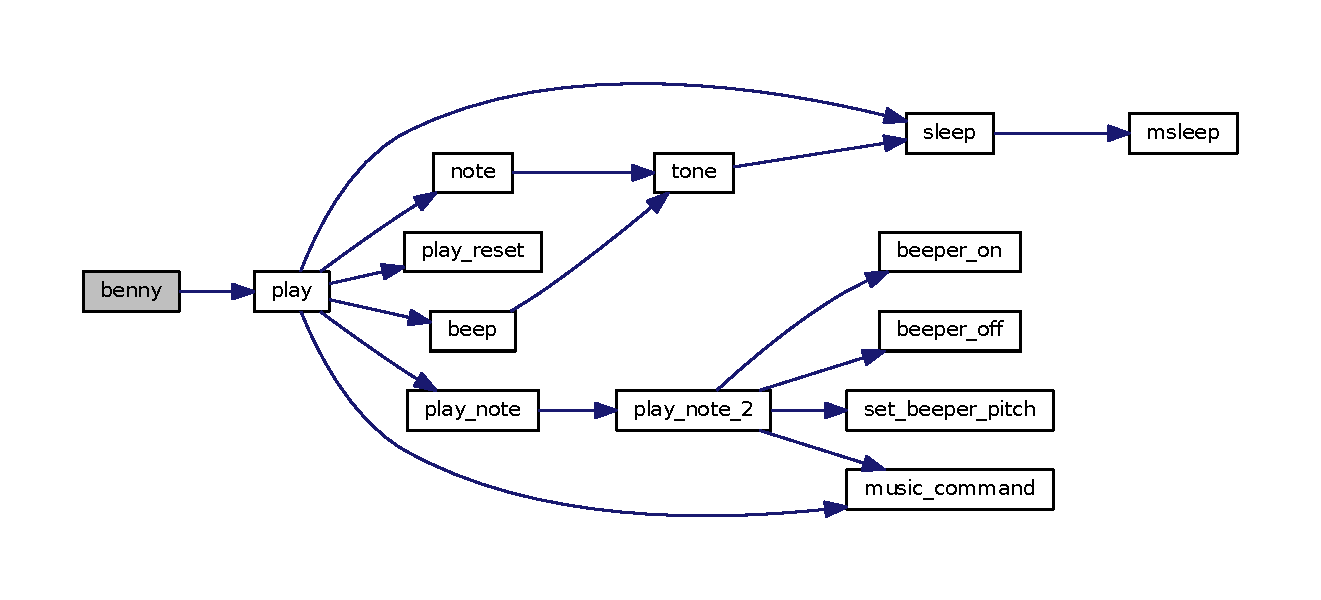
\includegraphics[width=350pt]{tunes_8c_a700ae836bbc833421cd1f7ac0f7460c4_cgraph}
\end{center}
\end{figure}


\hypertarget{tunes_8c_a65053c134684581c6c673317b11ea735}{\index{tunes.\-c@{tunes.\-c}!bicycle@{bicycle}}
\index{bicycle@{bicycle}!tunes.c@{tunes.\-c}}
\subsubsection[{bicycle}]{\setlength{\rightskip}{0pt plus 5cm}void bicycle (
\begin{DoxyParamCaption}
{}
\end{DoxyParamCaption}
)}}\label{tunes_8c_a65053c134684581c6c673317b11ea735}


Here is the call graph for this function\-:
\nopagebreak
\begin{figure}[H]
\begin{center}
\leavevmode
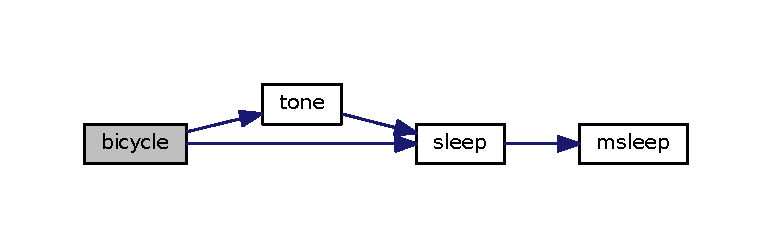
\includegraphics[width=350pt]{tunes_8c_a65053c134684581c6c673317b11ea735_cgraph}
\end{center}
\end{figure}


\hypertarget{tunes_8c_a31061818a5a2cf68539ca073374286d3}{\index{tunes.\-c@{tunes.\-c}!charge@{charge}}
\index{charge@{charge}!tunes.c@{tunes.\-c}}
\subsubsection[{charge}]{\setlength{\rightskip}{0pt plus 5cm}void charge (
\begin{DoxyParamCaption}
{}
\end{DoxyParamCaption}
)}}\label{tunes_8c_a31061818a5a2cf68539ca073374286d3}


Here is the call graph for this function\-:
\nopagebreak
\begin{figure}[H]
\begin{center}
\leavevmode
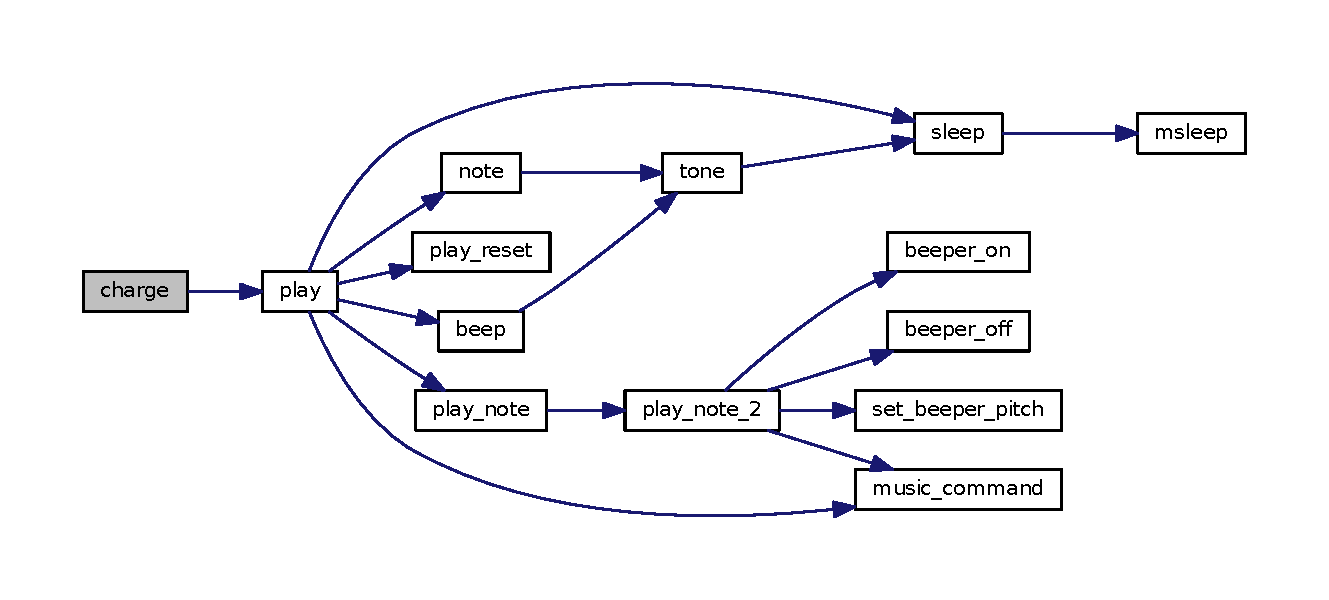
\includegraphics[width=350pt]{tunes_8c_a31061818a5a2cf68539ca073374286d3_cgraph}
\end{center}
\end{figure}


\hypertarget{tunes_8c_a991cece580a5054465383b47cadb0535}{\index{tunes.\-c@{tunes.\-c}!classics@{classics}}
\index{classics@{classics}!tunes.c@{tunes.\-c}}
\subsubsection[{classics}]{\setlength{\rightskip}{0pt plus 5cm}void classics (
\begin{DoxyParamCaption}
{}
\end{DoxyParamCaption}
)}}\label{tunes_8c_a991cece580a5054465383b47cadb0535}


Here is the call graph for this function\-:
\nopagebreak
\begin{figure}[H]
\begin{center}
\leavevmode
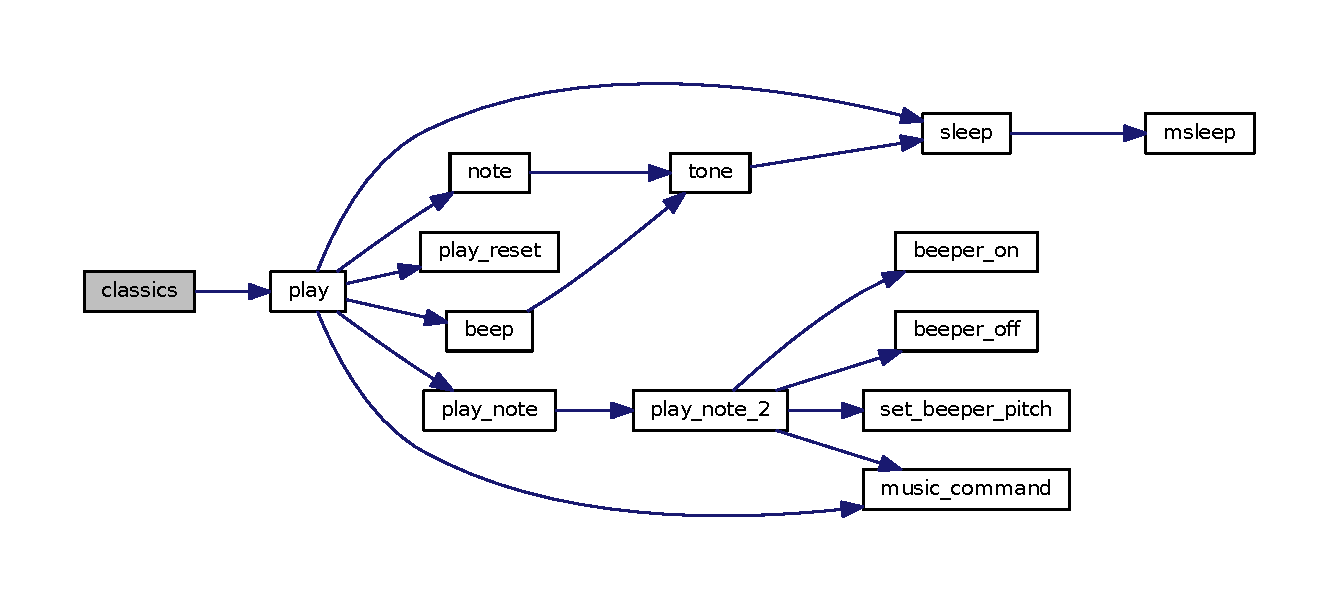
\includegraphics[width=350pt]{tunes_8c_a991cece580a5054465383b47cadb0535_cgraph}
\end{center}
\end{figure}


\hypertarget{tunes_8c_a32560516df494caa35d60ad505fb8086}{\index{tunes.\-c@{tunes.\-c}!looney\-\_\-tune@{looney\-\_\-tune}}
\index{looney\-\_\-tune@{looney\-\_\-tune}!tunes.c@{tunes.\-c}}
\subsubsection[{looney\-\_\-tune}]{\setlength{\rightskip}{0pt plus 5cm}void looney\-\_\-tune (
\begin{DoxyParamCaption}
{}
\end{DoxyParamCaption}
)}}\label{tunes_8c_a32560516df494caa35d60ad505fb8086}


Here is the call graph for this function\-:
\nopagebreak
\begin{figure}[H]
\begin{center}
\leavevmode
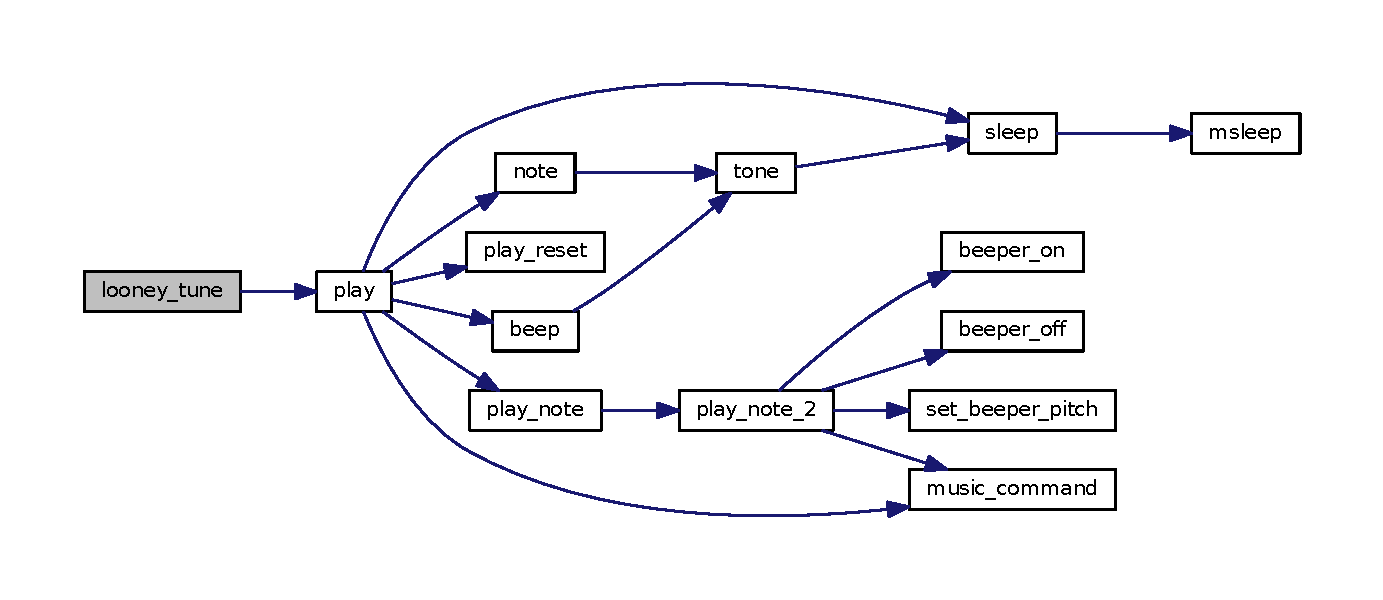
\includegraphics[width=350pt]{tunes_8c_a32560516df494caa35d60ad505fb8086_cgraph}
\end{center}
\end{figure}


\hypertarget{tunes_8c_a02f694a5858b7ab04b5f7d18c0f6be5e}{\index{tunes.\-c@{tunes.\-c}!music\-\_\-command@{music\-\_\-command}}
\index{music\-\_\-command@{music\-\_\-command}!tunes.c@{tunes.\-c}}
\subsubsection[{music\-\_\-command}]{\setlength{\rightskip}{0pt plus 5cm}void music\-\_\-command (
\begin{DoxyParamCaption}
\item[{int}]{c}
\end{DoxyParamCaption}
)}}\label{tunes_8c_a02f694a5858b7ab04b5f7d18c0f6be5e}


Here is the caller graph for this function\-:
\nopagebreak
\begin{figure}[H]
\begin{center}
\leavevmode
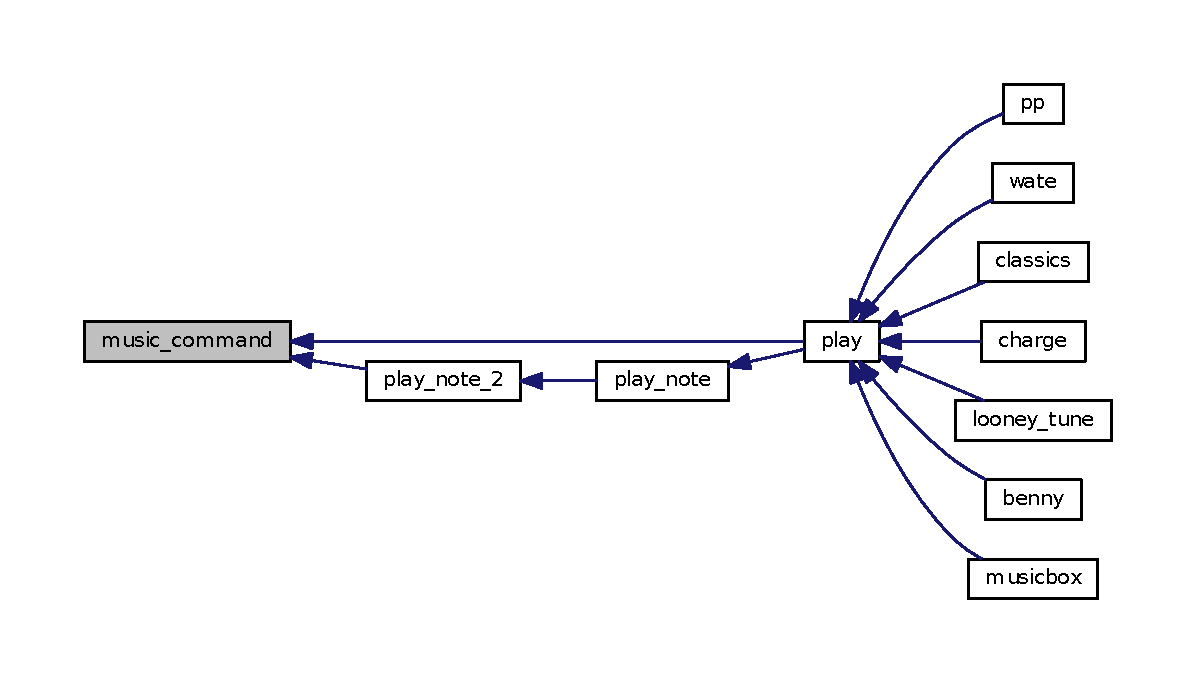
\includegraphics[width=350pt]{tunes_8c_a02f694a5858b7ab04b5f7d18c0f6be5e_icgraph}
\end{center}
\end{figure}


\hypertarget{tunes_8c_acfec480eb7453765b7fa452e7b62f315}{\index{tunes.\-c@{tunes.\-c}!musicbox@{musicbox}}
\index{musicbox@{musicbox}!tunes.c@{tunes.\-c}}
\subsubsection[{musicbox}]{\setlength{\rightskip}{0pt plus 5cm}void musicbox (
\begin{DoxyParamCaption}
{}
\end{DoxyParamCaption}
)}}\label{tunes_8c_acfec480eb7453765b7fa452e7b62f315}


Here is the call graph for this function\-:
\nopagebreak
\begin{figure}[H]
\begin{center}
\leavevmode
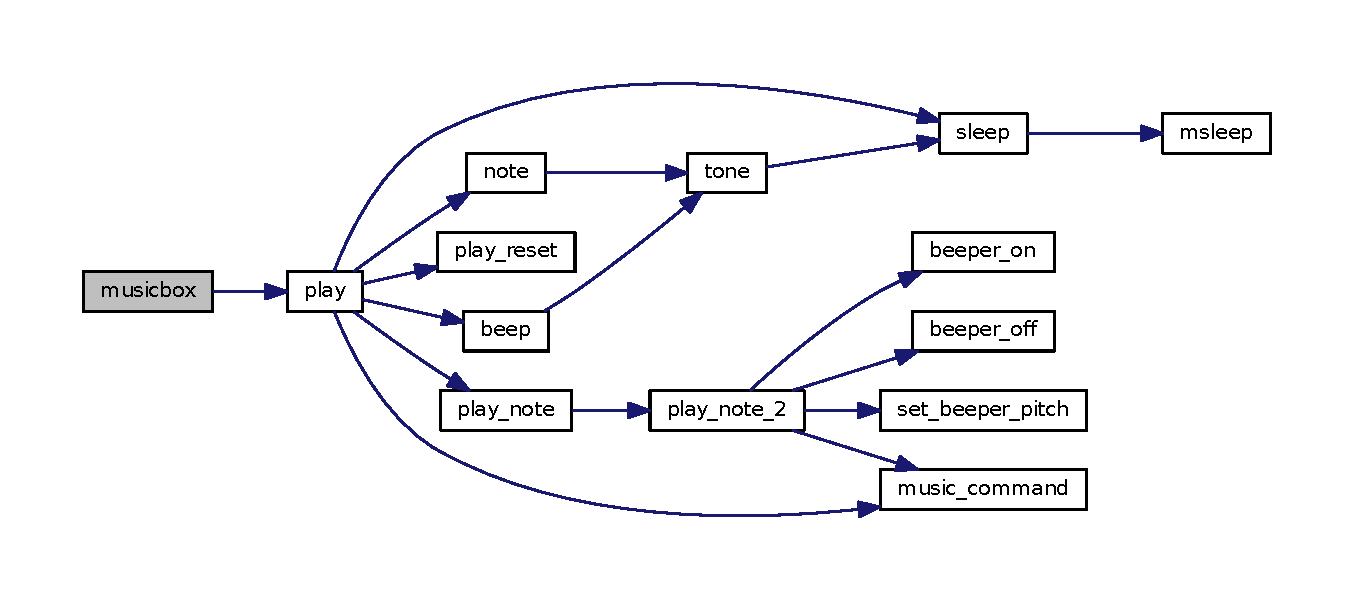
\includegraphics[width=350pt]{tunes_8c_acfec480eb7453765b7fa452e7b62f315_cgraph}
\end{center}
\end{figure}


\hypertarget{tunes_8c_a61c7b7a1cc359cd0de25088e9c3d5017}{\index{tunes.\-c@{tunes.\-c}!play@{play}}
\index{play@{play}!tunes.c@{tunes.\-c}}
\subsubsection[{play}]{\setlength{\rightskip}{0pt plus 5cm}void play (
\begin{DoxyParamCaption}
\item[{char}]{song\mbox{[}$\,$\mbox{]}}
\end{DoxyParamCaption}
)}}\label{tunes_8c_a61c7b7a1cc359cd0de25088e9c3d5017}


Here is the call graph for this function\-:
\nopagebreak
\begin{figure}[H]
\begin{center}
\leavevmode
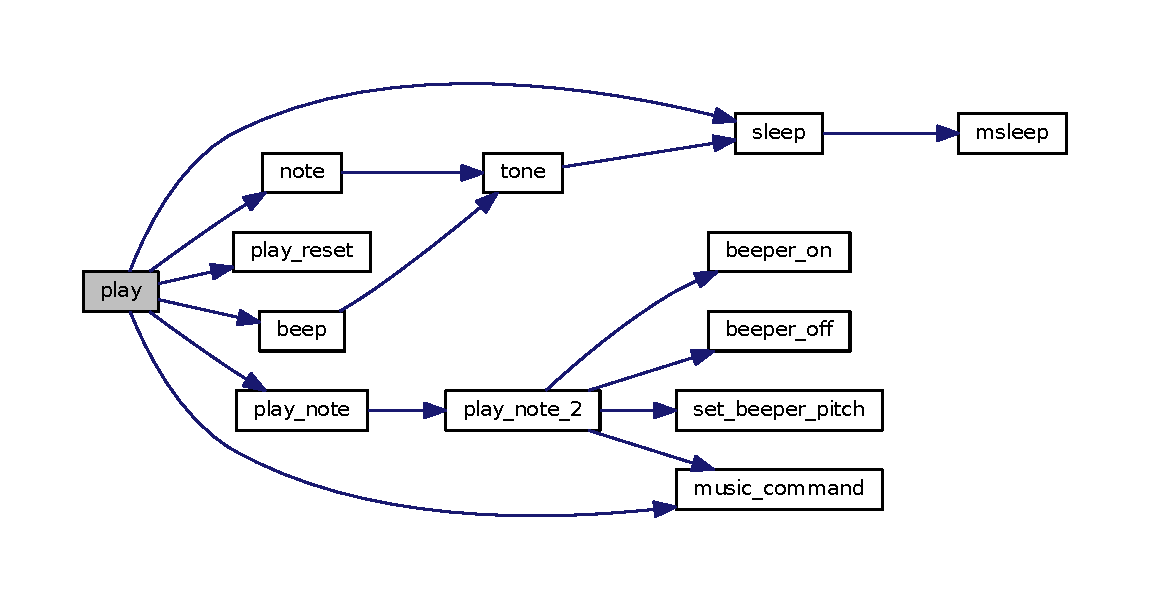
\includegraphics[width=350pt]{tunes_8c_a61c7b7a1cc359cd0de25088e9c3d5017_cgraph}
\end{center}
\end{figure}




Here is the caller graph for this function\-:
\nopagebreak
\begin{figure}[H]
\begin{center}
\leavevmode
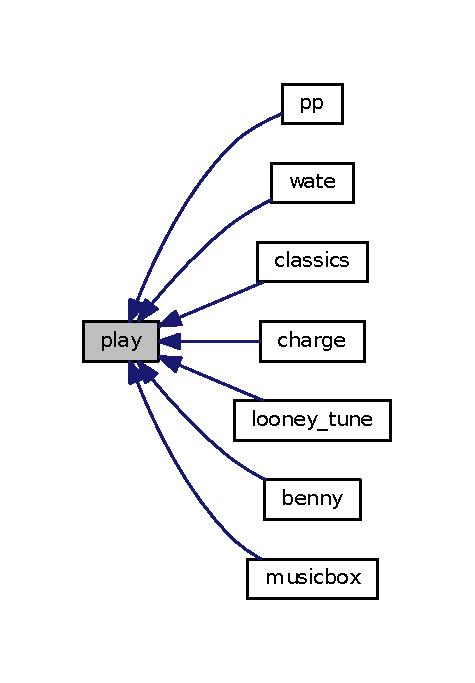
\includegraphics[width=228pt]{tunes_8c_a61c7b7a1cc359cd0de25088e9c3d5017_icgraph}
\end{center}
\end{figure}


\hypertarget{tunes_8c_a389a29b1aa7cd3e5f0ab7e0a50eb81c2}{\index{tunes.\-c@{tunes.\-c}!play\-\_\-note@{play\-\_\-note}}
\index{play\-\_\-note@{play\-\_\-note}!tunes.c@{tunes.\-c}}
\subsubsection[{play\-\_\-note}]{\setlength{\rightskip}{0pt plus 5cm}void play\-\_\-note (
\begin{DoxyParamCaption}
\item[{int}]{note, }
\item[{int}]{duration}
\end{DoxyParamCaption}
)}}\label{tunes_8c_a389a29b1aa7cd3e5f0ab7e0a50eb81c2}


Here is the call graph for this function\-:
\nopagebreak
\begin{figure}[H]
\begin{center}
\leavevmode
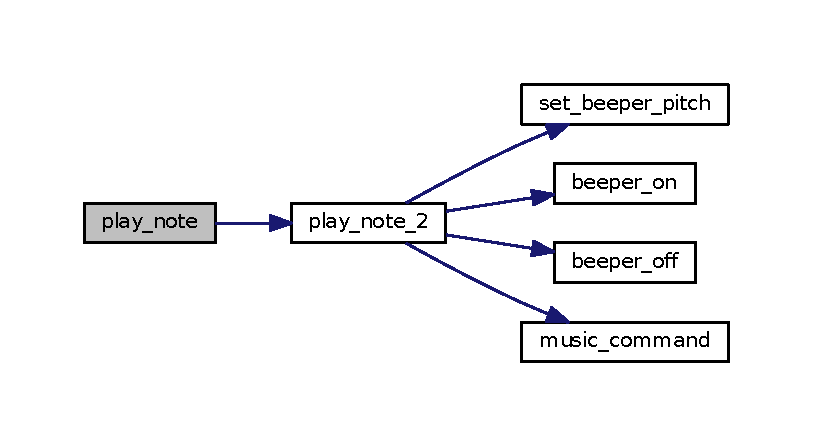
\includegraphics[width=350pt]{tunes_8c_a389a29b1aa7cd3e5f0ab7e0a50eb81c2_cgraph}
\end{center}
\end{figure}




Here is the caller graph for this function\-:
\nopagebreak
\begin{figure}[H]
\begin{center}
\leavevmode
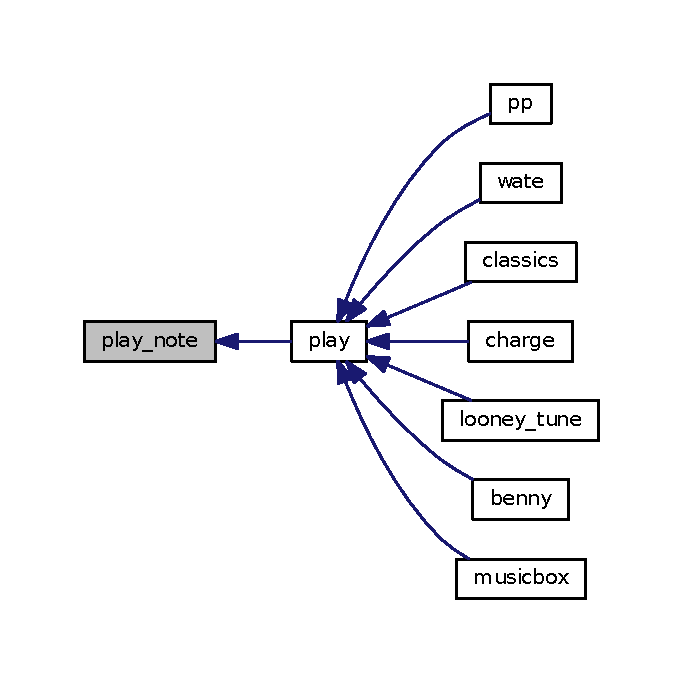
\includegraphics[width=328pt]{tunes_8c_a389a29b1aa7cd3e5f0ab7e0a50eb81c2_icgraph}
\end{center}
\end{figure}


\hypertarget{tunes_8c_ad64a752477bb35b9b4f09eec3f7e3281}{\index{tunes.\-c@{tunes.\-c}!play\-\_\-note\-\_\-2@{play\-\_\-note\-\_\-2}}
\index{play\-\_\-note\-\_\-2@{play\-\_\-note\-\_\-2}!tunes.c@{tunes.\-c}}
\subsubsection[{play\-\_\-note\-\_\-2}]{\setlength{\rightskip}{0pt plus 5cm}void play\-\_\-note\-\_\-2 (
\begin{DoxyParamCaption}
\item[{int}]{note, }
\item[{int}]{duration}
\end{DoxyParamCaption}
)}}\label{tunes_8c_ad64a752477bb35b9b4f09eec3f7e3281}


Here is the call graph for this function\-:
\nopagebreak
\begin{figure}[H]
\begin{center}
\leavevmode
\includegraphics[width=290pt]{tunes_8c_ad64a752477bb35b9b4f09eec3f7e3281_cgraph}
\end{center}
\end{figure}




Here is the caller graph for this function\-:
\nopagebreak
\begin{figure}[H]
\begin{center}
\leavevmode
\includegraphics[width=350pt]{tunes_8c_ad64a752477bb35b9b4f09eec3f7e3281_icgraph}
\end{center}
\end{figure}


\hypertarget{tunes_8c_a91cf8addb9d8e64913aa1aa559a65663}{\index{tunes.\-c@{tunes.\-c}!play\-\_\-reset@{play\-\_\-reset}}
\index{play\-\_\-reset@{play\-\_\-reset}!tunes.c@{tunes.\-c}}
\subsubsection[{play\-\_\-reset}]{\setlength{\rightskip}{0pt plus 5cm}void play\-\_\-reset (
\begin{DoxyParamCaption}
{}
\end{DoxyParamCaption}
)}}\label{tunes_8c_a91cf8addb9d8e64913aa1aa559a65663}


Here is the caller graph for this function\-:
\nopagebreak
\begin{figure}[H]
\begin{center}
\leavevmode
\includegraphics[width=330pt]{tunes_8c_a91cf8addb9d8e64913aa1aa559a65663_icgraph}
\end{center}
\end{figure}


\hypertarget{tunes_8c_aab385898c7322dcbfda7e057e52f33d1}{\index{tunes.\-c@{tunes.\-c}!pp@{pp}}
\index{pp@{pp}!tunes.c@{tunes.\-c}}
\subsubsection[{pp}]{\setlength{\rightskip}{0pt plus 5cm}void pp (
\begin{DoxyParamCaption}
{}
\end{DoxyParamCaption}
)}}\label{tunes_8c_aab385898c7322dcbfda7e057e52f33d1}


Here is the call graph for this function\-:
\nopagebreak
\begin{figure}[H]
\begin{center}
\leavevmode
\includegraphics[width=350pt]{tunes_8c_aab385898c7322dcbfda7e057e52f33d1_cgraph}
\end{center}
\end{figure}


\hypertarget{tunes_8c_af6d9ec9e05c437b9572aa6bd07f93100}{\index{tunes.\-c@{tunes.\-c}!wate@{wate}}
\index{wate@{wate}!tunes.c@{tunes.\-c}}
\subsubsection[{wate}]{\setlength{\rightskip}{0pt plus 5cm}void wate (
\begin{DoxyParamCaption}
{}
\end{DoxyParamCaption}
)}}\label{tunes_8c_af6d9ec9e05c437b9572aa6bd07f93100}


Here is the call graph for this function\-:
\nopagebreak
\begin{figure}[H]
\begin{center}
\leavevmode
\includegraphics[width=350pt]{tunes_8c_af6d9ec9e05c437b9572aa6bd07f93100_cgraph}
\end{center}
\end{figure}




\subsection{Variable Documentation}
\hypertarget{tunes_8c_a09d38809cea08dc8772e0dd76c88d066}{\index{tunes.\-c@{tunes.\-c}!benny\-\_\-song@{benny\-\_\-song}}
\index{benny\-\_\-song@{benny\-\_\-song}!tunes.c@{tunes.\-c}}
\subsubsection[{benny\-\_\-song}]{\setlength{\rightskip}{0pt plus 5cm}char benny\-\_\-song\mbox{[}$\,$\mbox{]} = \char`\"{}1c1d1c\-U2f2f1d1c1\#g1a2c2d1c1a1\#g1g2f1f1f1a1c2d5c1c1d1c2f2f1d1c1\#g1a2c2d1c1a1\#g1g2c1c1c1e1g2e5c1c1d1c2f2f2f2f2f2f1d1c1g1a2\#a2\#a2\#a2\#a1d1\#a1d1\#a\-U1f3g1a1\#g1a1\#g1a3c1a1\#g1\#a5f1a1\#f1\#d1c\-U1\#g1f1d1b4f\char`\"{}}}\label{tunes_8c_a09d38809cea08dc8772e0dd76c88d066}
\hypertarget{tunes_8c_a15a97d11c4678bb389088c1899ad7ed6}{\index{tunes.\-c@{tunes.\-c}!charge\-\_\-song@{charge\-\_\-song}}
\index{charge\-\_\-song@{charge\-\_\-song}!tunes.c@{tunes.\-c}}
\subsubsection[{charge\-\_\-song}]{\setlength{\rightskip}{0pt plus 5cm}char charge\-\_\-song\mbox{[}$\,$\mbox{]} = \char`\"{}1c1e1g2c1r1g4c\char`\"{}}}\label{tunes_8c_a15a97d11c4678bb389088c1899ad7ed6}
\hypertarget{tunes_8c_a6708a4c9ea868f6db08e201b14061acc}{\index{tunes.\-c@{tunes.\-c}!classics\-\_\-song@{classics\-\_\-song}}
\index{classics\-\_\-song@{classics\-\_\-song}!tunes.c@{tunes.\-c}}
\subsubsection[{classics\-\_\-song}]{\setlength{\rightskip}{0pt plus 5cm}char classics\-\_\-song\mbox{[}$\,$\mbox{]} = \char`\"{}4g2c2d4c4g4a2g2f2e2c2d2e2f2g2a2b10c2r 4c4b4c2d2b2c2d2e2\#f4g2\#f2e4d2g2\#f4g4d4e2d2c2b2g2a2b2c2b2c2d2e2d2e2\#f12g\char`\"{}}}\label{tunes_8c_a6708a4c9ea868f6db08e201b14061acc}
\hypertarget{tunes_8c_aee268afad37d51980e98ead7c22eb4fa}{\index{tunes.\-c@{tunes.\-c}!looney\-\_\-tune\-\_\-song@{looney\-\_\-tune\-\_\-song}}
\index{looney\-\_\-tune\-\_\-song@{looney\-\_\-tune\-\_\-song}!tunes.c@{tunes.\-c}}
\subsubsection[{looney\-\_\-tune\-\_\-song}]{\setlength{\rightskip}{0pt plus 5cm}char looney\-\_\-tune\-\_\-song\mbox{[}$\,$\mbox{]} = \char`\"{}U3e1d2c2d2e2d2e2c2d2d2d6d2r 3d1c2b2c2d2\#c2d2b2c2c2c6c\char`\"{}}}\label{tunes_8c_aee268afad37d51980e98ead7c22eb4fa}
\hypertarget{tunes_8c_a7317d27468a5ce138ebc153fdc108c9e}{\index{tunes.\-c@{tunes.\-c}!mb\-\_\-song1@{mb\-\_\-song1}}
\index{mb\-\_\-song1@{mb\-\_\-song1}!tunes.c@{tunes.\-c}}
\subsubsection[{mb\-\_\-song1}]{\setlength{\rightskip}{0pt plus 5cm}char mb\-\_\-song1\mbox{[}$\,$\mbox{]} = \char`\"{}2c2e2g2e\-U2c2g2e2g\-D2c2e2g2e\-U2c2g2e 2c2c2g2c2e2c2e2g\-D2c\-U2c2b2a7g1r 2g2g2f2d2b2g2b2d2f2e2c\-U2a7g1r D2c2c2g2c2e2c2e2g\-D2c\-U2c2b2a7g1r 2g2g2f2d2b2g2b2d2b2c2g\-U2e4c 2c2e2g2c2a2f2c2a2c2f2a2g\-D2c\-U2a4g D2g2b2d2g2f2d2b2g2b2d2f2e2c\-U2a4g D2c2e2g2c2a2f2c2a2c2f2a2g\-D2c\-U2a4g D2g2b2d2g2f2d2b2g2b2d2b2c2g\-U2e7c\char`\"{}}}\label{tunes_8c_a7317d27468a5ce138ebc153fdc108c9e}
\hypertarget{tunes_8c_afded93bc1107bacc40b7979589eda5fe}{\index{tunes.\-c@{tunes.\-c}!mb\-\_\-song2@{mb\-\_\-song2}}
\index{mb\-\_\-song2@{mb\-\_\-song2}!tunes.c@{tunes.\-c}}
\subsubsection[{mb\-\_\-song2}]{\setlength{\rightskip}{0pt plus 5cm}char mb\-\_\-song2\mbox{[}$\,$\mbox{]} = \char`\"{}2c2e2g2e\-U2c2g2e2g\-D2c2e2g2e\-U2c2g2e 2c2c2g2c2e2c2e2g\-D2c\-U2c2b2a7g1r U2g2g2f2d2b2g2b2d2f2e2c\-U2a7g1r D\-D2c2c2g2c2e2c2e2g\-D2c\-U2c2b2a7g1r U2g2g2f2d2b2g2b2d2b2c2g\-U2e4c 2c2e2g2c2a2f2c2a2c2f2a2g\-D2c\-U2a4g D2g2b2d2g2f2d2b2g2b2d2f2e2c\-U2a4g D\-D2c2e2g2c2a2f2c2a2c2f2a2g\-D2c\-U2a4g U2g2b2d2g2f2d2b2g2b2d2b2c2g\-U2e7c\char`\"{}}}\label{tunes_8c_afded93bc1107bacc40b7979589eda5fe}
\hypertarget{tunes_8c_aadc4454f2dccae1e14303fa33c486a39}{\index{tunes.\-c@{tunes.\-c}!music\-\_\-current\-\_\-command@{music\-\_\-current\-\_\-command}}
\index{music\-\_\-current\-\_\-command@{music\-\_\-current\-\_\-command}!tunes.c@{tunes.\-c}}
\subsubsection[{music\-\_\-current\-\_\-command}]{\setlength{\rightskip}{0pt plus 5cm}int music\-\_\-current\-\_\-command = 'o'}}\label{tunes_8c_aadc4454f2dccae1e14303fa33c486a39}
\hypertarget{tunes_8c_a586e7a3d7ad578641663ee805f3d813b}{\index{tunes.\-c@{tunes.\-c}!music\-\_\-next\-\_\-command@{music\-\_\-next\-\_\-command}}
\index{music\-\_\-next\-\_\-command@{music\-\_\-next\-\_\-command}!tunes.c@{tunes.\-c}}
\subsubsection[{music\-\_\-next\-\_\-command}]{\setlength{\rightskip}{0pt plus 5cm}int music\-\_\-next\-\_\-command = 0}}\label{tunes_8c_a586e7a3d7ad578641663ee805f3d813b}
\hypertarget{tunes_8c_a14a78a37b71652800b63a938f3bdbcd6}{\index{tunes.\-c@{tunes.\-c}!newtime@{newtime}}
\index{newtime@{newtime}!tunes.c@{tunes.\-c}}
\subsubsection[{newtime}]{\setlength{\rightskip}{0pt plus 5cm}long newtime}}\label{tunes_8c_a14a78a37b71652800b63a938f3bdbcd6}
\hypertarget{tunes_8c_a62b9882694b8c8c0e72c89d3fb824a10}{\index{tunes.\-c@{tunes.\-c}!pp\-\_\-song@{pp\-\_\-song}}
\index{pp\-\_\-song@{pp\-\_\-song}!tunes.c@{tunes.\-c}}
\subsubsection[{pp\-\_\-song}]{\setlength{\rightskip}{0pt plus 5cm}char pp\-\_\-song\mbox{[}$\,$\mbox{]} = \char`\"{}1\#d 4e3r1\#f4g3r1\#d 3e1\#f3g1c3b\-D1e3g1b 8\&b2b2a2g2e2d10e 7r1\#d 4e3r1\#f4g3r1\#d 3e1\#f3g1c3b1g3b1e 28\&e D3r1\#d 4e3r1\#f4g3r1\#d 3e1\#f3g1c3b\-D1e3g1b 8\&b2b2a2g2e2d10e 12r U3e1d3b1a3g1\#f 1\&b3a1\&b3a1\&b3a1\&b3a 2g2e2d2e18e 8r 2g2e2d2e18e 8r 2g2e2d2e18e\char`\"{}}}\label{tunes_8c_a62b9882694b8c8c0e72c89d3fb824a10}
\hypertarget{tunes_8c_a516115750e956e7c851392eeb95d7dcb}{\index{tunes.\-c@{tunes.\-c}!tempo@{tempo}}
\index{tempo@{tempo}!tunes.c@{tunes.\-c}}
\subsubsection[{tempo}]{\setlength{\rightskip}{0pt plus 5cm}int tempo = 12}}\label{tunes_8c_a516115750e956e7c851392eeb95d7dcb}
\hypertarget{tunes_8c_a8667588dec524bf854d0c16771d425a1}{\index{tunes.\-c@{tunes.\-c}!time@{time}}
\index{time@{time}!tunes.c@{tunes.\-c}}
\subsubsection[{time}]{\setlength{\rightskip}{0pt plus 5cm}long time}}\label{tunes_8c_a8667588dec524bf854d0c16771d425a1}
\hypertarget{tunes_8c_ab63ba636c250781677cfd4e980110c6b}{\index{tunes.\-c@{tunes.\-c}!w\-\_\-song@{w\-\_\-song}}
\index{w\-\_\-song@{w\-\_\-song}!tunes.c@{tunes.\-c}}
\subsubsection[{w\-\_\-song}]{\setlength{\rightskip}{0pt plus 5cm}char w\-\_\-song\mbox{[}$\,$\mbox{]} = \char`\"{}1c2f1f2f1g2a1a2a1f2g1g2g1e4f1r 1f2a1a2a1\&b2c1c2c1c2d1c2\&b1a4g1r 1g\-U2d1d2d1c2d1e2f1d2c1d2c1\&b4a1r D1c2f1f2f1g2a1a2a1f2g1g2f1e5f\char`\"{}}}\label{tunes_8c_ab63ba636c250781677cfd4e980110c6b}

\hypertarget{1meter_8c}{\section{/root/\-Desktop/rug-\/warrior/libs/behavior/1meter.c File Reference}
\label{1meter_8c}\index{/root/\-Desktop/rug-\/warrior/libs/behavior/1meter.\-c@{/root/\-Desktop/rug-\/warrior/libs/behavior/1meter.\-c}}
}
\subsection*{Functions}
\begin{DoxyCompactItemize}
\item 
void \hyperlink{1meter_8c_acdef7a1fd863a6d3770c1268cb06add3}{main} ()
\end{DoxyCompactItemize}


\subsection{Function Documentation}
\hypertarget{1meter_8c_acdef7a1fd863a6d3770c1268cb06add3}{\index{1meter.\-c@{1meter.\-c}!main@{main}}
\index{main@{main}!1meter.c@{1meter.\-c}}
\subsubsection[{main}]{\setlength{\rightskip}{0pt plus 5cm}void main (
\begin{DoxyParamCaption}
{}
\end{DoxyParamCaption}
)}}\label{1meter_8c_acdef7a1fd863a6d3770c1268cb06add3}


Here is the call graph for this function\-:
\nopagebreak
\begin{figure}[H]
\begin{center}
\leavevmode
\includegraphics[width=320pt]{1meter_8c_acdef7a1fd863a6d3770c1268cb06add3_cgraph}
\end{center}
\end{figure}



\hypertarget{rotate_8c}{\section{/root/\-Desktop/rug-\/warrior/libs/behavior/rotate.c File Reference}
\label{rotate_8c}\index{/root/\-Desktop/rug-\/warrior/libs/behavior/rotate.\-c@{/root/\-Desktop/rug-\/warrior/libs/behavior/rotate.\-c}}
}
\subsection*{Functions}
\begin{DoxyCompactItemize}
\item 
void \hyperlink{rotate_8c_acdef7a1fd863a6d3770c1268cb06add3}{main} ()
\end{DoxyCompactItemize}


\subsection{Function Documentation}
\hypertarget{rotate_8c_acdef7a1fd863a6d3770c1268cb06add3}{\index{rotate.\-c@{rotate.\-c}!main@{main}}
\index{main@{main}!rotate.c@{rotate.\-c}}
\subsubsection[{main}]{\setlength{\rightskip}{0pt plus 5cm}void main (
\begin{DoxyParamCaption}
{}
\end{DoxyParamCaption}
)}}\label{rotate_8c_acdef7a1fd863a6d3770c1268cb06add3}


Here is the call graph for this function\-:
\nopagebreak
\begin{figure}[H]
\begin{center}
\leavevmode
\includegraphics[width=350pt]{rotate_8c_acdef7a1fd863a6d3770c1268cb06add3_cgraph}
\end{center}
\end{figure}



\hypertarget{lib__hb_8c}{\section{/root/\-Desktop/rug-\/warrior/libs/firmware/lib\-\_\-hb.c File Reference}
\label{lib__hb_8c}\index{/root/\-Desktop/rug-\/warrior/libs/firmware/lib\-\_\-hb.\-c@{/root/\-Desktop/rug-\/warrior/libs/firmware/lib\-\_\-hb.\-c}}
}
\subsection*{Functions}
\begin{DoxyCompactItemize}
\item 
void \hyperlink{lib__hb_8c_a6089a104ffb48b4c9705527f5287c418}{reset\-\_\-system\-\_\-time} ()
\item 
float \hyperlink{lib__hb_8c_ab53334924c8ee90693b8d48d8f74793d}{seconds} ()
\item 
void \hyperlink{lib__hb_8c_aa5113ec47ecf6d5c15614c9353cb9a08}{sleep} (float \hyperlink{lib__rw11_8c_ab53334924c8ee90693b8d48d8f74793d}{seconds})
\item 
void \hyperlink{lib__hb_8c_aa3650dfb953be0fa6fb4e6a625d3f777}{msleep} (long msec)
\item 
void \hyperlink{lib__hb_8c_a912dfbf994f4d4c7dff5aa2540ae4400}{beep} ()
\item 
void \hyperlink{lib__hb_8c_aabe762cad0063d9271131f3cc306a0e8}{tone} (float frequency, float length)
\item 
void \hyperlink{lib__hb_8c_ac01536f2a7ceb0d4c7e5e6a6d59c3871}{beeper\-\_\-on} ()
\item 
void \hyperlink{lib__hb_8c_a35b95a4506fe38aa8c942b178cdda428}{beeper\-\_\-off} ()
\item 
void \hyperlink{lib__hb_8c_aebfeaced338ec2353b5d133eebfb3ebb}{set\-\_\-beeper\-\_\-pitch} (float frequency)
\item 
void \hyperlink{lib__hb_8c_a55a302772158e1f15f1c90992f535272}{fd} (int \hyperlink{lib__rw11_8c_a90fe552c840051a4a1608b28de652fca}{motor})
\item 
void \hyperlink{lib__hb_8c_a3f5edef0489aca523a64a40e8fe16320}{bk} (int \hyperlink{lib__rw11_8c_a90fe552c840051a4a1608b28de652fca}{motor})
\item 
void \hyperlink{lib__hb_8c_ab32a8ae225a031b09e355e0813bec06f}{off} (int \hyperlink{lib__rw11_8c_a90fe552c840051a4a1608b28de652fca}{motor})
\item 
void \hyperlink{lib__hb_8c_ad6cb702751d048f67025d99608424796}{alloff} ()
\item 
void \hyperlink{lib__hb_8c_ae640dbf28bc931da0ff9d2369066c641}{ao} ()
\item 
void \hyperlink{lib__hb_8c_a8c2b1ad56a0ecf04cd02e951dfb6c9da}{motor} (int m, int speed)
\item 
void \hyperlink{lib__hb_8c_a5ad04cbb50e276d5c0c68928b6f72fbb}{\-\_\-set\-\_\-motor} (int \hyperlink{lib__rw11_8c_a90fe552c840051a4a1608b28de652fca}{motor}, int dir, int speed)
\item 
void \hyperlink{lib__hb_8c_a14a2f7ce8a5918b038b2f29adeb96771}{\-\_\-set\-\_\-motor\-\_\-speeds} ()
\item 
int \hyperlink{lib__hb_8c_a6e7a4ff7e766f85295d9095966336185}{stop\-\_\-button} ()
\item 
int \hyperlink{lib__hb_8c_a310f6d16b7c5f8c8c86a2ca3cc8fb537}{start\-\_\-button} ()
\item 
void \hyperlink{lib__hb_8c_a0cdb3a3b9e978d9470d299807e7238cd}{start\-\_\-press} ()
\item 
void \hyperlink{lib__hb_8c_a58ba1f6f55e0bade7190f4db26184683}{stop\-\_\-press} ()
\item 
int \hyperlink{lib__hb_8c_afa28db0c35c02b77341a6bed7aac0cb4}{analog} (int port)
\item 
int \hyperlink{lib__hb_8c_ab45352baf6161b1799e924c298b7384d}{\-\_\-raw\-\_\-analog} (int port)
\item 
int \hyperlink{lib__hb_8c_a3eb7db79d996b92f7063b65dc34b3484}{digital} (int port)
\item 
int \hyperlink{lib__hb_8c_af282a0e0f6790a16082e81d5e0689b57}{knob} ()
\item 
void \hyperlink{lib__hb_8c_a1299acec6790d8d455483b14b1917c37}{hog\-\_\-processor} ()
\item 
void \hyperlink{lib__hb_8c_ae01d4ace8ba76b19d6576a42ca149804}{system\-\_\-pwm\-\_\-on} ()
\item 
void \hyperlink{lib__hb_8c_a6d7aaee4c992a4706ee2f5c4d8e65f20}{system\-\_\-pwm\-\_\-off} ()
\item 
void \hyperlink{lib__hb_8c_a3e1bd2d0965fad8b3da59f6c566b7d99}{system\-\_\-print\-\_\-on} ()
\item 
void \hyperlink{lib__hb_8c_a491765ac88d0c8713c3b4b991c2ed8f5}{system\-\_\-print\-\_\-off} ()
\item 
int \hyperlink{lib__hb_8c_ad20b61b5f8df70199d073dea3c7676e6}{random} (int mod)
\end{DoxyCompactItemize}
\subsection*{Variables}
\begin{DoxyCompactItemize}
\item 
int \hyperlink{lib__hb_8c_a7e268a46ff5738936191b2e2750db66a}{\-\_\-motor\-\_\-speed} \mbox{[}$\,$\mbox{]} = \{7, 7, 7, 7, 7, 7\}
\item 
int \hyperlink{lib__hb_8c_ab937b20dd80c12afb097e7b45379dc6b}{\-\_\-speed\-\_\-table} \mbox{[}$\,$\mbox{]}
\end{DoxyCompactItemize}


\subsection{Function Documentation}
\hypertarget{lib__hb_8c_ab45352baf6161b1799e924c298b7384d}{\index{lib\-\_\-hb.\-c@{lib\-\_\-hb.\-c}!\-\_\-raw\-\_\-analog@{\-\_\-raw\-\_\-analog}}
\index{\-\_\-raw\-\_\-analog@{\-\_\-raw\-\_\-analog}!lib_hb.c@{lib\-\_\-hb.\-c}}
\subsubsection[{\-\_\-raw\-\_\-analog}]{\setlength{\rightskip}{0pt plus 5cm}int \-\_\-raw\-\_\-analog (
\begin{DoxyParamCaption}
\item[{int}]{port}
\end{DoxyParamCaption}
)}}\label{lib__hb_8c_ab45352baf6161b1799e924c298b7384d}


Here is the caller graph for this function\-:
\nopagebreak
\begin{figure}[H]
\begin{center}
\leavevmode
\includegraphics[width=242pt]{lib__hb_8c_ab45352baf6161b1799e924c298b7384d_icgraph}
\end{center}
\end{figure}


\hypertarget{lib__hb_8c_a5ad04cbb50e276d5c0c68928b6f72fbb}{\index{lib\-\_\-hb.\-c@{lib\-\_\-hb.\-c}!\-\_\-set\-\_\-motor@{\-\_\-set\-\_\-motor}}
\index{\-\_\-set\-\_\-motor@{\-\_\-set\-\_\-motor}!lib_hb.c@{lib\-\_\-hb.\-c}}
\subsubsection[{\-\_\-set\-\_\-motor}]{\setlength{\rightskip}{0pt plus 5cm}void \-\_\-set\-\_\-motor (
\begin{DoxyParamCaption}
\item[{int}]{motor, }
\item[{int}]{dir, }
\item[{int}]{speed}
\end{DoxyParamCaption}
)}}\label{lib__hb_8c_a5ad04cbb50e276d5c0c68928b6f72fbb}


Here is the call graph for this function\-:
\nopagebreak
\begin{figure}[H]
\begin{center}
\leavevmode
\includegraphics[width=300pt]{lib__hb_8c_a5ad04cbb50e276d5c0c68928b6f72fbb_cgraph}
\end{center}
\end{figure}




Here is the caller graph for this function\-:
\nopagebreak
\begin{figure}[H]
\begin{center}
\leavevmode
\includegraphics[width=234pt]{lib__hb_8c_a5ad04cbb50e276d5c0c68928b6f72fbb_icgraph}
\end{center}
\end{figure}


\hypertarget{lib__hb_8c_a14a2f7ce8a5918b038b2f29adeb96771}{\index{lib\-\_\-hb.\-c@{lib\-\_\-hb.\-c}!\-\_\-set\-\_\-motor\-\_\-speeds@{\-\_\-set\-\_\-motor\-\_\-speeds}}
\index{\-\_\-set\-\_\-motor\-\_\-speeds@{\-\_\-set\-\_\-motor\-\_\-speeds}!lib_hb.c@{lib\-\_\-hb.\-c}}
\subsubsection[{\-\_\-set\-\_\-motor\-\_\-speeds}]{\setlength{\rightskip}{0pt plus 5cm}void \-\_\-set\-\_\-motor\-\_\-speeds (
\begin{DoxyParamCaption}
{}
\end{DoxyParamCaption}
)}}\label{lib__hb_8c_a14a2f7ce8a5918b038b2f29adeb96771}


Here is the caller graph for this function\-:
\nopagebreak
\begin{figure}[H]
\begin{center}
\leavevmode
\includegraphics[width=350pt]{lib__hb_8c_a14a2f7ce8a5918b038b2f29adeb96771_icgraph}
\end{center}
\end{figure}


\hypertarget{lib__hb_8c_ad6cb702751d048f67025d99608424796}{\index{lib\-\_\-hb.\-c@{lib\-\_\-hb.\-c}!alloff@{alloff}}
\index{alloff@{alloff}!lib_hb.c@{lib\-\_\-hb.\-c}}
\subsubsection[{alloff}]{\setlength{\rightskip}{0pt plus 5cm}void alloff (
\begin{DoxyParamCaption}
{}
\end{DoxyParamCaption}
)}}\label{lib__hb_8c_ad6cb702751d048f67025d99608424796}
\hypertarget{lib__hb_8c_afa28db0c35c02b77341a6bed7aac0cb4}{\index{lib\-\_\-hb.\-c@{lib\-\_\-hb.\-c}!analog@{analog}}
\index{analog@{analog}!lib_hb.c@{lib\-\_\-hb.\-c}}
\subsubsection[{analog}]{\setlength{\rightskip}{0pt plus 5cm}int analog (
\begin{DoxyParamCaption}
\item[{int}]{port}
\end{DoxyParamCaption}
)}}\label{lib__hb_8c_afa28db0c35c02b77341a6bed7aac0cb4}


Here is the call graph for this function\-:
\nopagebreak
\begin{figure}[H]
\begin{center}
\leavevmode
\includegraphics[width=350pt]{lib__hb_8c_afa28db0c35c02b77341a6bed7aac0cb4_cgraph}
\end{center}
\end{figure}


\hypertarget{lib__hb_8c_ae640dbf28bc931da0ff9d2369066c641}{\index{lib\-\_\-hb.\-c@{lib\-\_\-hb.\-c}!ao@{ao}}
\index{ao@{ao}!lib_hb.c@{lib\-\_\-hb.\-c}}
\subsubsection[{ao}]{\setlength{\rightskip}{0pt plus 5cm}void ao (
\begin{DoxyParamCaption}
{}
\end{DoxyParamCaption}
)}}\label{lib__hb_8c_ae640dbf28bc931da0ff9d2369066c641}


Here is the call graph for this function\-:
\nopagebreak
\begin{figure}[H]
\begin{center}
\leavevmode
\includegraphics[width=186pt]{lib__hb_8c_ae640dbf28bc931da0ff9d2369066c641_cgraph}
\end{center}
\end{figure}


\hypertarget{lib__hb_8c_a912dfbf994f4d4c7dff5aa2540ae4400}{\index{lib\-\_\-hb.\-c@{lib\-\_\-hb.\-c}!beep@{beep}}
\index{beep@{beep}!lib_hb.c@{lib\-\_\-hb.\-c}}
\subsubsection[{beep}]{\setlength{\rightskip}{0pt plus 5cm}void beep (
\begin{DoxyParamCaption}
{}
\end{DoxyParamCaption}
)}}\label{lib__hb_8c_a912dfbf994f4d4c7dff5aa2540ae4400}


Here is the call graph for this function\-:
\nopagebreak
\begin{figure}[H]
\begin{center}
\leavevmode
\includegraphics[width=350pt]{lib__hb_8c_a912dfbf994f4d4c7dff5aa2540ae4400_cgraph}
\end{center}
\end{figure}


\hypertarget{lib__hb_8c_a35b95a4506fe38aa8c942b178cdda428}{\index{lib\-\_\-hb.\-c@{lib\-\_\-hb.\-c}!beeper\-\_\-off@{beeper\-\_\-off}}
\index{beeper\-\_\-off@{beeper\-\_\-off}!lib_hb.c@{lib\-\_\-hb.\-c}}
\subsubsection[{beeper\-\_\-off}]{\setlength{\rightskip}{0pt plus 5cm}void beeper\-\_\-off (
\begin{DoxyParamCaption}
{}
\end{DoxyParamCaption}
)}}\label{lib__hb_8c_a35b95a4506fe38aa8c942b178cdda428}
\hypertarget{lib__hb_8c_ac01536f2a7ceb0d4c7e5e6a6d59c3871}{\index{lib\-\_\-hb.\-c@{lib\-\_\-hb.\-c}!beeper\-\_\-on@{beeper\-\_\-on}}
\index{beeper\-\_\-on@{beeper\-\_\-on}!lib_hb.c@{lib\-\_\-hb.\-c}}
\subsubsection[{beeper\-\_\-on}]{\setlength{\rightskip}{0pt plus 5cm}void beeper\-\_\-on (
\begin{DoxyParamCaption}
{}
\end{DoxyParamCaption}
)}}\label{lib__hb_8c_ac01536f2a7ceb0d4c7e5e6a6d59c3871}
\hypertarget{lib__hb_8c_a3f5edef0489aca523a64a40e8fe16320}{\index{lib\-\_\-hb.\-c@{lib\-\_\-hb.\-c}!bk@{bk}}
\index{bk@{bk}!lib_hb.c@{lib\-\_\-hb.\-c}}
\subsubsection[{bk}]{\setlength{\rightskip}{0pt plus 5cm}void bk (
\begin{DoxyParamCaption}
\item[{int}]{motor}
\end{DoxyParamCaption}
)}}\label{lib__hb_8c_a3f5edef0489aca523a64a40e8fe16320}


Here is the call graph for this function\-:
\nopagebreak
\begin{figure}[H]
\begin{center}
\leavevmode
\includegraphics[width=350pt]{lib__hb_8c_a3f5edef0489aca523a64a40e8fe16320_cgraph}
\end{center}
\end{figure}


\hypertarget{lib__hb_8c_a3eb7db79d996b92f7063b65dc34b3484}{\index{lib\-\_\-hb.\-c@{lib\-\_\-hb.\-c}!digital@{digital}}
\index{digital@{digital}!lib_hb.c@{lib\-\_\-hb.\-c}}
\subsubsection[{digital}]{\setlength{\rightskip}{0pt plus 5cm}int digital (
\begin{DoxyParamCaption}
\item[{int}]{port}
\end{DoxyParamCaption}
)}}\label{lib__hb_8c_a3eb7db79d996b92f7063b65dc34b3484}


Here is the call graph for this function\-:
\nopagebreak
\begin{figure}[H]
\begin{center}
\leavevmode
\includegraphics[width=350pt]{lib__hb_8c_a3eb7db79d996b92f7063b65dc34b3484_cgraph}
\end{center}
\end{figure}


\hypertarget{lib__hb_8c_a55a302772158e1f15f1c90992f535272}{\index{lib\-\_\-hb.\-c@{lib\-\_\-hb.\-c}!fd@{fd}}
\index{fd@{fd}!lib_hb.c@{lib\-\_\-hb.\-c}}
\subsubsection[{fd}]{\setlength{\rightskip}{0pt plus 5cm}void fd (
\begin{DoxyParamCaption}
\item[{int}]{motor}
\end{DoxyParamCaption}
)}}\label{lib__hb_8c_a55a302772158e1f15f1c90992f535272}


Here is the call graph for this function\-:
\nopagebreak
\begin{figure}[H]
\begin{center}
\leavevmode
\includegraphics[width=350pt]{lib__hb_8c_a55a302772158e1f15f1c90992f535272_cgraph}
\end{center}
\end{figure}


\hypertarget{lib__hb_8c_a1299acec6790d8d455483b14b1917c37}{\index{lib\-\_\-hb.\-c@{lib\-\_\-hb.\-c}!hog\-\_\-processor@{hog\-\_\-processor}}
\index{hog\-\_\-processor@{hog\-\_\-processor}!lib_hb.c@{lib\-\_\-hb.\-c}}
\subsubsection[{hog\-\_\-processor}]{\setlength{\rightskip}{0pt plus 5cm}void hog\-\_\-processor (
\begin{DoxyParamCaption}
{}
\end{DoxyParamCaption}
)}}\label{lib__hb_8c_a1299acec6790d8d455483b14b1917c37}
\hypertarget{lib__hb_8c_af282a0e0f6790a16082e81d5e0689b57}{\index{lib\-\_\-hb.\-c@{lib\-\_\-hb.\-c}!knob@{knob}}
\index{knob@{knob}!lib_hb.c@{lib\-\_\-hb.\-c}}
\subsubsection[{knob}]{\setlength{\rightskip}{0pt plus 5cm}int knob (
\begin{DoxyParamCaption}
{}
\end{DoxyParamCaption}
)}}\label{lib__hb_8c_af282a0e0f6790a16082e81d5e0689b57}


Here is the call graph for this function\-:
\nopagebreak
\begin{figure}[H]
\begin{center}
\leavevmode
\includegraphics[width=232pt]{lib__hb_8c_af282a0e0f6790a16082e81d5e0689b57_cgraph}
\end{center}
\end{figure}


\hypertarget{lib__hb_8c_a8c2b1ad56a0ecf04cd02e951dfb6c9da}{\index{lib\-\_\-hb.\-c@{lib\-\_\-hb.\-c}!motor@{motor}}
\index{motor@{motor}!lib_hb.c@{lib\-\_\-hb.\-c}}
\subsubsection[{motor}]{\setlength{\rightskip}{0pt plus 5cm}void motor (
\begin{DoxyParamCaption}
\item[{int}]{m, }
\item[{int}]{speed}
\end{DoxyParamCaption}
)}}\label{lib__hb_8c_a8c2b1ad56a0ecf04cd02e951dfb6c9da}


Here is the call graph for this function\-:
\nopagebreak
\begin{figure}[H]
\begin{center}
\leavevmode
\includegraphics[width=350pt]{lib__hb_8c_a8c2b1ad56a0ecf04cd02e951dfb6c9da_cgraph}
\end{center}
\end{figure}


\hypertarget{lib__hb_8c_aa3650dfb953be0fa6fb4e6a625d3f777}{\index{lib\-\_\-hb.\-c@{lib\-\_\-hb.\-c}!msleep@{msleep}}
\index{msleep@{msleep}!lib_hb.c@{lib\-\_\-hb.\-c}}
\subsubsection[{msleep}]{\setlength{\rightskip}{0pt plus 5cm}void msleep (
\begin{DoxyParamCaption}
\item[{long}]{msec}
\end{DoxyParamCaption}
)}}\label{lib__hb_8c_aa3650dfb953be0fa6fb4e6a625d3f777}
\hypertarget{lib__hb_8c_ab32a8ae225a031b09e355e0813bec06f}{\index{lib\-\_\-hb.\-c@{lib\-\_\-hb.\-c}!off@{off}}
\index{off@{off}!lib_hb.c@{lib\-\_\-hb.\-c}}
\subsubsection[{off}]{\setlength{\rightskip}{0pt plus 5cm}void off (
\begin{DoxyParamCaption}
\item[{int}]{motor}
\end{DoxyParamCaption}
)}}\label{lib__hb_8c_ab32a8ae225a031b09e355e0813bec06f}
\hypertarget{lib__hb_8c_ad20b61b5f8df70199d073dea3c7676e6}{\index{lib\-\_\-hb.\-c@{lib\-\_\-hb.\-c}!random@{random}}
\index{random@{random}!lib_hb.c@{lib\-\_\-hb.\-c}}
\subsubsection[{random}]{\setlength{\rightskip}{0pt plus 5cm}int random (
\begin{DoxyParamCaption}
\item[{int}]{mod}
\end{DoxyParamCaption}
)}}\label{lib__hb_8c_ad20b61b5f8df70199d073dea3c7676e6}
\hypertarget{lib__hb_8c_a6089a104ffb48b4c9705527f5287c418}{\index{lib\-\_\-hb.\-c@{lib\-\_\-hb.\-c}!reset\-\_\-system\-\_\-time@{reset\-\_\-system\-\_\-time}}
\index{reset\-\_\-system\-\_\-time@{reset\-\_\-system\-\_\-time}!lib_hb.c@{lib\-\_\-hb.\-c}}
\subsubsection[{reset\-\_\-system\-\_\-time}]{\setlength{\rightskip}{0pt plus 5cm}void reset\-\_\-system\-\_\-time (
\begin{DoxyParamCaption}
{}
\end{DoxyParamCaption}
)}}\label{lib__hb_8c_a6089a104ffb48b4c9705527f5287c418}
\hypertarget{lib__hb_8c_ab53334924c8ee90693b8d48d8f74793d}{\index{lib\-\_\-hb.\-c@{lib\-\_\-hb.\-c}!seconds@{seconds}}
\index{seconds@{seconds}!lib_hb.c@{lib\-\_\-hb.\-c}}
\subsubsection[{seconds}]{\setlength{\rightskip}{0pt plus 5cm}float seconds (
\begin{DoxyParamCaption}
{}
\end{DoxyParamCaption}
)}}\label{lib__hb_8c_ab53334924c8ee90693b8d48d8f74793d}
\hypertarget{lib__hb_8c_aebfeaced338ec2353b5d133eebfb3ebb}{\index{lib\-\_\-hb.\-c@{lib\-\_\-hb.\-c}!set\-\_\-beeper\-\_\-pitch@{set\-\_\-beeper\-\_\-pitch}}
\index{set\-\_\-beeper\-\_\-pitch@{set\-\_\-beeper\-\_\-pitch}!lib_hb.c@{lib\-\_\-hb.\-c}}
\subsubsection[{set\-\_\-beeper\-\_\-pitch}]{\setlength{\rightskip}{0pt plus 5cm}void set\-\_\-beeper\-\_\-pitch (
\begin{DoxyParamCaption}
\item[{float}]{frequency}
\end{DoxyParamCaption}
)}}\label{lib__hb_8c_aebfeaced338ec2353b5d133eebfb3ebb}
\hypertarget{lib__hb_8c_aa5113ec47ecf6d5c15614c9353cb9a08}{\index{lib\-\_\-hb.\-c@{lib\-\_\-hb.\-c}!sleep@{sleep}}
\index{sleep@{sleep}!lib_hb.c@{lib\-\_\-hb.\-c}}
\subsubsection[{sleep}]{\setlength{\rightskip}{0pt plus 5cm}void sleep (
\begin{DoxyParamCaption}
\item[{float}]{seconds}
\end{DoxyParamCaption}
)}}\label{lib__hb_8c_aa5113ec47ecf6d5c15614c9353cb9a08}


Here is the call graph for this function\-:
\nopagebreak
\begin{figure}[H]
\begin{center}
\leavevmode
\includegraphics[width=210pt]{lib__hb_8c_aa5113ec47ecf6d5c15614c9353cb9a08_cgraph}
\end{center}
\end{figure}


\hypertarget{lib__hb_8c_a310f6d16b7c5f8c8c86a2ca3cc8fb537}{\index{lib\-\_\-hb.\-c@{lib\-\_\-hb.\-c}!start\-\_\-button@{start\-\_\-button}}
\index{start\-\_\-button@{start\-\_\-button}!lib_hb.c@{lib\-\_\-hb.\-c}}
\subsubsection[{start\-\_\-button}]{\setlength{\rightskip}{0pt plus 5cm}int start\-\_\-button (
\begin{DoxyParamCaption}
{}
\end{DoxyParamCaption}
)}}\label{lib__hb_8c_a310f6d16b7c5f8c8c86a2ca3cc8fb537}


Here is the caller graph for this function\-:
\nopagebreak
\begin{figure}[H]
\begin{center}
\leavevmode
\includegraphics[width=264pt]{lib__hb_8c_a310f6d16b7c5f8c8c86a2ca3cc8fb537_icgraph}
\end{center}
\end{figure}


\hypertarget{lib__hb_8c_a0cdb3a3b9e978d9470d299807e7238cd}{\index{lib\-\_\-hb.\-c@{lib\-\_\-hb.\-c}!start\-\_\-press@{start\-\_\-press}}
\index{start\-\_\-press@{start\-\_\-press}!lib_hb.c@{lib\-\_\-hb.\-c}}
\subsubsection[{start\-\_\-press}]{\setlength{\rightskip}{0pt plus 5cm}void start\-\_\-press (
\begin{DoxyParamCaption}
{}
\end{DoxyParamCaption}
)}}\label{lib__hb_8c_a0cdb3a3b9e978d9470d299807e7238cd}


Here is the call graph for this function\-:
\nopagebreak
\begin{figure}[H]
\begin{center}
\leavevmode
\includegraphics[width=350pt]{lib__hb_8c_a0cdb3a3b9e978d9470d299807e7238cd_cgraph}
\end{center}
\end{figure}


\hypertarget{lib__hb_8c_a6e7a4ff7e766f85295d9095966336185}{\index{lib\-\_\-hb.\-c@{lib\-\_\-hb.\-c}!stop\-\_\-button@{stop\-\_\-button}}
\index{stop\-\_\-button@{stop\-\_\-button}!lib_hb.c@{lib\-\_\-hb.\-c}}
\subsubsection[{stop\-\_\-button}]{\setlength{\rightskip}{0pt plus 5cm}int stop\-\_\-button (
\begin{DoxyParamCaption}
{}
\end{DoxyParamCaption}
)}}\label{lib__hb_8c_a6e7a4ff7e766f85295d9095966336185}


Here is the caller graph for this function\-:
\nopagebreak
\begin{figure}[H]
\begin{center}
\leavevmode
\includegraphics[width=260pt]{lib__hb_8c_a6e7a4ff7e766f85295d9095966336185_icgraph}
\end{center}
\end{figure}


\hypertarget{lib__hb_8c_a58ba1f6f55e0bade7190f4db26184683}{\index{lib\-\_\-hb.\-c@{lib\-\_\-hb.\-c}!stop\-\_\-press@{stop\-\_\-press}}
\index{stop\-\_\-press@{stop\-\_\-press}!lib_hb.c@{lib\-\_\-hb.\-c}}
\subsubsection[{stop\-\_\-press}]{\setlength{\rightskip}{0pt plus 5cm}void stop\-\_\-press (
\begin{DoxyParamCaption}
{}
\end{DoxyParamCaption}
)}}\label{lib__hb_8c_a58ba1f6f55e0bade7190f4db26184683}


Here is the call graph for this function\-:
\nopagebreak
\begin{figure}[H]
\begin{center}
\leavevmode
\includegraphics[width=350pt]{lib__hb_8c_a58ba1f6f55e0bade7190f4db26184683_cgraph}
\end{center}
\end{figure}


\hypertarget{lib__hb_8c_a491765ac88d0c8713c3b4b991c2ed8f5}{\index{lib\-\_\-hb.\-c@{lib\-\_\-hb.\-c}!system\-\_\-print\-\_\-off@{system\-\_\-print\-\_\-off}}
\index{system\-\_\-print\-\_\-off@{system\-\_\-print\-\_\-off}!lib_hb.c@{lib\-\_\-hb.\-c}}
\subsubsection[{system\-\_\-print\-\_\-off}]{\setlength{\rightskip}{0pt plus 5cm}void system\-\_\-print\-\_\-off (
\begin{DoxyParamCaption}
{}
\end{DoxyParamCaption}
)}}\label{lib__hb_8c_a491765ac88d0c8713c3b4b991c2ed8f5}
\hypertarget{lib__hb_8c_a3e1bd2d0965fad8b3da59f6c566b7d99}{\index{lib\-\_\-hb.\-c@{lib\-\_\-hb.\-c}!system\-\_\-print\-\_\-on@{system\-\_\-print\-\_\-on}}
\index{system\-\_\-print\-\_\-on@{system\-\_\-print\-\_\-on}!lib_hb.c@{lib\-\_\-hb.\-c}}
\subsubsection[{system\-\_\-print\-\_\-on}]{\setlength{\rightskip}{0pt plus 5cm}void system\-\_\-print\-\_\-on (
\begin{DoxyParamCaption}
{}
\end{DoxyParamCaption}
)}}\label{lib__hb_8c_a3e1bd2d0965fad8b3da59f6c566b7d99}
\hypertarget{lib__hb_8c_a6d7aaee4c992a4706ee2f5c4d8e65f20}{\index{lib\-\_\-hb.\-c@{lib\-\_\-hb.\-c}!system\-\_\-pwm\-\_\-off@{system\-\_\-pwm\-\_\-off}}
\index{system\-\_\-pwm\-\_\-off@{system\-\_\-pwm\-\_\-off}!lib_hb.c@{lib\-\_\-hb.\-c}}
\subsubsection[{system\-\_\-pwm\-\_\-off}]{\setlength{\rightskip}{0pt plus 5cm}void system\-\_\-pwm\-\_\-off (
\begin{DoxyParamCaption}
{}
\end{DoxyParamCaption}
)}}\label{lib__hb_8c_a6d7aaee4c992a4706ee2f5c4d8e65f20}
\hypertarget{lib__hb_8c_ae01d4ace8ba76b19d6576a42ca149804}{\index{lib\-\_\-hb.\-c@{lib\-\_\-hb.\-c}!system\-\_\-pwm\-\_\-on@{system\-\_\-pwm\-\_\-on}}
\index{system\-\_\-pwm\-\_\-on@{system\-\_\-pwm\-\_\-on}!lib_hb.c@{lib\-\_\-hb.\-c}}
\subsubsection[{system\-\_\-pwm\-\_\-on}]{\setlength{\rightskip}{0pt plus 5cm}void system\-\_\-pwm\-\_\-on (
\begin{DoxyParamCaption}
{}
\end{DoxyParamCaption}
)}}\label{lib__hb_8c_ae01d4ace8ba76b19d6576a42ca149804}
\hypertarget{lib__hb_8c_aabe762cad0063d9271131f3cc306a0e8}{\index{lib\-\_\-hb.\-c@{lib\-\_\-hb.\-c}!tone@{tone}}
\index{tone@{tone}!lib_hb.c@{lib\-\_\-hb.\-c}}
\subsubsection[{tone}]{\setlength{\rightskip}{0pt plus 5cm}void tone (
\begin{DoxyParamCaption}
\item[{float}]{frequency, }
\item[{float}]{length}
\end{DoxyParamCaption}
)}}\label{lib__hb_8c_aabe762cad0063d9271131f3cc306a0e8}


Here is the call graph for this function\-:
\nopagebreak
\begin{figure}[H]
\begin{center}
\leavevmode
\includegraphics[width=342pt]{lib__hb_8c_aabe762cad0063d9271131f3cc306a0e8_cgraph}
\end{center}
\end{figure}




\subsection{Variable Documentation}
\hypertarget{lib__hb_8c_a7e268a46ff5738936191b2e2750db66a}{\index{lib\-\_\-hb.\-c@{lib\-\_\-hb.\-c}!\-\_\-motor\-\_\-speed@{\-\_\-motor\-\_\-speed}}
\index{\-\_\-motor\-\_\-speed@{\-\_\-motor\-\_\-speed}!lib_hb.c@{lib\-\_\-hb.\-c}}
\subsubsection[{\-\_\-motor\-\_\-speed}]{\setlength{\rightskip}{0pt plus 5cm}int \-\_\-motor\-\_\-speed\mbox{[}$\,$\mbox{]} = \{7, 7, 7, 7, 7, 7\}}}\label{lib__hb_8c_a7e268a46ff5738936191b2e2750db66a}
\hypertarget{lib__hb_8c_ab937b20dd80c12afb097e7b45379dc6b}{\index{lib\-\_\-hb.\-c@{lib\-\_\-hb.\-c}!\-\_\-speed\-\_\-table@{\-\_\-speed\-\_\-table}}
\index{\-\_\-speed\-\_\-table@{\-\_\-speed\-\_\-table}!lib_hb.c@{lib\-\_\-hb.\-c}}
\subsubsection[{\-\_\-speed\-\_\-table}]{\setlength{\rightskip}{0pt plus 5cm}int \-\_\-speed\-\_\-table\mbox{[}$\,$\mbox{]}}}\label{lib__hb_8c_ab937b20dd80c12afb097e7b45379dc6b}
{\bfseries Initial value\-:}
\begin{DoxyCode}
= \{
               0b00000000,  
               0b00010001,
               0b01001001,           
               0b01010101,
               0b01010111,
               0b01110111,
               0b01111111,
                   0b11111111   
             \}
\end{DoxyCode}

\hypertarget{lib__r22_8c}{\section{/root/\-Desktop/ic\-\_\-linux\-\_\-3.1/libs/firmware/lib\-\_\-r22.c File Reference}
\label{lib__r22_8c}\index{/root/\-Desktop/ic\-\_\-linux\-\_\-3.\-1/libs/firmware/lib\-\_\-r22.\-c@{/root/\-Desktop/ic\-\_\-linux\-\_\-3.\-1/libs/firmware/lib\-\_\-r22.\-c}}
}
\subsection*{Functions}
\begin{DoxyCompactItemize}
\item 
void \hyperlink{lib__r22_8c_a6089a104ffb48b4c9705527f5287c418}{reset\-\_\-system\-\_\-time} ()
\item 
float \hyperlink{lib__r22_8c_ab53334924c8ee90693b8d48d8f74793d}{seconds} ()
\item 
void \hyperlink{lib__r22_8c_aa5113ec47ecf6d5c15614c9353cb9a08}{sleep} (float \hyperlink{lib__rw11_8c_ab53334924c8ee90693b8d48d8f74793d}{seconds})
\item 
void \hyperlink{lib__r22_8c_aa3650dfb953be0fa6fb4e6a625d3f777}{msleep} (long msec)
\item 
void \hyperlink{lib__r22_8c_a912dfbf994f4d4c7dff5aa2540ae4400}{beep} ()
\item 
void \hyperlink{lib__r22_8c_aabe762cad0063d9271131f3cc306a0e8}{tone} (float frequency, float length)
\item 
void \hyperlink{lib__r22_8c_ac01536f2a7ceb0d4c7e5e6a6d59c3871}{beeper\-\_\-on} ()
\item 
void \hyperlink{lib__r22_8c_a35b95a4506fe38aa8c942b178cdda428}{beeper\-\_\-off} ()
\item 
void \hyperlink{lib__r22_8c_aebfeaced338ec2353b5d133eebfb3ebb}{set\-\_\-beeper\-\_\-pitch} (float frequency)
\item 
void \hyperlink{lib__r22_8c_a55a302772158e1f15f1c90992f535272}{fd} (int \hyperlink{lib__rw11_8c_a90fe552c840051a4a1608b28de652fca}{motor})
\item 
void \hyperlink{lib__r22_8c_a3f5edef0489aca523a64a40e8fe16320}{bk} (int \hyperlink{lib__rw11_8c_a90fe552c840051a4a1608b28de652fca}{motor})
\item 
void \hyperlink{lib__r22_8c_ab32a8ae225a031b09e355e0813bec06f}{off} (int \hyperlink{lib__rw11_8c_a90fe552c840051a4a1608b28de652fca}{motor})
\item 
void \hyperlink{lib__r22_8c_ad6cb702751d048f67025d99608424796}{alloff} ()
\item 
void \hyperlink{lib__r22_8c_ae640dbf28bc931da0ff9d2369066c641}{ao} ()
\item 
void \hyperlink{lib__r22_8c_a8c2b1ad56a0ecf04cd02e951dfb6c9da}{motor} (int m, int speed)
\item 
void \hyperlink{lib__r22_8c_a5ad04cbb50e276d5c0c68928b6f72fbb}{\-\_\-set\-\_\-motor} (int \hyperlink{lib__rw11_8c_a90fe552c840051a4a1608b28de652fca}{motor}, int dir, int speed)
\item 
void \hyperlink{lib__r22_8c_a14a2f7ce8a5918b038b2f29adeb96771}{\-\_\-set\-\_\-motor\-\_\-speeds} ()
\item 
void \hyperlink{lib__r22_8c_a05174f489ca1a04fb8b31160a0f5427b}{led\-\_\-out1} (int s)
\item 
void \hyperlink{lib__r22_8c_ab179b5a18fe57f98d5a571cfcaa068b9}{led\-\_\-out0} (int s)
\item 
void \hyperlink{lib__r22_8c_a84dd923c012a05f59af948517f7e3b54}{motor4\-\_\-left} (int s)
\item 
void \hyperlink{lib__r22_8c_abe9a6a0223172e4679808e117020a49d}{motor4\-\_\-right} (int s)
\item 
void \hyperlink{lib__r22_8c_a87b4081e8bb38185863afb8081f685ab}{motor5\-\_\-left} (int s)
\item 
void \hyperlink{lib__r22_8c_a75f3f92c88eb24ebd285e4e5a50551ec}{motor5\-\_\-right} (int s)
\item 
int \hyperlink{lib__r22_8c_a922b44bdf1062f6836a7e1774c74ce35}{choose\-\_\-button} ()
\item 
int \hyperlink{lib__r22_8c_a2c2600c101c9082504db325bb20996c8}{escape\-\_\-button} ()
\item 
int \hyperlink{lib__r22_8c_a22b4859d4454499466dea2293d109d6d}{right\-\_\-button} ()
\item 
int \hyperlink{lib__r22_8c_a34eaae0b8960db57c37e35eecc891b6c}{left\-\_\-button} ()
\item 
int \hyperlink{lib__r22_8c_ae5dbbdf904b527ea111e21c960761e3c}{dip\-\_\-switches} ()
\item 
int \hyperlink{lib__r22_8c_a5ed481f88895f103240c678460c12968}{dip\-\_\-switch} (int which)
\item 
int \hyperlink{lib__r22_8c_afa28db0c35c02b77341a6bed7aac0cb4}{analog} (int port)
\item 
int \hyperlink{lib__r22_8c_a3eb7db79d996b92f7063b65dc34b3484}{digital} (int port)
\item 
int \hyperlink{lib__r22_8c_a1c97c71d8e9c6312a8b2021b48830e75}{motor\-\_\-force} (int port)
\item 
int \hyperlink{lib__r22_8c_a31d4781f14dda7a49205b126d29f3e08}{frob\-\_\-knob} ()
\item 
void \hyperlink{lib__r22_8c_a1299acec6790d8d455483b14b1917c37}{hog\-\_\-processor} ()
\item 
void \hyperlink{lib__r22_8c_ae01d4ace8ba76b19d6576a42ca149804}{system\-\_\-pwm\-\_\-on} ()
\item 
void \hyperlink{lib__r22_8c_a6d7aaee4c992a4706ee2f5c4d8e65f20}{system\-\_\-pwm\-\_\-off} ()
\item 
void \hyperlink{lib__r22_8c_a3e1bd2d0965fad8b3da59f6c566b7d99}{system\-\_\-print\-\_\-on} ()
\item 
void \hyperlink{lib__r22_8c_a491765ac88d0c8713c3b4b991c2ed8f5}{system\-\_\-print\-\_\-off} ()
\end{DoxyCompactItemize}
\subsection*{Variables}
\begin{DoxyCompactItemize}
\item 
int \hyperlink{lib__r22_8c_abf8c764cb5f5289ee3688871415dd737}{photo\-\_\-right} = 0
\item 
int \hyperlink{lib__r22_8c_a80003173b2b20936eebe10521f94b503}{photo\-\_\-left} = 1
\item 
int \hyperlink{lib__r22_8c_a1793fe255c482750301ca7e5ea57874d}{microphone} = 2
\item 
int \hyperlink{lib__r22_8c_a7e268a46ff5738936191b2e2750db66a}{\-\_\-motor\-\_\-speed} \mbox{[}$\,$\mbox{]} = \{7, 7, 7, 7, 7, 7\}
\item 
int \hyperlink{lib__r22_8c_ab937b20dd80c12afb097e7b45379dc6b}{\-\_\-speed\-\_\-table} \mbox{[}$\,$\mbox{]}
\end{DoxyCompactItemize}


\subsection{Function Documentation}
\hypertarget{lib__r22_8c_a5ad04cbb50e276d5c0c68928b6f72fbb}{\index{lib\-\_\-r22.\-c@{lib\-\_\-r22.\-c}!\-\_\-set\-\_\-motor@{\-\_\-set\-\_\-motor}}
\index{\-\_\-set\-\_\-motor@{\-\_\-set\-\_\-motor}!lib_r22.c@{lib\-\_\-r22.\-c}}
\subsubsection[{\-\_\-set\-\_\-motor}]{\setlength{\rightskip}{0pt plus 5cm}void \-\_\-set\-\_\-motor (
\begin{DoxyParamCaption}
\item[{int}]{motor, }
\item[{int}]{dir, }
\item[{int}]{speed}
\end{DoxyParamCaption}
)}}\label{lib__r22_8c_a5ad04cbb50e276d5c0c68928b6f72fbb}
\hypertarget{lib__r22_8c_a14a2f7ce8a5918b038b2f29adeb96771}{\index{lib\-\_\-r22.\-c@{lib\-\_\-r22.\-c}!\-\_\-set\-\_\-motor\-\_\-speeds@{\-\_\-set\-\_\-motor\-\_\-speeds}}
\index{\-\_\-set\-\_\-motor\-\_\-speeds@{\-\_\-set\-\_\-motor\-\_\-speeds}!lib_r22.c@{lib\-\_\-r22.\-c}}
\subsubsection[{\-\_\-set\-\_\-motor\-\_\-speeds}]{\setlength{\rightskip}{0pt plus 5cm}void \-\_\-set\-\_\-motor\-\_\-speeds (
\begin{DoxyParamCaption}
{}
\end{DoxyParamCaption}
)}}\label{lib__r22_8c_a14a2f7ce8a5918b038b2f29adeb96771}
\hypertarget{lib__r22_8c_ad6cb702751d048f67025d99608424796}{\index{lib\-\_\-r22.\-c@{lib\-\_\-r22.\-c}!alloff@{alloff}}
\index{alloff@{alloff}!lib_r22.c@{lib\-\_\-r22.\-c}}
\subsubsection[{alloff}]{\setlength{\rightskip}{0pt plus 5cm}void alloff (
\begin{DoxyParamCaption}
{}
\end{DoxyParamCaption}
)}}\label{lib__r22_8c_ad6cb702751d048f67025d99608424796}
\hypertarget{lib__r22_8c_afa28db0c35c02b77341a6bed7aac0cb4}{\index{lib\-\_\-r22.\-c@{lib\-\_\-r22.\-c}!analog@{analog}}
\index{analog@{analog}!lib_r22.c@{lib\-\_\-r22.\-c}}
\subsubsection[{analog}]{\setlength{\rightskip}{0pt plus 5cm}int analog (
\begin{DoxyParamCaption}
\item[{int}]{port}
\end{DoxyParamCaption}
)}}\label{lib__r22_8c_afa28db0c35c02b77341a6bed7aac0cb4}
\hypertarget{lib__r22_8c_ae640dbf28bc931da0ff9d2369066c641}{\index{lib\-\_\-r22.\-c@{lib\-\_\-r22.\-c}!ao@{ao}}
\index{ao@{ao}!lib_r22.c@{lib\-\_\-r22.\-c}}
\subsubsection[{ao}]{\setlength{\rightskip}{0pt plus 5cm}void ao (
\begin{DoxyParamCaption}
{}
\end{DoxyParamCaption}
)}}\label{lib__r22_8c_ae640dbf28bc931da0ff9d2369066c641}
\hypertarget{lib__r22_8c_a912dfbf994f4d4c7dff5aa2540ae4400}{\index{lib\-\_\-r22.\-c@{lib\-\_\-r22.\-c}!beep@{beep}}
\index{beep@{beep}!lib_r22.c@{lib\-\_\-r22.\-c}}
\subsubsection[{beep}]{\setlength{\rightskip}{0pt plus 5cm}void beep (
\begin{DoxyParamCaption}
{}
\end{DoxyParamCaption}
)}}\label{lib__r22_8c_a912dfbf994f4d4c7dff5aa2540ae4400}
\hypertarget{lib__r22_8c_a35b95a4506fe38aa8c942b178cdda428}{\index{lib\-\_\-r22.\-c@{lib\-\_\-r22.\-c}!beeper\-\_\-off@{beeper\-\_\-off}}
\index{beeper\-\_\-off@{beeper\-\_\-off}!lib_r22.c@{lib\-\_\-r22.\-c}}
\subsubsection[{beeper\-\_\-off}]{\setlength{\rightskip}{0pt plus 5cm}void beeper\-\_\-off (
\begin{DoxyParamCaption}
{}
\end{DoxyParamCaption}
)}}\label{lib__r22_8c_a35b95a4506fe38aa8c942b178cdda428}
\hypertarget{lib__r22_8c_ac01536f2a7ceb0d4c7e5e6a6d59c3871}{\index{lib\-\_\-r22.\-c@{lib\-\_\-r22.\-c}!beeper\-\_\-on@{beeper\-\_\-on}}
\index{beeper\-\_\-on@{beeper\-\_\-on}!lib_r22.c@{lib\-\_\-r22.\-c}}
\subsubsection[{beeper\-\_\-on}]{\setlength{\rightskip}{0pt plus 5cm}void beeper\-\_\-on (
\begin{DoxyParamCaption}
{}
\end{DoxyParamCaption}
)}}\label{lib__r22_8c_ac01536f2a7ceb0d4c7e5e6a6d59c3871}
\hypertarget{lib__r22_8c_a3f5edef0489aca523a64a40e8fe16320}{\index{lib\-\_\-r22.\-c@{lib\-\_\-r22.\-c}!bk@{bk}}
\index{bk@{bk}!lib_r22.c@{lib\-\_\-r22.\-c}}
\subsubsection[{bk}]{\setlength{\rightskip}{0pt plus 5cm}void bk (
\begin{DoxyParamCaption}
\item[{int}]{motor}
\end{DoxyParamCaption}
)}}\label{lib__r22_8c_a3f5edef0489aca523a64a40e8fe16320}
\hypertarget{lib__r22_8c_a922b44bdf1062f6836a7e1774c74ce35}{\index{lib\-\_\-r22.\-c@{lib\-\_\-r22.\-c}!choose\-\_\-button@{choose\-\_\-button}}
\index{choose\-\_\-button@{choose\-\_\-button}!lib_r22.c@{lib\-\_\-r22.\-c}}
\subsubsection[{choose\-\_\-button}]{\setlength{\rightskip}{0pt plus 5cm}int choose\-\_\-button (
\begin{DoxyParamCaption}
{}
\end{DoxyParamCaption}
)}}\label{lib__r22_8c_a922b44bdf1062f6836a7e1774c74ce35}
\hypertarget{lib__r22_8c_a3eb7db79d996b92f7063b65dc34b3484}{\index{lib\-\_\-r22.\-c@{lib\-\_\-r22.\-c}!digital@{digital}}
\index{digital@{digital}!lib_r22.c@{lib\-\_\-r22.\-c}}
\subsubsection[{digital}]{\setlength{\rightskip}{0pt plus 5cm}int digital (
\begin{DoxyParamCaption}
\item[{int}]{port}
\end{DoxyParamCaption}
)}}\label{lib__r22_8c_a3eb7db79d996b92f7063b65dc34b3484}
\hypertarget{lib__r22_8c_a5ed481f88895f103240c678460c12968}{\index{lib\-\_\-r22.\-c@{lib\-\_\-r22.\-c}!dip\-\_\-switch@{dip\-\_\-switch}}
\index{dip\-\_\-switch@{dip\-\_\-switch}!lib_r22.c@{lib\-\_\-r22.\-c}}
\subsubsection[{dip\-\_\-switch}]{\setlength{\rightskip}{0pt plus 5cm}int dip\-\_\-switch (
\begin{DoxyParamCaption}
\item[{int}]{which}
\end{DoxyParamCaption}
)}}\label{lib__r22_8c_a5ed481f88895f103240c678460c12968}
\hypertarget{lib__r22_8c_ae5dbbdf904b527ea111e21c960761e3c}{\index{lib\-\_\-r22.\-c@{lib\-\_\-r22.\-c}!dip\-\_\-switches@{dip\-\_\-switches}}
\index{dip\-\_\-switches@{dip\-\_\-switches}!lib_r22.c@{lib\-\_\-r22.\-c}}
\subsubsection[{dip\-\_\-switches}]{\setlength{\rightskip}{0pt plus 5cm}int dip\-\_\-switches (
\begin{DoxyParamCaption}
{}
\end{DoxyParamCaption}
)}}\label{lib__r22_8c_ae5dbbdf904b527ea111e21c960761e3c}
\hypertarget{lib__r22_8c_a2c2600c101c9082504db325bb20996c8}{\index{lib\-\_\-r22.\-c@{lib\-\_\-r22.\-c}!escape\-\_\-button@{escape\-\_\-button}}
\index{escape\-\_\-button@{escape\-\_\-button}!lib_r22.c@{lib\-\_\-r22.\-c}}
\subsubsection[{escape\-\_\-button}]{\setlength{\rightskip}{0pt plus 5cm}int escape\-\_\-button (
\begin{DoxyParamCaption}
{}
\end{DoxyParamCaption}
)}}\label{lib__r22_8c_a2c2600c101c9082504db325bb20996c8}
\hypertarget{lib__r22_8c_a55a302772158e1f15f1c90992f535272}{\index{lib\-\_\-r22.\-c@{lib\-\_\-r22.\-c}!fd@{fd}}
\index{fd@{fd}!lib_r22.c@{lib\-\_\-r22.\-c}}
\subsubsection[{fd}]{\setlength{\rightskip}{0pt plus 5cm}void fd (
\begin{DoxyParamCaption}
\item[{int}]{motor}
\end{DoxyParamCaption}
)}}\label{lib__r22_8c_a55a302772158e1f15f1c90992f535272}
\hypertarget{lib__r22_8c_a31d4781f14dda7a49205b126d29f3e08}{\index{lib\-\_\-r22.\-c@{lib\-\_\-r22.\-c}!frob\-\_\-knob@{frob\-\_\-knob}}
\index{frob\-\_\-knob@{frob\-\_\-knob}!lib_r22.c@{lib\-\_\-r22.\-c}}
\subsubsection[{frob\-\_\-knob}]{\setlength{\rightskip}{0pt plus 5cm}int frob\-\_\-knob (
\begin{DoxyParamCaption}
{}
\end{DoxyParamCaption}
)}}\label{lib__r22_8c_a31d4781f14dda7a49205b126d29f3e08}
\hypertarget{lib__r22_8c_a1299acec6790d8d455483b14b1917c37}{\index{lib\-\_\-r22.\-c@{lib\-\_\-r22.\-c}!hog\-\_\-processor@{hog\-\_\-processor}}
\index{hog\-\_\-processor@{hog\-\_\-processor}!lib_r22.c@{lib\-\_\-r22.\-c}}
\subsubsection[{hog\-\_\-processor}]{\setlength{\rightskip}{0pt plus 5cm}void hog\-\_\-processor (
\begin{DoxyParamCaption}
{}
\end{DoxyParamCaption}
)}}\label{lib__r22_8c_a1299acec6790d8d455483b14b1917c37}
\hypertarget{lib__r22_8c_ab179b5a18fe57f98d5a571cfcaa068b9}{\index{lib\-\_\-r22.\-c@{lib\-\_\-r22.\-c}!led\-\_\-out0@{led\-\_\-out0}}
\index{led\-\_\-out0@{led\-\_\-out0}!lib_r22.c@{lib\-\_\-r22.\-c}}
\subsubsection[{led\-\_\-out0}]{\setlength{\rightskip}{0pt plus 5cm}void led\-\_\-out0 (
\begin{DoxyParamCaption}
\item[{int}]{s}
\end{DoxyParamCaption}
)}}\label{lib__r22_8c_ab179b5a18fe57f98d5a571cfcaa068b9}
\hypertarget{lib__r22_8c_a05174f489ca1a04fb8b31160a0f5427b}{\index{lib\-\_\-r22.\-c@{lib\-\_\-r22.\-c}!led\-\_\-out1@{led\-\_\-out1}}
\index{led\-\_\-out1@{led\-\_\-out1}!lib_r22.c@{lib\-\_\-r22.\-c}}
\subsubsection[{led\-\_\-out1}]{\setlength{\rightskip}{0pt plus 5cm}void led\-\_\-out1 (
\begin{DoxyParamCaption}
\item[{int}]{s}
\end{DoxyParamCaption}
)}}\label{lib__r22_8c_a05174f489ca1a04fb8b31160a0f5427b}
\hypertarget{lib__r22_8c_a34eaae0b8960db57c37e35eecc891b6c}{\index{lib\-\_\-r22.\-c@{lib\-\_\-r22.\-c}!left\-\_\-button@{left\-\_\-button}}
\index{left\-\_\-button@{left\-\_\-button}!lib_r22.c@{lib\-\_\-r22.\-c}}
\subsubsection[{left\-\_\-button}]{\setlength{\rightskip}{0pt plus 5cm}int left\-\_\-button (
\begin{DoxyParamCaption}
{}
\end{DoxyParamCaption}
)}}\label{lib__r22_8c_a34eaae0b8960db57c37e35eecc891b6c}
\hypertarget{lib__r22_8c_a8c2b1ad56a0ecf04cd02e951dfb6c9da}{\index{lib\-\_\-r22.\-c@{lib\-\_\-r22.\-c}!motor@{motor}}
\index{motor@{motor}!lib_r22.c@{lib\-\_\-r22.\-c}}
\subsubsection[{motor}]{\setlength{\rightskip}{0pt plus 5cm}void motor (
\begin{DoxyParamCaption}
\item[{int}]{m, }
\item[{int}]{speed}
\end{DoxyParamCaption}
)}}\label{lib__r22_8c_a8c2b1ad56a0ecf04cd02e951dfb6c9da}
\hypertarget{lib__r22_8c_a84dd923c012a05f59af948517f7e3b54}{\index{lib\-\_\-r22.\-c@{lib\-\_\-r22.\-c}!motor4\-\_\-left@{motor4\-\_\-left}}
\index{motor4\-\_\-left@{motor4\-\_\-left}!lib_r22.c@{lib\-\_\-r22.\-c}}
\subsubsection[{motor4\-\_\-left}]{\setlength{\rightskip}{0pt plus 5cm}void motor4\-\_\-left (
\begin{DoxyParamCaption}
\item[{int}]{s}
\end{DoxyParamCaption}
)}}\label{lib__r22_8c_a84dd923c012a05f59af948517f7e3b54}
\hypertarget{lib__r22_8c_abe9a6a0223172e4679808e117020a49d}{\index{lib\-\_\-r22.\-c@{lib\-\_\-r22.\-c}!motor4\-\_\-right@{motor4\-\_\-right}}
\index{motor4\-\_\-right@{motor4\-\_\-right}!lib_r22.c@{lib\-\_\-r22.\-c}}
\subsubsection[{motor4\-\_\-right}]{\setlength{\rightskip}{0pt plus 5cm}void motor4\-\_\-right (
\begin{DoxyParamCaption}
\item[{int}]{s}
\end{DoxyParamCaption}
)}}\label{lib__r22_8c_abe9a6a0223172e4679808e117020a49d}
\hypertarget{lib__r22_8c_a87b4081e8bb38185863afb8081f685ab}{\index{lib\-\_\-r22.\-c@{lib\-\_\-r22.\-c}!motor5\-\_\-left@{motor5\-\_\-left}}
\index{motor5\-\_\-left@{motor5\-\_\-left}!lib_r22.c@{lib\-\_\-r22.\-c}}
\subsubsection[{motor5\-\_\-left}]{\setlength{\rightskip}{0pt plus 5cm}void motor5\-\_\-left (
\begin{DoxyParamCaption}
\item[{int}]{s}
\end{DoxyParamCaption}
)}}\label{lib__r22_8c_a87b4081e8bb38185863afb8081f685ab}
\hypertarget{lib__r22_8c_a75f3f92c88eb24ebd285e4e5a50551ec}{\index{lib\-\_\-r22.\-c@{lib\-\_\-r22.\-c}!motor5\-\_\-right@{motor5\-\_\-right}}
\index{motor5\-\_\-right@{motor5\-\_\-right}!lib_r22.c@{lib\-\_\-r22.\-c}}
\subsubsection[{motor5\-\_\-right}]{\setlength{\rightskip}{0pt plus 5cm}void motor5\-\_\-right (
\begin{DoxyParamCaption}
\item[{int}]{s}
\end{DoxyParamCaption}
)}}\label{lib__r22_8c_a75f3f92c88eb24ebd285e4e5a50551ec}
\hypertarget{lib__r22_8c_a1c97c71d8e9c6312a8b2021b48830e75}{\index{lib\-\_\-r22.\-c@{lib\-\_\-r22.\-c}!motor\-\_\-force@{motor\-\_\-force}}
\index{motor\-\_\-force@{motor\-\_\-force}!lib_r22.c@{lib\-\_\-r22.\-c}}
\subsubsection[{motor\-\_\-force}]{\setlength{\rightskip}{0pt plus 5cm}int motor\-\_\-force (
\begin{DoxyParamCaption}
\item[{int}]{port}
\end{DoxyParamCaption}
)}}\label{lib__r22_8c_a1c97c71d8e9c6312a8b2021b48830e75}
\hypertarget{lib__r22_8c_aa3650dfb953be0fa6fb4e6a625d3f777}{\index{lib\-\_\-r22.\-c@{lib\-\_\-r22.\-c}!msleep@{msleep}}
\index{msleep@{msleep}!lib_r22.c@{lib\-\_\-r22.\-c}}
\subsubsection[{msleep}]{\setlength{\rightskip}{0pt plus 5cm}void msleep (
\begin{DoxyParamCaption}
\item[{long}]{msec}
\end{DoxyParamCaption}
)}}\label{lib__r22_8c_aa3650dfb953be0fa6fb4e6a625d3f777}
\hypertarget{lib__r22_8c_ab32a8ae225a031b09e355e0813bec06f}{\index{lib\-\_\-r22.\-c@{lib\-\_\-r22.\-c}!off@{off}}
\index{off@{off}!lib_r22.c@{lib\-\_\-r22.\-c}}
\subsubsection[{off}]{\setlength{\rightskip}{0pt plus 5cm}void off (
\begin{DoxyParamCaption}
\item[{int}]{motor}
\end{DoxyParamCaption}
)}}\label{lib__r22_8c_ab32a8ae225a031b09e355e0813bec06f}
\hypertarget{lib__r22_8c_a6089a104ffb48b4c9705527f5287c418}{\index{lib\-\_\-r22.\-c@{lib\-\_\-r22.\-c}!reset\-\_\-system\-\_\-time@{reset\-\_\-system\-\_\-time}}
\index{reset\-\_\-system\-\_\-time@{reset\-\_\-system\-\_\-time}!lib_r22.c@{lib\-\_\-r22.\-c}}
\subsubsection[{reset\-\_\-system\-\_\-time}]{\setlength{\rightskip}{0pt plus 5cm}void reset\-\_\-system\-\_\-time (
\begin{DoxyParamCaption}
{}
\end{DoxyParamCaption}
)}}\label{lib__r22_8c_a6089a104ffb48b4c9705527f5287c418}
\hypertarget{lib__r22_8c_a22b4859d4454499466dea2293d109d6d}{\index{lib\-\_\-r22.\-c@{lib\-\_\-r22.\-c}!right\-\_\-button@{right\-\_\-button}}
\index{right\-\_\-button@{right\-\_\-button}!lib_r22.c@{lib\-\_\-r22.\-c}}
\subsubsection[{right\-\_\-button}]{\setlength{\rightskip}{0pt plus 5cm}int right\-\_\-button (
\begin{DoxyParamCaption}
{}
\end{DoxyParamCaption}
)}}\label{lib__r22_8c_a22b4859d4454499466dea2293d109d6d}
\hypertarget{lib__r22_8c_ab53334924c8ee90693b8d48d8f74793d}{\index{lib\-\_\-r22.\-c@{lib\-\_\-r22.\-c}!seconds@{seconds}}
\index{seconds@{seconds}!lib_r22.c@{lib\-\_\-r22.\-c}}
\subsubsection[{seconds}]{\setlength{\rightskip}{0pt plus 5cm}float seconds (
\begin{DoxyParamCaption}
{}
\end{DoxyParamCaption}
)}}\label{lib__r22_8c_ab53334924c8ee90693b8d48d8f74793d}
\hypertarget{lib__r22_8c_aebfeaced338ec2353b5d133eebfb3ebb}{\index{lib\-\_\-r22.\-c@{lib\-\_\-r22.\-c}!set\-\_\-beeper\-\_\-pitch@{set\-\_\-beeper\-\_\-pitch}}
\index{set\-\_\-beeper\-\_\-pitch@{set\-\_\-beeper\-\_\-pitch}!lib_r22.c@{lib\-\_\-r22.\-c}}
\subsubsection[{set\-\_\-beeper\-\_\-pitch}]{\setlength{\rightskip}{0pt plus 5cm}void set\-\_\-beeper\-\_\-pitch (
\begin{DoxyParamCaption}
\item[{float}]{frequency}
\end{DoxyParamCaption}
)}}\label{lib__r22_8c_aebfeaced338ec2353b5d133eebfb3ebb}
\hypertarget{lib__r22_8c_aa5113ec47ecf6d5c15614c9353cb9a08}{\index{lib\-\_\-r22.\-c@{lib\-\_\-r22.\-c}!sleep@{sleep}}
\index{sleep@{sleep}!lib_r22.c@{lib\-\_\-r22.\-c}}
\subsubsection[{sleep}]{\setlength{\rightskip}{0pt plus 5cm}void sleep (
\begin{DoxyParamCaption}
\item[{float}]{seconds}
\end{DoxyParamCaption}
)}}\label{lib__r22_8c_aa5113ec47ecf6d5c15614c9353cb9a08}
\hypertarget{lib__r22_8c_a491765ac88d0c8713c3b4b991c2ed8f5}{\index{lib\-\_\-r22.\-c@{lib\-\_\-r22.\-c}!system\-\_\-print\-\_\-off@{system\-\_\-print\-\_\-off}}
\index{system\-\_\-print\-\_\-off@{system\-\_\-print\-\_\-off}!lib_r22.c@{lib\-\_\-r22.\-c}}
\subsubsection[{system\-\_\-print\-\_\-off}]{\setlength{\rightskip}{0pt plus 5cm}void system\-\_\-print\-\_\-off (
\begin{DoxyParamCaption}
{}
\end{DoxyParamCaption}
)}}\label{lib__r22_8c_a491765ac88d0c8713c3b4b991c2ed8f5}
\hypertarget{lib__r22_8c_a3e1bd2d0965fad8b3da59f6c566b7d99}{\index{lib\-\_\-r22.\-c@{lib\-\_\-r22.\-c}!system\-\_\-print\-\_\-on@{system\-\_\-print\-\_\-on}}
\index{system\-\_\-print\-\_\-on@{system\-\_\-print\-\_\-on}!lib_r22.c@{lib\-\_\-r22.\-c}}
\subsubsection[{system\-\_\-print\-\_\-on}]{\setlength{\rightskip}{0pt plus 5cm}void system\-\_\-print\-\_\-on (
\begin{DoxyParamCaption}
{}
\end{DoxyParamCaption}
)}}\label{lib__r22_8c_a3e1bd2d0965fad8b3da59f6c566b7d99}
\hypertarget{lib__r22_8c_a6d7aaee4c992a4706ee2f5c4d8e65f20}{\index{lib\-\_\-r22.\-c@{lib\-\_\-r22.\-c}!system\-\_\-pwm\-\_\-off@{system\-\_\-pwm\-\_\-off}}
\index{system\-\_\-pwm\-\_\-off@{system\-\_\-pwm\-\_\-off}!lib_r22.c@{lib\-\_\-r22.\-c}}
\subsubsection[{system\-\_\-pwm\-\_\-off}]{\setlength{\rightskip}{0pt plus 5cm}void system\-\_\-pwm\-\_\-off (
\begin{DoxyParamCaption}
{}
\end{DoxyParamCaption}
)}}\label{lib__r22_8c_a6d7aaee4c992a4706ee2f5c4d8e65f20}
\hypertarget{lib__r22_8c_ae01d4ace8ba76b19d6576a42ca149804}{\index{lib\-\_\-r22.\-c@{lib\-\_\-r22.\-c}!system\-\_\-pwm\-\_\-on@{system\-\_\-pwm\-\_\-on}}
\index{system\-\_\-pwm\-\_\-on@{system\-\_\-pwm\-\_\-on}!lib_r22.c@{lib\-\_\-r22.\-c}}
\subsubsection[{system\-\_\-pwm\-\_\-on}]{\setlength{\rightskip}{0pt plus 5cm}void system\-\_\-pwm\-\_\-on (
\begin{DoxyParamCaption}
{}
\end{DoxyParamCaption}
)}}\label{lib__r22_8c_ae01d4ace8ba76b19d6576a42ca149804}
\hypertarget{lib__r22_8c_aabe762cad0063d9271131f3cc306a0e8}{\index{lib\-\_\-r22.\-c@{lib\-\_\-r22.\-c}!tone@{tone}}
\index{tone@{tone}!lib_r22.c@{lib\-\_\-r22.\-c}}
\subsubsection[{tone}]{\setlength{\rightskip}{0pt plus 5cm}void tone (
\begin{DoxyParamCaption}
\item[{float}]{frequency, }
\item[{float}]{length}
\end{DoxyParamCaption}
)}}\label{lib__r22_8c_aabe762cad0063d9271131f3cc306a0e8}


\subsection{Variable Documentation}
\hypertarget{lib__r22_8c_a7e268a46ff5738936191b2e2750db66a}{\index{lib\-\_\-r22.\-c@{lib\-\_\-r22.\-c}!\-\_\-motor\-\_\-speed@{\-\_\-motor\-\_\-speed}}
\index{\-\_\-motor\-\_\-speed@{\-\_\-motor\-\_\-speed}!lib_r22.c@{lib\-\_\-r22.\-c}}
\subsubsection[{\-\_\-motor\-\_\-speed}]{\setlength{\rightskip}{0pt plus 5cm}int \-\_\-motor\-\_\-speed\mbox{[}$\,$\mbox{]} = \{7, 7, 7, 7, 7, 7\}}}\label{lib__r22_8c_a7e268a46ff5738936191b2e2750db66a}
\hypertarget{lib__r22_8c_ab937b20dd80c12afb097e7b45379dc6b}{\index{lib\-\_\-r22.\-c@{lib\-\_\-r22.\-c}!\-\_\-speed\-\_\-table@{\-\_\-speed\-\_\-table}}
\index{\-\_\-speed\-\_\-table@{\-\_\-speed\-\_\-table}!lib_r22.c@{lib\-\_\-r22.\-c}}
\subsubsection[{\-\_\-speed\-\_\-table}]{\setlength{\rightskip}{0pt plus 5cm}int \-\_\-speed\-\_\-table\mbox{[}$\,$\mbox{]}}}\label{lib__r22_8c_ab937b20dd80c12afb097e7b45379dc6b}
{\bfseries Initial value\-:}
\begin{DoxyCode}
= \{
               0b00000000,  
               0b00010001,
               0b01001001,
               0b01010101,
               0b01010111,
               0b01110111,
               0b01111111,
                   0b11111111   
             \}
\end{DoxyCode}
\hypertarget{lib__r22_8c_a1793fe255c482750301ca7e5ea57874d}{\index{lib\-\_\-r22.\-c@{lib\-\_\-r22.\-c}!microphone@{microphone}}
\index{microphone@{microphone}!lib_r22.c@{lib\-\_\-r22.\-c}}
\subsubsection[{microphone}]{\setlength{\rightskip}{0pt plus 5cm}int microphone = 2}}\label{lib__r22_8c_a1793fe255c482750301ca7e5ea57874d}
\hypertarget{lib__r22_8c_a80003173b2b20936eebe10521f94b503}{\index{lib\-\_\-r22.\-c@{lib\-\_\-r22.\-c}!photo\-\_\-left@{photo\-\_\-left}}
\index{photo\-\_\-left@{photo\-\_\-left}!lib_r22.c@{lib\-\_\-r22.\-c}}
\subsubsection[{photo\-\_\-left}]{\setlength{\rightskip}{0pt plus 5cm}int photo\-\_\-left = 1}}\label{lib__r22_8c_a80003173b2b20936eebe10521f94b503}
\hypertarget{lib__r22_8c_abf8c764cb5f5289ee3688871415dd737}{\index{lib\-\_\-r22.\-c@{lib\-\_\-r22.\-c}!photo\-\_\-right@{photo\-\_\-right}}
\index{photo\-\_\-right@{photo\-\_\-right}!lib_r22.c@{lib\-\_\-r22.\-c}}
\subsubsection[{photo\-\_\-right}]{\setlength{\rightskip}{0pt plus 5cm}int photo\-\_\-right = 0}}\label{lib__r22_8c_abf8c764cb5f5289ee3688871415dd737}

\hypertarget{lib__rw10_8c}{\section{/root/\-Desktop/ic\-\_\-linux\-\_\-3.1/libs/firmware/lib\-\_\-rw10.c File Reference}
\label{lib__rw10_8c}\index{/root/\-Desktop/ic\-\_\-linux\-\_\-3.\-1/libs/firmware/lib\-\_\-rw10.\-c@{/root/\-Desktop/ic\-\_\-linux\-\_\-3.\-1/libs/firmware/lib\-\_\-rw10.\-c}}
}
\subsection*{Functions}
\begin{DoxyCompactItemize}
\item 
int \hyperlink{lib__rw10_8c_a2284a454776748e677a7eda5d64ef0fe}{init\-\_\-on\-\_\-load} ()
\item 
void \hyperlink{lib__rw10_8c_a51dbebf8f091329175ab0d44426a40c6}{frob} (int loc, int bits)
\item 
void \hyperlink{lib__rw10_8c_a6089a104ffb48b4c9705527f5287c418}{reset\-\_\-system\-\_\-time} ()
\item 
float \hyperlink{lib__rw10_8c_ab53334924c8ee90693b8d48d8f74793d}{seconds} ()
\item 
void \hyperlink{lib__rw10_8c_aa5113ec47ecf6d5c15614c9353cb9a08}{sleep} (float \hyperlink{lib__rw11_8c_ab53334924c8ee90693b8d48d8f74793d}{seconds})
\item 
void \hyperlink{lib__rw10_8c_aa3650dfb953be0fa6fb4e6a625d3f777}{msleep} (long msec)
\item 
void \hyperlink{lib__rw10_8c_a912dfbf994f4d4c7dff5aa2540ae4400}{beep} ()
\item 
void \hyperlink{lib__rw10_8c_aabe762cad0063d9271131f3cc306a0e8}{tone} (float frequency, float length)
\item 
void \hyperlink{lib__rw10_8c_ac01536f2a7ceb0d4c7e5e6a6d59c3871}{beeper\-\_\-on} ()
\item 
void \hyperlink{lib__rw10_8c_a35b95a4506fe38aa8c942b178cdda428}{beeper\-\_\-off} ()
\item 
void \hyperlink{lib__rw10_8c_aebfeaced338ec2353b5d133eebfb3ebb}{set\-\_\-beeper\-\_\-pitch} (float frequency)
\item 
long \hyperlink{lib__rw10_8c_a3ced1c4d929dec5fc84c7a905001a948}{timer\-\_\-create\-\_\-mseconds} (long timeout)
\item 
long \hyperlink{lib__rw10_8c_a103a241f9babfefa4a5a754bb2368253}{timer\-\_\-create\-\_\-seconds} (float timeout)
\item 
int \hyperlink{lib__rw10_8c_a2a0f0ec3bd9ebf537a7a728b9b837f0e}{timer\-\_\-done} (long timer)
\item 
void \hyperlink{lib__rw10_8c_a9907891a049d7bb046be768dfc7717e8}{init\-\_\-motors} ()
\item 
void \hyperlink{lib__rw10_8c_ad1c6fb1c48bda68dd726a3c7c75c1e9a}{fd} (int m)
\item 
void \hyperlink{lib__rw10_8c_abb00dd3c5b4a9c477dd41a7bdd71e31d}{bk} (int m)
\item 
void \hyperlink{lib__rw10_8c_a2298e12b41adcad35e4793722d96f04e}{off} (int m)
\item 
void \hyperlink{lib__rw10_8c_ad6cb702751d048f67025d99608424796}{alloff} ()
\item 
void \hyperlink{lib__rw10_8c_ae640dbf28bc931da0ff9d2369066c641}{ao} ()
\item 
void \hyperlink{lib__rw10_8c_a8c2b1ad56a0ecf04cd02e951dfb6c9da}{motor} (int m, int speed)
\item 
int \hyperlink{lib__rw10_8c_a3eb7db79d996b92f7063b65dc34b3484}{digital} (int port)
\item 
int \hyperlink{lib__rw10_8c_afa28db0c35c02b77341a6bed7aac0cb4}{analog} (int port)
\item 
void \hyperlink{lib__rw10_8c_a1e7915e9691641f3cfb8658e5de4a7c7}{timer2} (int on)
\item 
void \hyperlink{lib__rw10_8c_a38b4eedef785b9c06fbdd46bcefbdb0f}{timer3} (int on)
\item 
void \hyperlink{lib__rw10_8c_a1299acec6790d8d455483b14b1917c37}{hog\-\_\-processor} ()
\item 
void \hyperlink{lib__rw10_8c_ae01d4ace8ba76b19d6576a42ca149804}{system\-\_\-pwm\-\_\-on} ()
\item 
void \hyperlink{lib__rw10_8c_a6d7aaee4c992a4706ee2f5c4d8e65f20}{system\-\_\-pwm\-\_\-off} ()
\end{DoxyCompactItemize}
\subsection*{Variables}
\begin{DoxyCompactItemize}
\item 
int \hyperlink{lib__rw10_8c_a7eada0aa6e78d377f4f8754adc970e82}{\-\_\-foobar} = \hyperlink{lib__rw10_8c_a2284a454776748e677a7eda5d64ef0fe}{init\-\_\-on\-\_\-load}()
\item 
int \hyperlink{lib__rw10_8c_ab937b20dd80c12afb097e7b45379dc6b}{\-\_\-speed\-\_\-table} \mbox{[}$\,$\mbox{]}
\item 
int \hyperlink{lib__rw10_8c_ad2418a7bce80afb6f10e4db918286882}{port\-\_\-a} = 0x1000
\item 
int \hyperlink{lib__rw10_8c_a410101f24c9b4159ee85224bb98396d3}{port\-\_\-d} = 0x1008
\end{DoxyCompactItemize}


\subsection{Function Documentation}
\hypertarget{lib__rw10_8c_ad6cb702751d048f67025d99608424796}{\index{lib\-\_\-rw10.\-c@{lib\-\_\-rw10.\-c}!alloff@{alloff}}
\index{alloff@{alloff}!lib_rw10.c@{lib\-\_\-rw10.\-c}}
\subsubsection[{alloff}]{\setlength{\rightskip}{0pt plus 5cm}void alloff (
\begin{DoxyParamCaption}
{}
\end{DoxyParamCaption}
)}}\label{lib__rw10_8c_ad6cb702751d048f67025d99608424796}
\hypertarget{lib__rw10_8c_afa28db0c35c02b77341a6bed7aac0cb4}{\index{lib\-\_\-rw10.\-c@{lib\-\_\-rw10.\-c}!analog@{analog}}
\index{analog@{analog}!lib_rw10.c@{lib\-\_\-rw10.\-c}}
\subsubsection[{analog}]{\setlength{\rightskip}{0pt plus 5cm}int analog (
\begin{DoxyParamCaption}
\item[{int}]{port}
\end{DoxyParamCaption}
)}}\label{lib__rw10_8c_afa28db0c35c02b77341a6bed7aac0cb4}
\hypertarget{lib__rw10_8c_ae640dbf28bc931da0ff9d2369066c641}{\index{lib\-\_\-rw10.\-c@{lib\-\_\-rw10.\-c}!ao@{ao}}
\index{ao@{ao}!lib_rw10.c@{lib\-\_\-rw10.\-c}}
\subsubsection[{ao}]{\setlength{\rightskip}{0pt plus 5cm}void ao (
\begin{DoxyParamCaption}
{}
\end{DoxyParamCaption}
)}}\label{lib__rw10_8c_ae640dbf28bc931da0ff9d2369066c641}
\hypertarget{lib__rw10_8c_a912dfbf994f4d4c7dff5aa2540ae4400}{\index{lib\-\_\-rw10.\-c@{lib\-\_\-rw10.\-c}!beep@{beep}}
\index{beep@{beep}!lib_rw10.c@{lib\-\_\-rw10.\-c}}
\subsubsection[{beep}]{\setlength{\rightskip}{0pt plus 5cm}void beep (
\begin{DoxyParamCaption}
{}
\end{DoxyParamCaption}
)}}\label{lib__rw10_8c_a912dfbf994f4d4c7dff5aa2540ae4400}
\hypertarget{lib__rw10_8c_a35b95a4506fe38aa8c942b178cdda428}{\index{lib\-\_\-rw10.\-c@{lib\-\_\-rw10.\-c}!beeper\-\_\-off@{beeper\-\_\-off}}
\index{beeper\-\_\-off@{beeper\-\_\-off}!lib_rw10.c@{lib\-\_\-rw10.\-c}}
\subsubsection[{beeper\-\_\-off}]{\setlength{\rightskip}{0pt plus 5cm}void beeper\-\_\-off (
\begin{DoxyParamCaption}
{}
\end{DoxyParamCaption}
)}}\label{lib__rw10_8c_a35b95a4506fe38aa8c942b178cdda428}
\hypertarget{lib__rw10_8c_ac01536f2a7ceb0d4c7e5e6a6d59c3871}{\index{lib\-\_\-rw10.\-c@{lib\-\_\-rw10.\-c}!beeper\-\_\-on@{beeper\-\_\-on}}
\index{beeper\-\_\-on@{beeper\-\_\-on}!lib_rw10.c@{lib\-\_\-rw10.\-c}}
\subsubsection[{beeper\-\_\-on}]{\setlength{\rightskip}{0pt plus 5cm}void beeper\-\_\-on (
\begin{DoxyParamCaption}
{}
\end{DoxyParamCaption}
)}}\label{lib__rw10_8c_ac01536f2a7ceb0d4c7e5e6a6d59c3871}
\hypertarget{lib__rw10_8c_abb00dd3c5b4a9c477dd41a7bdd71e31d}{\index{lib\-\_\-rw10.\-c@{lib\-\_\-rw10.\-c}!bk@{bk}}
\index{bk@{bk}!lib_rw10.c@{lib\-\_\-rw10.\-c}}
\subsubsection[{bk}]{\setlength{\rightskip}{0pt plus 5cm}void bk (
\begin{DoxyParamCaption}
\item[{int}]{m}
\end{DoxyParamCaption}
)}}\label{lib__rw10_8c_abb00dd3c5b4a9c477dd41a7bdd71e31d}
\hypertarget{lib__rw10_8c_a3eb7db79d996b92f7063b65dc34b3484}{\index{lib\-\_\-rw10.\-c@{lib\-\_\-rw10.\-c}!digital@{digital}}
\index{digital@{digital}!lib_rw10.c@{lib\-\_\-rw10.\-c}}
\subsubsection[{digital}]{\setlength{\rightskip}{0pt plus 5cm}int digital (
\begin{DoxyParamCaption}
\item[{int}]{port}
\end{DoxyParamCaption}
)}}\label{lib__rw10_8c_a3eb7db79d996b92f7063b65dc34b3484}
\hypertarget{lib__rw10_8c_ad1c6fb1c48bda68dd726a3c7c75c1e9a}{\index{lib\-\_\-rw10.\-c@{lib\-\_\-rw10.\-c}!fd@{fd}}
\index{fd@{fd}!lib_rw10.c@{lib\-\_\-rw10.\-c}}
\subsubsection[{fd}]{\setlength{\rightskip}{0pt plus 5cm}void fd (
\begin{DoxyParamCaption}
\item[{int}]{m}
\end{DoxyParamCaption}
)}}\label{lib__rw10_8c_ad1c6fb1c48bda68dd726a3c7c75c1e9a}
\hypertarget{lib__rw10_8c_a51dbebf8f091329175ab0d44426a40c6}{\index{lib\-\_\-rw10.\-c@{lib\-\_\-rw10.\-c}!frob@{frob}}
\index{frob@{frob}!lib_rw10.c@{lib\-\_\-rw10.\-c}}
\subsubsection[{frob}]{\setlength{\rightskip}{0pt plus 5cm}void frob (
\begin{DoxyParamCaption}
\item[{int}]{loc, }
\item[{int}]{bits}
\end{DoxyParamCaption}
)}}\label{lib__rw10_8c_a51dbebf8f091329175ab0d44426a40c6}
\hypertarget{lib__rw10_8c_a1299acec6790d8d455483b14b1917c37}{\index{lib\-\_\-rw10.\-c@{lib\-\_\-rw10.\-c}!hog\-\_\-processor@{hog\-\_\-processor}}
\index{hog\-\_\-processor@{hog\-\_\-processor}!lib_rw10.c@{lib\-\_\-rw10.\-c}}
\subsubsection[{hog\-\_\-processor}]{\setlength{\rightskip}{0pt plus 5cm}void hog\-\_\-processor (
\begin{DoxyParamCaption}
{}
\end{DoxyParamCaption}
)}}\label{lib__rw10_8c_a1299acec6790d8d455483b14b1917c37}
\hypertarget{lib__rw10_8c_a9907891a049d7bb046be768dfc7717e8}{\index{lib\-\_\-rw10.\-c@{lib\-\_\-rw10.\-c}!init\-\_\-motors@{init\-\_\-motors}}
\index{init\-\_\-motors@{init\-\_\-motors}!lib_rw10.c@{lib\-\_\-rw10.\-c}}
\subsubsection[{init\-\_\-motors}]{\setlength{\rightskip}{0pt plus 5cm}void init\-\_\-motors (
\begin{DoxyParamCaption}
{}
\end{DoxyParamCaption}
)}}\label{lib__rw10_8c_a9907891a049d7bb046be768dfc7717e8}
\hypertarget{lib__rw10_8c_a2284a454776748e677a7eda5d64ef0fe}{\index{lib\-\_\-rw10.\-c@{lib\-\_\-rw10.\-c}!init\-\_\-on\-\_\-load@{init\-\_\-on\-\_\-load}}
\index{init\-\_\-on\-\_\-load@{init\-\_\-on\-\_\-load}!lib_rw10.c@{lib\-\_\-rw10.\-c}}
\subsubsection[{init\-\_\-on\-\_\-load}]{\setlength{\rightskip}{0pt plus 5cm}int init\-\_\-on\-\_\-load (
\begin{DoxyParamCaption}
{}
\end{DoxyParamCaption}
)}}\label{lib__rw10_8c_a2284a454776748e677a7eda5d64ef0fe}
\hypertarget{lib__rw10_8c_a8c2b1ad56a0ecf04cd02e951dfb6c9da}{\index{lib\-\_\-rw10.\-c@{lib\-\_\-rw10.\-c}!motor@{motor}}
\index{motor@{motor}!lib_rw10.c@{lib\-\_\-rw10.\-c}}
\subsubsection[{motor}]{\setlength{\rightskip}{0pt plus 5cm}void motor (
\begin{DoxyParamCaption}
\item[{int}]{m, }
\item[{int}]{speed}
\end{DoxyParamCaption}
)}}\label{lib__rw10_8c_a8c2b1ad56a0ecf04cd02e951dfb6c9da}
\hypertarget{lib__rw10_8c_aa3650dfb953be0fa6fb4e6a625d3f777}{\index{lib\-\_\-rw10.\-c@{lib\-\_\-rw10.\-c}!msleep@{msleep}}
\index{msleep@{msleep}!lib_rw10.c@{lib\-\_\-rw10.\-c}}
\subsubsection[{msleep}]{\setlength{\rightskip}{0pt plus 5cm}void msleep (
\begin{DoxyParamCaption}
\item[{long}]{msec}
\end{DoxyParamCaption}
)}}\label{lib__rw10_8c_aa3650dfb953be0fa6fb4e6a625d3f777}
\hypertarget{lib__rw10_8c_a2298e12b41adcad35e4793722d96f04e}{\index{lib\-\_\-rw10.\-c@{lib\-\_\-rw10.\-c}!off@{off}}
\index{off@{off}!lib_rw10.c@{lib\-\_\-rw10.\-c}}
\subsubsection[{off}]{\setlength{\rightskip}{0pt plus 5cm}void off (
\begin{DoxyParamCaption}
\item[{int}]{m}
\end{DoxyParamCaption}
)}}\label{lib__rw10_8c_a2298e12b41adcad35e4793722d96f04e}
\hypertarget{lib__rw10_8c_a6089a104ffb48b4c9705527f5287c418}{\index{lib\-\_\-rw10.\-c@{lib\-\_\-rw10.\-c}!reset\-\_\-system\-\_\-time@{reset\-\_\-system\-\_\-time}}
\index{reset\-\_\-system\-\_\-time@{reset\-\_\-system\-\_\-time}!lib_rw10.c@{lib\-\_\-rw10.\-c}}
\subsubsection[{reset\-\_\-system\-\_\-time}]{\setlength{\rightskip}{0pt plus 5cm}void reset\-\_\-system\-\_\-time (
\begin{DoxyParamCaption}
{}
\end{DoxyParamCaption}
)}}\label{lib__rw10_8c_a6089a104ffb48b4c9705527f5287c418}
\hypertarget{lib__rw10_8c_ab53334924c8ee90693b8d48d8f74793d}{\index{lib\-\_\-rw10.\-c@{lib\-\_\-rw10.\-c}!seconds@{seconds}}
\index{seconds@{seconds}!lib_rw10.c@{lib\-\_\-rw10.\-c}}
\subsubsection[{seconds}]{\setlength{\rightskip}{0pt plus 5cm}float seconds (
\begin{DoxyParamCaption}
{}
\end{DoxyParamCaption}
)}}\label{lib__rw10_8c_ab53334924c8ee90693b8d48d8f74793d}
\hypertarget{lib__rw10_8c_aebfeaced338ec2353b5d133eebfb3ebb}{\index{lib\-\_\-rw10.\-c@{lib\-\_\-rw10.\-c}!set\-\_\-beeper\-\_\-pitch@{set\-\_\-beeper\-\_\-pitch}}
\index{set\-\_\-beeper\-\_\-pitch@{set\-\_\-beeper\-\_\-pitch}!lib_rw10.c@{lib\-\_\-rw10.\-c}}
\subsubsection[{set\-\_\-beeper\-\_\-pitch}]{\setlength{\rightskip}{0pt plus 5cm}void set\-\_\-beeper\-\_\-pitch (
\begin{DoxyParamCaption}
\item[{float}]{frequency}
\end{DoxyParamCaption}
)}}\label{lib__rw10_8c_aebfeaced338ec2353b5d133eebfb3ebb}
\hypertarget{lib__rw10_8c_aa5113ec47ecf6d5c15614c9353cb9a08}{\index{lib\-\_\-rw10.\-c@{lib\-\_\-rw10.\-c}!sleep@{sleep}}
\index{sleep@{sleep}!lib_rw10.c@{lib\-\_\-rw10.\-c}}
\subsubsection[{sleep}]{\setlength{\rightskip}{0pt plus 5cm}void sleep (
\begin{DoxyParamCaption}
\item[{float}]{seconds}
\end{DoxyParamCaption}
)}}\label{lib__rw10_8c_aa5113ec47ecf6d5c15614c9353cb9a08}
\hypertarget{lib__rw10_8c_a6d7aaee4c992a4706ee2f5c4d8e65f20}{\index{lib\-\_\-rw10.\-c@{lib\-\_\-rw10.\-c}!system\-\_\-pwm\-\_\-off@{system\-\_\-pwm\-\_\-off}}
\index{system\-\_\-pwm\-\_\-off@{system\-\_\-pwm\-\_\-off}!lib_rw10.c@{lib\-\_\-rw10.\-c}}
\subsubsection[{system\-\_\-pwm\-\_\-off}]{\setlength{\rightskip}{0pt plus 5cm}void system\-\_\-pwm\-\_\-off (
\begin{DoxyParamCaption}
{}
\end{DoxyParamCaption}
)}}\label{lib__rw10_8c_a6d7aaee4c992a4706ee2f5c4d8e65f20}
\hypertarget{lib__rw10_8c_ae01d4ace8ba76b19d6576a42ca149804}{\index{lib\-\_\-rw10.\-c@{lib\-\_\-rw10.\-c}!system\-\_\-pwm\-\_\-on@{system\-\_\-pwm\-\_\-on}}
\index{system\-\_\-pwm\-\_\-on@{system\-\_\-pwm\-\_\-on}!lib_rw10.c@{lib\-\_\-rw10.\-c}}
\subsubsection[{system\-\_\-pwm\-\_\-on}]{\setlength{\rightskip}{0pt plus 5cm}void system\-\_\-pwm\-\_\-on (
\begin{DoxyParamCaption}
{}
\end{DoxyParamCaption}
)}}\label{lib__rw10_8c_ae01d4ace8ba76b19d6576a42ca149804}
\hypertarget{lib__rw10_8c_a1e7915e9691641f3cfb8658e5de4a7c7}{\index{lib\-\_\-rw10.\-c@{lib\-\_\-rw10.\-c}!timer2@{timer2}}
\index{timer2@{timer2}!lib_rw10.c@{lib\-\_\-rw10.\-c}}
\subsubsection[{timer2}]{\setlength{\rightskip}{0pt plus 5cm}void timer2 (
\begin{DoxyParamCaption}
\item[{int}]{on}
\end{DoxyParamCaption}
)}}\label{lib__rw10_8c_a1e7915e9691641f3cfb8658e5de4a7c7}
\hypertarget{lib__rw10_8c_a38b4eedef785b9c06fbdd46bcefbdb0f}{\index{lib\-\_\-rw10.\-c@{lib\-\_\-rw10.\-c}!timer3@{timer3}}
\index{timer3@{timer3}!lib_rw10.c@{lib\-\_\-rw10.\-c}}
\subsubsection[{timer3}]{\setlength{\rightskip}{0pt plus 5cm}void timer3 (
\begin{DoxyParamCaption}
\item[{int}]{on}
\end{DoxyParamCaption}
)}}\label{lib__rw10_8c_a38b4eedef785b9c06fbdd46bcefbdb0f}
\hypertarget{lib__rw10_8c_a3ced1c4d929dec5fc84c7a905001a948}{\index{lib\-\_\-rw10.\-c@{lib\-\_\-rw10.\-c}!timer\-\_\-create\-\_\-mseconds@{timer\-\_\-create\-\_\-mseconds}}
\index{timer\-\_\-create\-\_\-mseconds@{timer\-\_\-create\-\_\-mseconds}!lib_rw10.c@{lib\-\_\-rw10.\-c}}
\subsubsection[{timer\-\_\-create\-\_\-mseconds}]{\setlength{\rightskip}{0pt plus 5cm}long timer\-\_\-create\-\_\-mseconds (
\begin{DoxyParamCaption}
\item[{long}]{timeout}
\end{DoxyParamCaption}
)}}\label{lib__rw10_8c_a3ced1c4d929dec5fc84c7a905001a948}
\hypertarget{lib__rw10_8c_a103a241f9babfefa4a5a754bb2368253}{\index{lib\-\_\-rw10.\-c@{lib\-\_\-rw10.\-c}!timer\-\_\-create\-\_\-seconds@{timer\-\_\-create\-\_\-seconds}}
\index{timer\-\_\-create\-\_\-seconds@{timer\-\_\-create\-\_\-seconds}!lib_rw10.c@{lib\-\_\-rw10.\-c}}
\subsubsection[{timer\-\_\-create\-\_\-seconds}]{\setlength{\rightskip}{0pt plus 5cm}long timer\-\_\-create\-\_\-seconds (
\begin{DoxyParamCaption}
\item[{float}]{timeout}
\end{DoxyParamCaption}
)}}\label{lib__rw10_8c_a103a241f9babfefa4a5a754bb2368253}
\hypertarget{lib__rw10_8c_a2a0f0ec3bd9ebf537a7a728b9b837f0e}{\index{lib\-\_\-rw10.\-c@{lib\-\_\-rw10.\-c}!timer\-\_\-done@{timer\-\_\-done}}
\index{timer\-\_\-done@{timer\-\_\-done}!lib_rw10.c@{lib\-\_\-rw10.\-c}}
\subsubsection[{timer\-\_\-done}]{\setlength{\rightskip}{0pt plus 5cm}int timer\-\_\-done (
\begin{DoxyParamCaption}
\item[{long}]{timer}
\end{DoxyParamCaption}
)}}\label{lib__rw10_8c_a2a0f0ec3bd9ebf537a7a728b9b837f0e}
\hypertarget{lib__rw10_8c_aabe762cad0063d9271131f3cc306a0e8}{\index{lib\-\_\-rw10.\-c@{lib\-\_\-rw10.\-c}!tone@{tone}}
\index{tone@{tone}!lib_rw10.c@{lib\-\_\-rw10.\-c}}
\subsubsection[{tone}]{\setlength{\rightskip}{0pt plus 5cm}void tone (
\begin{DoxyParamCaption}
\item[{float}]{frequency, }
\item[{float}]{length}
\end{DoxyParamCaption}
)}}\label{lib__rw10_8c_aabe762cad0063d9271131f3cc306a0e8}


\subsection{Variable Documentation}
\hypertarget{lib__rw10_8c_a7eada0aa6e78d377f4f8754adc970e82}{\index{lib\-\_\-rw10.\-c@{lib\-\_\-rw10.\-c}!\-\_\-foobar@{\-\_\-foobar}}
\index{\-\_\-foobar@{\-\_\-foobar}!lib_rw10.c@{lib\-\_\-rw10.\-c}}
\subsubsection[{\-\_\-foobar}]{\setlength{\rightskip}{0pt plus 5cm}int \-\_\-foobar = {\bf init\-\_\-on\-\_\-load}()}}\label{lib__rw10_8c_a7eada0aa6e78d377f4f8754adc970e82}
\hypertarget{lib__rw10_8c_ab937b20dd80c12afb097e7b45379dc6b}{\index{lib\-\_\-rw10.\-c@{lib\-\_\-rw10.\-c}!\-\_\-speed\-\_\-table@{\-\_\-speed\-\_\-table}}
\index{\-\_\-speed\-\_\-table@{\-\_\-speed\-\_\-table}!lib_rw10.c@{lib\-\_\-rw10.\-c}}
\subsubsection[{\-\_\-speed\-\_\-table}]{\setlength{\rightskip}{0pt plus 5cm}int \-\_\-speed\-\_\-table\mbox{[}$\,$\mbox{]}}}\label{lib__rw10_8c_ab937b20dd80c12afb097e7b45379dc6b}
{\bfseries Initial value\-:}
\begin{DoxyCode}
= \{
                   0b00000000,  
               0b00010001,
               0b01001001,           
               0b01010101,
               0b01010111,
               0b01110111,
               0b01111111,
                   0b11111111   
             \}
\end{DoxyCode}
\hypertarget{lib__rw10_8c_ad2418a7bce80afb6f10e4db918286882}{\index{lib\-\_\-rw10.\-c@{lib\-\_\-rw10.\-c}!port\-\_\-a@{port\-\_\-a}}
\index{port\-\_\-a@{port\-\_\-a}!lib_rw10.c@{lib\-\_\-rw10.\-c}}
\subsubsection[{port\-\_\-a}]{\setlength{\rightskip}{0pt plus 5cm}int port\-\_\-a = 0x1000}}\label{lib__rw10_8c_ad2418a7bce80afb6f10e4db918286882}
\hypertarget{lib__rw10_8c_a410101f24c9b4159ee85224bb98396d3}{\index{lib\-\_\-rw10.\-c@{lib\-\_\-rw10.\-c}!port\-\_\-d@{port\-\_\-d}}
\index{port\-\_\-d@{port\-\_\-d}!lib_rw10.c@{lib\-\_\-rw10.\-c}}
\subsubsection[{port\-\_\-d}]{\setlength{\rightskip}{0pt plus 5cm}int port\-\_\-d = 0x1008}}\label{lib__rw10_8c_a410101f24c9b4159ee85224bb98396d3}

\hypertarget{lib__rw11_8c}{\section{/root/\-Desktop/ic\-\_\-linux\-\_\-3.1/libs/firmware/lib\-\_\-rw11.c File Reference}
\label{lib__rw11_8c}\index{/root/\-Desktop/ic\-\_\-linux\-\_\-3.\-1/libs/firmware/lib\-\_\-rw11.\-c@{/root/\-Desktop/ic\-\_\-linux\-\_\-3.\-1/libs/firmware/lib\-\_\-rw11.\-c}}
}
\subsection*{Functions}
\begin{DoxyCompactItemize}
\item 
void \hyperlink{lib__rw11_8c_a6089a104ffb48b4c9705527f5287c418}{reset\-\_\-system\-\_\-time} ()
\item 
float \hyperlink{lib__rw11_8c_ab53334924c8ee90693b8d48d8f74793d}{seconds} ()
\item 
void \hyperlink{lib__rw11_8c_aa5113ec47ecf6d5c15614c9353cb9a08}{sleep} (float \hyperlink{lib__rw11_8c_ab53334924c8ee90693b8d48d8f74793d}{seconds})
\item 
void \hyperlink{lib__rw11_8c_aa3650dfb953be0fa6fb4e6a625d3f777}{msleep} (long msec)
\item 
void \hyperlink{lib__rw11_8c_a912dfbf994f4d4c7dff5aa2540ae4400}{beep} ()
\item 
void \hyperlink{lib__rw11_8c_aabe762cad0063d9271131f3cc306a0e8}{tone} (float frequency, float length)
\item 
void \hyperlink{lib__rw11_8c_ac01536f2a7ceb0d4c7e5e6a6d59c3871}{beeper\-\_\-on} ()
\item 
void \hyperlink{lib__rw11_8c_a35b95a4506fe38aa8c942b178cdda428}{beeper\-\_\-off} ()
\item 
void \hyperlink{lib__rw11_8c_aebfeaced338ec2353b5d133eebfb3ebb}{set\-\_\-beeper\-\_\-pitch} (float frequency)
\item 
long \hyperlink{lib__rw11_8c_a3ced1c4d929dec5fc84c7a905001a948}{timer\-\_\-create\-\_\-mseconds} (long timeout)
\item 
long \hyperlink{lib__rw11_8c_a103a241f9babfefa4a5a754bb2368253}{timer\-\_\-create\-\_\-seconds} (float timeout)
\item 
int \hyperlink{lib__rw11_8c_a2a0f0ec3bd9ebf537a7a728b9b837f0e}{timer\-\_\-done} (long timer)
\item 
int \hyperlink{lib__rw11_8c_afa28db0c35c02b77341a6bed7aac0cb4}{analog} (int port)
\item 
void \hyperlink{lib__rw11_8c_a1299acec6790d8d455483b14b1917c37}{hog\-\_\-processor} ()
\item 
void \hyperlink{lib__rw11_8c_ab3e5ba3f996e5b13ba0b724fbef45ace}{dump} (int addr)
\item 
int \hyperlink{lib__rw11_8c_a3eb7db79d996b92f7063b65dc34b3484}{digital} (int port)
\item 
int \hyperlink{lib__rw11_8c_adac0e25b6c0b34901f454931a366bf51}{init\-\_\-motors} ()
\item 
void \hyperlink{lib__rw11_8c_a8c528baf37154d347366083f0f816846}{stop} ()
\item 
void \hyperlink{lib__rw11_8c_a90fe552c840051a4a1608b28de652fca}{motor} (int index, float vel)
\item 
void \hyperlink{lib__rw11_8c_aef7fa61166aa28b717d01bd6d44b5cdb}{drive} (float trans\-\_\-vel, float rot\-\_\-vel)
\item 
void \hyperlink{lib__rw11_8c_a39cf86c125e6f68004e53e31d3cf7dd7}{leds} (int val)
\item 
int \hyperlink{lib__rw11_8c_a6368ba2819f669bf17962d89b3fca203}{bumper} ()
\item 
int \hyperlink{lib__rw11_8c_a0bcda6b2106a42058fe25734f7b6efc0}{ir\-\_\-detect} ()
\end{DoxyCompactItemize}
\subsection*{Variables}
\begin{DoxyCompactItemize}
\item 
persistent int \hyperlink{lib__rw11_8c_a1655ba35f7c4737369c27c3c5f49b6d0}{test\-\_\-number}
\item 
int \hyperlink{lib__rw11_8c_abf8c764cb5f5289ee3688871415dd737}{photo\-\_\-right} = 0
\item 
int \hyperlink{lib__rw11_8c_a80003173b2b20936eebe10521f94b503}{photo\-\_\-left} = 1
\item 
int \hyperlink{lib__rw11_8c_a1793fe255c482750301ca7e5ea57874d}{microphone} = 2
\item 
int \hyperlink{lib__rw11_8c_a3819bdc2daadda0fce30bf39acac346f}{pyro} = 5
\item 
int \hyperlink{lib__rw11_8c_aadb76e04ceadfab884568976b02ccb95}{T\-O\-Cx} \mbox{[}2\mbox{]} = \{0x1018, 0x101\-A\}
\item 
int \hyperlink{lib__rw11_8c_a40bc49694db9b112049f8a604d1a0b5b}{dir\-\_\-mask} \mbox{[}2\mbox{]} = \{0b00010000, 0b00100000\}
\item 
int \hyperlink{lib__rw11_8c_af583a71fc7eabd31426624437cd1a8f3}{pwm\-\_\-mask} \mbox{[}2\mbox{]} = \{0b01000000, 0b00100000\}
\item 
int \hyperlink{lib__rw11_8c_ab98f1128461d00f21e140e84a06b1ecb}{init\-\_\-motors\-\_\-dummy} = \hyperlink{firmware_2lib__rwp_8c_adac0e25b6c0b34901f454931a366bf51}{init\-\_\-motors}()
\end{DoxyCompactItemize}


\subsection{Function Documentation}
\hypertarget{lib__rw11_8c_afa28db0c35c02b77341a6bed7aac0cb4}{\index{lib\-\_\-rw11.\-c@{lib\-\_\-rw11.\-c}!analog@{analog}}
\index{analog@{analog}!lib_rw11.c@{lib\-\_\-rw11.\-c}}
\subsubsection[{analog}]{\setlength{\rightskip}{0pt plus 5cm}int analog (
\begin{DoxyParamCaption}
\item[{int}]{port}
\end{DoxyParamCaption}
)}}\label{lib__rw11_8c_afa28db0c35c02b77341a6bed7aac0cb4}
\hypertarget{lib__rw11_8c_a912dfbf994f4d4c7dff5aa2540ae4400}{\index{lib\-\_\-rw11.\-c@{lib\-\_\-rw11.\-c}!beep@{beep}}
\index{beep@{beep}!lib_rw11.c@{lib\-\_\-rw11.\-c}}
\subsubsection[{beep}]{\setlength{\rightskip}{0pt plus 5cm}void beep (
\begin{DoxyParamCaption}
{}
\end{DoxyParamCaption}
)}}\label{lib__rw11_8c_a912dfbf994f4d4c7dff5aa2540ae4400}
\hypertarget{lib__rw11_8c_a35b95a4506fe38aa8c942b178cdda428}{\index{lib\-\_\-rw11.\-c@{lib\-\_\-rw11.\-c}!beeper\-\_\-off@{beeper\-\_\-off}}
\index{beeper\-\_\-off@{beeper\-\_\-off}!lib_rw11.c@{lib\-\_\-rw11.\-c}}
\subsubsection[{beeper\-\_\-off}]{\setlength{\rightskip}{0pt plus 5cm}void beeper\-\_\-off (
\begin{DoxyParamCaption}
{}
\end{DoxyParamCaption}
)}}\label{lib__rw11_8c_a35b95a4506fe38aa8c942b178cdda428}
\hypertarget{lib__rw11_8c_ac01536f2a7ceb0d4c7e5e6a6d59c3871}{\index{lib\-\_\-rw11.\-c@{lib\-\_\-rw11.\-c}!beeper\-\_\-on@{beeper\-\_\-on}}
\index{beeper\-\_\-on@{beeper\-\_\-on}!lib_rw11.c@{lib\-\_\-rw11.\-c}}
\subsubsection[{beeper\-\_\-on}]{\setlength{\rightskip}{0pt plus 5cm}void beeper\-\_\-on (
\begin{DoxyParamCaption}
{}
\end{DoxyParamCaption}
)}}\label{lib__rw11_8c_ac01536f2a7ceb0d4c7e5e6a6d59c3871}
\hypertarget{lib__rw11_8c_a6368ba2819f669bf17962d89b3fca203}{\index{lib\-\_\-rw11.\-c@{lib\-\_\-rw11.\-c}!bumper@{bumper}}
\index{bumper@{bumper}!lib_rw11.c@{lib\-\_\-rw11.\-c}}
\subsubsection[{bumper}]{\setlength{\rightskip}{0pt plus 5cm}int bumper (
\begin{DoxyParamCaption}
{}
\end{DoxyParamCaption}
)}}\label{lib__rw11_8c_a6368ba2819f669bf17962d89b3fca203}
\hypertarget{lib__rw11_8c_a3eb7db79d996b92f7063b65dc34b3484}{\index{lib\-\_\-rw11.\-c@{lib\-\_\-rw11.\-c}!digital@{digital}}
\index{digital@{digital}!lib_rw11.c@{lib\-\_\-rw11.\-c}}
\subsubsection[{digital}]{\setlength{\rightskip}{0pt plus 5cm}int digital (
\begin{DoxyParamCaption}
\item[{int}]{port}
\end{DoxyParamCaption}
)}}\label{lib__rw11_8c_a3eb7db79d996b92f7063b65dc34b3484}
\hypertarget{lib__rw11_8c_aef7fa61166aa28b717d01bd6d44b5cdb}{\index{lib\-\_\-rw11.\-c@{lib\-\_\-rw11.\-c}!drive@{drive}}
\index{drive@{drive}!lib_rw11.c@{lib\-\_\-rw11.\-c}}
\subsubsection[{drive}]{\setlength{\rightskip}{0pt plus 5cm}void drive (
\begin{DoxyParamCaption}
\item[{float}]{trans\-\_\-vel, }
\item[{float}]{rot\-\_\-vel}
\end{DoxyParamCaption}
)}}\label{lib__rw11_8c_aef7fa61166aa28b717d01bd6d44b5cdb}
\hypertarget{lib__rw11_8c_ab3e5ba3f996e5b13ba0b724fbef45ace}{\index{lib\-\_\-rw11.\-c@{lib\-\_\-rw11.\-c}!dump@{dump}}
\index{dump@{dump}!lib_rw11.c@{lib\-\_\-rw11.\-c}}
\subsubsection[{dump}]{\setlength{\rightskip}{0pt plus 5cm}void dump (
\begin{DoxyParamCaption}
\item[{int}]{addr}
\end{DoxyParamCaption}
)}}\label{lib__rw11_8c_ab3e5ba3f996e5b13ba0b724fbef45ace}
\hypertarget{lib__rw11_8c_a1299acec6790d8d455483b14b1917c37}{\index{lib\-\_\-rw11.\-c@{lib\-\_\-rw11.\-c}!hog\-\_\-processor@{hog\-\_\-processor}}
\index{hog\-\_\-processor@{hog\-\_\-processor}!lib_rw11.c@{lib\-\_\-rw11.\-c}}
\subsubsection[{hog\-\_\-processor}]{\setlength{\rightskip}{0pt plus 5cm}void hog\-\_\-processor (
\begin{DoxyParamCaption}
{}
\end{DoxyParamCaption}
)}}\label{lib__rw11_8c_a1299acec6790d8d455483b14b1917c37}
\hypertarget{lib__rw11_8c_adac0e25b6c0b34901f454931a366bf51}{\index{lib\-\_\-rw11.\-c@{lib\-\_\-rw11.\-c}!init\-\_\-motors@{init\-\_\-motors}}
\index{init\-\_\-motors@{init\-\_\-motors}!lib_rw11.c@{lib\-\_\-rw11.\-c}}
\subsubsection[{init\-\_\-motors}]{\setlength{\rightskip}{0pt plus 5cm}int init\-\_\-motors (
\begin{DoxyParamCaption}
{}
\end{DoxyParamCaption}
)}}\label{lib__rw11_8c_adac0e25b6c0b34901f454931a366bf51}
\hypertarget{lib__rw11_8c_a0bcda6b2106a42058fe25734f7b6efc0}{\index{lib\-\_\-rw11.\-c@{lib\-\_\-rw11.\-c}!ir\-\_\-detect@{ir\-\_\-detect}}
\index{ir\-\_\-detect@{ir\-\_\-detect}!lib_rw11.c@{lib\-\_\-rw11.\-c}}
\subsubsection[{ir\-\_\-detect}]{\setlength{\rightskip}{0pt plus 5cm}int ir\-\_\-detect (
\begin{DoxyParamCaption}
{}
\end{DoxyParamCaption}
)}}\label{lib__rw11_8c_a0bcda6b2106a42058fe25734f7b6efc0}
\hypertarget{lib__rw11_8c_a39cf86c125e6f68004e53e31d3cf7dd7}{\index{lib\-\_\-rw11.\-c@{lib\-\_\-rw11.\-c}!leds@{leds}}
\index{leds@{leds}!lib_rw11.c@{lib\-\_\-rw11.\-c}}
\subsubsection[{leds}]{\setlength{\rightskip}{0pt plus 5cm}void leds (
\begin{DoxyParamCaption}
\item[{int}]{val}
\end{DoxyParamCaption}
)}}\label{lib__rw11_8c_a39cf86c125e6f68004e53e31d3cf7dd7}
\hypertarget{lib__rw11_8c_a90fe552c840051a4a1608b28de652fca}{\index{lib\-\_\-rw11.\-c@{lib\-\_\-rw11.\-c}!motor@{motor}}
\index{motor@{motor}!lib_rw11.c@{lib\-\_\-rw11.\-c}}
\subsubsection[{motor}]{\setlength{\rightskip}{0pt plus 5cm}void motor (
\begin{DoxyParamCaption}
\item[{int}]{index, }
\item[{float}]{vel}
\end{DoxyParamCaption}
)}}\label{lib__rw11_8c_a90fe552c840051a4a1608b28de652fca}
\hypertarget{lib__rw11_8c_aa3650dfb953be0fa6fb4e6a625d3f777}{\index{lib\-\_\-rw11.\-c@{lib\-\_\-rw11.\-c}!msleep@{msleep}}
\index{msleep@{msleep}!lib_rw11.c@{lib\-\_\-rw11.\-c}}
\subsubsection[{msleep}]{\setlength{\rightskip}{0pt plus 5cm}void msleep (
\begin{DoxyParamCaption}
\item[{long}]{msec}
\end{DoxyParamCaption}
)}}\label{lib__rw11_8c_aa3650dfb953be0fa6fb4e6a625d3f777}
\hypertarget{lib__rw11_8c_a6089a104ffb48b4c9705527f5287c418}{\index{lib\-\_\-rw11.\-c@{lib\-\_\-rw11.\-c}!reset\-\_\-system\-\_\-time@{reset\-\_\-system\-\_\-time}}
\index{reset\-\_\-system\-\_\-time@{reset\-\_\-system\-\_\-time}!lib_rw11.c@{lib\-\_\-rw11.\-c}}
\subsubsection[{reset\-\_\-system\-\_\-time}]{\setlength{\rightskip}{0pt plus 5cm}void reset\-\_\-system\-\_\-time (
\begin{DoxyParamCaption}
{}
\end{DoxyParamCaption}
)}}\label{lib__rw11_8c_a6089a104ffb48b4c9705527f5287c418}
\hypertarget{lib__rw11_8c_ab53334924c8ee90693b8d48d8f74793d}{\index{lib\-\_\-rw11.\-c@{lib\-\_\-rw11.\-c}!seconds@{seconds}}
\index{seconds@{seconds}!lib_rw11.c@{lib\-\_\-rw11.\-c}}
\subsubsection[{seconds}]{\setlength{\rightskip}{0pt plus 5cm}float seconds (
\begin{DoxyParamCaption}
{}
\end{DoxyParamCaption}
)}}\label{lib__rw11_8c_ab53334924c8ee90693b8d48d8f74793d}
\hypertarget{lib__rw11_8c_aebfeaced338ec2353b5d133eebfb3ebb}{\index{lib\-\_\-rw11.\-c@{lib\-\_\-rw11.\-c}!set\-\_\-beeper\-\_\-pitch@{set\-\_\-beeper\-\_\-pitch}}
\index{set\-\_\-beeper\-\_\-pitch@{set\-\_\-beeper\-\_\-pitch}!lib_rw11.c@{lib\-\_\-rw11.\-c}}
\subsubsection[{set\-\_\-beeper\-\_\-pitch}]{\setlength{\rightskip}{0pt plus 5cm}void set\-\_\-beeper\-\_\-pitch (
\begin{DoxyParamCaption}
\item[{float}]{frequency}
\end{DoxyParamCaption}
)}}\label{lib__rw11_8c_aebfeaced338ec2353b5d133eebfb3ebb}
\hypertarget{lib__rw11_8c_aa5113ec47ecf6d5c15614c9353cb9a08}{\index{lib\-\_\-rw11.\-c@{lib\-\_\-rw11.\-c}!sleep@{sleep}}
\index{sleep@{sleep}!lib_rw11.c@{lib\-\_\-rw11.\-c}}
\subsubsection[{sleep}]{\setlength{\rightskip}{0pt plus 5cm}void sleep (
\begin{DoxyParamCaption}
\item[{float}]{seconds}
\end{DoxyParamCaption}
)}}\label{lib__rw11_8c_aa5113ec47ecf6d5c15614c9353cb9a08}
\hypertarget{lib__rw11_8c_a8c528baf37154d347366083f0f816846}{\index{lib\-\_\-rw11.\-c@{lib\-\_\-rw11.\-c}!stop@{stop}}
\index{stop@{stop}!lib_rw11.c@{lib\-\_\-rw11.\-c}}
\subsubsection[{stop}]{\setlength{\rightskip}{0pt plus 5cm}void stop (
\begin{DoxyParamCaption}
{}
\end{DoxyParamCaption}
)}}\label{lib__rw11_8c_a8c528baf37154d347366083f0f816846}
\hypertarget{lib__rw11_8c_a3ced1c4d929dec5fc84c7a905001a948}{\index{lib\-\_\-rw11.\-c@{lib\-\_\-rw11.\-c}!timer\-\_\-create\-\_\-mseconds@{timer\-\_\-create\-\_\-mseconds}}
\index{timer\-\_\-create\-\_\-mseconds@{timer\-\_\-create\-\_\-mseconds}!lib_rw11.c@{lib\-\_\-rw11.\-c}}
\subsubsection[{timer\-\_\-create\-\_\-mseconds}]{\setlength{\rightskip}{0pt plus 5cm}long timer\-\_\-create\-\_\-mseconds (
\begin{DoxyParamCaption}
\item[{long}]{timeout}
\end{DoxyParamCaption}
)}}\label{lib__rw11_8c_a3ced1c4d929dec5fc84c7a905001a948}
\hypertarget{lib__rw11_8c_a103a241f9babfefa4a5a754bb2368253}{\index{lib\-\_\-rw11.\-c@{lib\-\_\-rw11.\-c}!timer\-\_\-create\-\_\-seconds@{timer\-\_\-create\-\_\-seconds}}
\index{timer\-\_\-create\-\_\-seconds@{timer\-\_\-create\-\_\-seconds}!lib_rw11.c@{lib\-\_\-rw11.\-c}}
\subsubsection[{timer\-\_\-create\-\_\-seconds}]{\setlength{\rightskip}{0pt plus 5cm}long timer\-\_\-create\-\_\-seconds (
\begin{DoxyParamCaption}
\item[{float}]{timeout}
\end{DoxyParamCaption}
)}}\label{lib__rw11_8c_a103a241f9babfefa4a5a754bb2368253}
\hypertarget{lib__rw11_8c_a2a0f0ec3bd9ebf537a7a728b9b837f0e}{\index{lib\-\_\-rw11.\-c@{lib\-\_\-rw11.\-c}!timer\-\_\-done@{timer\-\_\-done}}
\index{timer\-\_\-done@{timer\-\_\-done}!lib_rw11.c@{lib\-\_\-rw11.\-c}}
\subsubsection[{timer\-\_\-done}]{\setlength{\rightskip}{0pt plus 5cm}int timer\-\_\-done (
\begin{DoxyParamCaption}
\item[{long}]{timer}
\end{DoxyParamCaption}
)}}\label{lib__rw11_8c_a2a0f0ec3bd9ebf537a7a728b9b837f0e}
\hypertarget{lib__rw11_8c_aabe762cad0063d9271131f3cc306a0e8}{\index{lib\-\_\-rw11.\-c@{lib\-\_\-rw11.\-c}!tone@{tone}}
\index{tone@{tone}!lib_rw11.c@{lib\-\_\-rw11.\-c}}
\subsubsection[{tone}]{\setlength{\rightskip}{0pt plus 5cm}void tone (
\begin{DoxyParamCaption}
\item[{float}]{frequency, }
\item[{float}]{length}
\end{DoxyParamCaption}
)}}\label{lib__rw11_8c_aabe762cad0063d9271131f3cc306a0e8}


\subsection{Variable Documentation}
\hypertarget{lib__rw11_8c_a40bc49694db9b112049f8a604d1a0b5b}{\index{lib\-\_\-rw11.\-c@{lib\-\_\-rw11.\-c}!dir\-\_\-mask@{dir\-\_\-mask}}
\index{dir\-\_\-mask@{dir\-\_\-mask}!lib_rw11.c@{lib\-\_\-rw11.\-c}}
\subsubsection[{dir\-\_\-mask}]{\setlength{\rightskip}{0pt plus 5cm}int dir\-\_\-mask\mbox{[}2\mbox{]} = \{0b00010000, 0b00100000\}}}\label{lib__rw11_8c_a40bc49694db9b112049f8a604d1a0b5b}
\hypertarget{lib__rw11_8c_ab98f1128461d00f21e140e84a06b1ecb}{\index{lib\-\_\-rw11.\-c@{lib\-\_\-rw11.\-c}!init\-\_\-motors\-\_\-dummy@{init\-\_\-motors\-\_\-dummy}}
\index{init\-\_\-motors\-\_\-dummy@{init\-\_\-motors\-\_\-dummy}!lib_rw11.c@{lib\-\_\-rw11.\-c}}
\subsubsection[{init\-\_\-motors\-\_\-dummy}]{\setlength{\rightskip}{0pt plus 5cm}int init\-\_\-motors\-\_\-dummy = {\bf init\-\_\-motors}()}}\label{lib__rw11_8c_ab98f1128461d00f21e140e84a06b1ecb}
\hypertarget{lib__rw11_8c_a1793fe255c482750301ca7e5ea57874d}{\index{lib\-\_\-rw11.\-c@{lib\-\_\-rw11.\-c}!microphone@{microphone}}
\index{microphone@{microphone}!lib_rw11.c@{lib\-\_\-rw11.\-c}}
\subsubsection[{microphone}]{\setlength{\rightskip}{0pt plus 5cm}int microphone = 2}}\label{lib__rw11_8c_a1793fe255c482750301ca7e5ea57874d}
\hypertarget{lib__rw11_8c_a80003173b2b20936eebe10521f94b503}{\index{lib\-\_\-rw11.\-c@{lib\-\_\-rw11.\-c}!photo\-\_\-left@{photo\-\_\-left}}
\index{photo\-\_\-left@{photo\-\_\-left}!lib_rw11.c@{lib\-\_\-rw11.\-c}}
\subsubsection[{photo\-\_\-left}]{\setlength{\rightskip}{0pt plus 5cm}int photo\-\_\-left = 1}}\label{lib__rw11_8c_a80003173b2b20936eebe10521f94b503}
\hypertarget{lib__rw11_8c_abf8c764cb5f5289ee3688871415dd737}{\index{lib\-\_\-rw11.\-c@{lib\-\_\-rw11.\-c}!photo\-\_\-right@{photo\-\_\-right}}
\index{photo\-\_\-right@{photo\-\_\-right}!lib_rw11.c@{lib\-\_\-rw11.\-c}}
\subsubsection[{photo\-\_\-right}]{\setlength{\rightskip}{0pt plus 5cm}int photo\-\_\-right = 0}}\label{lib__rw11_8c_abf8c764cb5f5289ee3688871415dd737}
\hypertarget{lib__rw11_8c_af583a71fc7eabd31426624437cd1a8f3}{\index{lib\-\_\-rw11.\-c@{lib\-\_\-rw11.\-c}!pwm\-\_\-mask@{pwm\-\_\-mask}}
\index{pwm\-\_\-mask@{pwm\-\_\-mask}!lib_rw11.c@{lib\-\_\-rw11.\-c}}
\subsubsection[{pwm\-\_\-mask}]{\setlength{\rightskip}{0pt plus 5cm}int pwm\-\_\-mask\mbox{[}2\mbox{]} = \{0b01000000, 0b00100000\}}}\label{lib__rw11_8c_af583a71fc7eabd31426624437cd1a8f3}
\hypertarget{lib__rw11_8c_a3819bdc2daadda0fce30bf39acac346f}{\index{lib\-\_\-rw11.\-c@{lib\-\_\-rw11.\-c}!pyro@{pyro}}
\index{pyro@{pyro}!lib_rw11.c@{lib\-\_\-rw11.\-c}}
\subsubsection[{pyro}]{\setlength{\rightskip}{0pt plus 5cm}int pyro = 5}}\label{lib__rw11_8c_a3819bdc2daadda0fce30bf39acac346f}
\hypertarget{lib__rw11_8c_a1655ba35f7c4737369c27c3c5f49b6d0}{\index{lib\-\_\-rw11.\-c@{lib\-\_\-rw11.\-c}!test\-\_\-number@{test\-\_\-number}}
\index{test\-\_\-number@{test\-\_\-number}!lib_rw11.c@{lib\-\_\-rw11.\-c}}
\subsubsection[{test\-\_\-number}]{\setlength{\rightskip}{0pt plus 5cm}persistent int test\-\_\-number}}\label{lib__rw11_8c_a1655ba35f7c4737369c27c3c5f49b6d0}
\hypertarget{lib__rw11_8c_aadb76e04ceadfab884568976b02ccb95}{\index{lib\-\_\-rw11.\-c@{lib\-\_\-rw11.\-c}!T\-O\-Cx@{T\-O\-Cx}}
\index{T\-O\-Cx@{T\-O\-Cx}!lib_rw11.c@{lib\-\_\-rw11.\-c}}
\subsubsection[{T\-O\-Cx}]{\setlength{\rightskip}{0pt plus 5cm}int T\-O\-Cx\mbox{[}2\mbox{]} = \{0x1018, 0x101\-A\}}}\label{lib__rw11_8c_aadb76e04ceadfab884568976b02ccb95}

\hypertarget{convert_8c}{\section{/root/\-Desktop/ic\-\_\-linux\-\_\-3.1/libs/shared/convert.c File Reference}
\label{convert_8c}\index{/root/\-Desktop/ic\-\_\-linux\-\_\-3.\-1/libs/shared/convert.\-c@{/root/\-Desktop/ic\-\_\-linux\-\_\-3.\-1/libs/shared/convert.\-c}}
}
\subsection*{Functions}
\begin{DoxyCompactItemize}
\item 
int \hyperlink{convert_8c_a83b97b49b2135e525b55a3a7ff42036e}{abs} (int arg)
\item 
int \hyperlink{convert_8c_abd8bbcfabb3ddef2ccaafb9928a37b95}{min} (int \hyperlink{cof_8c_a4aec1a5be9d9a4a394a2e49e9744286e}{a}, int \hyperlink{cof_8c_a83fc1af92e29717b4513d121b0c72c7d}{b})
\item 
float \hyperlink{convert_8c_a7bff75e9292d7da0d5b6aa2f36d618db}{fmin} (float \hyperlink{cof_8c_a4aec1a5be9d9a4a394a2e49e9744286e}{a}, float \hyperlink{cof_8c_a83fc1af92e29717b4513d121b0c72c7d}{b})
\item 
float \hyperlink{convert_8c_a616c6cbada9a0cc9a076a510a274764a}{cm\-To\-Feet} (float cm)
\item 
float \hyperlink{convert_8c_a5a3e9377eb57d2b216ee3869c9eeabcd}{feet\-To\-Cm} (float cm)
\item 
float \hyperlink{convert_8c_a9adaec7e3e76bf5d807683cf34dca858}{rad\-To\-Deg} (float rad)
\item 
float \hyperlink{convert_8c_ae645817fbf89677ab8a3f779b4a10ae8}{deg\-To\-Rad} (float deg)
\item 
int \hyperlink{convert_8c_af80345410eaff31ee093c3e514bb9426}{thermometer} (int val, int low, int high)
\item 
int \hyperlink{convert_8c_a89059167767e145e6fd47ada117f0ebc}{digits} (int signed\-\_\-val)
\end{DoxyCompactItemize}
\subsection*{Variables}
\begin{DoxyCompactItemize}
\item 
float \hyperlink{convert_8c_a4c43e2b8db2027e48251350d972a39c2}{P\-I} = 3.\-1415956
\end{DoxyCompactItemize}


\subsection{Function Documentation}
\hypertarget{convert_8c_a83b97b49b2135e525b55a3a7ff42036e}{\index{convert.\-c@{convert.\-c}!abs@{abs}}
\index{abs@{abs}!convert.c@{convert.\-c}}
\subsubsection[{abs}]{\setlength{\rightskip}{0pt plus 5cm}int abs (
\begin{DoxyParamCaption}
\item[{int}]{arg}
\end{DoxyParamCaption}
)}}\label{convert_8c_a83b97b49b2135e525b55a3a7ff42036e}
\hypertarget{convert_8c_a616c6cbada9a0cc9a076a510a274764a}{\index{convert.\-c@{convert.\-c}!cm\-To\-Feet@{cm\-To\-Feet}}
\index{cm\-To\-Feet@{cm\-To\-Feet}!convert.c@{convert.\-c}}
\subsubsection[{cm\-To\-Feet}]{\setlength{\rightskip}{0pt plus 5cm}float cm\-To\-Feet (
\begin{DoxyParamCaption}
\item[{float}]{cm}
\end{DoxyParamCaption}
)}}\label{convert_8c_a616c6cbada9a0cc9a076a510a274764a}
\hypertarget{convert_8c_ae645817fbf89677ab8a3f779b4a10ae8}{\index{convert.\-c@{convert.\-c}!deg\-To\-Rad@{deg\-To\-Rad}}
\index{deg\-To\-Rad@{deg\-To\-Rad}!convert.c@{convert.\-c}}
\subsubsection[{deg\-To\-Rad}]{\setlength{\rightskip}{0pt plus 5cm}float deg\-To\-Rad (
\begin{DoxyParamCaption}
\item[{float}]{deg}
\end{DoxyParamCaption}
)}}\label{convert_8c_ae645817fbf89677ab8a3f779b4a10ae8}
\hypertarget{convert_8c_a89059167767e145e6fd47ada117f0ebc}{\index{convert.\-c@{convert.\-c}!digits@{digits}}
\index{digits@{digits}!convert.c@{convert.\-c}}
\subsubsection[{digits}]{\setlength{\rightskip}{0pt plus 5cm}int digits (
\begin{DoxyParamCaption}
\item[{int}]{signed\-\_\-val}
\end{DoxyParamCaption}
)}}\label{convert_8c_a89059167767e145e6fd47ada117f0ebc}
\hypertarget{convert_8c_a5a3e9377eb57d2b216ee3869c9eeabcd}{\index{convert.\-c@{convert.\-c}!feet\-To\-Cm@{feet\-To\-Cm}}
\index{feet\-To\-Cm@{feet\-To\-Cm}!convert.c@{convert.\-c}}
\subsubsection[{feet\-To\-Cm}]{\setlength{\rightskip}{0pt plus 5cm}float feet\-To\-Cm (
\begin{DoxyParamCaption}
\item[{float}]{cm}
\end{DoxyParamCaption}
)}}\label{convert_8c_a5a3e9377eb57d2b216ee3869c9eeabcd}
\hypertarget{convert_8c_a7bff75e9292d7da0d5b6aa2f36d618db}{\index{convert.\-c@{convert.\-c}!fmin@{fmin}}
\index{fmin@{fmin}!convert.c@{convert.\-c}}
\subsubsection[{fmin}]{\setlength{\rightskip}{0pt plus 5cm}float fmin (
\begin{DoxyParamCaption}
\item[{float}]{a, }
\item[{float}]{b}
\end{DoxyParamCaption}
)}}\label{convert_8c_a7bff75e9292d7da0d5b6aa2f36d618db}
\hypertarget{convert_8c_abd8bbcfabb3ddef2ccaafb9928a37b95}{\index{convert.\-c@{convert.\-c}!min@{min}}
\index{min@{min}!convert.c@{convert.\-c}}
\subsubsection[{min}]{\setlength{\rightskip}{0pt plus 5cm}int min (
\begin{DoxyParamCaption}
\item[{int}]{a, }
\item[{int}]{b}
\end{DoxyParamCaption}
)}}\label{convert_8c_abd8bbcfabb3ddef2ccaafb9928a37b95}
\hypertarget{convert_8c_a9adaec7e3e76bf5d807683cf34dca858}{\index{convert.\-c@{convert.\-c}!rad\-To\-Deg@{rad\-To\-Deg}}
\index{rad\-To\-Deg@{rad\-To\-Deg}!convert.c@{convert.\-c}}
\subsubsection[{rad\-To\-Deg}]{\setlength{\rightskip}{0pt plus 5cm}float rad\-To\-Deg (
\begin{DoxyParamCaption}
\item[{float}]{rad}
\end{DoxyParamCaption}
)}}\label{convert_8c_a9adaec7e3e76bf5d807683cf34dca858}
\hypertarget{convert_8c_af80345410eaff31ee093c3e514bb9426}{\index{convert.\-c@{convert.\-c}!thermometer@{thermometer}}
\index{thermometer@{thermometer}!convert.c@{convert.\-c}}
\subsubsection[{thermometer}]{\setlength{\rightskip}{0pt plus 5cm}int thermometer (
\begin{DoxyParamCaption}
\item[{int}]{val, }
\item[{int}]{low, }
\item[{int}]{high}
\end{DoxyParamCaption}
)}}\label{convert_8c_af80345410eaff31ee093c3e514bb9426}


\subsection{Variable Documentation}
\hypertarget{convert_8c_a4c43e2b8db2027e48251350d972a39c2}{\index{convert.\-c@{convert.\-c}!P\-I@{P\-I}}
\index{P\-I@{P\-I}!convert.c@{convert.\-c}}
\subsubsection[{P\-I}]{\setlength{\rightskip}{0pt plus 5cm}float P\-I = 3.\-1415956}}\label{convert_8c_a4c43e2b8db2027e48251350d972a39c2}

\hypertarget{shared_2motor_8c}{\section{/root/\-Desktop/rug-\/warrior/libs/shared/motor.c File Reference}
\label{shared_2motor_8c}\index{/root/\-Desktop/rug-\/warrior/libs/shared/motor.\-c@{/root/\-Desktop/rug-\/warrior/libs/shared/motor.\-c}}
}
\subsection*{Macros}
\begin{DoxyCompactItemize}
\item 
\#define \hyperlink{shared_2motor_8c_a4f4a92dc47a8478e5bcc1d3215769b94}{R\-\_\-\-M\-O\-T\-O\-R}~1
\item 
\#define \hyperlink{shared_2motor_8c_abe0c9ada4ac1208c9387dd74bfdb85e0}{L\-\_\-\-M\-O\-T\-O\-R}~2
\end{DoxyCompactItemize}
\subsection*{Functions}
\begin{DoxyCompactItemize}
\item 
float \hyperlink{shared_2motor_8c_af075ff93ea9486ef03788b5c0b12707b}{feet\-To\-Motor} (float feet, int speed)
\item 
void \hyperlink{shared_2motor_8c_adb9f04d0113231e1cc65bd880e19b918}{rotate} (int flags, float angle, int speed)
\end{DoxyCompactItemize}


\subsection{Macro Definition Documentation}
\hypertarget{shared_2motor_8c_abe0c9ada4ac1208c9387dd74bfdb85e0}{\index{shared/motor.\-c@{shared/motor.\-c}!L\-\_\-\-M\-O\-T\-O\-R@{L\-\_\-\-M\-O\-T\-O\-R}}
\index{L\-\_\-\-M\-O\-T\-O\-R@{L\-\_\-\-M\-O\-T\-O\-R}!shared/motor.c@{shared/motor.\-c}}
\subsubsection[{L\-\_\-\-M\-O\-T\-O\-R}]{\setlength{\rightskip}{0pt plus 5cm}\#define L\-\_\-\-M\-O\-T\-O\-R~2}}\label{shared_2motor_8c_abe0c9ada4ac1208c9387dd74bfdb85e0}
\hypertarget{shared_2motor_8c_a4f4a92dc47a8478e5bcc1d3215769b94}{\index{shared/motor.\-c@{shared/motor.\-c}!R\-\_\-\-M\-O\-T\-O\-R@{R\-\_\-\-M\-O\-T\-O\-R}}
\index{R\-\_\-\-M\-O\-T\-O\-R@{R\-\_\-\-M\-O\-T\-O\-R}!shared/motor.c@{shared/motor.\-c}}
\subsubsection[{R\-\_\-\-M\-O\-T\-O\-R}]{\setlength{\rightskip}{0pt plus 5cm}\#define R\-\_\-\-M\-O\-T\-O\-R~1}}\label{shared_2motor_8c_a4f4a92dc47a8478e5bcc1d3215769b94}


\subsection{Function Documentation}
\hypertarget{shared_2motor_8c_af075ff93ea9486ef03788b5c0b12707b}{\index{shared/motor.\-c@{shared/motor.\-c}!feet\-To\-Motor@{feet\-To\-Motor}}
\index{feet\-To\-Motor@{feet\-To\-Motor}!shared/motor.c@{shared/motor.\-c}}
\subsubsection[{feet\-To\-Motor}]{\setlength{\rightskip}{0pt plus 5cm}float feet\-To\-Motor (
\begin{DoxyParamCaption}
\item[{float}]{feet, }
\item[{int}]{speed}
\end{DoxyParamCaption}
)}}\label{shared_2motor_8c_af075ff93ea9486ef03788b5c0b12707b}


Here is the caller graph for this function\-:
\nopagebreak
\begin{figure}[H]
\begin{center}
\leavevmode
\includegraphics[width=314pt]{shared_2motor_8c_af075ff93ea9486ef03788b5c0b12707b_icgraph}
\end{center}
\end{figure}


\hypertarget{shared_2motor_8c_adb9f04d0113231e1cc65bd880e19b918}{\index{shared/motor.\-c@{shared/motor.\-c}!rotate@{rotate}}
\index{rotate@{rotate}!shared/motor.c@{shared/motor.\-c}}
\subsubsection[{rotate}]{\setlength{\rightskip}{0pt plus 5cm}void rotate (
\begin{DoxyParamCaption}
\item[{int}]{flags, }
\item[{float}]{angle, }
\item[{int}]{speed}
\end{DoxyParamCaption}
)}}\label{shared_2motor_8c_adb9f04d0113231e1cc65bd880e19b918}


Here is the call graph for this function\-:
\nopagebreak
\begin{figure}[H]
\begin{center}
\leavevmode
\includegraphics[width=324pt]{shared_2motor_8c_adb9f04d0113231e1cc65bd880e19b918_cgraph}
\end{center}
\end{figure}




Here is the caller graph for this function\-:
\nopagebreak
\begin{figure}[H]
\begin{center}
\leavevmode
\includegraphics[width=204pt]{shared_2motor_8c_adb9f04d0113231e1cc65bd880e19b918_icgraph}
\end{center}
\end{figure}



\hypertarget{test_2motor_8c}{\section{/root/\-Desktop/rug-\/warrior/libs/test/motor.c File Reference}
\label{test_2motor_8c}\index{/root/\-Desktop/rug-\/warrior/libs/test/motor.\-c@{/root/\-Desktop/rug-\/warrior/libs/test/motor.\-c}}
}
\subsection*{Functions}
\begin{DoxyCompactItemize}
\item 
void \hyperlink{test_2motor_8c_ae795df409b1689e7122dab70480e9b78}{display\-\_\-mot\-\_\-test} (int lvel, int rvel)
\item 
void \hyperlink{test_2motor_8c_a9382922728322499a2a494319f2f948c}{set\-\_\-show\-\_\-motors} (int left, int right)
\item 
void \hyperlink{test_2motor_8c_acdef7a1fd863a6d3770c1268cb06add3}{main} ()
\end{DoxyCompactItemize}


\subsection{Function Documentation}
\hypertarget{test_2motor_8c_ae795df409b1689e7122dab70480e9b78}{\index{test/motor.\-c@{test/motor.\-c}!display\-\_\-mot\-\_\-test@{display\-\_\-mot\-\_\-test}}
\index{display\-\_\-mot\-\_\-test@{display\-\_\-mot\-\_\-test}!test/motor.c@{test/motor.\-c}}
\subsubsection[{display\-\_\-mot\-\_\-test}]{\setlength{\rightskip}{0pt plus 5cm}void display\-\_\-mot\-\_\-test (
\begin{DoxyParamCaption}
\item[{int}]{lvel, }
\item[{int}]{rvel}
\end{DoxyParamCaption}
)}}\label{test_2motor_8c_ae795df409b1689e7122dab70480e9b78}


Here is the call graph for this function\-:
\nopagebreak
\begin{figure}[H]
\begin{center}
\leavevmode
\includegraphics[width=350pt]{test_2motor_8c_ae795df409b1689e7122dab70480e9b78_cgraph}
\end{center}
\end{figure}




Here is the caller graph for this function\-:
\nopagebreak
\begin{figure}[H]
\begin{center}
\leavevmode
\includegraphics[width=350pt]{test_2motor_8c_ae795df409b1689e7122dab70480e9b78_icgraph}
\end{center}
\end{figure}


\hypertarget{test_2motor_8c_acdef7a1fd863a6d3770c1268cb06add3}{\index{test/motor.\-c@{test/motor.\-c}!main@{main}}
\index{main@{main}!test/motor.c@{test/motor.\-c}}
\subsubsection[{main}]{\setlength{\rightskip}{0pt plus 5cm}void main (
\begin{DoxyParamCaption}
{}
\end{DoxyParamCaption}
)}}\label{test_2motor_8c_acdef7a1fd863a6d3770c1268cb06add3}


Here is the call graph for this function\-:
\nopagebreak
\begin{figure}[H]
\begin{center}
\leavevmode
\includegraphics[width=350pt]{test_2motor_8c_acdef7a1fd863a6d3770c1268cb06add3_cgraph}
\end{center}
\end{figure}


\hypertarget{test_2motor_8c_a9382922728322499a2a494319f2f948c}{\index{test/motor.\-c@{test/motor.\-c}!set\-\_\-show\-\_\-motors@{set\-\_\-show\-\_\-motors}}
\index{set\-\_\-show\-\_\-motors@{set\-\_\-show\-\_\-motors}!test/motor.c@{test/motor.\-c}}
\subsubsection[{set\-\_\-show\-\_\-motors}]{\setlength{\rightskip}{0pt plus 5cm}void set\-\_\-show\-\_\-motors (
\begin{DoxyParamCaption}
\item[{int}]{left, }
\item[{int}]{right}
\end{DoxyParamCaption}
)}}\label{test_2motor_8c_a9382922728322499a2a494319f2f948c}


Here is the call graph for this function\-:
\nopagebreak
\begin{figure}[H]
\begin{center}
\leavevmode
\includegraphics[width=350pt]{test_2motor_8c_a9382922728322499a2a494319f2f948c_cgraph}
\end{center}
\end{figure}




Here is the caller graph for this function\-:
\nopagebreak
\begin{figure}[H]
\begin{center}
\leavevmode
\includegraphics[width=260pt]{test_2motor_8c_a9382922728322499a2a494319f2f948c_icgraph}
\end{center}
\end{figure}



\hypertarget{screen_8c}{\section{/root/\-Desktop/ic\-\_\-linux\-\_\-3.1/libs/shared/screen.c File Reference}
\label{screen_8c}\index{/root/\-Desktop/ic\-\_\-linux\-\_\-3.\-1/libs/shared/screen.\-c@{/root/\-Desktop/ic\-\_\-linux\-\_\-3.\-1/libs/shared/screen.\-c}}
}
\subsection*{Functions}
\begin{DoxyCompactItemize}
\item 
void \hyperlink{screen_8c_a598db0d698ebf794573aa38998ff031a}{printn} (int val, int cols)
\item 
void \hyperlink{screen_8c_ac8e8b349181ce150291f6cacea837914}{repeat\-\_\-char} (int ch, int rep)
\end{DoxyCompactItemize}


\subsection{Function Documentation}
\hypertarget{screen_8c_a598db0d698ebf794573aa38998ff031a}{\index{screen.\-c@{screen.\-c}!printn@{printn}}
\index{printn@{printn}!screen.c@{screen.\-c}}
\subsubsection[{printn}]{\setlength{\rightskip}{0pt plus 5cm}void printn (
\begin{DoxyParamCaption}
\item[{int}]{val, }
\item[{int}]{cols}
\end{DoxyParamCaption}
)}}\label{screen_8c_a598db0d698ebf794573aa38998ff031a}
\hypertarget{screen_8c_ac8e8b349181ce150291f6cacea837914}{\index{screen.\-c@{screen.\-c}!repeat\-\_\-char@{repeat\-\_\-char}}
\index{repeat\-\_\-char@{repeat\-\_\-char}!screen.c@{screen.\-c}}
\subsubsection[{repeat\-\_\-char}]{\setlength{\rightskip}{0pt plus 5cm}void repeat\-\_\-char (
\begin{DoxyParamCaption}
\item[{int}]{ch, }
\item[{int}]{rep}
\end{DoxyParamCaption}
)}}\label{screen_8c_ac8e8b349181ce150291f6cacea837914}

\hypertarget{shared_2sonar_8c}{\section{/root/\-Desktop/rug-\/warrior/libs/shared/sonar.c File Reference}
\label{shared_2sonar_8c}\index{/root/\-Desktop/rug-\/warrior/libs/shared/sonar.\-c@{/root/\-Desktop/rug-\/warrior/libs/shared/sonar.\-c}}
}
\subsection*{Functions}
\begin{DoxyCompactItemize}
\item 
void \hyperlink{shared_2sonar_8c_a4536c29acdd706cb369a5b5f32ce57a1}{init\-\_\-sonar} ()
\item 
void \hyperlink{shared_2sonar_8c_ad8136df344f340b0653c27e3317c08f5}{ping} ()
\item 
float \hyperlink{shared_2sonar_8c_aa79c7e06f14884f4008cc28e35896016}{range} ()
\item 
void \hyperlink{shared_2sonar_8c_a820ae5b5b352c676e51b8b36120055ea}{sonar\-\_\-enable\-\_\-servo} ()
\item 
void \hyperlink{shared_2sonar_8c_a4f1b909d6e33e828b93f5fcbfa0a906a}{sonar\-\_\-disable\-\_\-servo} ()
\item 
void \hyperlink{shared_2sonar_8c_a429dc232d3a74189590dfc6e470b4b7e}{sonar\-\_\-init\-\_\-servo} ()
\item 
void \hyperlink{shared_2sonar_8c_af4c3fee4924e35db9312e92135f61f94}{sonar\-\_\-servo\-\_\-off} ()
\item 
void \hyperlink{shared_2sonar_8c_a58495e4ae9f36f8f7acbca793a9477c7}{pwm\-\_\-servo} (int usec)
\item 
void \hyperlink{shared_2sonar_8c_a222f05c4901d3ffb622e9846e40526bd}{set\-\_\-servo} (int pos)
\item 
void \hyperlink{shared_2sonar_8c_a3e946f741a74a116374de8566c6caba6}{scan} (int low\-\_\-pos, int high\-\_\-pos)
\end{DoxyCompactItemize}
\subsection*{Variables}
\begin{DoxyCompactItemize}
\item 
int \hyperlink{shared_2sonar_8c_a4ae53f2593e7b886f4f3ef5e57236cf6}{Rug\-Bat\-\_\-jumper} = 0
\item 
int \hyperlink{shared_2sonar_8c_a12c3dfe0abee002f7f04e26bd760df73}{Rug\-Bat\-\_\-addr} = 0x4000 + (\-Rug\-Bat\-\_\-jumper $\ast$ 0x1000)
\item 
int \hyperlink{shared_2sonar_8c_af19ee435a5b83c0a8c328ea16f39dc06}{\-\_\-tctl1} = 0x1020
\item 
int \hyperlink{shared_2sonar_8c_aa2a466dd3209e5a86a6c2035e31e63a4}{\-\_\-tctl2} = 0x1021
\item 
int \hyperlink{shared_2sonar_8c_acc2bac68be85b5a6b815b2eba1b722f9}{\-\_\-tflg1} = 0x1023
\item 
int \hyperlink{shared_2sonar_8c_abc9dfed8df6ecfb1a486856c53b2e7c9}{\-\_\-oc1m} = 0x100\-C
\item 
int \hyperlink{shared_2sonar_8c_a6661787666cd8eb58d2c294e4ea1a759}{\-\_\-oc1d} = 0x100\-D
\item 
int \hyperlink{shared_2sonar_8c_ab279a0d0a1dbef356d011879e98d54dd}{\-\_\-toc1} = 0x1016
\item 
int \hyperlink{shared_2sonar_8c_abe6af8d1e21a17069a3d09f0d7d2296c}{\-\_\-toc5} = 0x101\-E
\item 
int \hyperlink{shared_2sonar_8c_af9f873bb3d62a8c571d0cb79605ee823}{\-\_\-tic1} = 0x1010
\item 
int \hyperlink{shared_2sonar_8c_aef57c859539d92064f8b8fa6d6ed6c69}{\-\_\-tic2} = 0x1012
\item 
int \hyperlink{shared_2sonar_8c_a5c515407443765ab45ab6a33685af08f}{servo\-\_\-pos} = 0
\item 
float \hyperlink{shared_2sonar_8c_ab016905d43821e09cb2c489fc4071e2c}{scan\-\_\-delay} = 0.\-01
\item 
int \hyperlink{shared_2sonar_8c_a031b324910933b8d3c81e00421ae74a0}{servo\-\_\-center} = 1475
\item 
int \hyperlink{shared_2sonar_8c_a16173e2bababcc06ef9fccb294efb2c9}{servo\-\_\-gain} = 10
\end{DoxyCompactItemize}


\subsection{Function Documentation}
\hypertarget{shared_2sonar_8c_a4536c29acdd706cb369a5b5f32ce57a1}{\index{shared/sonar.\-c@{shared/sonar.\-c}!init\-\_\-sonar@{init\-\_\-sonar}}
\index{init\-\_\-sonar@{init\-\_\-sonar}!shared/sonar.c@{shared/sonar.\-c}}
\subsubsection[{init\-\_\-sonar}]{\setlength{\rightskip}{0pt plus 5cm}void init\-\_\-sonar (
\begin{DoxyParamCaption}
{}
\end{DoxyParamCaption}
)}}\label{shared_2sonar_8c_a4536c29acdd706cb369a5b5f32ce57a1}


Here is the caller graph for this function\-:
\nopagebreak
\begin{figure}[H]
\begin{center}
\leavevmode
\includegraphics[width=222pt]{shared_2sonar_8c_a4536c29acdd706cb369a5b5f32ce57a1_icgraph}
\end{center}
\end{figure}


\hypertarget{shared_2sonar_8c_ad8136df344f340b0653c27e3317c08f5}{\index{shared/sonar.\-c@{shared/sonar.\-c}!ping@{ping}}
\index{ping@{ping}!shared/sonar.c@{shared/sonar.\-c}}
\subsubsection[{ping}]{\setlength{\rightskip}{0pt plus 5cm}void ping (
\begin{DoxyParamCaption}
{}
\end{DoxyParamCaption}
)}}\label{shared_2sonar_8c_ad8136df344f340b0653c27e3317c08f5}


Here is the call graph for this function\-:
\nopagebreak
\begin{figure}[H]
\begin{center}
\leavevmode
\includegraphics[width=284pt]{shared_2sonar_8c_ad8136df344f340b0653c27e3317c08f5_cgraph}
\end{center}
\end{figure}




Here is the caller graph for this function\-:
\nopagebreak
\begin{figure}[H]
\begin{center}
\leavevmode
\includegraphics[width=196pt]{shared_2sonar_8c_ad8136df344f340b0653c27e3317c08f5_icgraph}
\end{center}
\end{figure}


\hypertarget{shared_2sonar_8c_a58495e4ae9f36f8f7acbca793a9477c7}{\index{shared/sonar.\-c@{shared/sonar.\-c}!pwm\-\_\-servo@{pwm\-\_\-servo}}
\index{pwm\-\_\-servo@{pwm\-\_\-servo}!shared/sonar.c@{shared/sonar.\-c}}
\subsubsection[{pwm\-\_\-servo}]{\setlength{\rightskip}{0pt plus 5cm}void pwm\-\_\-servo (
\begin{DoxyParamCaption}
\item[{int}]{usec}
\end{DoxyParamCaption}
)}}\label{shared_2sonar_8c_a58495e4ae9f36f8f7acbca793a9477c7}


Here is the caller graph for this function\-:
\nopagebreak
\begin{figure}[H]
\begin{center}
\leavevmode
\includegraphics[width=330pt]{shared_2sonar_8c_a58495e4ae9f36f8f7acbca793a9477c7_icgraph}
\end{center}
\end{figure}


\hypertarget{shared_2sonar_8c_aa79c7e06f14884f4008cc28e35896016}{\index{shared/sonar.\-c@{shared/sonar.\-c}!range@{range}}
\index{range@{range}!shared/sonar.c@{shared/sonar.\-c}}
\subsubsection[{range}]{\setlength{\rightskip}{0pt plus 5cm}float range (
\begin{DoxyParamCaption}
{}
\end{DoxyParamCaption}
)}}\label{shared_2sonar_8c_aa79c7e06f14884f4008cc28e35896016}


Here is the caller graph for this function\-:
\nopagebreak
\begin{figure}[H]
\begin{center}
\leavevmode
\includegraphics[width=320pt]{shared_2sonar_8c_aa79c7e06f14884f4008cc28e35896016_icgraph}
\end{center}
\end{figure}


\hypertarget{shared_2sonar_8c_a3e946f741a74a116374de8566c6caba6}{\index{shared/sonar.\-c@{shared/sonar.\-c}!scan@{scan}}
\index{scan@{scan}!shared/sonar.c@{shared/sonar.\-c}}
\subsubsection[{scan}]{\setlength{\rightskip}{0pt plus 5cm}void scan (
\begin{DoxyParamCaption}
\item[{int}]{low\-\_\-pos, }
\item[{int}]{high\-\_\-pos}
\end{DoxyParamCaption}
)}}\label{shared_2sonar_8c_a3e946f741a74a116374de8566c6caba6}


Here is the call graph for this function\-:
\nopagebreak
\begin{figure}[H]
\begin{center}
\leavevmode
\includegraphics[width=328pt]{shared_2sonar_8c_a3e946f741a74a116374de8566c6caba6_cgraph}
\end{center}
\end{figure}


\hypertarget{shared_2sonar_8c_a222f05c4901d3ffb622e9846e40526bd}{\index{shared/sonar.\-c@{shared/sonar.\-c}!set\-\_\-servo@{set\-\_\-servo}}
\index{set\-\_\-servo@{set\-\_\-servo}!shared/sonar.c@{shared/sonar.\-c}}
\subsubsection[{set\-\_\-servo}]{\setlength{\rightskip}{0pt plus 5cm}void set\-\_\-servo (
\begin{DoxyParamCaption}
\item[{int}]{pos}
\end{DoxyParamCaption}
)}}\label{shared_2sonar_8c_a222f05c4901d3ffb622e9846e40526bd}


Here is the call graph for this function\-:
\nopagebreak
\begin{figure}[H]
\begin{center}
\leavevmode
\includegraphics[width=252pt]{shared_2sonar_8c_a222f05c4901d3ffb622e9846e40526bd_cgraph}
\end{center}
\end{figure}




Here is the caller graph for this function\-:
\nopagebreak
\begin{figure}[H]
\begin{center}
\leavevmode
\includegraphics[width=222pt]{shared_2sonar_8c_a222f05c4901d3ffb622e9846e40526bd_icgraph}
\end{center}
\end{figure}


\hypertarget{shared_2sonar_8c_a4f1b909d6e33e828b93f5fcbfa0a906a}{\index{shared/sonar.\-c@{shared/sonar.\-c}!sonar\-\_\-disable\-\_\-servo@{sonar\-\_\-disable\-\_\-servo}}
\index{sonar\-\_\-disable\-\_\-servo@{sonar\-\_\-disable\-\_\-servo}!shared/sonar.c@{shared/sonar.\-c}}
\subsubsection[{sonar\-\_\-disable\-\_\-servo}]{\setlength{\rightskip}{0pt plus 5cm}void sonar\-\_\-disable\-\_\-servo (
\begin{DoxyParamCaption}
{}
\end{DoxyParamCaption}
)}}\label{shared_2sonar_8c_a4f1b909d6e33e828b93f5fcbfa0a906a}


Here is the caller graph for this function\-:
\nopagebreak
\begin{figure}[H]
\begin{center}
\leavevmode
\includegraphics[width=350pt]{shared_2sonar_8c_a4f1b909d6e33e828b93f5fcbfa0a906a_icgraph}
\end{center}
\end{figure}


\hypertarget{shared_2sonar_8c_a820ae5b5b352c676e51b8b36120055ea}{\index{shared/sonar.\-c@{shared/sonar.\-c}!sonar\-\_\-enable\-\_\-servo@{sonar\-\_\-enable\-\_\-servo}}
\index{sonar\-\_\-enable\-\_\-servo@{sonar\-\_\-enable\-\_\-servo}!shared/sonar.c@{shared/sonar.\-c}}
\subsubsection[{sonar\-\_\-enable\-\_\-servo}]{\setlength{\rightskip}{0pt plus 5cm}void sonar\-\_\-enable\-\_\-servo (
\begin{DoxyParamCaption}
{}
\end{DoxyParamCaption}
)}}\label{shared_2sonar_8c_a820ae5b5b352c676e51b8b36120055ea}


Here is the caller graph for this function\-:
\nopagebreak
\begin{figure}[H]
\begin{center}
\leavevmode
\includegraphics[width=350pt]{shared_2sonar_8c_a820ae5b5b352c676e51b8b36120055ea_icgraph}
\end{center}
\end{figure}


\hypertarget{shared_2sonar_8c_a429dc232d3a74189590dfc6e470b4b7e}{\index{shared/sonar.\-c@{shared/sonar.\-c}!sonar\-\_\-init\-\_\-servo@{sonar\-\_\-init\-\_\-servo}}
\index{sonar\-\_\-init\-\_\-servo@{sonar\-\_\-init\-\_\-servo}!shared/sonar.c@{shared/sonar.\-c}}
\subsubsection[{sonar\-\_\-init\-\_\-servo}]{\setlength{\rightskip}{0pt plus 5cm}void sonar\-\_\-init\-\_\-servo (
\begin{DoxyParamCaption}
{}
\end{DoxyParamCaption}
)}}\label{shared_2sonar_8c_a429dc232d3a74189590dfc6e470b4b7e}


Here is the call graph for this function\-:
\nopagebreak
\begin{figure}[H]
\begin{center}
\leavevmode
\includegraphics[width=326pt]{shared_2sonar_8c_a429dc232d3a74189590dfc6e470b4b7e_cgraph}
\end{center}
\end{figure}




Here is the caller graph for this function\-:
\nopagebreak
\begin{figure}[H]
\begin{center}
\leavevmode
\includegraphics[width=254pt]{shared_2sonar_8c_a429dc232d3a74189590dfc6e470b4b7e_icgraph}
\end{center}
\end{figure}


\hypertarget{shared_2sonar_8c_af4c3fee4924e35db9312e92135f61f94}{\index{shared/sonar.\-c@{shared/sonar.\-c}!sonar\-\_\-servo\-\_\-off@{sonar\-\_\-servo\-\_\-off}}
\index{sonar\-\_\-servo\-\_\-off@{sonar\-\_\-servo\-\_\-off}!shared/sonar.c@{shared/sonar.\-c}}
\subsubsection[{sonar\-\_\-servo\-\_\-off}]{\setlength{\rightskip}{0pt plus 5cm}void sonar\-\_\-servo\-\_\-off (
\begin{DoxyParamCaption}
{}
\end{DoxyParamCaption}
)}}\label{shared_2sonar_8c_af4c3fee4924e35db9312e92135f61f94}


Here is the call graph for this function\-:
\nopagebreak
\begin{figure}[H]
\begin{center}
\leavevmode
\includegraphics[width=322pt]{shared_2sonar_8c_af4c3fee4924e35db9312e92135f61f94_cgraph}
\end{center}
\end{figure}




Here is the caller graph for this function\-:
\nopagebreak
\begin{figure}[H]
\begin{center}
\leavevmode
\includegraphics[width=250pt]{shared_2sonar_8c_af4c3fee4924e35db9312e92135f61f94_icgraph}
\end{center}
\end{figure}




\subsection{Variable Documentation}
\hypertarget{shared_2sonar_8c_a6661787666cd8eb58d2c294e4ea1a759}{\index{shared/sonar.\-c@{shared/sonar.\-c}!\-\_\-oc1d@{\-\_\-oc1d}}
\index{\-\_\-oc1d@{\-\_\-oc1d}!shared/sonar.c@{shared/sonar.\-c}}
\subsubsection[{\-\_\-oc1d}]{\setlength{\rightskip}{0pt plus 5cm}int \-\_\-oc1d = 0x100\-D}}\label{shared_2sonar_8c_a6661787666cd8eb58d2c294e4ea1a759}
\hypertarget{shared_2sonar_8c_abc9dfed8df6ecfb1a486856c53b2e7c9}{\index{shared/sonar.\-c@{shared/sonar.\-c}!\-\_\-oc1m@{\-\_\-oc1m}}
\index{\-\_\-oc1m@{\-\_\-oc1m}!shared/sonar.c@{shared/sonar.\-c}}
\subsubsection[{\-\_\-oc1m}]{\setlength{\rightskip}{0pt plus 5cm}int \-\_\-oc1m = 0x100\-C}}\label{shared_2sonar_8c_abc9dfed8df6ecfb1a486856c53b2e7c9}
\hypertarget{shared_2sonar_8c_af19ee435a5b83c0a8c328ea16f39dc06}{\index{shared/sonar.\-c@{shared/sonar.\-c}!\-\_\-tctl1@{\-\_\-tctl1}}
\index{\-\_\-tctl1@{\-\_\-tctl1}!shared/sonar.c@{shared/sonar.\-c}}
\subsubsection[{\-\_\-tctl1}]{\setlength{\rightskip}{0pt plus 5cm}int \-\_\-tctl1 = 0x1020}}\label{shared_2sonar_8c_af19ee435a5b83c0a8c328ea16f39dc06}
\hypertarget{shared_2sonar_8c_aa2a466dd3209e5a86a6c2035e31e63a4}{\index{shared/sonar.\-c@{shared/sonar.\-c}!\-\_\-tctl2@{\-\_\-tctl2}}
\index{\-\_\-tctl2@{\-\_\-tctl2}!shared/sonar.c@{shared/sonar.\-c}}
\subsubsection[{\-\_\-tctl2}]{\setlength{\rightskip}{0pt plus 5cm}int \-\_\-tctl2 = 0x1021}}\label{shared_2sonar_8c_aa2a466dd3209e5a86a6c2035e31e63a4}
\hypertarget{shared_2sonar_8c_acc2bac68be85b5a6b815b2eba1b722f9}{\index{shared/sonar.\-c@{shared/sonar.\-c}!\-\_\-tflg1@{\-\_\-tflg1}}
\index{\-\_\-tflg1@{\-\_\-tflg1}!shared/sonar.c@{shared/sonar.\-c}}
\subsubsection[{\-\_\-tflg1}]{\setlength{\rightskip}{0pt plus 5cm}int \-\_\-tflg1 = 0x1023}}\label{shared_2sonar_8c_acc2bac68be85b5a6b815b2eba1b722f9}
\hypertarget{shared_2sonar_8c_af9f873bb3d62a8c571d0cb79605ee823}{\index{shared/sonar.\-c@{shared/sonar.\-c}!\-\_\-tic1@{\-\_\-tic1}}
\index{\-\_\-tic1@{\-\_\-tic1}!shared/sonar.c@{shared/sonar.\-c}}
\subsubsection[{\-\_\-tic1}]{\setlength{\rightskip}{0pt plus 5cm}int \-\_\-tic1 = 0x1010}}\label{shared_2sonar_8c_af9f873bb3d62a8c571d0cb79605ee823}
\hypertarget{shared_2sonar_8c_aef57c859539d92064f8b8fa6d6ed6c69}{\index{shared/sonar.\-c@{shared/sonar.\-c}!\-\_\-tic2@{\-\_\-tic2}}
\index{\-\_\-tic2@{\-\_\-tic2}!shared/sonar.c@{shared/sonar.\-c}}
\subsubsection[{\-\_\-tic2}]{\setlength{\rightskip}{0pt plus 5cm}int \-\_\-tic2 = 0x1012}}\label{shared_2sonar_8c_aef57c859539d92064f8b8fa6d6ed6c69}
\hypertarget{shared_2sonar_8c_ab279a0d0a1dbef356d011879e98d54dd}{\index{shared/sonar.\-c@{shared/sonar.\-c}!\-\_\-toc1@{\-\_\-toc1}}
\index{\-\_\-toc1@{\-\_\-toc1}!shared/sonar.c@{shared/sonar.\-c}}
\subsubsection[{\-\_\-toc1}]{\setlength{\rightskip}{0pt plus 5cm}int \-\_\-toc1 = 0x1016}}\label{shared_2sonar_8c_ab279a0d0a1dbef356d011879e98d54dd}
\hypertarget{shared_2sonar_8c_abe6af8d1e21a17069a3d09f0d7d2296c}{\index{shared/sonar.\-c@{shared/sonar.\-c}!\-\_\-toc5@{\-\_\-toc5}}
\index{\-\_\-toc5@{\-\_\-toc5}!shared/sonar.c@{shared/sonar.\-c}}
\subsubsection[{\-\_\-toc5}]{\setlength{\rightskip}{0pt plus 5cm}int \-\_\-toc5 = 0x101\-E}}\label{shared_2sonar_8c_abe6af8d1e21a17069a3d09f0d7d2296c}
\hypertarget{shared_2sonar_8c_a12c3dfe0abee002f7f04e26bd760df73}{\index{shared/sonar.\-c@{shared/sonar.\-c}!Rug\-Bat\-\_\-addr@{Rug\-Bat\-\_\-addr}}
\index{Rug\-Bat\-\_\-addr@{Rug\-Bat\-\_\-addr}!shared/sonar.c@{shared/sonar.\-c}}
\subsubsection[{Rug\-Bat\-\_\-addr}]{\setlength{\rightskip}{0pt plus 5cm}int Rug\-Bat\-\_\-addr = 0x4000 + (\-Rug\-Bat\-\_\-jumper $\ast$ 0x1000)}}\label{shared_2sonar_8c_a12c3dfe0abee002f7f04e26bd760df73}
\hypertarget{shared_2sonar_8c_a4ae53f2593e7b886f4f3ef5e57236cf6}{\index{shared/sonar.\-c@{shared/sonar.\-c}!Rug\-Bat\-\_\-jumper@{Rug\-Bat\-\_\-jumper}}
\index{Rug\-Bat\-\_\-jumper@{Rug\-Bat\-\_\-jumper}!shared/sonar.c@{shared/sonar.\-c}}
\subsubsection[{Rug\-Bat\-\_\-jumper}]{\setlength{\rightskip}{0pt plus 5cm}int Rug\-Bat\-\_\-jumper = 0}}\label{shared_2sonar_8c_a4ae53f2593e7b886f4f3ef5e57236cf6}
\hypertarget{shared_2sonar_8c_ab016905d43821e09cb2c489fc4071e2c}{\index{shared/sonar.\-c@{shared/sonar.\-c}!scan\-\_\-delay@{scan\-\_\-delay}}
\index{scan\-\_\-delay@{scan\-\_\-delay}!shared/sonar.c@{shared/sonar.\-c}}
\subsubsection[{scan\-\_\-delay}]{\setlength{\rightskip}{0pt plus 5cm}float scan\-\_\-delay = 0.\-01}}\label{shared_2sonar_8c_ab016905d43821e09cb2c489fc4071e2c}
\hypertarget{shared_2sonar_8c_a031b324910933b8d3c81e00421ae74a0}{\index{shared/sonar.\-c@{shared/sonar.\-c}!servo\-\_\-center@{servo\-\_\-center}}
\index{servo\-\_\-center@{servo\-\_\-center}!shared/sonar.c@{shared/sonar.\-c}}
\subsubsection[{servo\-\_\-center}]{\setlength{\rightskip}{0pt plus 5cm}int servo\-\_\-center = 1475}}\label{shared_2sonar_8c_a031b324910933b8d3c81e00421ae74a0}
\hypertarget{shared_2sonar_8c_a16173e2bababcc06ef9fccb294efb2c9}{\index{shared/sonar.\-c@{shared/sonar.\-c}!servo\-\_\-gain@{servo\-\_\-gain}}
\index{servo\-\_\-gain@{servo\-\_\-gain}!shared/sonar.c@{shared/sonar.\-c}}
\subsubsection[{servo\-\_\-gain}]{\setlength{\rightskip}{0pt plus 5cm}int servo\-\_\-gain = 10}}\label{shared_2sonar_8c_a16173e2bababcc06ef9fccb294efb2c9}
\hypertarget{shared_2sonar_8c_a5c515407443765ab45ab6a33685af08f}{\index{shared/sonar.\-c@{shared/sonar.\-c}!servo\-\_\-pos@{servo\-\_\-pos}}
\index{servo\-\_\-pos@{servo\-\_\-pos}!shared/sonar.c@{shared/sonar.\-c}}
\subsubsection[{servo\-\_\-pos}]{\setlength{\rightskip}{0pt plus 5cm}int servo\-\_\-pos = 0}}\label{shared_2sonar_8c_a5c515407443765ab45ab6a33685af08f}

\hypertarget{test_2sonar_8c}{\section{/root/\-Desktop/ic\-\_\-linux\-\_\-3.1/libs/test/sonar.c File Reference}
\label{test_2sonar_8c}\index{/root/\-Desktop/ic\-\_\-linux\-\_\-3.\-1/libs/test/sonar.\-c@{/root/\-Desktop/ic\-\_\-linux\-\_\-3.\-1/libs/test/sonar.\-c}}
}
\subsection*{Functions}
\begin{DoxyCompactItemize}
\item 
void \hyperlink{test_2sonar_8c_acdef7a1fd863a6d3770c1268cb06add3}{main} ()
\end{DoxyCompactItemize}


\subsection{Function Documentation}
\hypertarget{test_2sonar_8c_acdef7a1fd863a6d3770c1268cb06add3}{\index{test/sonar.\-c@{test/sonar.\-c}!main@{main}}
\index{main@{main}!test/sonar.c@{test/sonar.\-c}}
\subsubsection[{main}]{\setlength{\rightskip}{0pt plus 5cm}void main (
\begin{DoxyParamCaption}
{}
\end{DoxyParamCaption}
)}}\label{test_2sonar_8c_acdef7a1fd863a6d3770c1268cb06add3}

\hypertarget{aie_8c}{\section{/root/\-Desktop/rug-\/warrior/libs/test/aie.c File Reference}
\label{aie_8c}\index{/root/\-Desktop/rug-\/warrior/libs/test/aie.\-c@{/root/\-Desktop/rug-\/warrior/libs/test/aie.\-c}}
}
\subsection*{Functions}
\begin{DoxyCompactItemize}
\item 
void \hyperlink{aie_8c_acdef7a1fd863a6d3770c1268cb06add3}{main} ()
\end{DoxyCompactItemize}


\subsection{Function Documentation}
\hypertarget{aie_8c_acdef7a1fd863a6d3770c1268cb06add3}{\index{aie.\-c@{aie.\-c}!main@{main}}
\index{main@{main}!aie.c@{aie.\-c}}
\subsubsection[{main}]{\setlength{\rightskip}{0pt plus 5cm}void main (
\begin{DoxyParamCaption}
{}
\end{DoxyParamCaption}
)}}\label{aie_8c_acdef7a1fd863a6d3770c1268cb06add3}


Here is the call graph for this function\-:
\nopagebreak
\begin{figure}[H]
\begin{center}
\leavevmode
\includegraphics[width=350pt]{aie_8c_acdef7a1fd863a6d3770c1268cb06add3_cgraph}
\end{center}
\end{figure}



\hypertarget{analog5_8c}{\section{/root/\-Desktop/ic\-\_\-linux\-\_\-3.1/libs/test/analog5.c File Reference}
\label{analog5_8c}\index{/root/\-Desktop/ic\-\_\-linux\-\_\-3.\-1/libs/test/analog5.\-c@{/root/\-Desktop/ic\-\_\-linux\-\_\-3.\-1/libs/test/analog5.\-c}}
}
\subsection*{Functions}
\begin{DoxyCompactItemize}
\item 
void \hyperlink{analog5_8c_acdef7a1fd863a6d3770c1268cb06add3}{main} ()
\end{DoxyCompactItemize}


\subsection{Function Documentation}
\hypertarget{analog5_8c_acdef7a1fd863a6d3770c1268cb06add3}{\index{analog5.\-c@{analog5.\-c}!main@{main}}
\index{main@{main}!analog5.c@{analog5.\-c}}
\subsubsection[{main}]{\setlength{\rightskip}{0pt plus 5cm}void main (
\begin{DoxyParamCaption}
{}
\end{DoxyParamCaption}
)}}\label{analog5_8c_acdef7a1fd863a6d3770c1268cb06add3}

\hypertarget{analog6_8c}{\section{/root/\-Desktop/rug-\/warrior/libs/test/analog6.c File Reference}
\label{analog6_8c}\index{/root/\-Desktop/rug-\/warrior/libs/test/analog6.\-c@{/root/\-Desktop/rug-\/warrior/libs/test/analog6.\-c}}
}
\subsection*{Functions}
\begin{DoxyCompactItemize}
\item 
void \hyperlink{analog6_8c_acdef7a1fd863a6d3770c1268cb06add3}{main} ()
\end{DoxyCompactItemize}


\subsection{Function Documentation}
\hypertarget{analog6_8c_acdef7a1fd863a6d3770c1268cb06add3}{\index{analog6.\-c@{analog6.\-c}!main@{main}}
\index{main@{main}!analog6.c@{analog6.\-c}}
\subsubsection[{main}]{\setlength{\rightskip}{0pt plus 5cm}void main (
\begin{DoxyParamCaption}
{}
\end{DoxyParamCaption}
)}}\label{analog6_8c_acdef7a1fd863a6d3770c1268cb06add3}


Here is the call graph for this function\-:
\nopagebreak
\begin{figure}[H]
\begin{center}
\leavevmode
\includegraphics[width=328pt]{analog6_8c_acdef7a1fd863a6d3770c1268cb06add3_cgraph}
\end{center}
\end{figure}



\hypertarget{analog7_8c}{\section{/root/\-Desktop/ic\-\_\-linux\-\_\-3.1/libs/test/analog7.c File Reference}
\label{analog7_8c}\index{/root/\-Desktop/ic\-\_\-linux\-\_\-3.\-1/libs/test/analog7.\-c@{/root/\-Desktop/ic\-\_\-linux\-\_\-3.\-1/libs/test/analog7.\-c}}
}
\subsection*{Functions}
\begin{DoxyCompactItemize}
\item 
void \hyperlink{analog7_8c_acdef7a1fd863a6d3770c1268cb06add3}{main} ()
\end{DoxyCompactItemize}


\subsection{Function Documentation}
\hypertarget{analog7_8c_acdef7a1fd863a6d3770c1268cb06add3}{\index{analog7.\-c@{analog7.\-c}!main@{main}}
\index{main@{main}!analog7.c@{analog7.\-c}}
\subsubsection[{main}]{\setlength{\rightskip}{0pt plus 5cm}void main (
\begin{DoxyParamCaption}
{}
\end{DoxyParamCaption}
)}}\label{analog7_8c_acdef7a1fd863a6d3770c1268cb06add3}

\hypertarget{bumper_8c}{\section{/root/\-Desktop/ic\-\_\-linux\-\_\-3.1/libs/test/bumper.c File Reference}
\label{bumper_8c}\index{/root/\-Desktop/ic\-\_\-linux\-\_\-3.\-1/libs/test/bumper.\-c@{/root/\-Desktop/ic\-\_\-linux\-\_\-3.\-1/libs/test/bumper.\-c}}
}
\subsection*{Functions}
\begin{DoxyCompactItemize}
\item 
void \hyperlink{bumper_8c_acdef7a1fd863a6d3770c1268cb06add3}{main} ()
\end{DoxyCompactItemize}


\subsection{Function Documentation}
\hypertarget{bumper_8c_acdef7a1fd863a6d3770c1268cb06add3}{\index{bumper.\-c@{bumper.\-c}!main@{main}}
\index{main@{main}!bumper.c@{bumper.\-c}}
\subsubsection[{main}]{\setlength{\rightskip}{0pt plus 5cm}void main (
\begin{DoxyParamCaption}
{}
\end{DoxyParamCaption}
)}}\label{bumper_8c_acdef7a1fd863a6d3770c1268cb06add3}

\hypertarget{encoder_8c}{\section{/root/\-Desktop/rug-\/warrior/libs/test/encoder.c File Reference}
\label{encoder_8c}\index{/root/\-Desktop/rug-\/warrior/libs/test/encoder.\-c@{/root/\-Desktop/rug-\/warrior/libs/test/encoder.\-c}}
}
\subsection*{Functions}
\begin{DoxyCompactItemize}
\item 
void \hyperlink{encoder_8c_a2151421c7915bc303d0242f2d4b233c0}{encoder\-\_\-aux} ()
\item 
void \hyperlink{encoder_8c_acdef7a1fd863a6d3770c1268cb06add3}{main} ()
\end{DoxyCompactItemize}
\subsection*{Variables}
\begin{DoxyCompactItemize}
\item 
int \hyperlink{encoder_8c_af4b7844406c9bb925faaf2060a1d96de}{l\-\_\-enc\-\_\-counts} = 0
\item 
int \hyperlink{encoder_8c_a0fab4a5afe2a4a43ccf31595235490dd}{r\-\_\-enc\-\_\-counts} = 0
\item 
int \hyperlink{encoder_8c_a3f7b91da0165a1223e15d651ea0c8643}{enc\-\_\-proc\-\_\-handle} = 0
\end{DoxyCompactItemize}


\subsection{Function Documentation}
\hypertarget{encoder_8c_a2151421c7915bc303d0242f2d4b233c0}{\index{encoder.\-c@{encoder.\-c}!encoder\-\_\-aux@{encoder\-\_\-aux}}
\index{encoder\-\_\-aux@{encoder\-\_\-aux}!encoder.c@{encoder.\-c}}
\subsubsection[{encoder\-\_\-aux}]{\setlength{\rightskip}{0pt plus 5cm}void encoder\-\_\-aux (
\begin{DoxyParamCaption}
{}
\end{DoxyParamCaption}
)}}\label{encoder_8c_a2151421c7915bc303d0242f2d4b233c0}


Here is the call graph for this function\-:
\nopagebreak
\begin{figure}[H]
\begin{center}
\leavevmode
\includegraphics[width=262pt]{encoder_8c_a2151421c7915bc303d0242f2d4b233c0_cgraph}
\end{center}
\end{figure}




Here is the caller graph for this function\-:
\nopagebreak
\begin{figure}[H]
\begin{center}
\leavevmode
\includegraphics[width=236pt]{encoder_8c_a2151421c7915bc303d0242f2d4b233c0_icgraph}
\end{center}
\end{figure}


\hypertarget{encoder_8c_acdef7a1fd863a6d3770c1268cb06add3}{\index{encoder.\-c@{encoder.\-c}!main@{main}}
\index{main@{main}!encoder.c@{encoder.\-c}}
\subsubsection[{main}]{\setlength{\rightskip}{0pt plus 5cm}void main (
\begin{DoxyParamCaption}
{}
\end{DoxyParamCaption}
)}}\label{encoder_8c_acdef7a1fd863a6d3770c1268cb06add3}


Here is the call graph for this function\-:
\nopagebreak
\begin{figure}[H]
\begin{center}
\leavevmode
\includegraphics[width=350pt]{encoder_8c_acdef7a1fd863a6d3770c1268cb06add3_cgraph}
\end{center}
\end{figure}




\subsection{Variable Documentation}
\hypertarget{encoder_8c_a3f7b91da0165a1223e15d651ea0c8643}{\index{encoder.\-c@{encoder.\-c}!enc\-\_\-proc\-\_\-handle@{enc\-\_\-proc\-\_\-handle}}
\index{enc\-\_\-proc\-\_\-handle@{enc\-\_\-proc\-\_\-handle}!encoder.c@{encoder.\-c}}
\subsubsection[{enc\-\_\-proc\-\_\-handle}]{\setlength{\rightskip}{0pt plus 5cm}int enc\-\_\-proc\-\_\-handle = 0}}\label{encoder_8c_a3f7b91da0165a1223e15d651ea0c8643}
\hypertarget{encoder_8c_af4b7844406c9bb925faaf2060a1d96de}{\index{encoder.\-c@{encoder.\-c}!l\-\_\-enc\-\_\-counts@{l\-\_\-enc\-\_\-counts}}
\index{l\-\_\-enc\-\_\-counts@{l\-\_\-enc\-\_\-counts}!encoder.c@{encoder.\-c}}
\subsubsection[{l\-\_\-enc\-\_\-counts}]{\setlength{\rightskip}{0pt plus 5cm}int l\-\_\-enc\-\_\-counts = 0}}\label{encoder_8c_af4b7844406c9bb925faaf2060a1d96de}
\hypertarget{encoder_8c_a0fab4a5afe2a4a43ccf31595235490dd}{\index{encoder.\-c@{encoder.\-c}!r\-\_\-enc\-\_\-counts@{r\-\_\-enc\-\_\-counts}}
\index{r\-\_\-enc\-\_\-counts@{r\-\_\-enc\-\_\-counts}!encoder.c@{encoder.\-c}}
\subsubsection[{r\-\_\-enc\-\_\-counts}]{\setlength{\rightskip}{0pt plus 5cm}int r\-\_\-enc\-\_\-counts = 0}}\label{encoder_8c_a0fab4a5afe2a4a43ccf31595235490dd}

\hypertarget{ir_8c}{\section{/root/\-Desktop/ic\-\_\-linux\-\_\-3.1/libs/test/ir.c File Reference}
\label{ir_8c}\index{/root/\-Desktop/ic\-\_\-linux\-\_\-3.\-1/libs/test/ir.\-c@{/root/\-Desktop/ic\-\_\-linux\-\_\-3.\-1/libs/test/ir.\-c}}
}
\subsection*{Functions}
\begin{DoxyCompactItemize}
\item 
void \hyperlink{ir_8c_acdef7a1fd863a6d3770c1268cb06add3}{main} ()
\end{DoxyCompactItemize}


\subsection{Function Documentation}
\hypertarget{ir_8c_acdef7a1fd863a6d3770c1268cb06add3}{\index{ir.\-c@{ir.\-c}!main@{main}}
\index{main@{main}!ir.c@{ir.\-c}}
\subsubsection[{main}]{\setlength{\rightskip}{0pt plus 5cm}void main (
\begin{DoxyParamCaption}
{}
\end{DoxyParamCaption}
)}}\label{ir_8c_acdef7a1fd863a6d3770c1268cb06add3}

\hypertarget{lcd_8c}{\section{/root/\-Desktop/ic\-\_\-linux\-\_\-3.1/libs/test/lcd.c File Reference}
\label{lcd_8c}\index{/root/\-Desktop/ic\-\_\-linux\-\_\-3.\-1/libs/test/lcd.\-c@{/root/\-Desktop/ic\-\_\-linux\-\_\-3.\-1/libs/test/lcd.\-c}}
}
\subsection*{Functions}
\begin{DoxyCompactItemize}
\item 
void \hyperlink{lcd_8c_acdef7a1fd863a6d3770c1268cb06add3}{main} ()
\end{DoxyCompactItemize}


\subsection{Function Documentation}
\hypertarget{lcd_8c_acdef7a1fd863a6d3770c1268cb06add3}{\index{lcd.\-c@{lcd.\-c}!main@{main}}
\index{main@{main}!lcd.c@{lcd.\-c}}
\subsubsection[{main}]{\setlength{\rightskip}{0pt plus 5cm}void main (
\begin{DoxyParamCaption}
{}
\end{DoxyParamCaption}
)}}\label{lcd_8c_acdef7a1fd863a6d3770c1268cb06add3}

\hypertarget{mic_8c}{\section{/root/\-Desktop/rug-\/warrior/libs/test/mic.c File Reference}
\label{mic_8c}\index{/root/\-Desktop/rug-\/warrior/libs/test/mic.\-c@{/root/\-Desktop/rug-\/warrior/libs/test/mic.\-c}}
}
\subsection*{Functions}
\begin{DoxyCompactItemize}
\item 
void \hyperlink{mic_8c_afa2cd0d98543e1570169ad42b07bed22}{therm} (int val)
\item 
void \hyperlink{mic_8c_acdef7a1fd863a6d3770c1268cb06add3}{main} ()
\end{DoxyCompactItemize}


\subsection{Function Documentation}
\hypertarget{mic_8c_acdef7a1fd863a6d3770c1268cb06add3}{\index{mic.\-c@{mic.\-c}!main@{main}}
\index{main@{main}!mic.c@{mic.\-c}}
\subsubsection[{main}]{\setlength{\rightskip}{0pt plus 5cm}void main (
\begin{DoxyParamCaption}
{}
\end{DoxyParamCaption}
)}}\label{mic_8c_acdef7a1fd863a6d3770c1268cb06add3}


Here is the call graph for this function\-:
\nopagebreak
\begin{figure}[H]
\begin{center}
\leavevmode
\includegraphics[width=208pt]{mic_8c_acdef7a1fd863a6d3770c1268cb06add3_cgraph}
\end{center}
\end{figure}


\hypertarget{mic_8c_afa2cd0d98543e1570169ad42b07bed22}{\index{mic.\-c@{mic.\-c}!therm@{therm}}
\index{therm@{therm}!mic.c@{mic.\-c}}
\subsubsection[{therm}]{\setlength{\rightskip}{0pt plus 5cm}void therm (
\begin{DoxyParamCaption}
\item[{int}]{val}
\end{DoxyParamCaption}
)}}\label{mic_8c_afa2cd0d98543e1570169ad42b07bed22}


Here is the caller graph for this function\-:
\nopagebreak
\begin{figure}[H]
\begin{center}
\leavevmode
\includegraphics[width=204pt]{mic_8c_afa2cd0d98543e1570169ad42b07bed22_icgraph}
\end{center}
\end{figure}



\hypertarget{photo_8c}{\section{/root/\-Desktop/ic\-\_\-linux\-\_\-3.1/libs/test/photo.c File Reference}
\label{photo_8c}\index{/root/\-Desktop/ic\-\_\-linux\-\_\-3.\-1/libs/test/photo.\-c@{/root/\-Desktop/ic\-\_\-linux\-\_\-3.\-1/libs/test/photo.\-c}}
}
\subsection*{Functions}
\begin{DoxyCompactItemize}
\item 
void \hyperlink{photo_8c_a4ccb49abe8987fd40632afca2dbaa528}{p\-\_\-byte} (int val)
\item 
void \hyperlink{photo_8c_a66f998077162963e411a04991dff9d0a}{therm\-\_\-diff} (int val)
\item 
void \hyperlink{photo_8c_acdef7a1fd863a6d3770c1268cb06add3}{main} ()
\end{DoxyCompactItemize}


\subsection{Function Documentation}
\hypertarget{photo_8c_acdef7a1fd863a6d3770c1268cb06add3}{\index{photo.\-c@{photo.\-c}!main@{main}}
\index{main@{main}!photo.c@{photo.\-c}}
\subsubsection[{main}]{\setlength{\rightskip}{0pt plus 5cm}void main (
\begin{DoxyParamCaption}
{}
\end{DoxyParamCaption}
)}}\label{photo_8c_acdef7a1fd863a6d3770c1268cb06add3}
\hypertarget{photo_8c_a4ccb49abe8987fd40632afca2dbaa528}{\index{photo.\-c@{photo.\-c}!p\-\_\-byte@{p\-\_\-byte}}
\index{p\-\_\-byte@{p\-\_\-byte}!photo.c@{photo.\-c}}
\subsubsection[{p\-\_\-byte}]{\setlength{\rightskip}{0pt plus 5cm}void p\-\_\-byte (
\begin{DoxyParamCaption}
\item[{int}]{val}
\end{DoxyParamCaption}
)}}\label{photo_8c_a4ccb49abe8987fd40632afca2dbaa528}
\hypertarget{photo_8c_a66f998077162963e411a04991dff9d0a}{\index{photo.\-c@{photo.\-c}!therm\-\_\-diff@{therm\-\_\-diff}}
\index{therm\-\_\-diff@{therm\-\_\-diff}!photo.c@{photo.\-c}}
\subsubsection[{therm\-\_\-diff}]{\setlength{\rightskip}{0pt plus 5cm}void therm\-\_\-diff (
\begin{DoxyParamCaption}
\item[{int}]{val}
\end{DoxyParamCaption}
)}}\label{photo_8c_a66f998077162963e411a04991dff9d0a}

\hypertarget{piezo_8c}{\section{/root/\-Desktop/rug-\/warrior/libs/test/piezo.c File Reference}
\label{piezo_8c}\index{/root/\-Desktop/rug-\/warrior/libs/test/piezo.\-c@{/root/\-Desktop/rug-\/warrior/libs/test/piezo.\-c}}
}
\subsection*{Functions}
\begin{DoxyCompactItemize}
\item 
void \hyperlink{piezo_8c_acdef7a1fd863a6d3770c1268cb06add3}{main} ()
\end{DoxyCompactItemize}


\subsection{Function Documentation}
\hypertarget{piezo_8c_acdef7a1fd863a6d3770c1268cb06add3}{\index{piezo.\-c@{piezo.\-c}!main@{main}}
\index{main@{main}!piezo.c@{piezo.\-c}}
\subsubsection[{main}]{\setlength{\rightskip}{0pt plus 5cm}void main (
\begin{DoxyParamCaption}
{}
\end{DoxyParamCaption}
)}}\label{piezo_8c_acdef7a1fd863a6d3770c1268cb06add3}


Here is the call graph for this function\-:
\nopagebreak
\begin{figure}[H]
\begin{center}
\leavevmode
\includegraphics[width=350pt]{piezo_8c_acdef7a1fd863a6d3770c1268cb06add3_cgraph}
\end{center}
\end{figure}



\hypertarget{shaftenc_8c}{\section{/root/\-Desktop/rug-\/warrior/libs/test/shaftenc.c File Reference}
\label{shaftenc_8c}\index{/root/\-Desktop/rug-\/warrior/libs/test/shaftenc.\-c@{/root/\-Desktop/rug-\/warrior/libs/test/shaftenc.\-c}}
}
\subsection*{Functions}
\begin{DoxyCompactItemize}
\item 
void \hyperlink{shaftenc_8c_acdef7a1fd863a6d3770c1268cb06add3}{main} ()
\end{DoxyCompactItemize}


\subsection{Function Documentation}
\hypertarget{shaftenc_8c_acdef7a1fd863a6d3770c1268cb06add3}{\index{shaftenc.\-c@{shaftenc.\-c}!main@{main}}
\index{main@{main}!shaftenc.c@{shaftenc.\-c}}
\subsubsection[{main}]{\setlength{\rightskip}{0pt plus 5cm}void main (
\begin{DoxyParamCaption}
{}
\end{DoxyParamCaption}
)}}\label{shaftenc_8c_acdef7a1fd863a6d3770c1268cb06add3}
if the rotor is on pair clicks left\-\_\-shaft \& right\-\_\-shaft = 1; 0 else

Here is the call graph for this function\-:
\nopagebreak
\begin{figure}[H]
\begin{center}
\leavevmode
\includegraphics[width=318pt]{shaftenc_8c_acdef7a1fd863a6d3770c1268cb06add3_cgraph}
\end{center}
\end{figure}



\hypertarget{user__digital_8c}{\section{/root/\-Desktop/ic\-\_\-linux\-\_\-3.1/libs/test/user\-\_\-digital.c File Reference}
\label{user__digital_8c}\index{/root/\-Desktop/ic\-\_\-linux\-\_\-3.\-1/libs/test/user\-\_\-digital.\-c@{/root/\-Desktop/ic\-\_\-linux\-\_\-3.\-1/libs/test/user\-\_\-digital.\-c}}
}
\subsection*{Functions}
\begin{DoxyCompactItemize}
\item 
void \hyperlink{user__digital_8c_acdef7a1fd863a6d3770c1268cb06add3}{main} ()
\end{DoxyCompactItemize}


\subsection{Function Documentation}
\hypertarget{user__digital_8c_acdef7a1fd863a6d3770c1268cb06add3}{\index{user\-\_\-digital.\-c@{user\-\_\-digital.\-c}!main@{main}}
\index{main@{main}!user_digital.c@{user\-\_\-digital.\-c}}
\subsubsection[{main}]{\setlength{\rightskip}{0pt plus 5cm}void main (
\begin{DoxyParamCaption}
{}
\end{DoxyParamCaption}
)}}\label{user__digital_8c_acdef7a1fd863a6d3770c1268cb06add3}

%--- End generated contents ---

% Index
\newpage
\phantomsection
\addcontentsline{toc}{part}{Index}
\printindex

\end{document}
